% https://home.hirosaki-u.ac.jp/masumi/100/
\documentclass[a4paper,11pt]{jsarticle}
% \documentclass[a4paper]{jsarticle}
\usepackage{bm}
\usepackage[dvipdfmx]{graphicx}
\usepackage{ascmac}
\usepackage{amsmath}
% bibtex use natbib.sty
% https://www.imperial.ac.uk/media/imperial-college/administration-and-support-services/library/public/LaTeX-example-Harvard-apr-2019.pdf
\usepackage{natbib}
% argmin定義
\DeclareMathOperator*{\argmin}{arg\,min}
% ハイパーリンク
\usepackage[dvipdfmx]{hyperref}
\usepackage{pxjahyper}
\usepackage{booktabs}
% 表を横に
\usepackage{lscape}
% 表の脚注
% https://qiita.com/kumamupooh/items/38795811fc6b934a950d
\usepackage{threeparttable}
\usepackage{etoolbox}
% 表のセル内改行
% \usepackage{tabularx}
% \usepackage{array}
% \newcolumntype{C}[1]{>{\centering\arraybackslash}p{#1}}
% 番号付き箇条書き
\usepackage{enumerate}
% サブキャプション入り図を並べて表示
% https://atatat.hatenablog.com/entry/cloud_latex18_subcaption
% \usepackage[hang,small,bf]{caption}
% \usepackage[subrefformat=parens]{subcaption}
% \captionsetup{compatibility=false}
% 図表のキャプション, footnote, 
% https://konoyonohana.blog.fc2.com/blog-entry-264.html
% https://karat5i.blogspot.com/2014/10/latex.html
\usepackage{caption}
% caption: 10pt
\captionsetup{font=normalsize}
% \usepackage{subcaption}
% subcaption: 9pt
% \captionsetup[subfigure]{labelformat=empty,font=small,justification=raggedright}
% \usepackage[capposition=top]{floatrow}
% \usepackage{siunitx}
% \floatsetup{font=small}
% a length to store the current \FBwidh value for latter use
% \newlength\mylena
% https://qiita.com/birdwatcher/items/5ec42b35d84d3ee2ffbb
% 文字数,行数,余白
% https://rion778.hatenablog.com/entry/20091002/1254482262
% https://konoyonohana.blog.fc2.com/blog-entry-119.html
\usepackage[left=35mm,right=20mm,top=30mm,bottom=35mm]{geometry}
\makeatletter
\def\mojiparline#1{
    \newcounter{mpl}
    \setcounter{mpl}{#1}
    \@tempdima=\linewidth
    \advance\@tempdima by-\value{mpl}zw
    \addtocounter{mpl}{-1}
    \divide\@tempdima by \value{mpl}
    \advance\kanjiskip by\@tempdima
    \advance\parindent by\@tempdima
}
\makeatother
\def\linesparpage#1{
    \baselineskip=\textheight
    \divide\baselineskip by #1
}


% 表の脚注のフォントサイズ 8pt (要項は9pt)
\appto\TPTnoteSettings{\footnotesize}

% ハイパーリンク
% https://www.isc.meiji.ac.jp/~mizutani/tex/link_slide/hyperlink.html
\hypersetup{
setpagesize=false,
 bookmarksnumbered=true,%
 bookmarksopen=true,%
 colorlinks=true,%
 linkcolor=black,
 citecolor=black,
}

% longtable
% http://www.yamamo10.jp/yamamoto/comp/latex/make_doc/table/table.php#LONGTABLE_STY
\usepackage{dcolumn}
\usepackage{longtable}

\usepackage{url}

\title{機械学習アルゴリズムによる\\
  日本企業の四半期利益予測}
% \author{早稲田大学大学院商学研究科 商学専攻 35201064 王思涵}
% \date{2021年月日}
\date{}

\begin{document}

% 一行あたり文字数の指定
\mojiparline{40}
% 1ページあたり行数の指定
\linesparpage{30}

% 表紙
% \thispagestyle{empty}
\begin{titlepage}
    \begin{center}
        
        {\tiny  }
        \vspace{20truept}

        {\large 2022年 3月修了}

        \vspace{10truept}

        {\Large 早稲田大学大学院商学研究科}

        \vspace{30truept}
    
        {\Huge 修 士 論 文}
    
    % \end{center}
    
        \vspace{30truept}
        
        {\large 題  目              }
        
        \vspace{20truept}
  
    % \begin{center}
  
        {\large 
        \underline{機械学習アルゴリズムによる}
        }

        \vspace{10truept}

        {\large
        \underline{日本企業の四半期利益予測}
        }

        \vspace{180truept}

        {\large 研究指導 
        \underline{ 応用ミクロ計量       }
        }

        \vspace{10truept}

        {\large 指導教員 
        \underline{ 片山 東 教授       }
        }

        \vspace{10truept}

        {\large 学籍番号 
        \underline{ 35201064      }
        }

        \vspace{10truept}

        {\large 氏  名 
        \underline{ 王 思涵          }
        }
  
    \end{center}
  \end{titlepage}

% アブストラクト
% \thispagestyle{empty}
\pagenumbering{roman}
\begin{center}
  {\large \sf 概要書}
\end{center}

1株当たり利益(Earnings Per Share: EPS)は,企業の当期純利益を発行済株式数で割ったものであり,規模に依存しない企業の収益性を捉えた指標である.企業外部のステークホルダーである投資家は,企業の将来のEPSの予測をもとに投資判断を行い,企業内部の経営者は,将来のEPSの予測を用いて営業予算の作成や設備投資の判断などの重要な意思決定を行う.したがって,EPSを正しく予測することは企業内外の幅広いステークホルダーにとって重要である.

企業のEPS予測は,人的な予測と,統計的・機械的な予測の2つに大別できる.人的な予測の代表として,証券アナリストが公表するアナリスト予測がある.他方,統計的・機械的な予測とは,過去の実績データをもとに何らかの時系列モデルを用いて将来のEPSを予測するものである.モデルに基づく予測は,予測値を導出するまでの過程を全て自動化できるため,人的な予測に比べてコストが低いという特徴を有している.従来,EPSを予測する時系列モデルとして,年次EPSについてはランダムウォーク,四半期EPSについては\cite*{brown1979univariate},\cite{griffin1977time},\cite{foster1977quarterly}の3つの自己回帰和分移動平均モデルがうまく描写するとされてきた.しかし,これらの時系列モデルによるEPS予測と,アナリストによる予測の精度を比較すると,アナリストの方が正確な予測を与えているのが現状である\citep{sakurai1990}.特に日本においては,時系列モデルによる予測よりもアナリスト予測の方が市場の期待利益として適切であると暗黙裡に見なされており,時系列モデルによるEPS予測の研究は,現在では衰退している\citep{ota2006}.

上記の比較対象とされた時系列モデルは,あくまでも伝統的な単変量で線形の時系列モデルである.一方,近年のモデルによる四半期EPS予測の分野では,売掛金,棚卸資産,資本的支出といった将来の四半期EPSを予測する情報があるとされる会計変数(ファンダメンタル会計変数)を用いた多変量モデルがより精度の高い予測を与えるとされている.また,時系列モデルとして機械学習アルゴリズムを用いた研究も盛んである.機械学習アルゴリズムには,従来の統計的時系列モデルに比べて,高次元データの処理に長けたモデルや非線形性を捉えられるモデルが豊富にある\citep*{cao2020fundamental}.特に,四半期EPSデータは(i)財務的,(ii)季節的,(iii)非線形な特徴を有しており\citep{hill1994artificial},機械学習アルゴリズムを用いることで,多変量なファンダメンタル会計変数から予測情報を抽出し,企業利益データの非線形性を捉え,精度の高い四半期EPS予測が得られると考えられる.

そこで,日本企業データにおいて、機械学習アルゴリズムは、従来の統計的時系列モデルに比べ四半期EPS予測の精度を向上させるのか,人的な予測よりも高い精度の予測を与えるのかを検証することを本稿の目的とする.具体的には日本企業を対象に単変量線形モデル,多変量線形モデル,単変量機械学習アルゴリズム,多変量機械学習アルゴリズムによる四半期EPS予測を行い,時系列モデル間の予測精度比較,機械学習アルゴリズムによる予測とアナリスト予測の精度比較をそれぞれ実施する.なお,本稿では機械学習アルゴリズムとしてRidge回帰,LASSO回帰,Elastic Net回帰,ランダムフォレスト回帰,ニューラルネットワークを用いる.追加的な検証として,本稿で得られた四半期EPS予測値に基づいた株価予想利益率からロング・ショートポートフォリオを構築し,機械学習アルゴリズムによる四半期EPS予測の投資指標としての有用性を考察する.

本稿のサンプル期間は,日本の四半期報告制度が適用された2008年度(2008年4月1日)から現在2020年度(2021年3月31日)までの計52四半期とする.サンプル企業は,東京証券取引所一部上場企業の1,003社とする.また,予測期間は2018年度第1四半期~2020年度第4四半期の12四半期とし,予測のプロセスとしてはローリングサンプルを用いる.各企業に対して,長さ41期のローリングサンプルを12個作成し,同じ構造のモデルをローリングサンプルごとに推定することで,1企業あたりの12個の予測値系列を得る.そして得られた予測値系列をもとに,予測精度指標(平均絶対誤差,平均絶対誤差率,平均二乗誤差率)を各予測手法ごとに算出し,予測精度を比較する.最後に,2つの手法間の予測精度の差に統計的有意性があるかを検証するため,Dieabold-Mariano検定を各企業に対して行う.

まず,機械学習アルゴリズムと伝統的な線形時系列モデルの予測精度を比較すると,単変量予測では予測精度に明らかな差は見られなかったが,多変量予測では,機械学習アルゴリズムの方が精度の高い予測を与えた.この結果から,機械学習アルゴリズムは,伝統的な線形時系列モデルでは捉えられない将来の四半期EPSとファンダメンタル会計変数の関係性を捉えることができ,機械学習アルゴリズムを用いることで日本企業のEPS予測のパフォーマンスを向上させる可能性が示唆される.次に,機械学習アルゴリズムとアナリストの予測精度を比較すると,前者は後者と同等もしくはそれ以上に高い精度の予測を与えることが明らかになった.企業利益予測の研究分野では,長らく時系列モデルによる予測よりもアナリスト予測の方が適切であると暗黙裡に見なされてきたが,本稿の結果はその認識を覆すものとなった.さらに本稿の追加的な検証から,機械学習アルゴリズムによる四半期EPS予測値は投資指標としても優れていることがわかった.

機械学習アルゴリズムはモデルの設定によって予測のパフォーマンスが大きく変動するため,本稿で得られた結果は必ずしも最良なものではないかもしれない.しかしながら,本稿の結果より,機械学習アルゴリズムはアナリストと比べて劣らない,もしくは優れた四半期EPS予測を与えることが明らかになった.このことから,現在日本で衰退してしまっている時系列モデルによる利益予測の研究が,機械学習アルゴリズムを用いることで再興する余地が十分にあることが示唆される.  

\newpage
\tableofcontents

\newpage
\pagenumbering{arabic}
\maketitle
\part{はじめに}

1株当たり利益(Earnings Per Share: EPS)は,企業の当期純利益を発行済株式数で割ったものであり,規模に依存しない企業の収益性を捉えた指標である.企業外部のステークホルダーである投資家は,企業の将来のEPSの予測をもとに,収益性の高いポートフォリオを構築したり,将来の株価収益率を算出して投資判断を行う.また,企業内部の経営者は将来のEPSの予測を用いて,営業予算の作成や設備投資の判断などの重要な意思決定を行う.したがって,EPSを正しく予測することは企業内外の幅広いステークホルダーにとって重要である.

企業の将来利益の予測は,人的な予測と,統計的・機械的な予測の2つに大別できる.人的な予測の代表として,アナリスト予測がある.アナリスト予測とは,株式市場分析の専門家である証券アナリストが公表する利益予測である.他方,統計的・機械的な予測とは,過去の実績データをもとに何らかの時系列モデルを用いて将来の利益を予測するものである.モデルに基づく予測は,予測値を導出するまでの過程を全て自動化できるため,人的な予測に比べてコストが低いという特徴を有している\citep{sakurai1990}.

統計的・機械的な予測に関する研究で用いられているモデルは,(i)「単変量」か「多変量」か,(ii)「線形」か「非線形」か,の2つの観点で分類できる\citep{zhang2004neural}.従来の,モデルに基づくEPS予測の研究の多くは,自己回帰和分移動平均(AutoRegressive Integrated Moving Average: ARIMA)モデル\citep{box2015time}などの単変量で線形な統計的時系列モデルを用いている.一方,近年の研究では,「ファンダメンタル会計変数(Fundamental accounting variables)」を用いた多変量モデルによるEPS予測の研究が増えている.ファンダメンタル会計変数とは,売掛金,棚卸資産,資本的支出といったいくつかの会計変数のことであり,これらの変数には将来のEPSを予測する情報があるとされている\citep*{lev1993fundamental, abarbanell1997fundamental}.また,EPSデータには非線形性があるとされており\citep*{hopwood1986univariate},これを考慮するために,予測モデルに非線形性を反映させている研究も盛んである.中でも従来の統計的時系列モデルに代替されるモデルとして,機械学習アルゴリズムが注目されている.機械学習アルゴリズムには,従来の統計的時系列モデルに比べて,高次元データの処理に長けたモデルや非線形性を捉えられるモデルが豊富にある\citep*{cao2020fundamental}.そのため機械学習アルゴリズムを用いることで,多変量なファンダメンタル会計変数から予測情報を抽出し,企業利益データの非線形性を捉え,精度の高いEPS予測が得られると考えられる.

機械学習アルゴリズムによるEPS予測の研究は多くの国の企業を対象として行われている.\cite{zhang2004neural}はアメリカのニューヨーク証券取引所の上場企業,\cite*{cao2009forecasting} は中国の上海証券取引所と深セン証券取引所の上場企業,\cite{etemadi2015earnings}はイランのテヘラン証券取引所の上場企業を対象に,機械学習アルゴリズムの1つであるニューラルネットワーク(Neural Network: NN)による四半期EPSの予測を行っている.また,\cite*{cao2020fundamental}はアメリカの上場企業を対象に,いくつかの代表的な機械学習アルゴリズムを用いた年次EPS予測を行っている.いずれの研究においても機械学習アルゴリズムが精度の高い予測を与える結果となっている.

このように近年,統計的・機械的な手法によるEPS予測の研究分野では,機械学習アルゴリズムを用いることで予測の精度が向上することが様々な国のサンプルで確認されている.しかし,\cite{ota2006}によると,日本では人的な予測と従来の時系列モデル予測の精度比較研究において明確な結論が出ていないにも拘らず,モデルによる予測よりも人的な予測の方が適切であると暗黙裡に見なされており,時系列モデルによる予測の研究は,現在では衰退している.現に日本における統計的・機械的なEPS予測の研究は限定的で従来の線形時系列モデルの適用に留まっており,高い予測精度が期待される機械学習アルゴリズムを用いた日本企業を対象とするEPS予測の研究は,筆者の知る限り存在しない.また,日本では時系列モデルによる利益予測が衰退したあとの2008年度に四半期報告制度が創設されているため,四半期データを用いたEPS予測の研究もない.

そこで,日本企業データにおいて、機械学習アルゴリズムは、従来の統計的時系列モデルに比べEPS予測の精度を向上させるのか,人的な予測よりも高い精度の予測を与えるのかを検証することを本稿の目的とする.具体的には東京証券取引所一部上場企業を対象に機械学習アルゴリズムによる四半期EPS予測を行い,得られた予測値を用いて従来の線形時系列モデルによる予測やアナリストによる予測と精度比較をする.追加的な検証として,各手法による予測値それぞれに基づいた株価予想利益率からロング・ショートポートフォリオを構築し,それを日本の証券市場に適用させて,機械学習アルゴリズムによる四半期EPS予測の投資指標としての有用性を考察する.

本稿の構成は次のとおりである.まず第\ref{par:litrev}部では過去のEPS予測に関する研究や機械学習アルゴリズムを用いた時系列予測に関する研究について紹介する.次に第\ref{par:data},\ref{par:model}部で本稿で用いるデータ及び予測モデルについて説明し,第\ref{par:result}部で本稿の予測結果について報告する.第\ref{par:portfolio}部では追加的な検証を行い,最後に 第\ref{par:conclusion}部で本稿の結論を述べる.

\part{過去の研究} \label{par:litrev}

これまで多くの企業利益予測の研究で,統計的・機械的な予測手法間の精度比較や,統計的・機械的な予測手法と人的な予測手法の精度比較が行われている.\cite{sakurai1990}や\cite{ota2006}のレビュー論文は,そのような数々の利益予測の研究に関する文献についてまとめている.アメリカの利益予測の研究に関して,\cite{sakurai1990}は以下のようにまとめている.まずEPSを予測する伝統的な時系列モデルについて,年次EPSはランダムウォークによってうまく描写され,四半期EPSは\cite*{brown1979univariate},\cite{griffin1977time},\cite{foster1977quarterly}の3つのARIMAモデルによってうまく描写されると述べている.一方で,アナリスト予測と伝統的な時系列モデルによる予測の比較については,アナリストによる年次および四半期のEPS予測が伝統的な時系列モデルによる予測よりも正確であると述べている.その理由について,アナリストは広く最新な情報集合を予測に用いるためと指摘している.\cite{ota2006}は,日本の利益予測に関する研究はそれほど盛んではないが、比較結果はアメリカのものと同様であることを指摘している。そして,日本の時系列モデルによる利益予測については,「アナリスト予測との精度比較の明確な結論が出ていないにも拘わらず,最近の研究では時系列モデルによる予測よりもアナリスト予測の方が市場の期待利益として適切であると暗黙裡に見なされており,時系列モデルによる利益予測の研究は,現在では衰退している」と述べている.

ここで注意するべき点として,上記で言及されている利益予測精度の比較の研究で扱われている時系列モデルの多くは,あくまでも当時研究が盛んであった伝統的な単変量で線形の時系列モデルのことであり,代替的な多変量モデルや非線形モデルについては議論されていない.\cite{ota2006}は「ナイーブな時系列を用いた場合には人的な予測の方が精度が高いが,高度な時系列モデルを用いた場合には時系列モデルの予測の方が人的な予測よりも精度が高いといえる」と述べており,時系列モデルを発展させることで統計的・機械的なEPS予測の精度は向上する余地があると考えられる.

近年,多くの学術分野で応用され成果を上げている予測モデルとして,機械学習アルゴリズムの1つであるNNが挙げられる.NNは生物の神経細胞(ニューロン)の構造と機能をもとに考案された数学モデルであり,従来の統計モデルに比べて非線形で不定形な問題にうまく対処できることから,多数の分野での利用が増加している\citep*{tkavc2016artificial}.特に,\cite{hill1996neural}は,月次や四半期の時系列データにおいてNNの方が伝統的な統計モデルよりも正確な予測を与えるとし,時系列予測におけるNNの有用性を示している.その理由として,NNはあらゆる関数形を近似できる普遍性定理(Universal Approximation Theorem)\citep{hornik1989multilayer}により,伝統的な線形時系列モデルでは捉えられない時系列データの非線形性を捉え,予測モデルの関数形の誤特定を回避できるからであると述べている.また,\cite{hill1994artificial}は,予測の対象である時系列データが,(i)財務的,(ii)季節的,(iii)非線形な特徴を有するとき,NNによる予測は従来の線形時系列モデルよりも精度が高い傾向があると述べている.特に四半期EPSは,上記の3つの特徴を有することが確認されている\citep*{hopwood1986univariate}.そこで,\cite{callen1996neural}はニューヨーク株式市場の企業を対象に,単変量の四半期EPS予測におけるNNと従来の統計的手法であるARIMAモデルとの精度比較を行ったが,結果は予想に反してNNの予測精度がARIMAモデルに比べて低いものとなっている.そして,この研究ではNNの予測精度は文脈依存であると結論付けている.

一方,会計学の研究では,企業利益の予測について,将来の利益を説明する変数を特定することに注目してきた.\cite*{lev1993fundamental}は,アナリストが有価証券の価値評価において有用であるとされる会計変数を調査し,それらの会計変数が将来の企業利益と関連があると述べている.言及された会計変数は以下のとおりである.

\begin{itemize}
\item 棚卸資産(Inventories)\\
    売上原価の増加に対して過度な棚卸資産の増加は,売上高を増加させることが困難であることを示唆するため,ネガティブなシグナルとみなされる.さらに,棚卸資産が増加すると経営者は在庫を減らそうとするため,将来の利益が減少するシグナルになり得る.

\item 売掛金(Accounts receivable)\\
    売上高に対して過度な売掛金の増加は,企業の製品販売が困難な状態にあることや,賃倒引当金の増加などを意味し,将来の利益が減少するシグナルになり得る.

\item 資本的支出(Capital expenditures)\\
    資本的支出の過度な減少は,以前の投資水準を維持するための現在および将来のキャッシュフローが十分でないという経営者の懸念を意味する.一般的に資本的支出の減少は,短期的な経営志向とみなされ,将来の利益が減少するシグナルになり得る.

\item 売上総利益(Gross margin)\\
    売上総利益は企業の競争の激しさや営業レバレッジなどの要因を捉え,これが企業のパフォーマンスに影響を与える.したがって,売上総利益は企業の利益の持続性や企業価値に関して有益な情報をもち,売上高に対して過度な売上総利益の減少は,将来の利益が減少するシグナルになり得る.

\item 販売費および一般管理費(Selling and administrative expenses)\\
    ほとんどの場合,販売費および一般管理費は一定であるため,売上高に対して過度な販売費および一般管理費の増加は,コストコントロールの喪失や異常な販売努力を示唆し,将来の利益が減少するシグナルになり得る.

\item 実効税率(Effective tax rate)\\
    法定税率の変更に依らない企業の実効税率の大幅な変化は,一般的には一時的なものとして捉えられる.したがって,過度な実効税率の低下は将来の利益が減少するシグナルになり得る.

\item 労働力(Labor force)\\
    一般的に労働力の削減の発表に対してアナリストは好意的な反応を示す.したがって,過度な労働力の増加は将来の利益が減少するシグナルになり得る.
\end{itemize}

\noindent
\cite*{abarbanell1997fundamental}は,上記の会計変数をファンダメンタル会計変数とし,ファンダメンタル会計変数が将来のEPSの変化を説明するかどうかについて検証している.分析の結果,ファンダメンタル会計変数と将来のEPSの変化の間に強い関係が確認され,ファンダメンタル会計変数に含まれる会計情報は,将来のEPSに対して予測能力を持つと述べている.

これを受け\cite{zhang2004neural}は,\cite{callen1996neural}の単変量NNによる四半期EPS予測の研究を発展させる形で,NNにファンダメンタル会計変数を反映させた多変量NNによる四半期EPS予測を行った.この研究では,単変量線形モデル,多変量線形モデル,単変量NN,多変量NNの4つのカテゴリー間で精度比較を行っており,結果として,NNは線形モデルよりもうまくファンダメンタル会計変数の情報を反映し,より精度の高いEPSの予測値を与えた.その後,様々な国のサンプルでEPS予測におけるNNの有用性を示した研究が行われている.\cite*{cao2009forecasting} は中国の上海証券取引所と深セン証券取引所の上場企業,\cite{etemadi2015earnings}はイランのテヘラン証券取引所の上場企業を対象に,ファンダメンタル会計変数を反映させたNNによるEPS予測を行っており,いずれも高い精度の予測を与える結果を得ている.

このように近年の四半期EPS予測の研究では多変量NNが盛んに用いられているが,機械学習アルゴリズムの1つであるNNだけが注目されており,他の機械学習アルゴリズムを用いた研究は限られている.これはEPS予測の文脈に限らず,他の時系列予測研究でもNNのみに着目している傾向がある\citep{ahmed2010empirical}.しかし,NN以外の機械学習アルゴリズムが四半期EPS予測において成果を上げられる可能性も十分にある.代表的な機械学習アルゴリズムとして,罰則回帰モデルやランダムフォレスト回帰が挙げられる\citep{hastie2009esl}.罰則回帰モデルは,高次元データに対して変数選択・係数縮小を行うことで多数の説明変数から目的変数を予測する情報を抽出し,精度の高い予測を行うことができるため,四半期EPSの多変量予測において有用であると考えられる.また,ノンパラメトリックで非線形なランダムフォレスト回帰\citep{breiman2001random}も,NNとは異なったアルゴリズムで四半期EPSデータの非線形性を捉えることができると考えられる.\cite*{cao2020fundamental}は年次であるものの,これらの代表的な機械学習アルゴリズムを用いたEPS予測を行っており,ベンチマークであるランダムウォークよりも精度の高い予測を与える結果を報告している.

以上の過去の研究を踏まえ,現状の日本のEPS予測における「時系列モデルが古典的な手法にとどまっていること」と「時系列モデルと人的な予測の優劣の曖昧さ」の2つの課題に対し,本稿は機械学習アルゴリズム(NN,罰則回帰モデル,ランダムフォレスト回帰)にファンダメンタル会計変数を含めて日本企業の四半期EPS予測を行い,さらに時系列モデルとアナリストのEPS予測精度を比較し,予測手法間の精度の優劣を明らかにする.

\part{データ} \label{par:data}

\section{サンプルデータ} \label{sec:sample}

日本の四半期報告制度は比較的新しく,2007年の企業会計基準委員会(ASBJ)による企業会計基準第12号「四半期財務諸表に関する会計基準」及び企業会計基準適用指針第14号「四半期財務諸表に関する会計基準の適用指針」の公表以降,上場企業の四半期報告書の提出が義務化された.\footnote{2011年にASBJは改正企業会計基準第12号「四半期財務諸表に関する会計基準」及び改正企業会計基準適用指針第14号「四半期財務諸表に関する会計基準の適用指針」等の公表をしている.この四半期報告制度の改正では財務諸表作成者の作成負担を考慮し,いくつかの四半期情報の開示を義務ではなく任意としている.それに伴い,四半期報告制度の改正以降,資本的支出と期末従業員数の観測される頻度が減り,欠損が多く見られる.\cite{zhang2004neural}は四半期単位で欠損している資本的支出と期末従業員数について,資本的支出は毎四半期均等であるとし,期末従業員数は前期の値を維持すると仮定して,欠損値を補填している.本稿でもこの方法に倣って資本的支出と期末従業員数の欠損処理を行うこととする.}これにより,四半期データを分析の単位とする本稿では,サンプル期間を四半期報告制度が適用された2008年度(2008年4月1日)から現在2020年度(2021年3月31日)までの計52四半期とする.また,本稿の分析対象企業(サンプル企業)を,サンプル期間において以下の基準で選択する.

\begin{itemize}
  \item 東京証券取引所一部上場企業
  \item 3月決算企業
  \item 一般事業者(「銀行業」,「証券,商品先物取引業」,「保険業」,「その他金融業」を除く)
  \item 各四半期の中間月末(5月末,8月末,11月末,2月末)までに前四半期決算を発表している企業\footnote{I/B/E/S業績予想及びポートフォリオ構築のタイミングをそろえるため.第\ref{par:result}部\ref{sec:ibes}節参照.}
\end{itemize}

四半期EPS(3ヶ月)およびファンダメンタル会計変数の算出に必要な四半期会計データは「日経NEEDS-FinancialQUEST」から収集している.結果,1,003社,延べ $1,003社 \times 52四半期 = 52,156個$の企業四半期が最終サンプルである.表\ref{tab:ind}はサンプル企業の業種別の内訳を示している.なお,所属業種は証券コード協議会の中分類(全33種)に基づいている.

\begin{table}[bp]
  \centering
  \caption{業種(証券コード協議会中分類33種)}
  \label{tab:ind}
  \small
  \begin{threeparttable}  

\begin{tabular}{llr}
\toprule
{} &       業種名 &  企業数 \\
業種コード &           &      \\
\midrule
3650  &      電気機器 &  108 \\
6050  &       卸売業 &  101 \\
3200  &        化学 &   92 \\
3600  &        機械 &   83 \\
2050  &       建設業 &   70 \\
5250  &    情報・通信業 &   66 \\
9050  &     サービス業 &   59 \\
6100  &       小売業 &   54 \\
3050  &       食料品 &   44 \\
3700  &     輸送用機器 &   41 \\
5050  &       陸運業 &   34 \\
3450  &        鉄鋼 &   28 \\
3800  &     その他製品 &   27 \\
3100  &      繊維製品 &   24 \\
3400  &  ガラス・土石製品 &   23 \\
3250  &       医薬品 &   23 \\
3550  &      金属製品 &   22 \\
3750  &      精密機器 &   20 \\
8050  &      不動産業 &   19 \\
3500  &      非鉄金属 &   14 \\
5200  &  倉庫・運輸関連業 &   12 \\
3150  &     パルプ・紙 &    8 \\
5100  &       海運業 &    7 \\
4050  &    電気・ガス業 &    7 \\
3300  &   石油・石炭製品 &    5 \\
3350  &      ゴム製品 &    4 \\
0050  &    水産・農林業 &    3 \\
1050  &        鉱業 &    3 \\
5150  &       空運業 &    2 \\ \cline{2-3}
      &         合計 & 1,003 \\
\bottomrule
\end{tabular}

\begin{tablenotes}
      \item[](出所)筆者作成.
\end{tablenotes}
\end{threeparttable}  
  % \scalebox{0.7}[0.7]{
  %   \begin{threeparttable}  

\begin{tabular}{llr}
\toprule
{} &       業種名 &  企業数 \\
業種コード &           &      \\
\midrule
3650  &      電気機器 &  108 \\
6050  &       卸売業 &  101 \\
3200  &        化学 &   92 \\
3600  &        機械 &   83 \\
2050  &       建設業 &   70 \\
5250  &    情報・通信業 &   66 \\
9050  &     サービス業 &   59 \\
6100  &       小売業 &   54 \\
3050  &       食料品 &   44 \\
3700  &     輸送用機器 &   41 \\
5050  &       陸運業 &   34 \\
3450  &        鉄鋼 &   28 \\
3800  &     その他製品 &   27 \\
3100  &      繊維製品 &   24 \\
3400  &  ガラス・土石製品 &   23 \\
3250  &       医薬品 &   23 \\
3550  &      金属製品 &   22 \\
3750  &      精密機器 &   20 \\
8050  &      不動産業 &   19 \\
3500  &      非鉄金属 &   14 \\
5200  &  倉庫・運輸関連業 &   12 \\
3150  &     パルプ・紙 &    8 \\
5100  &       海運業 &    7 \\
4050  &    電気・ガス業 &    7 \\
3300  &   石油・石炭製品 &    5 \\
3350  &      ゴム製品 &    4 \\
0050  &    水産・農林業 &    3 \\
1050  &        鉱業 &    3 \\
5150  &       空運業 &    2 \\ \cline{2-3}
      &         合計 & 1,003 \\
\bottomrule
\end{tabular}

\begin{tablenotes}
      \item[](出所)筆者作成.
\end{tablenotes}
\end{threeparttable}  
  % }
\end{table}

\section{目的変数}

予測の対象となる四半期1株あたり利益(四半期EPS)は以下のように定義される.

\begin{equation}
  \begin{split}
    Y &= \text{四半期 1株あたり利益(円)} \\
    &= \frac{普通株式に係る四半期当期純利益(円)}{普通株式の期中加重平均株式数} \\
    &= \frac{損益計算書上の四半期当期純利益(円)-普通株式に帰属しない金額(円)}{普通株式の期中加重平均発行済株式数 - 普通株式の期中加重平均自己株式数} \\  
  \end{split}
\end{equation}

\section{説明変数}

単変量モデルによる四半期EPS予測は,過去の四半期EPSの実績値のみを説明変数として用いる.一方,多変量モデルによって四半期EPSを予測する場合は,過去の四半期EPSに加えて,\cite{lev1993fundamental}や\cite{abarbanell1997fundamental}が企業の将来のEPSに対して予測能力を持つと言及しているファンダメンタル会計変数も説明変数として用いる.本稿では,ファンダメンタル会計変数を実際に四半期EPS予測に用いた\cite{zhang2004neural}に倣って以下のように7つのファンダメンタル会計変数を定義する.表\ref{tab:summary}は予測に用いる変数の記述統計を示している.

\begin{equation}
  \begin{split}
    INV &= \frac{棚卸資産(円)}{普通株式の期中加重平均株式数} \\
    AR &= \frac{売掛金(円)}{普通株式の期中加重平均株式数} \\
    CAPX &= \frac{資本的支出(円)}{普通株式の期中加重平均株式数} \\
    GM &= \frac{売上総利益(円)}{普通株式の期中加重平均株式数} \\
    SA &= \frac{販売費及び一般管理費(円)}{普通株式の期中加重平均株式数} \\
    ETR &= \frac{法人税(円)}{税引前利益(円)} \\
    LF &= \log{\left(\frac{売上高(円)}{従業員数(人)}\right)} \\
  \end{split}
\end{equation}

\begin{table}[bp]
  \centering
  \caption{変数の記述統計量}
  \label{tab:summary}
  \small
  \begin{threeparttable}  

\begin{tabular}{lrrrrrrrr}
\toprule
{} &        Y &         INV &          AR &        CAPX &          GM &         SA &        ETR &         LF \\
\midrule
count &  52,156 &   52,156 &   52,156 &   52,156 &   52,156 &  52,156 &  52,156 &  52,156 \\
mean  &     67.468 &     808.786 &    1272.915 &     173.152 &     513.363 &    385.510 &      0.339 &     16.205 \\
std   &    707.529 &    7,234.778 &    8,087.579 &    2,387.784 &    3,577.896 &   2,699.862 &      5.835 &      0.793 \\
min   & -37,300.500 &       0.011 &       0.026 &       0.001 &  -30,368.482 &   -482.938 &   -494.716 &     11.628 \\
25\%   &      3.490 &      91.615 &     181.897 &       9.296 &      53.156 &     39.603 &      0.241 &     15.662 \\
50\%   &     15.230 &     193.908 &     357.978 &      24.741 &     115.768 &     83.523 &      0.331 &     16.154 \\
75\%   &     37.540 &     415.649 &     717.761 &      64.527 &     222.790 &    166.317 &      0.414 &     16.693 \\
max   &  31,202.830 &  404,482.462 &  293,004.896 &  143,224.390 &  104,813.930 &  87,333.561 &    817.750 &     22.531 \\
\bottomrule
\end{tabular}

\begin{tablenotes}
    \item[](出所)筆者作成.
\end{tablenotes}
\end{threeparttable}  
  % \scalebox{0.7}[0.7]{
  %   \begin{threeparttable}  

\begin{tabular}{lrrrrrrrr}
\toprule
{} &        Y &         INV &          AR &        CAPX &          GM &         SA &        ETR &         LF \\
\midrule
count &  52,156 &   52,156 &   52,156 &   52,156 &   52,156 &  52,156 &  52,156 &  52,156 \\
mean  &     67.468 &     808.786 &    1272.915 &     173.152 &     513.363 &    385.510 &      0.339 &     16.205 \\
std   &    707.529 &    7,234.778 &    8,087.579 &    2,387.784 &    3,577.896 &   2,699.862 &      5.835 &      0.793 \\
min   & -37,300.500 &       0.011 &       0.026 &       0.001 &  -30,368.482 &   -482.938 &   -494.716 &     11.628 \\
25\%   &      3.490 &      91.615 &     181.897 &       9.296 &      53.156 &     39.603 &      0.241 &     15.662 \\
50\%   &     15.230 &     193.908 &     357.978 &      24.741 &     115.768 &     83.523 &      0.331 &     16.154 \\
75\%   &     37.540 &     415.649 &     717.761 &      64.527 &     222.790 &    166.317 &      0.414 &     16.693 \\
max   &  31,202.830 &  404,482.462 &  293,004.896 &  143,224.390 &  104,813.930 &  87,333.561 &    817.750 &     22.531 \\
\bottomrule
\end{tabular}

\begin{tablenotes}
    \item[](出所)筆者作成.
\end{tablenotes}
\end{threeparttable}  
  % }
\end{table}
% GM,SA,ETRが負になる説明
    
\part{予測モデル} \label{par:model}

\section{予測のデザイン} \label{sec:rolling}

本稿では,サンプル企業1,003社について,それぞれ1社ごとに1四半期先予測を12期(3年)分行う.まず,ある企業の全52四半期サンプル期間をもとに,1つあたり長さ41期のローリングサンプル(rolling sample)を12個形成する.次に,1つのローリングサンプルを,過去40期の訓練データ(training data,in-sample)\footnote{実際のモデル推定では説明変数にラグ変数を含める.したがって利用できるサンプル期間は$52 - ラグの次数$である.モデルのデザインによってラグの次数は異なるため,利用できる訓練データの長さもモデルによって異なる.}と最新1期のテストデータ(test data,out-of-sample)に分ける.そして訓練データを用いてモデルを推定し,テストデータと同じ期にあたる1期先の予測を行う.これを12個のローリングサンプルで繰り返すことによって,ある企業の1四半期先予測が12期分得られる.

つまり具体的には,ある企業の全52四半期サンプル期間 $\{Data_{\text{2008Q1}}, Data_{\text{2008Q2}},$ $\ldots, Data_{\text{2020Q4}}\}$ から12個のローリングサンプルを作り,1つ目の長さ41期のローリングサンプル $\{Data_{\text{2008Q1}}, Data_{\text{2008Q2}},\ldots, Data_{\text{2017Q4}}, Data_{\text{2018Q1}}\}$ を長さ40期の訓練データ $\left\{Data_{\text{2008Q1}}, Data_{\text{2008Q2}}, \ldots, Data_{\text{2017Q4}}\right\}$ と長さ1期のテストデータ $\left\{Data_{\text{2018Q1}}\right\}$ に分ける.そして訓練データを用いてモデルを推定したあと,テストデータの説明変数をモデルに代入して1期先の四半期EPS,$Y_{2018Q1}$ の予測値 $\hat{Y}_{2018Q1}$ を求める.2つ目のローリングサンプル $\left\{Data_{\text{2008Q2}}, Data_{\text{2008Q3}}, \ldots, Data_{\text{2018Q1}}, Data_{\text{2018Q2}}\right\}$ も同様に 訓練データ $\left\{Data_{\text{2008Q2}}, Data_{\text{2008Q3}}, \ldots, Data_{\text{2018Q1}}\right\}$ を用いて1期先の四半期EPSの予測値 $\hat{Y}_{2018Q2}$ を求める.同様に他のローリングサンプルに対しても,それぞれ同じモデルを異なる期間の訓練データで推定することで,1企業につき予測期間は2018年度第1四半期~2020年度第4四半期の12期となり,1四半期先予測値系列 $\left\{\hat{Y}_{2018Q1}, \hat{Y}_{2018Q2}, \ldots, \hat{Y}_{2020Q4}\right\}$ が得られる.この予測プロセスを全サンプル企業1,003社に対して行うことで,最終的に$12期 \times 1,003社 = 12,036個$の四半期EPS予測値が各予測手法から算出される.図\ref{fig:rolling}は本稿のローリングサンプルによる1期先予測の概要を示している.

\begin{figure}[tbp]
  \centering
  \caption{ローリングサンプルの概要}
  \label{fig:rolling}
  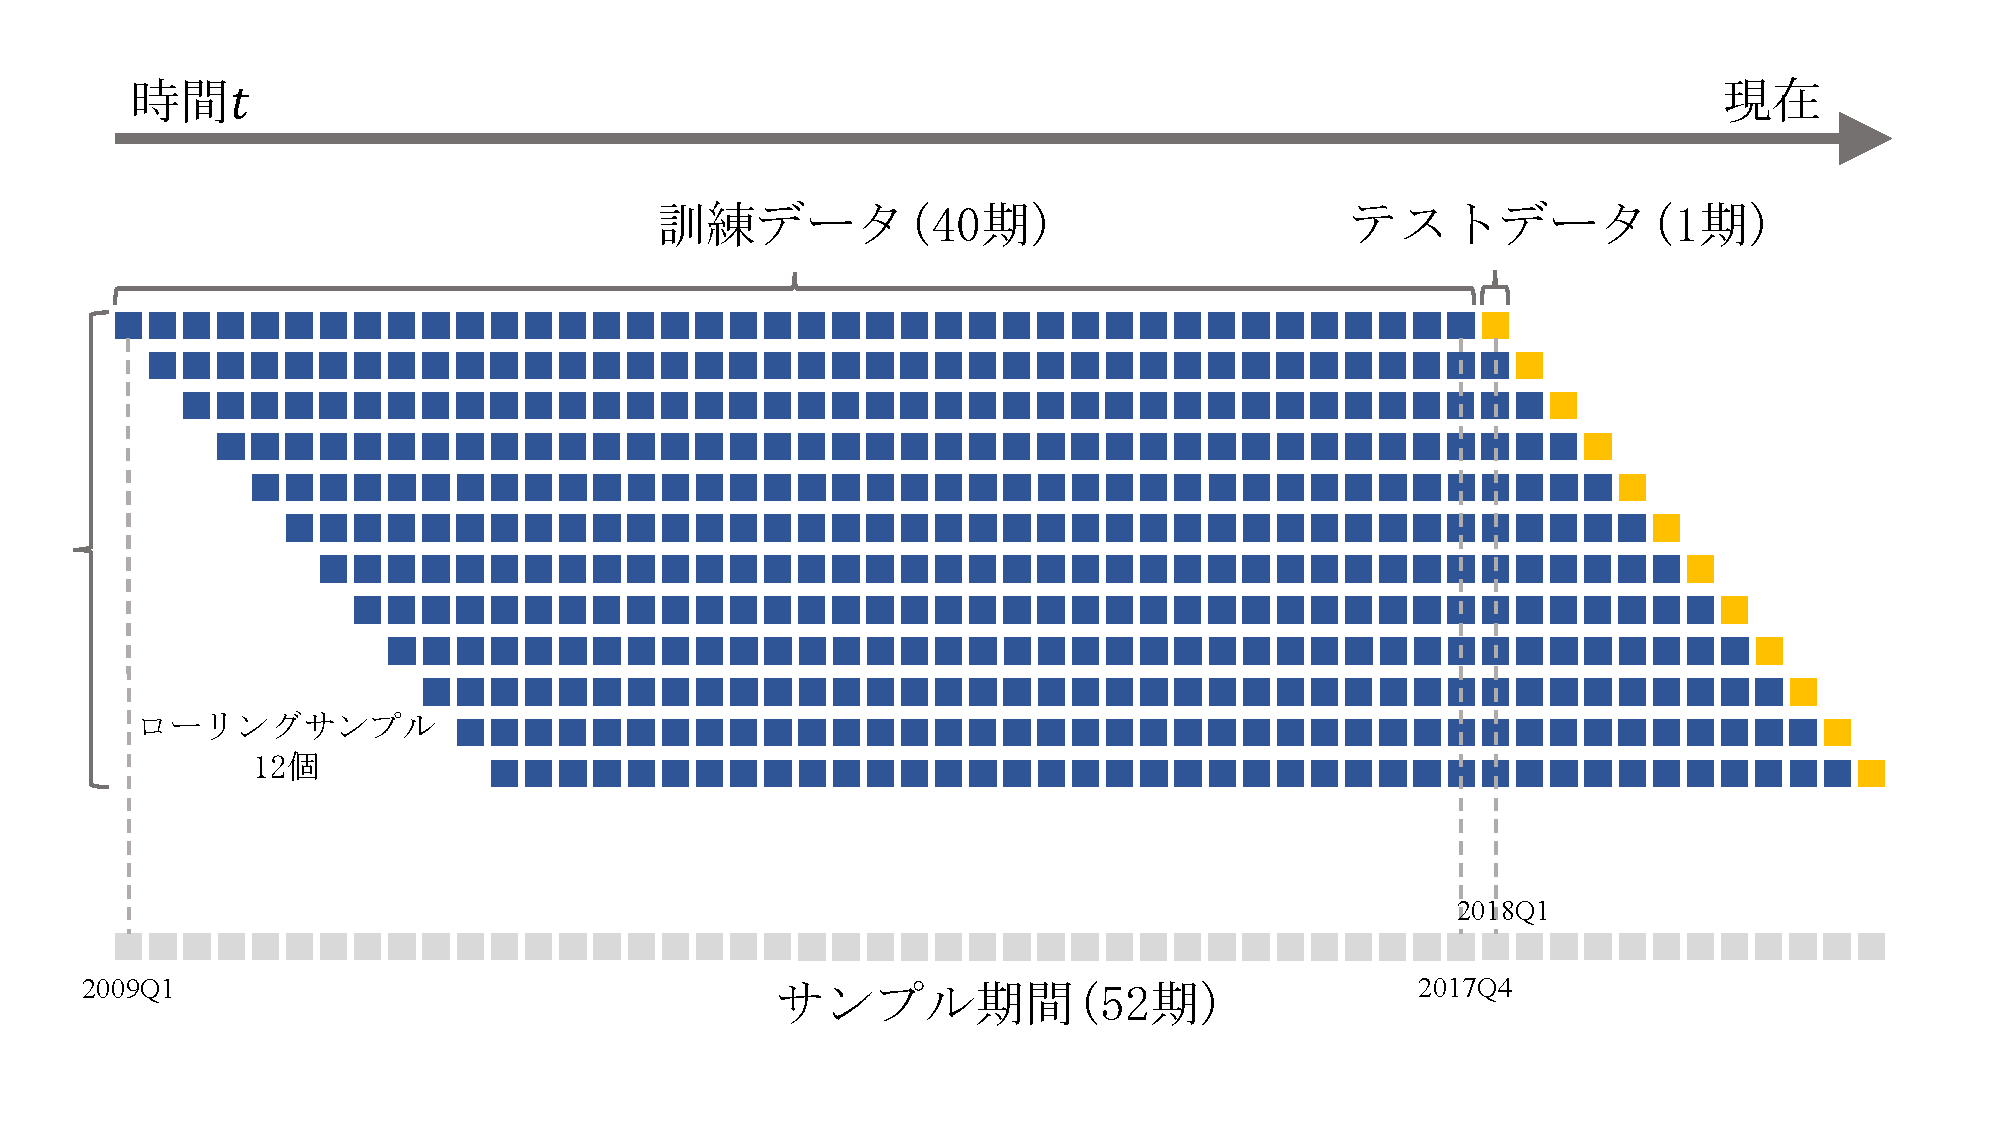
\includegraphics[width=0.8\linewidth]{./img/_rolling_sample.pdf}
  \begin{threeparttable}
  \begin{tablenotes}
    \item[](出所)筆者作成.
  \end{tablenotes}
  \end{threeparttable}  
\end{figure}

\section{伝統的時系列モデル}

\subsection{ランダムウォーク}

$Y_t$をある企業における$t$期の四半期EPSとすると,もっとも単純な単変量モデルであるランダムウォークは次のとおりである.

\begin{equation}
  \begin{split}
    & Y_t = Y_{t-1} + \epsilon_t \\
    & \hat{Y}_t^{RW} = Y_{t-1} \\
  \end{split}
\end{equation}        

%     \\
%     & ただし,\epsilon_t は全ての時点 t において \\
%     & E[\epsilon_t] = 0 \\
%     & E[\epsilon_t \epsilon_{t-k}] = \left\{
%         \begin{array}{ll}
%         \sigma^2 & k=0 \\
%         0 & k \neq 0
% \end{array}\right.\\
%     & を満たすホワイトノイズである.\\
%     \\

ただし,$\epsilon_t$は全ての時点tにおいて
\begin{equation}
  \begin{split}
    & E[\epsilon_t] = 0 \\
    & E[\epsilon_t \epsilon_{t-k}] = \left\{
      \begin{array}{ll}
        \sigma^2 & k=0 \\
        0 & k \neq 0
      \end{array}\right.\\
  \end{split}
\end{equation}    

を満たすホワイトノイズである.

一方,四半期EPS時系列には1年単位での季節的変動パターンがあると考えられる.そこでランダムウォーク過程を1四半期単位ではなく,1会計年度単位(4四半期)であると考慮した季節ランダムウォークが次のとおりである.

\begin{equation}
  \begin{split}
    & Y_t = Y_{t-4} + \epsilon_t \\
    & \hat{Y}_t^{SRW} = Y_{t-4} \\
  \end{split}
\end{equation} 

ランダムウォークは前四半期の実績値を,季節ランダムウォークは前年同四半期の実績値を予測値とするモデルであり,どちらも実際の予測においてパラメータを推定する工程がない単純なモデルである.そこで,本稿ではランダムウォーク及び季節ランダムウォークを他の予測に対するベンチマークとして用いる.

\subsection{自己回帰和分移動平均(AutoRegressive Integrated Moving Average: ARIMA)モデル}

従来の四半期EPSを予測する単変量線形時系列モデルとして,ARIMAモデル\footnote{ARIMAモデルは提唱者の名前からBox-Jenkinsモデルとも呼ばれる.},特にデータの季節性にも対応できるように一般化した季節自己回帰和分移動平均(Seasonal AutoRegressive Integrated Moving Average: SARIMA)モデルを用いる.$B^nY_t = y_{t-n}$ と定義されるような$B$(backshift operator)を導入すると,SARIMAモデルの一般形は以下のとおりである.\footnote{定数項$\theta_{\mu}=(1-\phi_1-\cdots-\phi_p)\mu$は階差をとれば0となるため,通常の取り扱いに従って0とする.}\footnote{通常,$(p,d,q) \times (P,D,Q)$の値の組み合わせはBox-Jenkins法によってデータごとに選定し,モデルの構築を行う.}

\begin{equation}
  \begin{split}
    \phi_p(B)\Phi_{P}(B)(1-B)^d(1-B^s)^DY_t &= \theta_q(B)\Theta_Q(B^s)\epsilon_t
  \end{split}
\end{equation}

ただし,
\begin{equation}
  \begin{split}
    p &: トレンドの自己回帰過程の階数 \\
    d &: トレンド階差の次数 \\
    q &: トレンドの移動平均過程の階数 \\
    P &: 季節変動の自己回帰過程の階数 \\
    D &: 季節階差の次数 \\
    Q &: 季節変動の移動平均過程の階数 \\
    s &: 季節変動の周期 \\
    \phi_p(B) &= (1 - \phi_1B - \cdots - \phi_pB^p) \\
    \theta_q(B) &= (1 - \theta_1B - \cdots - \theta_qB^q) \\
    \Phi_P(B^s) &= (1 - \Phi_1B^s - \cdots - \Phi_PB^{sP}) \\
    \Theta_Q(B^s) &= (1 - \Theta_1B^s - \cdots - \Theta_QB^{sQ}) \\
  \end{split}
\end{equation}

これまでの四半期EPSの時系列予測の分野では全ての企業に適合するSARIMAモデルが探求され,次の3つのSARIMAモデル\citep*{foster1977quarterly, griffin1977time, brown1979univariate}があらゆる企業の四半期EPSの時系列特性を描写するモデルであるとされている.
% \footnote{先行研究では,企業ごとにモデルを構築するよりも,企業で共通の構築で予測したほうが全体として予測のパフォーマンスが良いと示されている.}

\cite{foster1977quarterly} $: (p,d,q) \times (P,D,Q)_s = (1,0,0) \times (0,1,0)_4$
\begin{equation}
  \begin{split}
    % \text{ Foster (1977) } &: (p,d,q) \times (P,D,Q)_s = (1,0,0) \times (0,1,0)_4 \\
    Y_t &= Y_{t-4} + \phi_1(Y_{t-1} - Y_{t-5}) + \epsilon_t \\
    \hat{Y}_t^{ARIMA-F} &= Y_{t-4} + \phi_1(Y_{t-1} - Y_{t-5}) + \delta \\
  \end{split}
\end{equation}

\cite{griffin1977time} $: (p,d,q) \times (P,D,Q)_s = (0,1,1) \times (0,1,1)_4$
\begin{equation}
  \begin{split}
    Y_t &= Y_{t-4} + (Y_{t-1} - Y_{t-5}) - \theta_1a_{t-1} - \Theta_1a_{t-4} + \theta_1\Theta_1a_{t-5} + \epsilon_t \\
    \hat{Y}_t^{ARIMA-G} &= Y_{t-4} + (Y_{t-1} - Y_{t-5}) - \theta_1a_{t-1} - \Theta_1a_{t-4} + \theta_1\Theta_1a_{t-5} + \delta \\
  \end{split}
\end{equation}

\cite*{brown1979univariate} $: (p,d,q) \times (P,D,Q)_s = (1,0,0) \times (0,1,1)_4$
\begin{equation}
  \begin{split}    
    Y_t &= Y_{t-4} + \phi_1(Y_{t-1}-Y_{t-5}) - \Theta_1a_{t-4} + \epsilon_t \\
    \hat{Y}_t^{ARIMA-BR} &= Y_{t-4} + \phi_1(Y_{t-1}-Y_{t-5}) - \Theta_1a_{t-4} + \delta \\
    \\
  \end{split}
\end{equation}

ただし,$\delta$はSARIMAモデルの定数項である.

\noindent
本稿では先行研究に倣い,特に支持されてきたこの3つのモデルを単変量線形時系列モデルとして用いることとする.

\subsection{多変量線形回帰モデル}

ファンダメンタル会計変数が将来の四半期EPSを線形に説明するかどうかについて確かめるため,\cite*{lev1993fundamental},\cite*{abarbanell1997fundamental},\cite*{lorek1996multivariate}の研究で用いられているモデルをもとに,以下のような多変量線形回帰モデルを考える.

\begin{equation}
  \begin{split}
    \label{eq:ols1}
    \hat{Y}_t^{OLS1} = \beta_0 + \beta_1Y_{t-1} + \beta_2Y_{t-4} 
    &+ \beta_3INV_{t-1} + \beta_4AR_{t-1} + \beta_5CAPX_{t-1} \\
    &+ \beta_6GM_{t-1} + \beta_7SA_{t-1} + \beta_8ETR_{t-1} + \beta_9LF_{t-1} \\
  \end{split}
\end{equation}

\begin{equation}
  \begin{split}
    \label{eq:ols2}
    \hat{Y}_t^{OLS2} = \beta_0 + \beta_1Y_{t-1} + \beta_2Y_{t-4} 
    &+ \beta_3INV_{t-4} + \beta_4AR_{t-4} + \beta_5CAPX_{t-4} \\
    &+ \beta_6GM_{t-4} + \beta_7SA_{t-4} + \beta_8ETR_{t-4} + \beta_9LF_{t-4} \\
  \end{split}
\end{equation}

\noindent
2つのモデルはどちらも,四半期EPSの1四半期前ラグ$Y_{t-1}$と4四半期前ラグ$Y_{t-4}$が自己回帰的な説明変数として含まれている.両者の違いとしてはファンダメンタル会計変数のラグの次数にあり,式(\ref{eq:ols1})のモデルではファンダメンタル会計変数の1四半期前ラグを,式(\ref{eq:ols2})のモデルでは季節性を考慮してファンダメンタル会計変数の4四半期前ラグをモデルの説明変数として含めている.一方,\cite*{cao2009neural} は後述する機械学習アルゴリズムのモデルと利用できる情報の公平性に保つため,以下のように四半期EPSとファンダメンタル会計変数の1四半期前,2四半期前,3四半期前,4四半期前ラグをすべて含めた多変量線形回帰モデルを推定している.

\begin{equation}
  \begin{split}
    \label{eq:ols3}
    \hat{Y}_t^{OLS3} = \beta_0 + \sum^{4}_{\tau=1} \left( \beta_{1\tau}Y_{t-\tau} 
    + \beta_{2\tau}INV_{t-\tau} + \beta_{3\tau}AR_{t-\tau} + \beta_{4\tau}CAPX_{t-\tau} \right.\\
    \left.+ \beta_{5\tau}GM_{t-\tau} + \beta_{6\tau}SA_{t-\tau} + \beta_{7\tau}ETR_{t-\tau} + \beta_{8\tau}LF_{t-\tau} \right) \\
  \end{split}
\end{equation}

以上のファンダメンタル会計変数を説明変数として用いた3つの多変量線形回帰モデルを多変量モデルのベンチマークとして,機械学習アルゴリズムによる多変量予測と比較する.なお,多変量線形回帰モデルのパラメータは最小二乗法を用いてを推定する.

\section{機械学習モデル}

本節では,本稿で用いる機械学習的手法について紹介する.なお,以下より共通して時点$t$の説明変数ベクトル$\bm{X}_t$について,単変量モデルでは目的変数である四半期EPSのラグのみを用いてモデル構築を行う.

\begin{equation}
  \begin{split}
    \bm{X}_t &= (X_{t1},\ldots ,X_{tk}) \\
    &= (Y_{t-1},Y_{t-2},Y_{t-3},Y_{t-4}) \\
  \end{split}
\end{equation}

また,多変量モデルでは四半期EPSのラグに加え,ファンダメンタル会計変数のラグも含めてモデルを構築する.

\begin{equation}
  \begin{split}
    \bm{X}_t = (&X_{t1},\ldots ,X_{tk}) \\ 
    =(&Y_{t-1},Y_{t-2},Y_{t-3},Y_{t-4},\\
    & INV_{t-1},INV_{t-2},INV_{t-3},INV_{t-4},\\
    & AR_{t-1},AR_{t-2},AR_{t-3},AR_{t-4},\\
    & CAPX_{t-1},CAPX_{t-2},CAPX_{t-3},CAPX_{t-4},\\
    & GM_{t-1},GM_{t-2},GM_{t-3},GM_{t-4},\\
    & SA_{t-1},SA_{t-2},SA_{t-3},SA_{t-4},\\
    & ETR_{t-1},ETR_{t-2},ETR_{t-3},ETR_{t-4},\\ 
    & LF_{t-1},LF_{t-2},LF_{t-3},LF_{t-4}) \\
  \end{split}
\end{equation}

\subsection{罰則回帰モデル}

説明変数間に複数の強い相関が存在する場合,線形回帰モデルの最小二乗推定量の分散は大きくなる.そして高分散(high variance)により係数の推定値が極端な値をとると,訓練データ内での予測精度は高くても,テストデータにおける予測精度が低くなる恐れがある.このように予測モデルが訓練データの規則性のみを捉えてしまい,テストデータを含めたデータ全体に対して汎化できていないことを過学習(overfitting)という.

線形回帰モデルの係数の推定値が極端な値をとることに起因する過学習を防ぐために,係数の大きさに罰則を与えて推定する手法が罰則回帰モデル(penalized regression model)である\footnote{罰則回帰モデルの詳細については,\cite*{hoerl1970ridge, tibshirani1996regression, zou2005regularization}などを参照されたい.}.罰則回帰モデルは,その罰則の与え方によって推定で最小化する目的関数が異なる.本稿では罰則回帰モデルのうち,代表的なRidge回帰,LASSO回帰,Elastic Net回帰の3つを用いる.

Ridge回帰の係数は以下のように求められる.

\begin{equation} \label{eq:ridge}
  \begin{split}
    \hat{\bm{\beta}}^{Ridge} = \argmin_{\bm{\beta}}\left\{ \sum_{t=1}^{T} \left( Y_t - \beta_0 - \sum_{j=1}^{k} \beta_{j} X_{tj} \right)^2 + \lambda \sum_{j=1}^{k} \beta_{j}^{2} \right\}
  \end{split}
\end{equation}

ここで,$\lambda \geq 0$は罰則の強さを調節するパラメータであり,モデル推定の枠組みの中で決定されないパラメータ(ハイパーパラメータ)である.ハイパーパラメータの値はデータに応じて指定する必要があり,本稿におけるハイパーパラメータの選択方法の詳細については第\ref{sec:hyparam}節で説明する.式(\ref{eq:ridge})で示されるように,Ridge回帰では目的関数に係数の二乗和が含まれており,係数が過大な値をとることを防ぐ構造となっている.したがってRidge回帰は予測情報を持たない説明変数に対して係数縮小(parameter shrinkage)し,モデルの過学習を防ぐ.

LASSO(Least Absolute Shrinkage and Selection Operator)回帰の係数は以下のように求められる.

\begin{equation} \label{eq:lasso}
  \begin{split}
    \hat{\bm{\beta}}^{LASSO} = \argmin_{\bm{\beta}}\left\{ \sum_{t=1}^{T} \left( Y_t - \beta_0 - \sum_{j=1}^{k} \beta_{j} X_{tj} \right)^2 + \lambda \sum_{j=1}^{k} \left|\beta_{j}\right| \right\}
  \end{split}
\end{equation}

LASSO回帰は,Ridge回帰と同様,目的関数にパラメータのサイズに関する罰則項が含まれているが,罰則として係数の絶対値の和を用いている点がRidge回帰との違いである.この罰則の与え方により,予測情報を持たない説明変数の係数が丁度0となるスパース推定が行われる.つまり,LASSO回帰を推定することで変数選択が行われる.

Elastic Net回帰の係数は以下のように求められる.

\begin{equation}
  \begin{split}
    \hat{\bm{\beta}}^{EN} = \argmin_{\bm{\beta}}\left\{ \sum_{t=1}^{T} \left( Y_t - \beta_0 - \sum_{j=1}^{k} \beta_{j} X_{tj} \right)^2 + 
    \lambda \left\{ 
      \left( 1 - \alpha \right) \sum_{j=1}^{k} \beta_{j}^2 + 
      \alpha \sum_{j=1}^{k} \left|\beta_{j}\right| 
      \right\} 
    \right\}
  \end{split}
\end{equation}

Elastic Net回帰は,Ridge回帰とLASSO回帰の両方の罰則項を利用する構造となっている.$\alpha$はLASSO回帰の罰則の影響の割合を調節するハイパーパラメータであり,罰則の強さを調節するハイパーパラメータ$\lambda$と併せて指定する必要がある.

なお,それぞれの罰則回帰モデルの予測値は次のとおりである.

\begin{equation}
  \begin{split}
    \hat{Y}_t^{Ridge} &= \beta_0^{Ridge} + \sum_{j=1}^{k} \beta_{j}^{Ridge} X_{tj} \\
    \hat{Y}_t^{LASSO} &= \beta_0^{LASSO} + \sum_{j=1}^{k} \beta_{j}^{LASSO} X_{tj} \\
    \hat{Y}_t^{EN} &= \beta_0^{EN} + \sum_{j=1}^{k} \beta_{j}^{EN} X_{tj} \\
  \end{split}
\end{equation}

\subsection{ランダムフォレスト回帰}

ランダムフォレスト\citep{breiman2001random}は,決定木を弱学習器とするアンサンブル学習である.弱学習器とは単独で用いると精度が低い予測モデルであり,アンサンブル学習はその弱学習器を複数推定し,組み合わせることで予測精度の向上を図る手法である.弱学習器となる決定木は,ある変数のある閾値でデータを2分割し,この分割を繰り返すことで作成される.単独の決定木による予測値は,予測サンプルの説明変数をもとに作成された木の分岐を辿り,到達した末端ノードに属するサンプルの目的変数の平均値である.ランダムフォレスト回帰では,元のデータセットから標本及び変数を無作為に復元抽出した複数のサブデータセットを構築し(ブートストラップサンプリング),それをもとに弱学習器である決定木を複数推定する.そして各決定木の予測値の平均値が最終的なランダムフォレスト回帰の予測値となる.

% ランダムフォレストのイラスト?https://www.stats-guild.com/analytics/12543

決定木の数を$M$とし,$m=1,\ldots M$番目の決定木の$t$時点における予測値を$\textit{Tree}_m(\bm{X}_t)$とすると,ランダムフォレスト回帰の予測値は以下のとおりである.

\begin{equation}
  \begin{split}
    \hat{Y}_t^{RF} = \frac{1}{M} \sum_{m=1}^{M} \textit{Tree}_m(\bm{X}_t)
  \end{split}
\end{equation}

\noindent
なお,ランダムフォレスト回帰の複雑さを調節する決定木の数や決定木の分岐の回数(木の深さ)はハイパーパラメータであり,分析者が指定する必要がある.

ランダムフォレスト回帰は,ノンパラメトリックで非線形なモデルであり,説明変数と目的変数間に非線形な関係がある場合でも優れた予測が得られると考えられる.また,ブートストラップをもとに相関のない複数の決定木を推定して各決定木の予測値の平均を用いて予測を行うため,最終的な予測値の分散は小さく,予測の汎化性能が高まる性質を持つ.

\subsection{ニューラルネットワーク(Neural Network: NN)}

NNについて述べる.まずNNの構造の最小単位であるパーセプトロンについて考える.$\bm{X_t}=(X_{t1},\ldots,X_{tk})$を入力(説明変数)ベクトルとする.$(w_1,\ldots,w_k)$は入力ベクトルの要素それぞれに対応する重み(パラメータ)であり,スカラー値$b$はバイアス項(定数項)という.パーセプトロンではまず始めに$\bm{X_t}=(X_{t1},\ldots,X_{tk})$と$(w_1,\ldots,w_k)$の内積と$b$の和であるプレアクティベーション$z$を計算する.

\begin{equation}
  \begin{split}
    z = w_1 X_{t1} + \cdots + w_k X_{tk} + b
  \end{split}
\end{equation}

\noindent
次に$z$は非線形な関数である活性化関数 $\phi(\cdot)$ に渡され,アクティベーション$a$として出力される.

\begin{equation}
  \begin{split}
    a = \phi(z)
  \end{split}
\end{equation}

\noindent
以上がNNのパーセプトロンの構造であり,まとめると以下の式で表される.

\begin{equation}
  \begin{split}
    a = \phi \left(w_1 X_{t1} + \cdots + w_k X_{tk} + b \right)
  \end{split}
\end{equation}

\noindent
このパーセプトロンを複数組み合わせることで,NNが構成される.図\ref{fig:perceptron}はパーセプトロンの概要を示している.

NNと一口に言ってもその構造によって様々な種類のものがある.NNの1種である順伝播型ニューラルネットワーク(Feed-forward Neural Network: FNN)はNNのなかでも基本的な構造を持ち,全てのパーセプトロンが結合した無閉路グラフで表現されすべての計算が逐次的に行われる.FNNの最も代表的なネットワークは多層パーセプトロン(multilayer perceptron: MLP)であり,図\ref{fig:mlp}のように表される.

\begin{figure}[tbp]
  \centering
  \caption{パーセプトロンの概要}
  \label{fig:perceptron}
  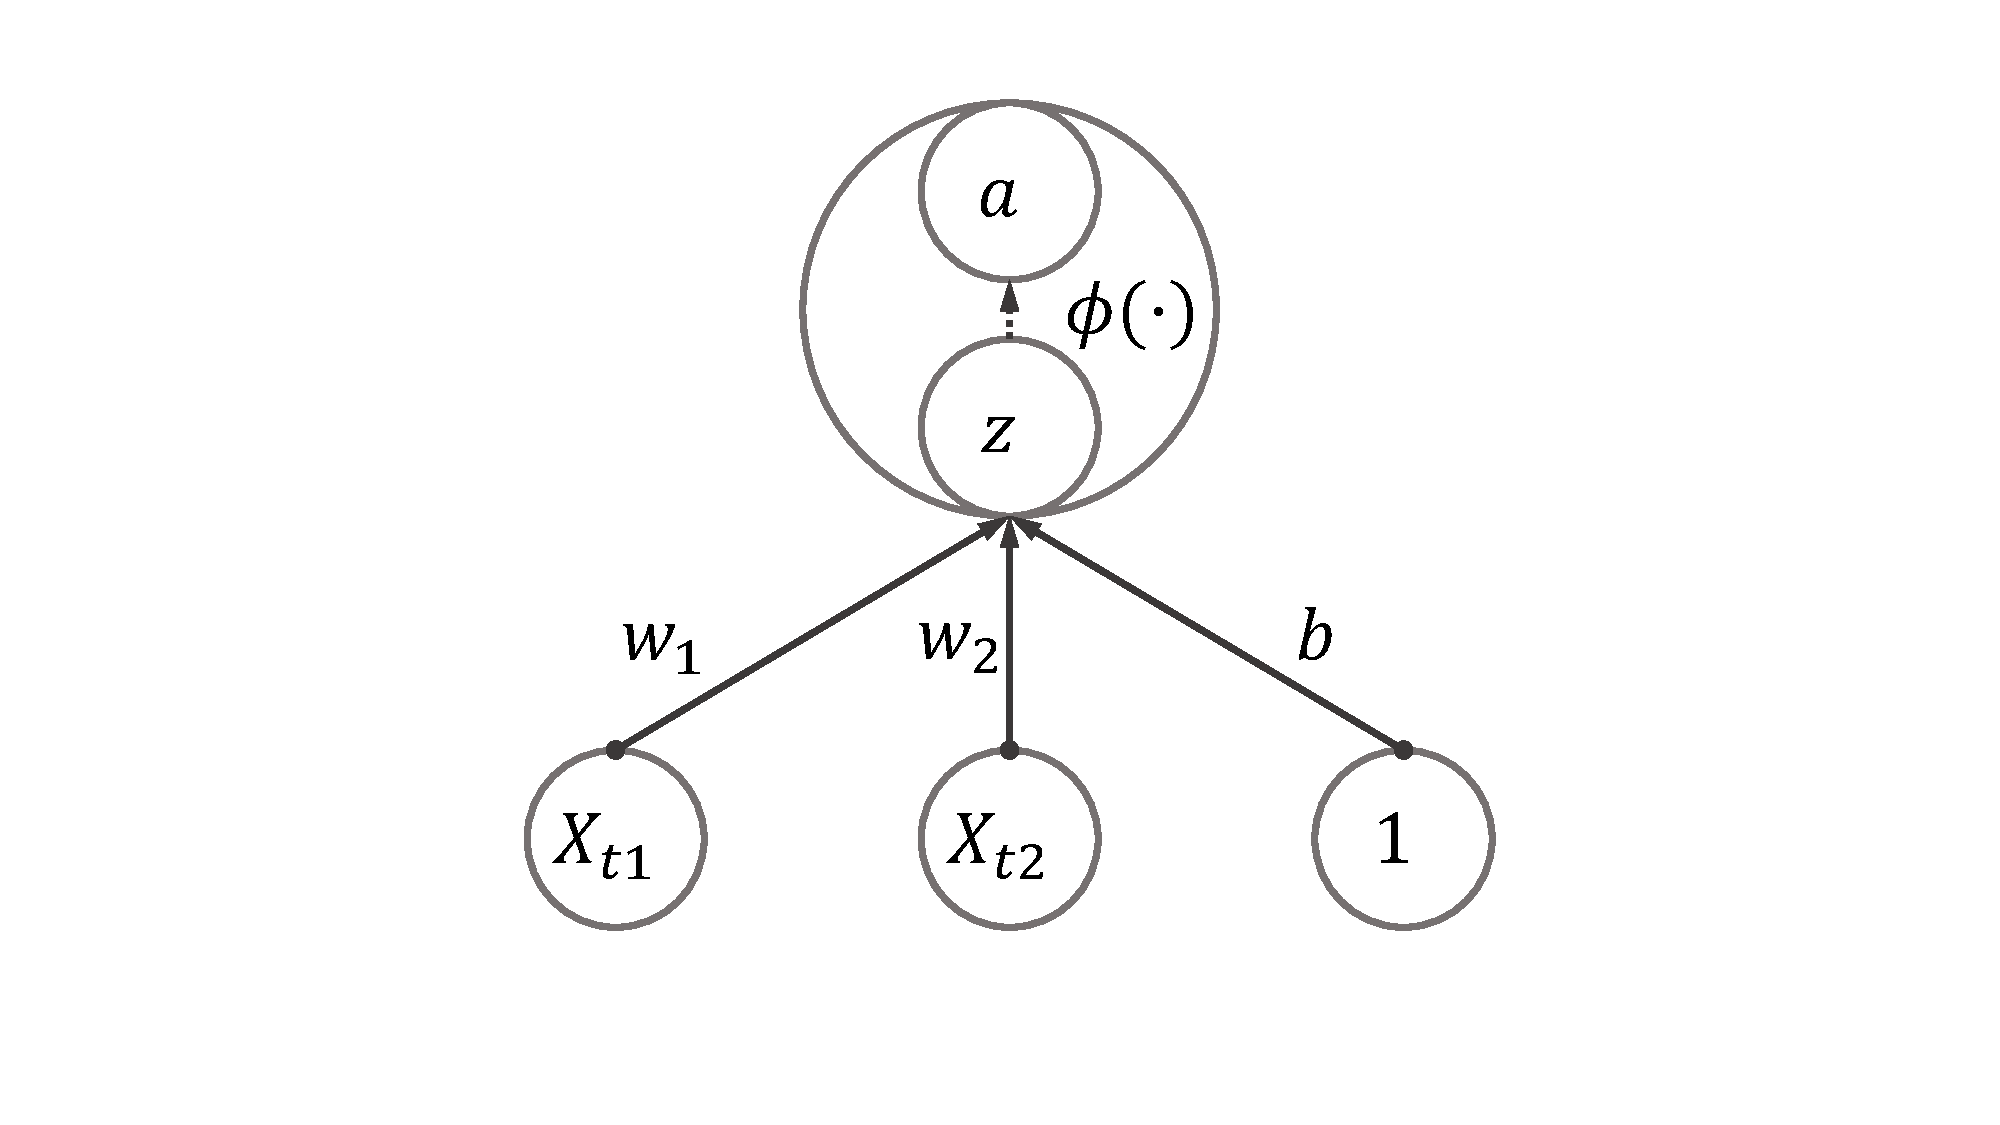
\includegraphics[width=0.4\linewidth]{./img/_ann_unit.pdf}
  \begin{threeparttable}  
  \begin{tablenotes}
    \item[](出所)筆者作成.
  \end{tablenotes}
  \end{threeparttable}  
\end{figure}

MLPの特徴として,横のつながりのパーセプトロンをそれぞれ層としてまとめると少なくとも3つ以上の層から構成される.またMLPはネットワークの全てのパーセプトロンが次の層に含まれる全てのパーセプトロンとそれぞれ結合している.ネットワークの最初の層は入力層といい入力される特徴量がここにあたる.最後の層は出力層といい,ネットワークが出力する値であり,出力層のアクティベーションは予測値を表す.この2つを除いた間の層は全て隠れ層といい,MLPの多層構造を作る.

例えば,入力層と1層の隠れ層,出力層から成る3層パーセプトロンを定式化してみる.まず,隠れ層のアクティベーションをベクトル$(H_{t1},\ldots,H_{tL})$とする.ただし,$L$は隠れ層に含まれるパーセプトロンの数である.また,隠れ層の活性関数を $\phi^{(1)}(\cdot)$ とし,隠れ層のバイアス項を$(b^{(1)}_1,\ldots,b^{(1)}_L)$とすると,隠れ層のアクティベーションは以下のように表される.

\begin{equation}
  \begin{split}
    H_{t1} &= \phi^{(1)} \left( w^{(1)}_{11} X_{t1} + w^{(1)}_{21} X_{t2} + \cdots + w^{(1)}_{k1} X_{tk} + b^{(1)}_1 \right) \\
    H_{t2} &= \phi^{(1)} \left( w^{(1)}_{12} X_{t1} + w^{(1)}_{22} X_{t2} + \cdots + w^{(1)}_{k2} X_{tk} + b^{(1)}_2 \right) \\
    \vdots \\
    H_{tL} &= \phi^{(1)} \left( w^{(1)}_{1L} X_{t1} + w^{(1)}_{2L} X_{t2} + \cdots + w^{(1)}_{kL} X_{tk} + b^{(1)}_L \right) \\
  \end{split}
\end{equation}

 次に,出力層について考える.予測する変数は本稿では1次元であるため,出力層のアクティベーションはスカラー$Y$となる.出力層の活性関数を$\phi^{(2)}(\cdot)$とし,バイアス項を$b^{(2)}$とすると,出力層のアクティベーション(または予測値)は以下のとおりである.

\begin{equation}
  \begin{split}
    \hat{Y}_t = \phi^{(2)} \left( w^{(2)}_{1} H_{t1} + w^{(2)}_{2} H_{t2} + \cdots + w^{(2)}_{L} H_{tL} + b^{(2)} \right)
  \end{split}
\end{equation}

\begin{figure}[tbp]
  \centering
  \caption{MLPの概要}
  \label{fig:mlp}
  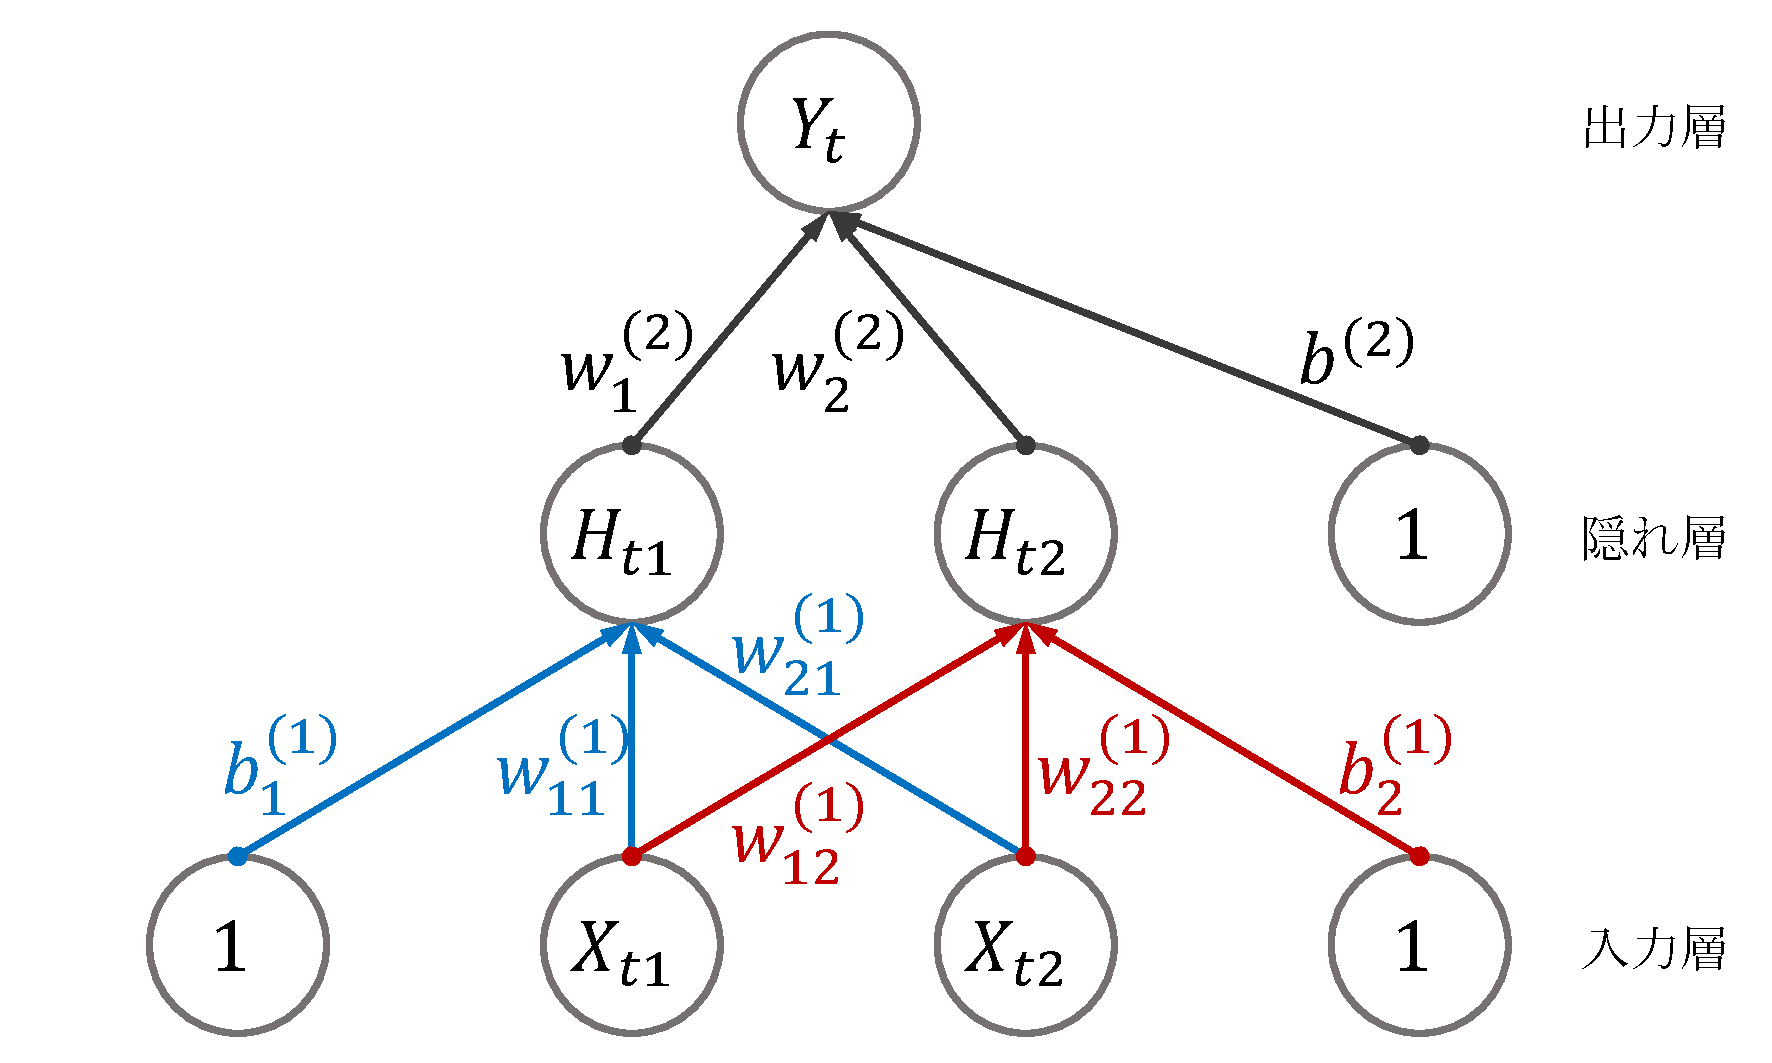
\includegraphics[width=0.6\linewidth]{./img/_ann_mlp_colored.pdf}
  \begin{threeparttable}
  \begin{tablenotes}
    \item[](出所)筆者作成.
  \end{tablenotes}
  \end{threeparttable}
\end{figure}

このように,MLPは線形結合モデルを非線形変換したものの繰り返しであることがわかる.このMLPの隠れ層の数を増やすことで,ネットワークをより深くすることができ,深層ニューラルネットワークが構築できる.一方,\cite{qi1999nonlinear}は,隠れ層のパーセプトロン数が十分であれば,隠れ層が1つで,隠れ層の活性化関数にロジスティック関数,出力層の活性化関数に恒等関数を用いた3層パーセプトロンは,あらゆる連続関数を近似できると述べている.そこで本稿は,\cite{callen1996neural}や\cite{zhang2004neural}と同様に以下のような3層パーセプトロンを用いる.

\begin{equation}
  \begin{split}
    \hat{Y}_t^{NN} 
    &= f({\bm{X}_t,\alpha,\beta}) \\
    &= \sum^{L}_{l=1} \left(\alpha_0 + \alpha_l H_{tl} \right) \\
    &= \sum^{L}_{l=1} \left\{ \alpha_0 + \alpha_l \textit{logistic} \left(\sum^{k}_{j=1} \left(\beta_{0l} + \beta_{jl} X_{tj} \right) \right) \right\} \\
  \end{split}
\end{equation}

ただし,

\begin{equation}
  \begin{split}
    \bm{X}_t &: 時点tの入力ベクトル \\
    X_{tk} &: k番目の入力 \\
    L &: 隠れ層のパーセプトロン数 \\
    \alpha_l &: 隠れ層のl番目のパーセプトロンと目的変数の重み \\
    \alpha_0 &: 出力層のバイアス項 \\
    \beta_{jl} &: j番目の入力とl番目の隠れ層のパーセプトロンの重み \\
    \beta_{0l} &: 隠れ層のl番目のパーセプトロンのバイアス項 \\
    \textit{logistic}(\cdot) = \frac{\exp(\cdot)}{1 + \exp(\cdot)} &: ロジスティック関数
  \end{split}
\end{equation}

NNの推定は誤差逆伝播法(Backward propagation algorithm)を用いて重みの勾配を計算し,勾配降下によって行う.なお,NNの複雑さを調節する隠れ層のパーセプトロン数と,重みの更新量の幅を調節する学習率はハイパーパラメータであり,分析者が指定する必要がある.

\section{ハイパーパラメータの選択} \label{sec:hyparam}

多くの機械学習アルゴリズムには,モデル推定の枠組みでは決定されない,分析者が指定する必要のあるハイパーパラメータが存在する.ハイパーパラメータの値が正しく設定できていないと,それをもとに推定されたモデルは過学習もしくは学習不足\footnote{過学習の反対語で,訓練データの規則性を十分とらえきれていないことを意味する.例えば,罰則回帰モデルの罰則の強さを表す$\lambda$の値がデータに対して大きすぎる場合,係数の大きさに対する罰則が必要以上に強く,モデルがデータの規則性を十分に学習できない可能性が生じる.}となる恐れがあり,未知のデータに対して汎化性能を持たず,高い予測精度が期待できない.そこで本稿では適切なハイパーパラメータの値を設定するため,企業ごとにグリッドサーチを行う.

具体的には,ある1企業の12個のローリングサンプルそれぞれの訓練データのうち,最新時点のデータを新たに検証データ(validation data)として分割する.例えば1つ目のローリングサンプル$\{Data_{\text{2008Q1}}, Data_{\text{2008Q2}}, \ldots, Data_{\text{2017Q3}}, Data_{\text{2017Q4}},$ $Data_{\text{2018Q1}}\}$では,訓練データを$\left\{Data_{\text{2008Q1}}, Data_{\text{2008Q2}}, \ldots, Data_{\text{2017Q3}}\right\}$,検証データを$\left\{Data_{\text{2017Q4}}\right\}$,テストデータを$\left\{Data_{\text{2018Q1}}\right\}$として3つに分割する.この分割を12個のローリングサンプルに対して行い,12個の検証データ$\left\{Data_{\text{2017Q4}}, \ldots , Data_{2020Q3}\right\}$を得る.次に,候補となるハイパーパラメータの組を用意し,全通りのハイパーパラメータをそれぞれ用いて,訓練データのみをもとに12個のモデルを推定し,検証データの目的変数を予測する.そして,検証データに対する予測能力が最も高いハイパーパラメータの組合せを最適なモデル設定であるとする.最終的には,最適なハイパーパラメータをもとに訓練データと検証データの両方を用いてモデルを再推定し,テストデータの目的変数を予測する.図\ref{fig:hyparam_selection}は本稿におけるハイパーパラメータ選択のイメージを表している.

% なお,本稿で用いた各機械学習モデルのハイパーパラメータの候補はAppendixに記載している.

\begin{figure}[tbp]
  \centering
  \caption{ハイパーパラメータ選択の概要}
  \label{fig:hyparam_selection}
  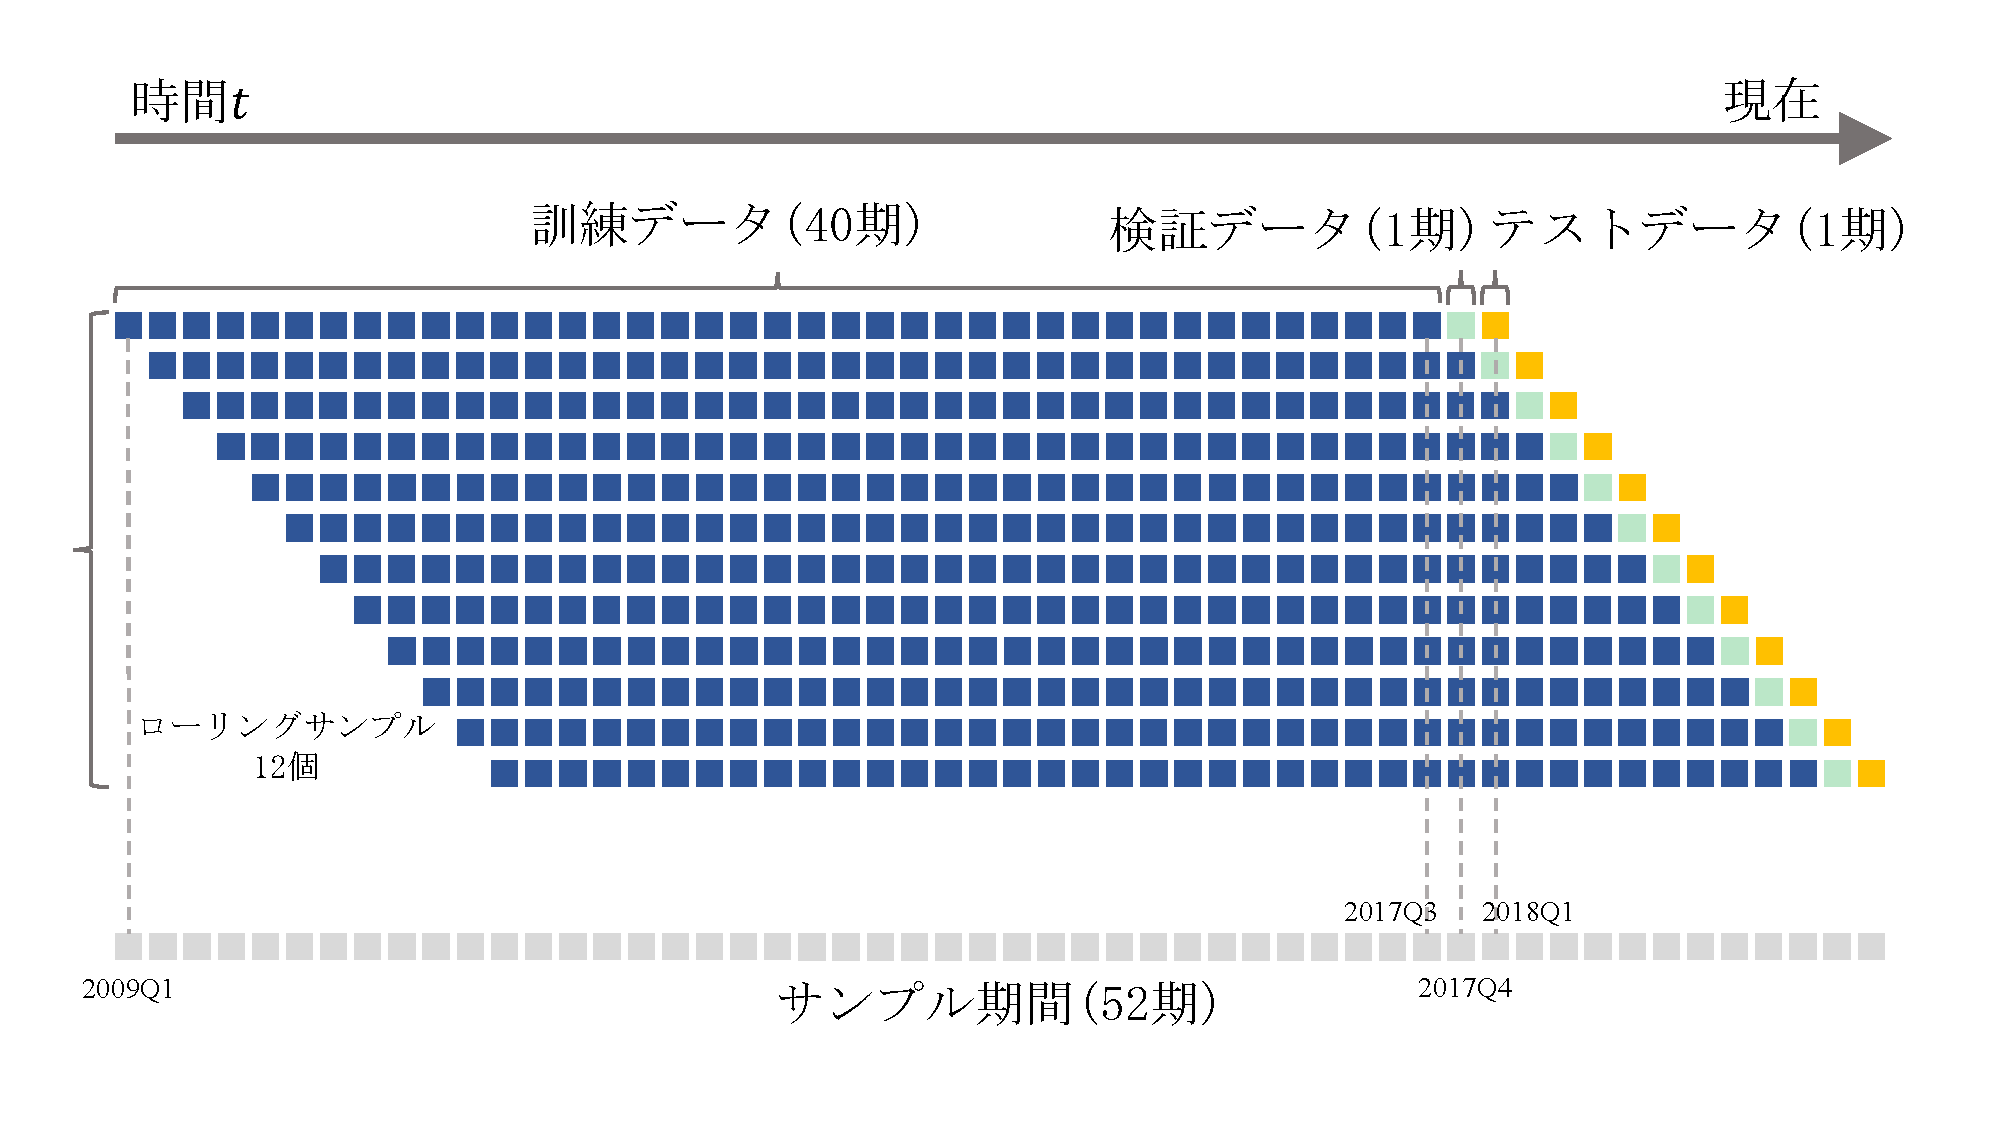
\includegraphics[width=0.8\linewidth]{./img/_rolling_sample_val.pdf}
  \begin{threeparttable}
  \begin{tablenotes}
    \item[](出所)筆者作成.
  \end{tablenotes}
  \end{threeparttable}
\end{figure}

% \part{予測精度の比較方法}

\section{予測精度指標}

各モデルの四半期EPS予測の精度を測るために,以下の予測精度指標を用いる.

平均絶対誤差(Mean Absolute Error: MAE)

\begin{equation}
  \begin{split}
    \text{MAE} = \frac {1} {T} \sum^{T}_{t=1}\left| Y_t - \hat{Y}_t \right|
  \end{split}
\end{equation}

平均絶対誤差率(Mean Absolute Percentage Error: MAPE)

\begin{equation}
  \begin{split}
    \text{MAPE} = \frac {1} {T} \sum^{T}_{t=1}\left| \frac {Y_t - \hat{Y}_t} {Y_t} \right|
  \end{split}
\end{equation}

平均二乗誤差率(Mean Squared Percentage Error: MSPE)

\begin{equation}
  \begin{split}
    \text{MSPE} = \frac {1} {T} \sum^{T}_{i=1} \left( \frac {Y_t - \hat{Y}_t} {Y_t} \right) ^2
  \end{split}
\end{equation}

\noindent
ただし,$T$は予測期間であり,本稿では2018年度第1四半期~2020年度第4四半期の12期間である.なお,MAPEとMSPEについては,\cite*{brown1979univariate},\cite*{lorek1996multivariate},\cite{zhang2004neural}に倣い絶対予測誤差率$ \left| \frac{Y_t -{\hat Y}_t}{Y_t} \right|$の上界を1とし,この制約に基づいて算出した値を報告する.また,絶対予測誤差率が1を超えるような予測サンプルをLarge Forecast Errorサンプルとし,予測精度指標の値と併せてLarge Forecast Errorの割合も報告する.

\section{Diebold-Mariano(DM)検定}

予測精度指標は異なる予測モデル間で予測精度を比較するために用いられる.ただし,精度指標の値は用いるデータセットに由来するため,精度指標の大小関係を比較するだけではモデルの精度の優劣を一般化することはできない.そこで,本稿では異なる2つの予測モデル間に統計的に有意な予測精度の差が存在するかどうかを検定するために,DM検定\citep*{diebold2002comparing}を行う.

具体的には,ある企業について,予測期間の実績値(真の値)を$\left\{Y_t ;\  t=1, \ldots, T\right\}$,異なる2つの予測モデル(モデル1とモデル2)に由来する予測値系列をそれぞれ$\left\{\hat{Y}_{1t};\  t=1, \ldots, T\right\}, \left\{\hat{Y}_{2t};\  t=1, \ldots, T\right\}$とする.このとき予測誤差系列をそれぞれ,

\begin{equation}
  \begin{split}
    \left\{ e_{1t} = \hat{Y}_{1t} - Y_t ;\  t=1, \ldots, T \right\} \\
    \left\{ e_{2t} = \hat{Y}_{2t} - Y_t ;\  t=1, \ldots, T \right\} \\
  \end{split}
\end{equation}

\noindent
とし,予測誤差の損失$L(e_t)$\footnote{損失関数$L(e_t)$は用いる予測精度指標によって異なる.例えば,MAEの場合は$L(e_t)=|e_t|$,MAPEの場合は$L(e_t)=\left|\frac{e_t}{Y_t}\right|$,MSPEの場合は$L(e_t)=\left(\frac{e_t}{Y_t}\right)^2$となる.}をもとに2つの予測誤差系列の損失差$d_{12t}$を以下のように定義する.

\begin{equation}
  \begin{split}
    d_{12t} = L(e_{1t}) - L(e_{2t})
  \end{split}
\end{equation}

\noindent
モデル1とモデル2の予測誤差に差がないとき,損失差の期待値は0となる.つまり,DM検定の帰無仮説と対立仮説は次のとおりである.

\begin{equation}
  \begin{split}
    H_0 &: E(d_{12t}) = 0,  \\
    H_1 &: E(d_{12t}) \neq 0
  \end{split}
\end{equation}

\noindent
この仮説検定を行うために以下のような検定統計量,

\begin{equation}
  \begin{split}
    DM_{12} &= \frac {\bar{d}_{12}} {s.e.(\bar{d}_{12})} \\
  \end{split}
\end{equation}

ただし,
\begin{equation}
  \begin{split}
    &\bar{d}_{12} = \frac {1} {T} \sum^{T}_{t=1} d_{12t} \\
    &s.e.(\bar{d}_{12}) は\bar{d}_{12}の標準誤差.\\
  \end{split}
\end{equation}

\noindent
を導入し,$d_{12t}$について緩い仮定の下で$DM_{12}$が標準正規分布に漸近的分布することを用いる\footnote{DM検定の詳細については\cite{diebold2002comparing}を参照されたい.}.両側DM検定で統計的に有意な検定結果が得られなければ,モデル1とモデル2の間に予測パフォーマンスの差がない結果となる.DM検定量が正の値で統計的に有意であれば,モデル1の予測誤差はモデル2よりも大きく,モデル2の方が優れた予測を与えるという結果となる.反対に,DM検定量が負の値で統計的に有意であれば,モデル1の予測誤差はモデル2よりも小さく,モデル1の方が優れた予測を与えるという結果となる.

\part{予測結果} \label{par:result}

\section{時系列モデル間の予測精度比較}

表\ref{tab:acc}は各予測指標の全企業平均を四半期別と全予測期間で集計したものを示している.まず,単変量モデル間での予測精度を比較すると,全予測期間平均でMAE,MAPE,MSPEが最も小さいモデルはランダムフォレスト回帰(それぞれ29.9,0.513,0.394),Large Forecast Errorが最小のモデルはElastic Net回帰(23.8\%)であり,いずれの指標においても機械学習アルゴリズムの予測精度が伝統的な単変量時系列モデルの予測精度を上回る結果となった.各四半期別平均についても,第1四半期や第3四半期で季節ランダムウォークに劣る場合があるものの,機械学習アルゴリズム(特にElastic Net回帰やランダムフォレスト回帰)が最も精度の高い予測を与えている.

次に,多変量モデル間での予測精度を比較してみる.全予測期間平均でMAEが最小のモデルはランダムフォレスト回帰(26.3),MAPE,MSPE,Large Forecast Errorが最小のモデルはElastic Net回帰(それぞれ0.453,0.336,20.1\%)であり,多変量モデルについても全ての指標で機械学習アルゴリズムの予測精度が伝統的な多変量線形回帰モデルの予測精度を上回る結果となった.各四半期別平均についても全ての精度指標において機械学習アルゴリズムが伝統的な多変量線形回帰モデルよりも精度の高い予測を与えている.この結果は,機械学習アルゴリズムが日本の四半期EPS予測において,1期先四半期EPSと過去の四半期EPSの実績値やファンダメンタル会計変数との関係をうまく捉えている可能性を示している.

さらに単変量モデルと多変量モデルの予測精度をを比較すると,ファンダメンタル会計変数を予測に用いることで,多変量線形回帰モデルはいずれも単変量線形時系列モデルの精度を下回る一方,多変量機械学習アルゴリズムによる予測は単変量機械学習アルゴリズムによる予測よりも精度が向上する傾向があった.この結果は\cite{zhang2004neural}と整合性があり,ファンダメンタル会計変数がもつ将来の四半期EPSを予測する情報は伝統的な線形モデルでは捉えられないことを示唆している.

推定した全ての時系列モデルの中で,多変量機械学習モデル(特にElastic Net回帰,ランダムフォレスト回帰)がいずれの精度指標や四半期別平均においても最も精度の高い予測を与えている.一方で,NNについては過去の研究から期待されるような高い精度の予測結果は得られなかった.NNの精度が低い理由として,NNは本稿で用いた他の機械学習アルゴリズムよりも推定するパラメータが桁違いに多く,よりサンプルサイズが大きいデータが必要となるため,本稿の予測のデザインではNNによる予測の精度を高めるために十分なサンプルを用意できなかったことが挙げられる.また,日本企業の四半期EPSデータは隠れ層1層で近似できない関数形である可能性も考えられ,モデルの設定やハイパーパラメータ選択が適切に行われていない可能性もある.\cite{chatfield1993neural},\cite{hill1994artificial},\cite{callen1996neural}の研究は,NNは必ずしもあらゆる時系列予測の文脈でパフォーマンスが高いモデルではないとし,NNを用いることが適切な分野とそうでない分野があると指摘している.本稿としては,日本企業の四半期EPS予測はNNにとってパフォーマンスを発揮しにくい文脈であるという結果を報告する.

なお,どの時系列モデルに関しても,第4四半期の予測が他の四半期よりも精度が低い結果となっている.過去の四半期EPS研究でも同様な傾向が確認されており,これに関して\cite{sakurai1990}は第4四半期には年次利益との一致のための利益調整が含まれているためであると解釈している.

また,一般的に異なる予測手法の予測値系列を組み合わせて\footnote{算術平均など}得る組合せ予測\citep*{bates1969combination}は個々の予測よりも精度が高い傾向があるとされる.本稿では,全時系列モデル,単変量モデル,単変量線形時系列モデル,単変量機械学習アルゴリズム,多変量モデル,多変量線形回帰モデル,多変量機械学習アルゴリズム,それぞれの組合せ予測を求めたが,いずれも目立った予測精度の向上は確認できなかった.\footnote{組み合わせ予測の予測精度は\ref{app:comb}にまとめている.}

\begin{landscape}
  \begin{table}[p]
    % \centering
    \caption{時系列モデルによる1期先四半期EPS予測の精度(1,003社平均)}
    \label{tab:acc}
    % \small
    % %%% threeparttable %%%
\begin{threeparttable}[h]

% \begin{tabular}{lrrrrrrrrrrrrrrrrrrrr}
\begin{tabular}{lrrrp{1.5cm}rrrp{1.5cm}rrrp{1.5cm}rrrp{1.5cm}rrrp{1.5cm}}
% \begin{tabularx}{6cm}{lrrrXrrrXrrrXrrrXrrrX}

\toprule
{} & \multicolumn{4}{c}{Q1} & \multicolumn{4}{c}{Q2} & \multicolumn{4}{c}{Q3} & \multicolumn{4}{c}{Q4} & \multicolumn{4}{c}{Overall} \\
\cmidrule(lr){2-5}
\cmidrule(lr){6-9}
\cmidrule(lr){10-13}
\cmidrule(lr){14-17}
\cmidrule(lr){18-21}
% \tnote
{} &    MAE \tnote{b}&   MAPE \tnote{c}&   MSPE \tnote{d}& Large Forecast Error(\%) \tnote{e}&    MAE &   MAPE &   MSPE & Large Forecast Error(\%) &    MAE &   MAPE &   MSPE & Large Forecast Error(\%) &    MAE &   MAPE &   MSPE & Large Forecast Error(\%) &     MAE &   MAPE &   MSPE & Large Forecast Error(\%) \\
% \tnote
Model \tnote{a}     &        &        &        &                         &        &        &        &                         &        &        &        &                         &        &        &        &                         &         &        &        &                         \\
\midrule
U-RW       &   44.2 &  0.668 &  0.572 &                    42.6 &   27.6 &  0.529 &  0.408 &                    25.7 &   29.7 &  0.499 &  0.372 &                    22.3 &   47.9 &  0.621 &  0.514 &                    36.1 &    37.3 &  0.579 &  0.467 &                    31.7 \\
U-SRW      &   27.1 &  0.547 &  0.436 &                    27.8 &   27.4 &  0.505 &  0.390 &                    23.8 &   26.3 &  0.461 &  0.338 &                    20.4 &   47.2 &  0.573 &  0.464 &                    32.2 &    32.0 &  0.521 &  0.407 &                    26.0 \\
U-ARIMA-F  &   32.6 &  0.549 &  0.437 &                    29.5 &   25.7 &  0.480 &  0.362 &                    22.4 &   28.3 &  0.477 &  0.355 &                    21.4 &   46.7 &  0.573 &  0.463 &                    32.3 &    33.3 &  0.520 &  0.404 &                    26.4 \\
U-ARIMA-G  &   37.7 &  0.567 &  0.460 &                    32.4 &   30.9 &  0.481 &  0.366 &                    23.9 &   33.2 &  0.488 &  0.370 &                    23.5 &   50.2 &  0.570 &  0.461 &                    31.8 &    38.0 &  0.526 &  0.414 &                    27.9 \\
U-ARIMA-BR &   36.4 &  0.559 &  0.445 &                    29.3 &   29.2 &  0.482 &  0.362 &                    22.5 &   30.1 &  0.471 &  0.348 &                    21.0 &   47.7 &  0.564 &  0.452 &                    30.1 &    35.8 &  0.519 &  0.402 &                    25.7 \\
M-OLS1     &   64.1 &  0.626 &  0.527 &                    38.8 &   50.6 &  0.556 &  0.447 &                    32.0 &   40.4 &  0.528 &  0.414 &                    27.4 &   60.9 &  0.603 &  0.499 &                    35.4 &    54.0 &  0.578 &  0.472 &                    33.4 \\
M-OLS2     &   62.5 &  0.613 &  0.514 &                    38.0 &   44.0 &  0.549 &  0.439 &                    30.8 &   77.5 &  0.569 &  0.461 &                    32.4 &   84.4 &  0.625 &  0.526 &                    38.6 &    67.1 &  0.589 &  0.485 &                    35.0 \\
M-OLS3     &  333.8 &  0.821 &  0.769 &                    67.9 &  278.6 &  0.798 &  0.738 &                    63.8 &  263.9 &  0.790 &  0.727 &                    62.0 &  225.4 &  0.797 &  0.733 &                    62.7 &   275.4 &  0.801 &  0.742 &                    64.1 \\
U-RIDGE    &   41.9 &  0.576 &  0.469 &                    33.5 &   35.4 &  0.506 &  0.391 &                    26.2 &   37.0 &  0.499 &  0.373 &                    22.2 &   49.7 &  0.575 &  0.464 &                    31.5 &    41.0 &  0.539 &  0.424 &                    28.3 \\
U-LASSO    &   35.2 &  0.591 &  0.474 &                    28.9 &   31.0 &  0.530 &  0.401 &                    21.6 &   33.9 &  0.521 &  0.385 &                    18.4 &   45.5 &  0.592 &  0.473 &                    27.9 &    36.4 &  0.559 &  0.433 &                    24.2 \\
U-EN       &   34.0 &  0.581 &  0.462 &                    28.4 &   30.7 &  0.519 &  0.390 &                    21.4 &   32.7 &  0.510 &  0.372 &                    17.7 &   45.6 &  0.591 &  0.471 &                    27.6 &    35.7 &  0.550 &  0.423 &                    23.8 \\
U-RF       &   27.1 &  0.548 &  0.435 &                    28.8 &   25.0 &  0.480 &  0.358 &                    22.2 &   26.6 &  0.464 &  0.338 &                    19.2 &   40.8 &  0.561 &  0.445 &                    29.1 &    29.9 &  0.513 &  0.394 &                    24.8 \\
U-NN       &   50.7 &  0.624 &  0.515 &                    34.4 &   49.4 &  0.580 &  0.460 &                    28.2 &   49.4 &  0.554 &  0.430 &                    25.7 &   60.5 &  0.626 &  0.516 &                    34.0 &    52.5 &  0.596 &  0.480 &                    30.6 \\
M-RIDGE    &   38.1 &  0.527 &  0.419 &                    29.3 &   33.9 &  0.483 &  0.374 &                    25.1 &   36.6 &  0.468 &  0.355 &                    24.2 &   45.7 &  0.534 &  0.429 &                    30.3 &    38.6 &  0.503 &  0.394 &                    27.2 \\
M-LASSO    &   23.6 &  0.490 &  0.374 &                    23.1 &   23.5 &  0.438 &  0.321 &                    19.1 &   24.3 &  0.422 &  0.302 &                    17.2 &   38.1 &  0.495 &  0.382 &                    24.4 &    27.4 &  0.461 &  0.345 &                    21.0 \\
M-EN       &   22.9 &  0.479 &  0.362 &                    21.8 &   22.7 &  0.425 &  0.308 &                    18.2 &   23.7 &  0.417 &  0.296 &                    16.8 &   37.7 &  0.492 &  0.377 &                    23.7 &    26.8 &  0.453 &  0.336 &                    20.1 \\
M-RF       &   24.7 &  0.495 &  0.382 &                    25.7 &   21.2 &  0.413 &  0.295 &                    17.9 &   22.7 &  0.408 &  0.287 &                    17.2 &   36.8 &  0.513 &  0.398 &                    25.8 &    26.3 &  0.457 &  0.340 &                    21.7 \\
M-NN       &   35.8 &  0.588 &  0.480 &                    33.7 &   36.8 &  0.534 &  0.416 &                    27.1 &   33.0 &  0.517 &  0.392 &                    23.4 &   46.4 &  0.595 &  0.485 &                    33.4 &    38.0 &  0.558 &  0.443 &                    29.4 \\
\bottomrule
\end{tabular}

%%% table footnote %%%
\begin{tablenotes}
\item[a] 各モデルの先頭文字列U-は単変量モデル, M-は多変量モデルを表す. また, RWはランダムウオークモデル, SRWは季節ランダムウオークモデル, ARIMA-F, ARIMA-G, ARIMA-BRはそれぞれ\cite*{foster1977quarterly, griffin1977time, brown1979univariate}の設定のARIMAモデル, OLS1, OLS2, OLS3はそれぞれ式(\ref{eq:ols1}), 式(\ref{eq:ols2}), 式(\ref{eq:ols3})の線形回帰モデル, RIDGEはRidge回帰モデル, LASSOはLASSO回帰モデル, ENはElastic Net回帰モデル, RFはランダムフォレスト回帰モデル, NNはニューラルネットワークモデルを表す.
\item[b] 平均絶対誤差(Mean Absolute Error: MAE)
\item[c] 平均絶対誤差率(Mean Absolute Percentage Error: MAPE)
\item[d] 平均二乗誤差率(Mean Squared Percentage Error: MSPE)
\item[e] 絶対予測誤差率$\left| \frac{Y_t -{\hat Y}_t}{Y_t} \right|$が1を超えるLarge Forecast Errorサンプルについては絶対予測誤差率を1としており, 表に全予測サンプルに占めるLarge Forecast Errorサンプルの割合(\%)を示している.
\end{tablenotes}
\end{threeparttable}  
    \scalebox{0.75}[0.75]{
      %%% threeparttable %%%
\begin{threeparttable}[h]

% \begin{tabular}{lrrrrrrrrrrrrrrrrrrrr}
\begin{tabular}{lrrrp{1.5cm}rrrp{1.5cm}rrrp{1.5cm}rrrp{1.5cm}rrrp{1.5cm}}
% \begin{tabularx}{6cm}{lrrrXrrrXrrrXrrrXrrrX}

\toprule
{} & \multicolumn{4}{c}{Q1} & \multicolumn{4}{c}{Q2} & \multicolumn{4}{c}{Q3} & \multicolumn{4}{c}{Q4} & \multicolumn{4}{c}{Overall} \\
\cmidrule(lr){2-5}
\cmidrule(lr){6-9}
\cmidrule(lr){10-13}
\cmidrule(lr){14-17}
\cmidrule(lr){18-21}
% \tnote
{} &    MAE \tnote{b}&   MAPE \tnote{c}&   MSPE \tnote{d}& Large Forecast Error(\%) \tnote{e}&    MAE &   MAPE &   MSPE & Large Forecast Error(\%) &    MAE &   MAPE &   MSPE & Large Forecast Error(\%) &    MAE &   MAPE &   MSPE & Large Forecast Error(\%) &     MAE &   MAPE &   MSPE & Large Forecast Error(\%) \\
% \tnote
Model \tnote{a}     &        &        &        &                         &        &        &        &                         &        &        &        &                         &        &        &        &                         &         &        &        &                         \\
\midrule
U-RW       &   44.2 &  0.668 &  0.572 &                    42.6 &   27.6 &  0.529 &  0.408 &                    25.7 &   29.7 &  0.499 &  0.372 &                    22.3 &   47.9 &  0.621 &  0.514 &                    36.1 &    37.3 &  0.579 &  0.467 &                    31.7 \\
U-SRW      &   27.1 &  0.547 &  0.436 &                    27.8 &   27.4 &  0.505 &  0.390 &                    23.8 &   26.3 &  0.461 &  0.338 &                    20.4 &   47.2 &  0.573 &  0.464 &                    32.2 &    32.0 &  0.521 &  0.407 &                    26.0 \\
U-ARIMA-F  &   32.6 &  0.549 &  0.437 &                    29.5 &   25.7 &  0.480 &  0.362 &                    22.4 &   28.3 &  0.477 &  0.355 &                    21.4 &   46.7 &  0.573 &  0.463 &                    32.3 &    33.3 &  0.520 &  0.404 &                    26.4 \\
U-ARIMA-G  &   37.7 &  0.567 &  0.460 &                    32.4 &   30.9 &  0.481 &  0.366 &                    23.9 &   33.2 &  0.488 &  0.370 &                    23.5 &   50.2 &  0.570 &  0.461 &                    31.8 &    38.0 &  0.526 &  0.414 &                    27.9 \\
U-ARIMA-BR &   36.4 &  0.559 &  0.445 &                    29.3 &   29.2 &  0.482 &  0.362 &                    22.5 &   30.1 &  0.471 &  0.348 &                    21.0 &   47.7 &  0.564 &  0.452 &                    30.1 &    35.8 &  0.519 &  0.402 &                    25.7 \\
M-OLS1     &   64.1 &  0.626 &  0.527 &                    38.8 &   50.6 &  0.556 &  0.447 &                    32.0 &   40.4 &  0.528 &  0.414 &                    27.4 &   60.9 &  0.603 &  0.499 &                    35.4 &    54.0 &  0.578 &  0.472 &                    33.4 \\
M-OLS2     &   62.5 &  0.613 &  0.514 &                    38.0 &   44.0 &  0.549 &  0.439 &                    30.8 &   77.5 &  0.569 &  0.461 &                    32.4 &   84.4 &  0.625 &  0.526 &                    38.6 &    67.1 &  0.589 &  0.485 &                    35.0 \\
M-OLS3     &  333.8 &  0.821 &  0.769 &                    67.9 &  278.6 &  0.798 &  0.738 &                    63.8 &  263.9 &  0.790 &  0.727 &                    62.0 &  225.4 &  0.797 &  0.733 &                    62.7 &   275.4 &  0.801 &  0.742 &                    64.1 \\
U-RIDGE    &   41.9 &  0.576 &  0.469 &                    33.5 &   35.4 &  0.506 &  0.391 &                    26.2 &   37.0 &  0.499 &  0.373 &                    22.2 &   49.7 &  0.575 &  0.464 &                    31.5 &    41.0 &  0.539 &  0.424 &                    28.3 \\
U-LASSO    &   35.2 &  0.591 &  0.474 &                    28.9 &   31.0 &  0.530 &  0.401 &                    21.6 &   33.9 &  0.521 &  0.385 &                    18.4 &   45.5 &  0.592 &  0.473 &                    27.9 &    36.4 &  0.559 &  0.433 &                    24.2 \\
U-EN       &   34.0 &  0.581 &  0.462 &                    28.4 &   30.7 &  0.519 &  0.390 &                    21.4 &   32.7 &  0.510 &  0.372 &                    17.7 &   45.6 &  0.591 &  0.471 &                    27.6 &    35.7 &  0.550 &  0.423 &                    23.8 \\
U-RF       &   27.1 &  0.548 &  0.435 &                    28.8 &   25.0 &  0.480 &  0.358 &                    22.2 &   26.6 &  0.464 &  0.338 &                    19.2 &   40.8 &  0.561 &  0.445 &                    29.1 &    29.9 &  0.513 &  0.394 &                    24.8 \\
U-NN       &   50.7 &  0.624 &  0.515 &                    34.4 &   49.4 &  0.580 &  0.460 &                    28.2 &   49.4 &  0.554 &  0.430 &                    25.7 &   60.5 &  0.626 &  0.516 &                    34.0 &    52.5 &  0.596 &  0.480 &                    30.6 \\
M-RIDGE    &   38.1 &  0.527 &  0.419 &                    29.3 &   33.9 &  0.483 &  0.374 &                    25.1 &   36.6 &  0.468 &  0.355 &                    24.2 &   45.7 &  0.534 &  0.429 &                    30.3 &    38.6 &  0.503 &  0.394 &                    27.2 \\
M-LASSO    &   23.6 &  0.490 &  0.374 &                    23.1 &   23.5 &  0.438 &  0.321 &                    19.1 &   24.3 &  0.422 &  0.302 &                    17.2 &   38.1 &  0.495 &  0.382 &                    24.4 &    27.4 &  0.461 &  0.345 &                    21.0 \\
M-EN       &   22.9 &  0.479 &  0.362 &                    21.8 &   22.7 &  0.425 &  0.308 &                    18.2 &   23.7 &  0.417 &  0.296 &                    16.8 &   37.7 &  0.492 &  0.377 &                    23.7 &    26.8 &  0.453 &  0.336 &                    20.1 \\
M-RF       &   24.7 &  0.495 &  0.382 &                    25.7 &   21.2 &  0.413 &  0.295 &                    17.9 &   22.7 &  0.408 &  0.287 &                    17.2 &   36.8 &  0.513 &  0.398 &                    25.8 &    26.3 &  0.457 &  0.340 &                    21.7 \\
M-NN       &   35.8 &  0.588 &  0.480 &                    33.7 &   36.8 &  0.534 &  0.416 &                    27.1 &   33.0 &  0.517 &  0.392 &                    23.4 &   46.4 &  0.595 &  0.485 &                    33.4 &    38.0 &  0.558 &  0.443 &                    29.4 \\
\bottomrule
\end{tabular}

%%% table footnote %%%
\begin{tablenotes}
\item[a] 各モデルの先頭文字列U-は単変量モデル, M-は多変量モデルを表す. また, RWはランダムウオークモデル, SRWは季節ランダムウオークモデル, ARIMA-F, ARIMA-G, ARIMA-BRはそれぞれ\cite*{foster1977quarterly, griffin1977time, brown1979univariate}の設定のARIMAモデル, OLS1, OLS2, OLS3はそれぞれ式(\ref{eq:ols1}), 式(\ref{eq:ols2}), 式(\ref{eq:ols3})の線形回帰モデル, RIDGEはRidge回帰モデル, LASSOはLASSO回帰モデル, ENはElastic Net回帰モデル, RFはランダムフォレスト回帰モデル, NNはニューラルネットワークモデルを表す.
\item[b] 平均絶対誤差(Mean Absolute Error: MAE)
\item[c] 平均絶対誤差率(Mean Absolute Percentage Error: MAPE)
\item[d] 平均二乗誤差率(Mean Squared Percentage Error: MSPE)
\item[e] 絶対予測誤差率$\left| \frac{Y_t -{\hat Y}_t}{Y_t} \right|$が1を超えるLarge Forecast Errorサンプルについては絶対予測誤差率を1としており, 表に全予測サンプルに占めるLarge Forecast Errorサンプルの割合(\%)を示している.
\end{tablenotes}
\end{threeparttable}  
    }
  \end{table}
  \end{landscape}  

\section{時系列モデル間の予測精度差の検定}

\begin{figure}[bp]
  \centering
  \caption{全企業(1,003社)のDM検定結果のまとめ(モデル1: U-SRW,loss: MAE)}
  \label{fig:dm_srw}
  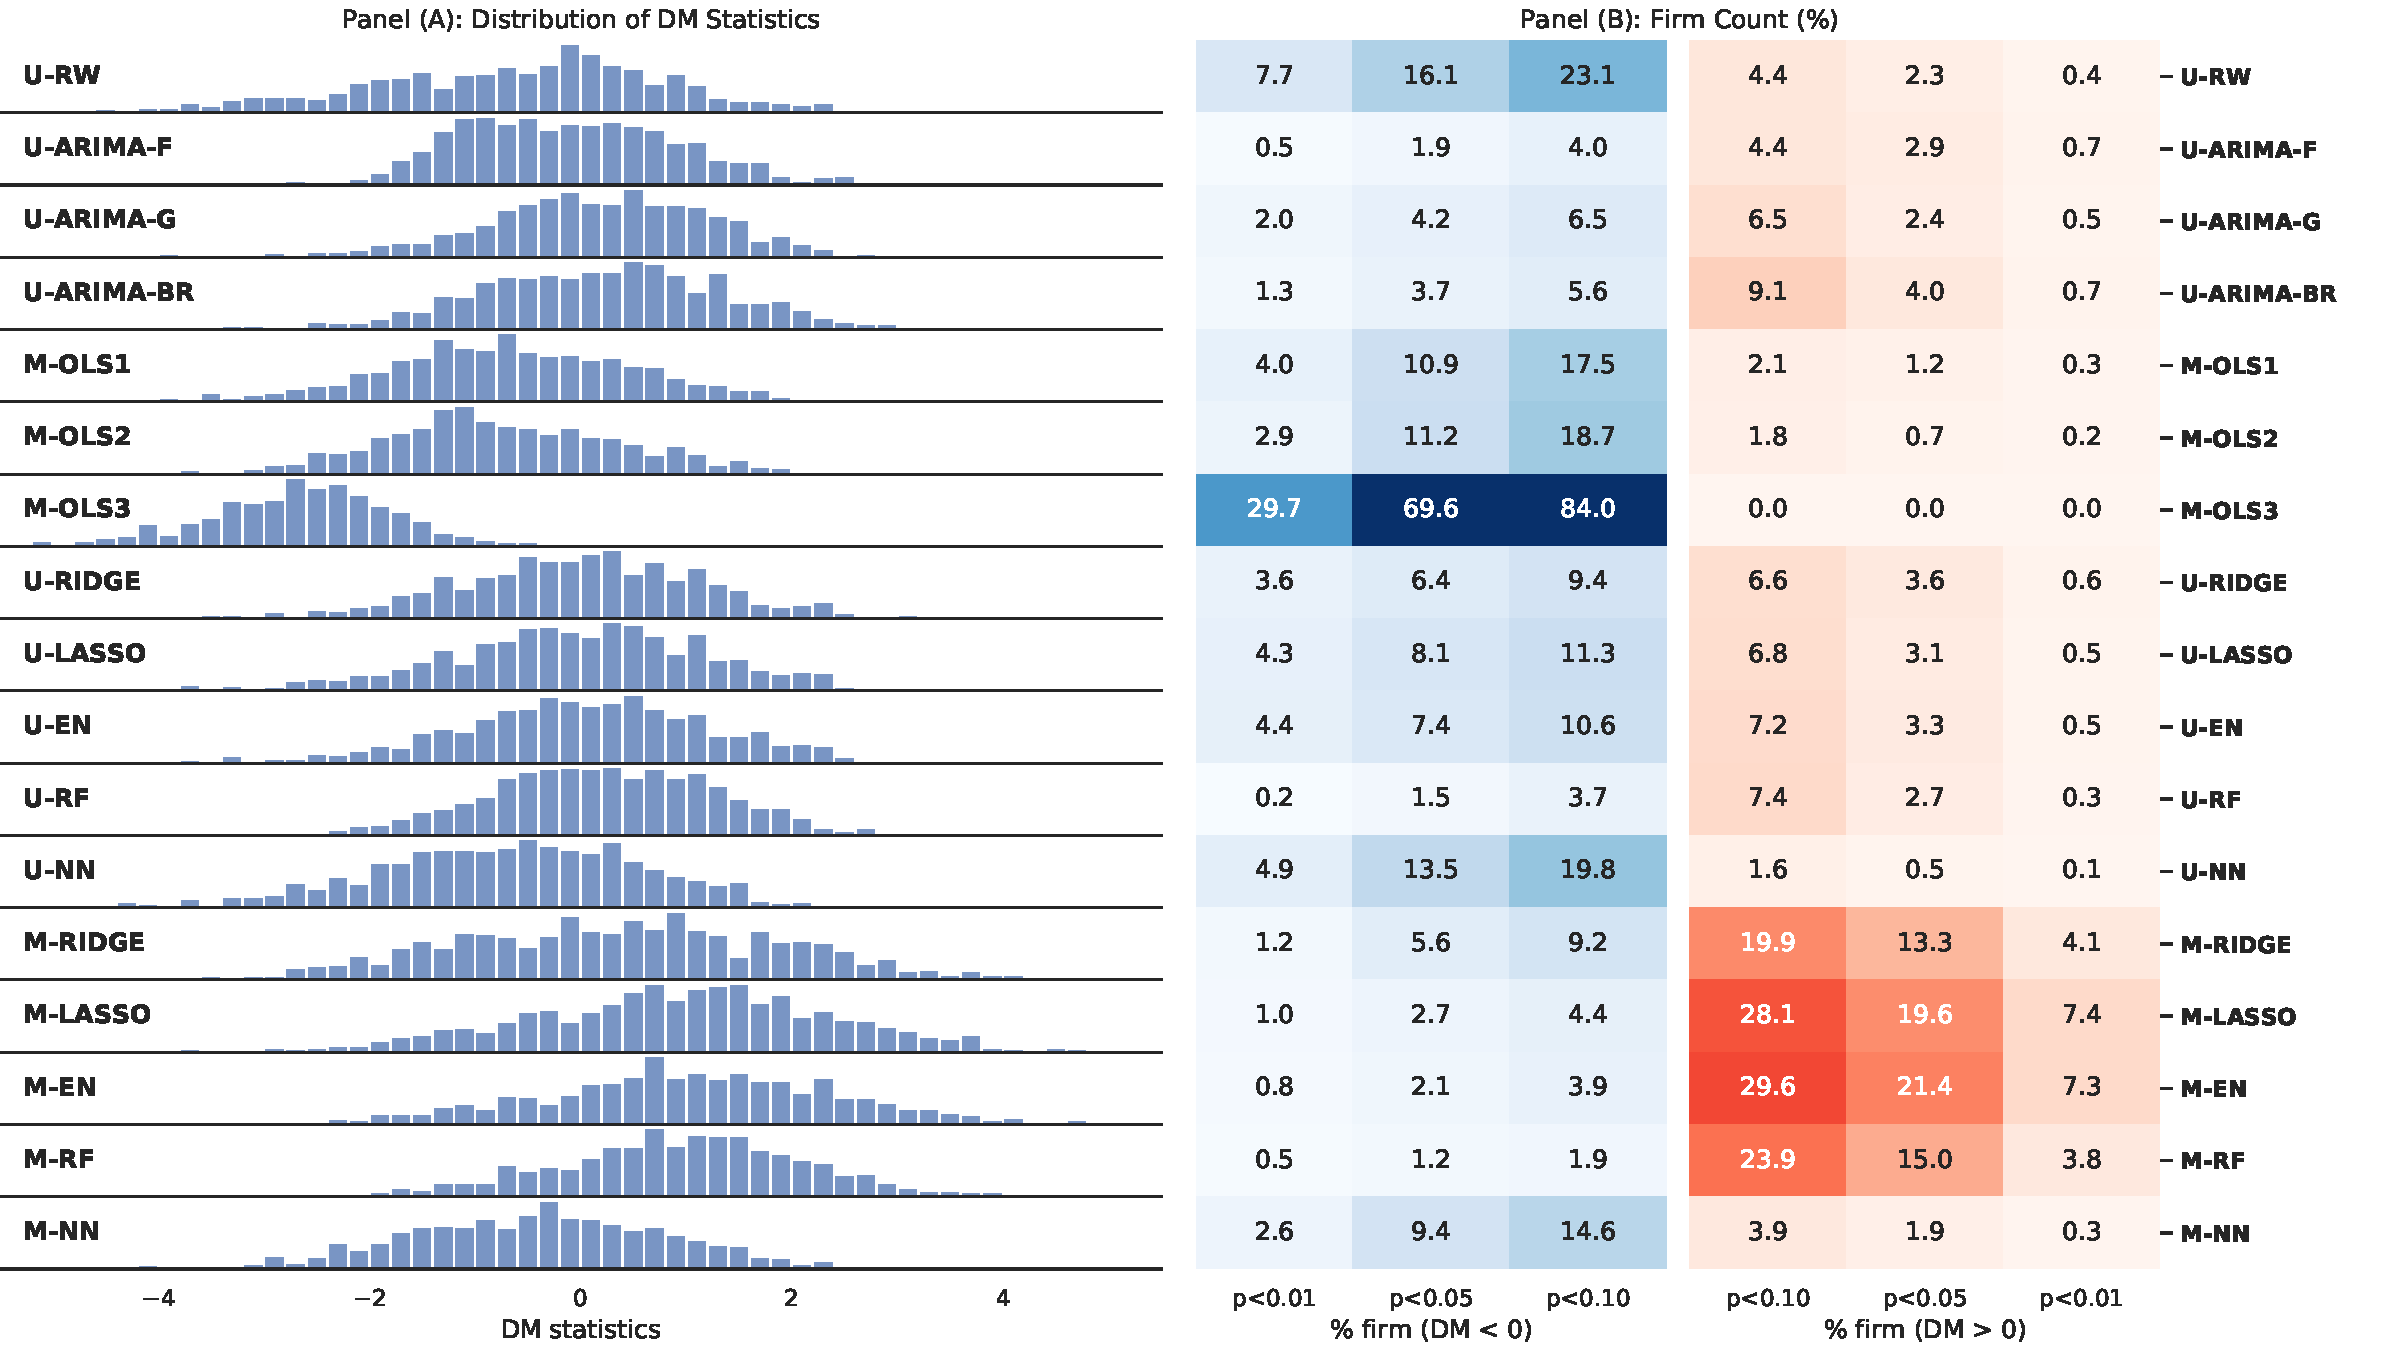
\includegraphics[width=\linewidth]{./img/_dm_MAD_y_hat_srw.pdf}
  \begin{threeparttable}
  \begin{tablenotes}
    \item[](注)各DM検定ではU-SRWをモデル1としており,損失関数はMAEに対応するもの($L(e_t)=|e_t|$)を用いている.Panel(A)はモデル2別の全1,003社のDM統計量の分布をヒストグラムで表している.Panel(B)は全1,003社のDM検定のうち,10\%,5\%,1\%の水準で統計的に有意な企業の割合(\%)をDM統計量の正負別に示したヒートマップである.色が濃いほど統計的に有意な企業の割合が大きいことを示している.
    \item[](出所)筆者作成.
  \end{tablenotes}
  \end{threeparttable}
\end{figure}

表\ref{tab:acc}において予測パフォーマンスが最も良いとされる多変量機械学習アルゴリズムが,他の時系列モデルに比べて統計的有意に予測精度が高いかどうかを検定するためにDM検定を行う.まず,ベンチマークモデルと多変量機械学習アルゴリズムの予測精度の差の統計的有意性を検定するために,季節ランダムウォークをモデル1として,その他のモデル全通りをそれぞれモデル2とした場合の両側DM検定を各企業(全1,003社)の予測値系列に対して行う.図\ref{fig:dm_srw}.Panel(A)は全1,003社のDM統計量の分布をモデル2別に示したヒストグラムであり,図\ref{fig:dm_srw}.Panel(B)は全1,003社の両側DM検定のうち,10\%,5\%,1\%の水準で統計的に有意な企業の割合(\%)をDM統計量の正負別に示したヒートマップである.なお,図\ref{fig:dm_srw}のDM検定で用いた損失関数はMAEに対応したものである\footnote{MAE以外の精度指標,MAPE,MSPEに対応する損失関数を用いたDM検定も同様な結果であった.}.

図\ref{fig:dm_srw}.Panel(A)より,モデル2が多変量Ridge回帰,LASSO回帰,Elastic Net回帰,ランダムフォレスト回帰の場合,DM統計量の分布は正の値に集中している.また,図\ref{fig:dm_srw}.Panel(B)から,先述の4つの多変量機械学習アルゴリズムにおいて,DM統計量が正の値で統計的に有意な企業の割合は,10\%水準の場合約20\%~30\%,5\%水準の場合約13\%~21\%,1\%水準の場合約4\%~7\%となっている.つまり,多変量Elastic Net回帰と多変量ランダムフォレスト回帰に加え,多変量Ridge回帰と多変量LASSO回帰も,季節ランダムウォークに比べて多くの企業で統計的有意に予測誤差が小さい結果となっており,これは多変量機械学習アルゴリズムが季節ランダムウォークよりも優れた予測を与えていることを意味する.一方,多変量線形回帰モデルについては図\ref{fig:dm_srw}.Panel(A)からDM統計量の分布は負の値に集中している,図\ref{fig:dm_srw}.Panel(B)でもDM統計量が負の値で統計的に有意な企業の割合が多いことが確認できる.つまり,線形回帰モデルはファンダメンタル会計変数を含めることでかえって予測精度が下がり,予測に何の情報も用いていない季節ランダムウォークよりも劣ってしまうことを意味する.単変量機械学習アルゴリズムについては,図\ref{fig:dm_srw}.Panel(A)と図\ref{fig:dm_srw}.Panel(B)より,統計的有意に予測精度の差がある企業が少なく,季節ランダムウォークと同程度の予測パフォーマンスであることがわかった.

\begin{figure}[tbp]
  \centering
  \caption{全企業(1,003社)のDM検定結果のまとめ(モデル1: U-ARIMA-BR,loss: MAE)}
  \label{fig:dm_sarima_br}
  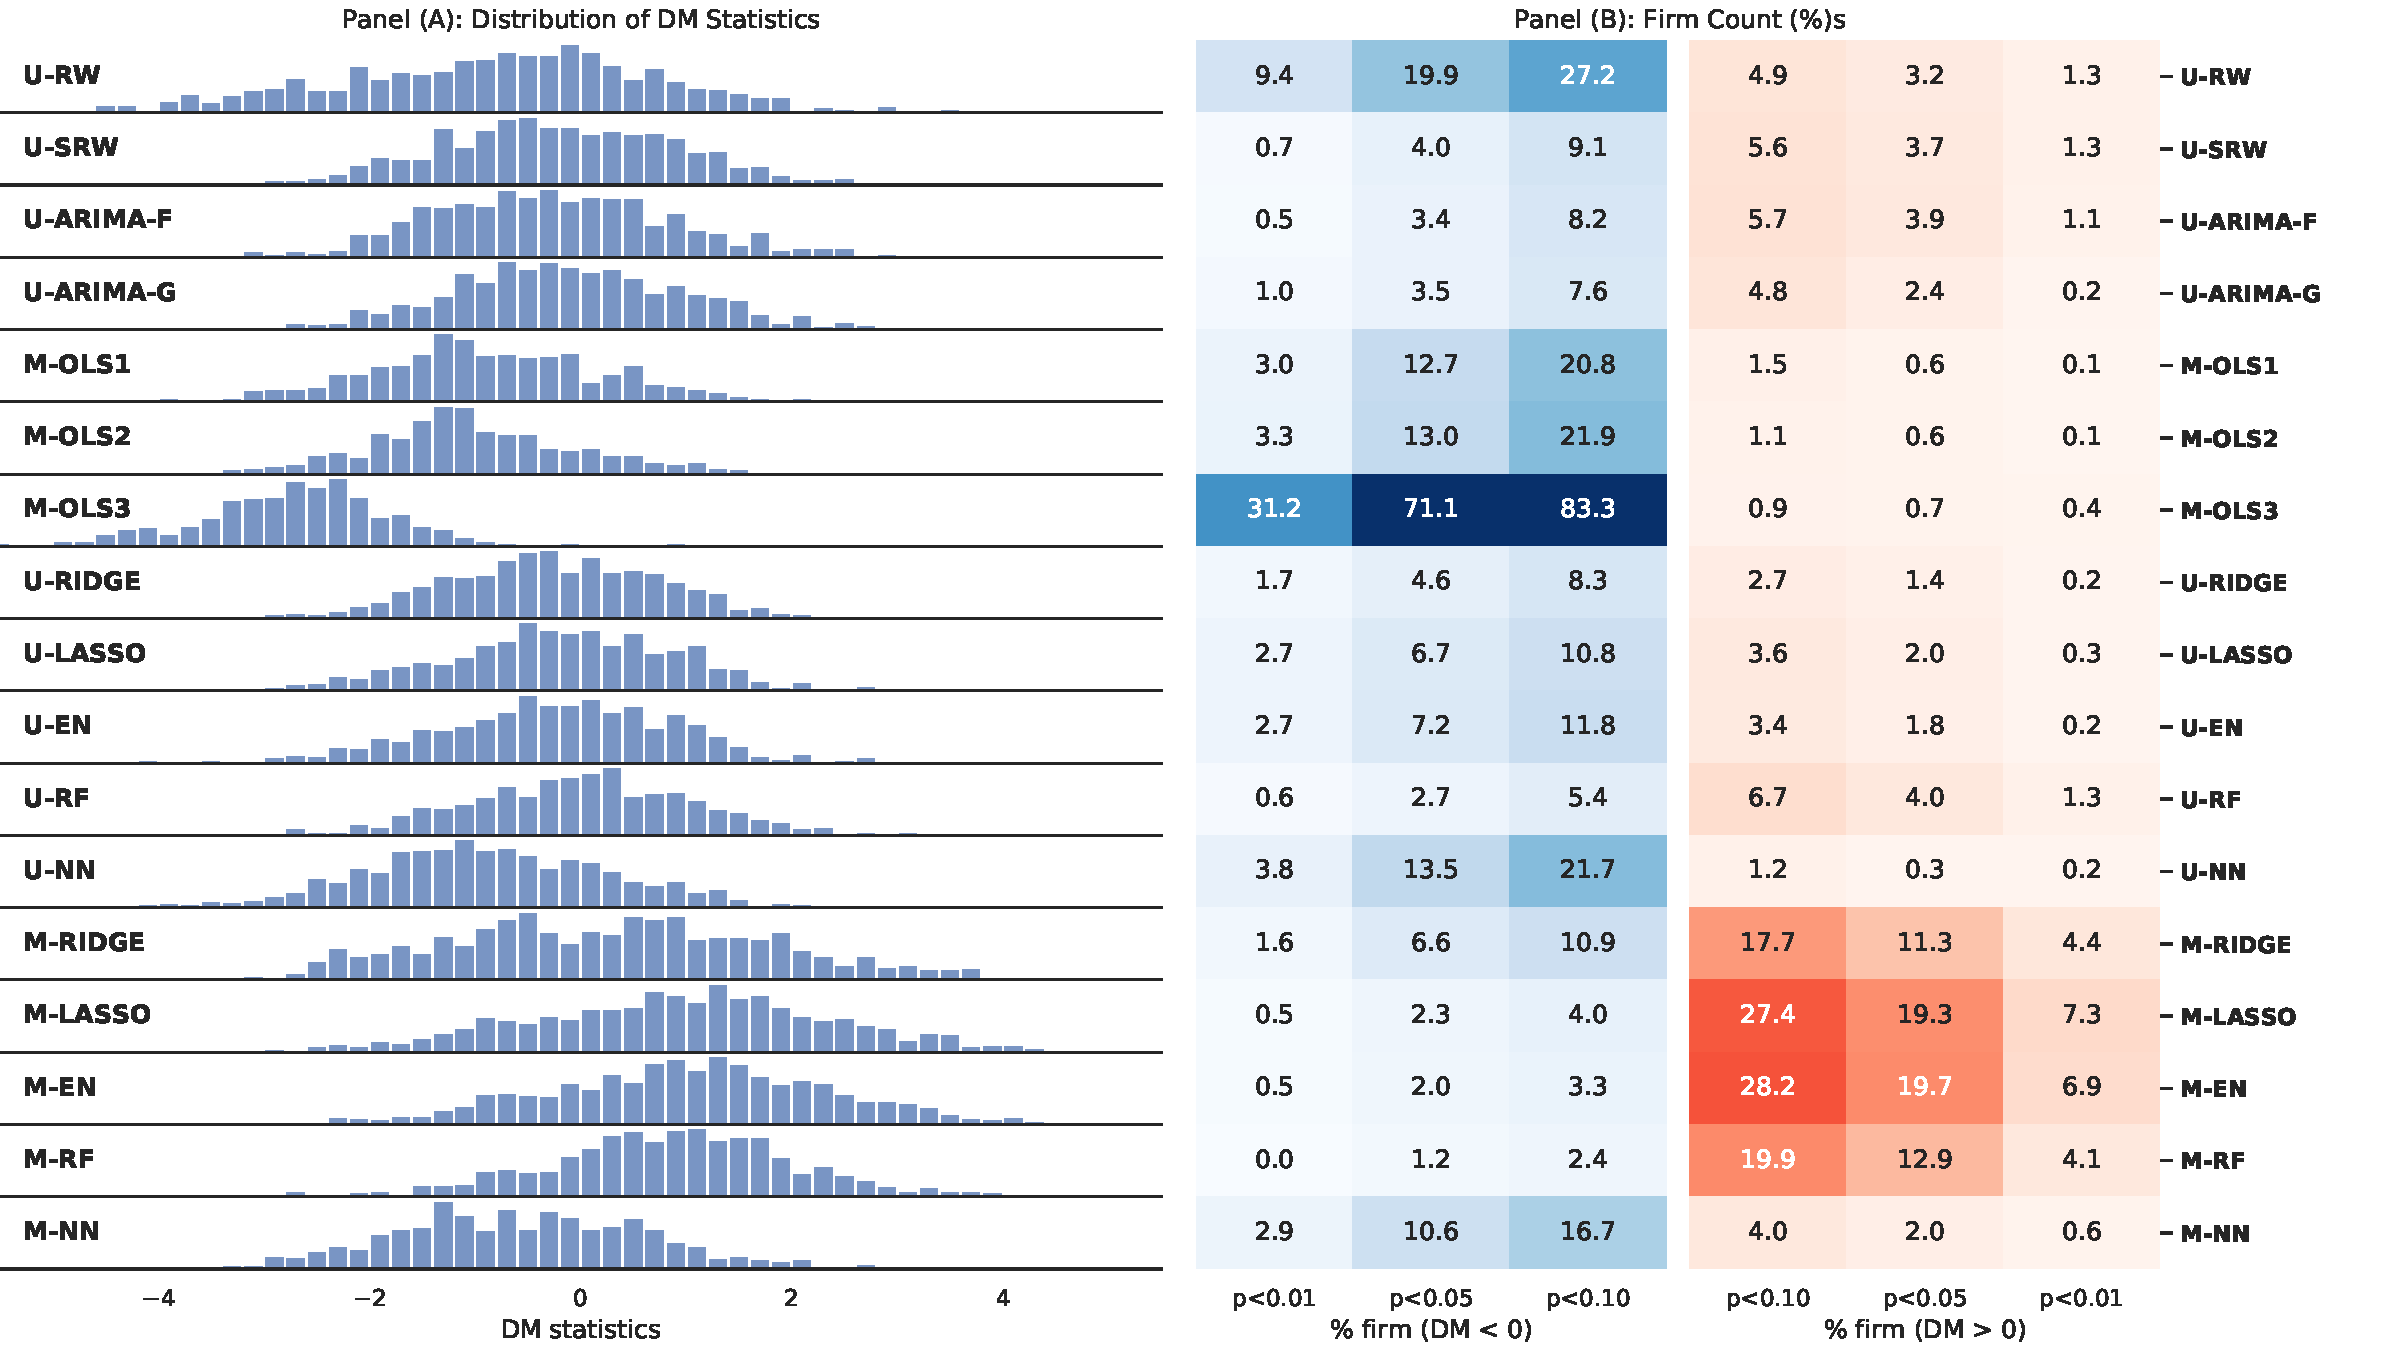
\includegraphics[width=\linewidth]{./img/_dm_MAD_y_hat_sarima_br.pdf}
  \begin{threeparttable}
  \begin{tablenotes}
    \item[](注)各DM検定ではU-ARIMA-BRをモデル1としており,損失関数はMAEに対応するもの($L(e_t)=|e_t|$)を用いている.Panel(A)はモデル2別の全1,003社のDM統計量の分布をヒストグラムで表している.Panel(B)は全1,003社のDM検定のうち,10\%,5\%,1\%の水準で統計的に有意な企業の割合(\%)をDM統計量の正負別に示したヒートマップである.色が濃いほど統計的に有意な企業の割合が大きいことを示している.
    \item[](出所)筆者作成.
  \end{tablenotes}
  \end{threeparttable}
\end{figure}

次に,伝統的線形時系列モデルと多変量機械学習アルゴリズムの予測精度の差の統計的有意性を検定するために,\cite{brown1979univariate}のARIMAモデルをモデル1として,その他のモデル全通りをそれぞれモデル2とした場合の両側DM検定を行う.図\ref{fig:dm_sarima_br}.Panel(A)は全1,003社のDM統計量の分布をモデル2別に示したヒストグラムであり,図\ref{fig:dm_sarima_br}.Panel(B)は全1,003社の両側DM検定のうち,10\%,5\%,1\%の水準で統計的に有意な企業の割合(\%)をDM統計量の正負別に示したヒートマップである.なお,図\ref{fig:dm_sarima_br}のDM検定で用いた損失関数はMAEに対応したものである\footnote{MAE以外の精度指標,MAPE,MSPEに対応する損失関数を用いたDM検定も同様な結果であった.}.

\cite{brown1979univariate}のARIMAモデルをモデル1としたDM検定の結果は,季節ランダムウォークをモデル1としたDM検定の結果と同様であった.図\ref{fig:dm_sarima_br}.Panel(A)より,モデル2が多変量Ridge回帰,LASSO回帰,Elastic Net回帰,ランダムフォレスト回帰の場合,DM統計量の分布は正の値に集中しており,図\ref{fig:dm_sarima_br}.Panel(B)からもDM統計量が正の値で統計的に有意な企業の割合が多いことが確認できる(10\%,5\%,1\%水準で統計的に有意な企業の割合は,それぞれ約18\%~28\%,11\%~20\%,4\%~7\%).つまり,多変量機械学習アルゴリズムは伝統的な線形時系列モデルである\cite{brown1979univariate}のARIMAモデルよりも多くの企業において統計的有意に予測誤差が小さく,優れた予測を与えていることを意味する\footnote{\cite{foster1977quarterly}, \cite{griffin1977time}のARIMAモデルをそれぞれモデル1としたDM検定も同様な結果であった.\ref{app:dm}参照.}

\section{アナリスト予測との予測精度比較} \label{sec:ibes}

本稿では,時系列モデルによる予測と人的な予測の精度を比較するために,人的な予測としてI/B/E/S(Institutional Brokers Estimate System)業績予想を用いる.I/B/E/S業績予想は,複数のアナリストの利益予想の平均値であるコンセンサス予想であり,日本においてもI/B/E/Sの四半期EPS予測がカバーされている企業がある\footnote{全ての上場企業はカバーされていない.}.I/B/E/S業績予想は通常,毎月第3金曜日に更新されており,本稿の時系列モデルの予測タイミングと揃えるために各四半期の中間月末(5月末,8月末,11月末,2月末)時点のI/B/E/S業績予想の1期先四半期EPS予測を比較対象とする.図\ref{fig:ibes_timing}は本稿及びI/B/E/S業績予想の四半期EPS予測のタイミングの概要を表している.

\begin{figure}[tbp]
  \centering
  \caption{I/B/E/S業績予想の更新タイミング}
  \label{fig:ibes_timing}
  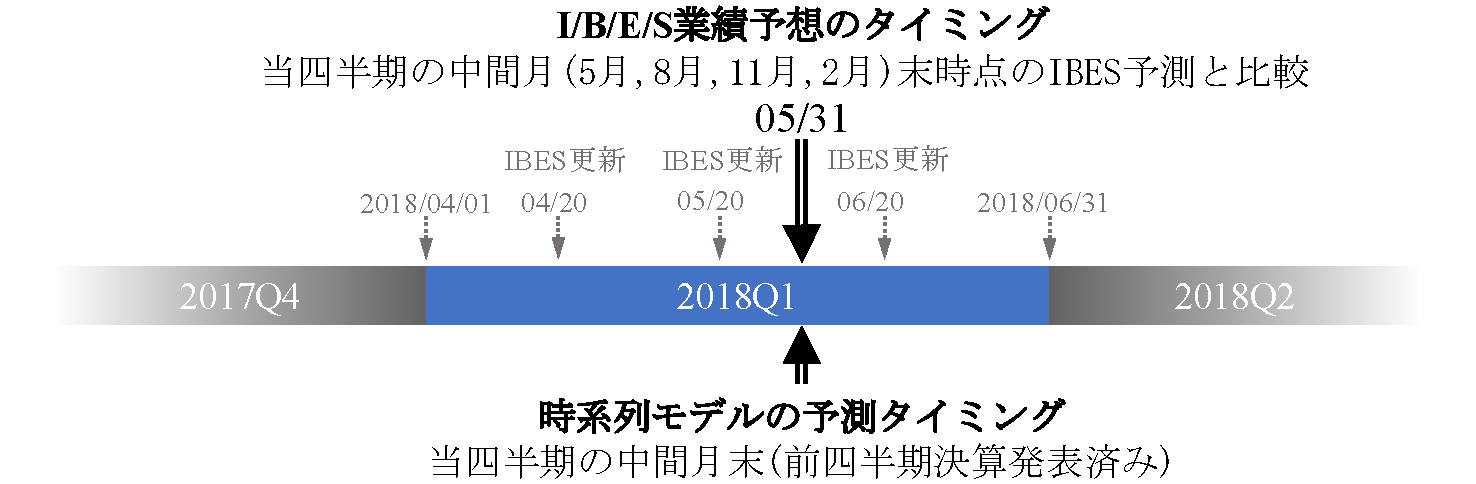
\includegraphics[width=0.60\linewidth]{./img/_ibes_timing.pdf}
  \begin{threeparttable}
  \begin{tablenotes}
    \item[](出所)筆者作成.
  \end{tablenotes}
  \end{threeparttable}
\end{figure}

本稿で用いるI/B/E/S業績予想のデータは「I/B/E/S on Datastream」から収集している.I/B/E/S業績予想のサンプル企業については,第\ref{par:data}部\ref{sec:sample}節と同様な基準のもとで選択し,予測期間についても時系列モデルと同様に2018年度第1四半期~2020年度第4四半期とする.結果として88社,延べ $88社 \times 12四半期 = 1,056個$の企業四半期予測が得られた.なお,時系列モデルとI/B/E/S業績予想の予測精度を比較するために,時系列モデルのサンプル企業については,計算可能であった1,003社からI/B/E/S業績予想が調査対象としている88社に減らして,分析対象企業をI/B/E/S業績予想と揃えることとする.表\ref{tab:acc_ibes}は時系列モデルとI/B/E/S業績予想の,各予測指標の全88社平均を四半期別と全予測期間で集計したものを示している.

全予測期間平均でMAEが最小のモデルは多変量LASSO回帰(28.7),次いで多変量Elastic Net回帰(30.1),ランダムフォレスト回帰(30.8)となり,多変量機械学習アルゴリズムがアナリスト予測であるI/B/E/S業績予想のMAE(31.5)を下回った.一方で,他の予測精度指標ではいずれもI/B/E/S業績予想が最も小さい値となり(MAPE,MSPE,Large Forecast Errorがそれぞれ0.420,0.294,16.9\%),多変量機械学習アルゴリズム(特にLASSO回帰,Elastic Net回帰,ランダムフォレスト回帰)はI/B/E/S業績予想と比較するとわずかに予測精度が低い結果となった.各四半期別平均についても同様な傾向が見られ,MAEにおいては機械学習アルゴリズムの方がI/B/E/S業績予想よりも予測精度が高いものの,他の予測精度指標ではI/B/E/S業績予想よりも予測精度が低い結果となった.

% 森(1998)は半期予測でサンプルも3社ではあるものの,伝統的時系列モデルがアナリストと遜色ない結果
% いままでの暗黙の了解とは異なる結果.
% IBESのほうがいい --> アナリストは時系列モデルで利用しファンダメンタル会計変数以外にも多くの情報を織り込んでいる.--> にもかかわらず

なお,表\ref{tab:acc}と表\ref{tab:acc_ibes}を比較すると,時系列モデルでは,もともと計算可能な1,003社平均よりもI/B/E/S業績予想が調査対象としている88社平均のほうが全体的に精度が高い傾向がみられる.そもそもアナリストは全ての上場企業をカバーしているわけではなく,限られた企業のみを調査対象としているのが日本の現状である.これについて\cite{nakai2006}は,アナリストは情報が入手しやすい企業をカバーする傾向にあると指摘しており,I/B/E/S業績予想のアナリストの調査対象企業は比較的に予測が容易である可能性が示唆される.
% 投資機会の拡張,平等な投資機会という意味でも時系列モデルはいいのでは? 米山(2010)

\begin{landscape}
  \begin{table}[p]
      % \centering
      \caption{時系列モデルによる予測とI/B/E/S業績予想の精度比較(88社平均)}
      \label{tab:acc_ibes}
      % \small
      % %%% threeparttable %%%
\begin{threeparttable}

% \begin{tabular}{lrrrrrrrrrrrrrrrrrrrr}
\begin{tabular}{lrrrp{1.5cm}rrrp{1.5cm}rrrp{1.5cm}rrrp{1.5cm}rrrp{1.5cm}}


\toprule
{} & \multicolumn{4}{c}{Q1} & \multicolumn{4}{c}{Q2} & \multicolumn{4}{c}{Q3} & \multicolumn{4}{c}{Q4} & \multicolumn{4}{c}{Overall} \\
\cmidrule(lr){2-5}
\cmidrule(lr){6-9}
\cmidrule(lr){10-13}
\cmidrule(lr){14-17}
\cmidrule(lr){18-21}
% \tnote
{} &    MAE \tnote{b}&   MAPE \tnote{c}&   MSPE \tnote{d}& Large Forecast Error(\%) \tnote{e}&    MAE &   MAPE &   MSPE & Large Forecast Error(\%) &    MAE &   MAPE &   MSPE & Large Forecast Error(\%) &    MAE &   MAPE &   MSPE & Large Forecast Error(\%) &     MAE &   MAPE &   MSPE & Large Forecast Error(\%) \\
% \tnote
Model \tnote{a}     &        &        &        &                         &        &        &        &                         &        &        &        &                         &        &        &        &                         &         &        &        &                         \\
\midrule
U-RW       &   46.0 &  0.586 &  0.465 &                    29.2 &   31.9 &  0.463 &  0.340 &                    21.6 &   39.7 &  0.443 &  0.317 &                    18.2 &   58.9 &  0.625 &  0.528 &                    37.9 &    44.1 &  0.529 &  0.413 &                    26.7 \\
U-SRW      &   35.9 &  0.491 &  0.372 &                    23.9 &   29.4 &  0.443 &  0.330 &                    22.3 &   41.8 &  0.454 &  0.331 &                    20.5 &   57.4 &  0.602 &  0.496 &                    36.0 &    41.1 &  0.498 &  0.382 &                    25.7 \\
U-ARIMA-F  &   36.6 &  0.487 &  0.374 &                    24.2 &   25.8 &  0.414 &  0.301 &                    19.7 &   41.6 &  0.457 &  0.337 &                    20.8 &   55.6 &  0.602 &  0.490 &                    33.3 &    39.9 &  0.490 &  0.376 &                    24.5 \\
U-ARIMA-G  &   37.2 &  0.522 &  0.405 &                    27.3 &   29.8 &  0.427 &  0.321 &                    21.6 &   41.4 &  0.467 &  0.344 &                    21.6 &   56.5 &  0.607 &  0.498 &                    36.4 &    41.2 &  0.506 &  0.392 &                    26.7 \\
U-ARIMA-BR &   35.8 &  0.498 &  0.380 &                    22.7 &   27.1 &  0.420 &  0.303 &                    18.2 &   36.9 &  0.434 &  0.309 &                    18.2 &   51.3 &  0.583 &  0.471 &                    31.8 &    37.8 &  0.484 &  0.365 &                    22.7 \\
\\
M-OLS1     &   49.7 &  0.574 &  0.458 &                    29.9 &   40.7 &  0.481 &  0.368 &                    26.5 &   46.5 &  0.487 &  0.368 &                    22.7 &   69.0 &  0.597 &  0.486 &                    36.0 &    51.5 &  0.535 &  0.420 &                    28.8 \\
M-OLS2     &   46.9 &  0.550 &  0.438 &                    29.2 &   39.1 &  0.480 &  0.366 &                    24.6 &   85.5 &  0.507 &  0.385 &                    25.4 &   68.1 &  0.641 &  0.548 &                    43.6 &    59.9 &  0.544 &  0.434 &                    30.7 \\
M-OLS3     &  261.9 &  0.777 &  0.712 &                    60.6 &  197.9 &  0.780 &  0.712 &                    59.8 &  207.2 &  0.747 &  0.672 &                    54.9 &  219.0 &  0.780 &  0.714 &                    60.2 &   221.5 &  0.771 &  0.703 &                    58.9 \\
\\
U-RIDGE    &   38.1 &  0.516 &  0.399 &                    26.5 &   31.7 &  0.435 &  0.311 &                    20.8 &   41.7 &  0.463 &  0.334 &                    19.3 &   49.0 &  0.592 &  0.479 &                    34.1 &    40.1 &  0.501 &  0.381 &                    25.2 \\
U-LASSO    &   35.2 &  0.529 &  0.403 &                    24.2 &   28.1 &  0.431 &  0.296 &                    16.7 &   38.5 &  0.471 &  0.335 &                    17.0 &   44.9 &  0.587 &  0.468 &                    31.8 &    36.7 &  0.504 &  0.376 &                    22.4 \\
U-EN       &   34.9 &  0.522 &  0.395 &                    23.9 &   27.7 &  0.424 &  0.292 &                    16.3 &   38.2 &  0.466 &  0.327 &                    15.9 &   44.6 &  0.584 &  0.465 &                    31.1 &    36.3 &  0.499 &  0.370 &                    21.8 \\
U-RF       &   34.2 &  0.510 &  0.389 &                    26.1 &   28.7 &  0.413 &  0.283 &                    17.4 &   38.6 &  0.460 &  0.322 &                    17.0 &   46.9 &  0.568 &  0.451 &                    30.7 &    37.1 &  0.488 &  0.361 &                    22.8 \\
U-NN       &   43.3 &  0.581 &  0.458 &                    27.3 &   35.8 &  0.507 &  0.375 &                    22.0 &   43.5 &  0.508 &  0.373 &                    20.8 &   54.0 &  0.635 &  0.525 &                    35.2 &    44.2 &  0.558 &  0.433 &                    26.3 \\
\\
M-RIDGE    &   48.2 &  0.509 &  0.402 &                    28.0 &   41.9 &  0.490 &  0.379 &                    25.4 &   44.9 &  0.461 &  0.346 &                    22.3 &   54.3 &  0.551 &  0.457 &                    34.1 &    47.3 &  0.503 &  0.396 &                    27.5 \\
M-LASSO    &   25.0 &  0.432 &  0.315 &                    18.6 &   22.4 &  0.389 &  0.263 &                    13.6 &   30.7 &  0.391 &  0.276 &                    17.4 &   36.6 &  0.488 &  0.378 &                    26.1 &    28.7 &  0.425 &  0.308 &                    18.9 \\
M-EN       &   25.8 &  0.426 &  0.310 &                    18.2 &   24.0 &  0.404 &  0.277 &                    14.8 &   31.3 &  0.407 &  0.291 &                    17.8 &   39.4 &  0.501 &  0.392 &                    27.7 &    30.1 &  0.435 &  0.318 &                    19.6 \\
M-RF       &   26.3 &  0.439 &  0.320 &                    19.7 &   22.6 &  0.375 &  0.262 &                    17.4 &   34.1 &  0.396 &  0.275 &                    18.2 &   40.2 &  0.526 &  0.410 &                    28.8 &    30.8 &  0.434 &  0.317 &                    21.0 \\
M-NN       &   41.0 &  0.536 &  0.414 &                    28.0 &   36.1 &  0.505 &  0.381 &                    25.0 &   41.3 &  0.483 &  0.355 &                    20.5 &   54.1 &  0.606 &  0.493 &                    33.0 &    43.1 &  0.532 &  0.411 &                    26.6 \\
\\
IBES       &   29.1 &  0.426 &  0.298 &                    15.9 &   26.8 &  0.390 &  0.262 &                    13.6 &   33.1 &  0.385 &  0.253 &                    12.9 &   37.1 &  0.479 &  0.364 &                    25.0 &    31.5 &  0.420 &  0.294 &                    16.9 \\
\\
\# of Forecasts     & \multicolumn{4}{c}{N=264} & \multicolumn{4}{c}{N=264} & \multicolumn{4}{c}{N=264} & \multicolumn{4}{c}{N=264} & \multicolumn{4}{c}{N=1,056} \\
\bottomrule
\end{tabular}

%%% table footnote %%%
\begin{tablenotes}
\item[a] 各モデルの先頭文字列U-は単変量モデル,M-は多変量モデルを表す. また,RWはランダムウオーク,SRWは季節ランダムウオーク,ARIMA-F,ARIMA-G,ARIMA-BRはそれぞれ\cite*{foster1977quarterly, griffin1977time, brown1979univariate}の設定のARIMAモデル,OLS1,OLS2,OLS3はそれぞれ式(\ref{eq:ols1}),式(\ref{eq:ols2}),式(\ref{eq:ols3})の線形回帰モデル,RIDGEはRidge回帰,LASSOはLASSO回帰,ENはElastic Net回帰,RFはランダムフォレスト回帰,NNはニューラルネットワークを表す.IBESはI/B/E/S業績予想を表す.
\item[b] 平均絶対誤差(Mean Absolute Error: MAE)
\item[c] 平均絶対誤差率(Mean Absolute Percentage Error: MAPE)
\item[d] 平均二乗誤差率(Mean Squared Percentage Error: MSPE)
\item[e] 絶対予測誤差率$\left| \frac{Y_t -{\hat Y}_t}{Y_t} \right|$が1を超えるLarge Forecast Errorサンプルについては絶対予測誤差率を1としており,全予測サンプルに占めるLarge Forecast Errorサンプルの割合(\%)を示している.
\item[] (出所)筆者作成. 
\end{tablenotes}
\end{threeparttable}
      \scalebox{0.75}[0.75]{
        %%% threeparttable %%%
\begin{threeparttable}

% \begin{tabular}{lrrrrrrrrrrrrrrrrrrrr}
\begin{tabular}{lrrrp{1.5cm}rrrp{1.5cm}rrrp{1.5cm}rrrp{1.5cm}rrrp{1.5cm}}


\toprule
{} & \multicolumn{4}{c}{Q1} & \multicolumn{4}{c}{Q2} & \multicolumn{4}{c}{Q3} & \multicolumn{4}{c}{Q4} & \multicolumn{4}{c}{Overall} \\
\cmidrule(lr){2-5}
\cmidrule(lr){6-9}
\cmidrule(lr){10-13}
\cmidrule(lr){14-17}
\cmidrule(lr){18-21}
% \tnote
{} &    MAE \tnote{b}&   MAPE \tnote{c}&   MSPE \tnote{d}& Large Forecast Error(\%) \tnote{e}&    MAE &   MAPE &   MSPE & Large Forecast Error(\%) &    MAE &   MAPE &   MSPE & Large Forecast Error(\%) &    MAE &   MAPE &   MSPE & Large Forecast Error(\%) &     MAE &   MAPE &   MSPE & Large Forecast Error(\%) \\
% \tnote
Model \tnote{a}     &        &        &        &                         &        &        &        &                         &        &        &        &                         &        &        &        &                         &         &        &        &                         \\
\midrule
U-RW       &   46.0 &  0.586 &  0.465 &                    29.2 &   31.9 &  0.463 &  0.340 &                    21.6 &   39.7 &  0.443 &  0.317 &                    18.2 &   58.9 &  0.625 &  0.528 &                    37.9 &    44.1 &  0.529 &  0.413 &                    26.7 \\
U-SRW      &   35.9 &  0.491 &  0.372 &                    23.9 &   29.4 &  0.443 &  0.330 &                    22.3 &   41.8 &  0.454 &  0.331 &                    20.5 &   57.4 &  0.602 &  0.496 &                    36.0 &    41.1 &  0.498 &  0.382 &                    25.7 \\
U-ARIMA-F  &   36.6 &  0.487 &  0.374 &                    24.2 &   25.8 &  0.414 &  0.301 &                    19.7 &   41.6 &  0.457 &  0.337 &                    20.8 &   55.6 &  0.602 &  0.490 &                    33.3 &    39.9 &  0.490 &  0.376 &                    24.5 \\
U-ARIMA-G  &   37.2 &  0.522 &  0.405 &                    27.3 &   29.8 &  0.427 &  0.321 &                    21.6 &   41.4 &  0.467 &  0.344 &                    21.6 &   56.5 &  0.607 &  0.498 &                    36.4 &    41.2 &  0.506 &  0.392 &                    26.7 \\
U-ARIMA-BR &   35.8 &  0.498 &  0.380 &                    22.7 &   27.1 &  0.420 &  0.303 &                    18.2 &   36.9 &  0.434 &  0.309 &                    18.2 &   51.3 &  0.583 &  0.471 &                    31.8 &    37.8 &  0.484 &  0.365 &                    22.7 \\
\\
M-OLS1     &   49.7 &  0.574 &  0.458 &                    29.9 &   40.7 &  0.481 &  0.368 &                    26.5 &   46.5 &  0.487 &  0.368 &                    22.7 &   69.0 &  0.597 &  0.486 &                    36.0 &    51.5 &  0.535 &  0.420 &                    28.8 \\
M-OLS2     &   46.9 &  0.550 &  0.438 &                    29.2 &   39.1 &  0.480 &  0.366 &                    24.6 &   85.5 &  0.507 &  0.385 &                    25.4 &   68.1 &  0.641 &  0.548 &                    43.6 &    59.9 &  0.544 &  0.434 &                    30.7 \\
M-OLS3     &  261.9 &  0.777 &  0.712 &                    60.6 &  197.9 &  0.780 &  0.712 &                    59.8 &  207.2 &  0.747 &  0.672 &                    54.9 &  219.0 &  0.780 &  0.714 &                    60.2 &   221.5 &  0.771 &  0.703 &                    58.9 \\
\\
U-RIDGE    &   38.1 &  0.516 &  0.399 &                    26.5 &   31.7 &  0.435 &  0.311 &                    20.8 &   41.7 &  0.463 &  0.334 &                    19.3 &   49.0 &  0.592 &  0.479 &                    34.1 &    40.1 &  0.501 &  0.381 &                    25.2 \\
U-LASSO    &   35.2 &  0.529 &  0.403 &                    24.2 &   28.1 &  0.431 &  0.296 &                    16.7 &   38.5 &  0.471 &  0.335 &                    17.0 &   44.9 &  0.587 &  0.468 &                    31.8 &    36.7 &  0.504 &  0.376 &                    22.4 \\
U-EN       &   34.9 &  0.522 &  0.395 &                    23.9 &   27.7 &  0.424 &  0.292 &                    16.3 &   38.2 &  0.466 &  0.327 &                    15.9 &   44.6 &  0.584 &  0.465 &                    31.1 &    36.3 &  0.499 &  0.370 &                    21.8 \\
U-RF       &   34.2 &  0.510 &  0.389 &                    26.1 &   28.7 &  0.413 &  0.283 &                    17.4 &   38.6 &  0.460 &  0.322 &                    17.0 &   46.9 &  0.568 &  0.451 &                    30.7 &    37.1 &  0.488 &  0.361 &                    22.8 \\
U-NN       &   43.3 &  0.581 &  0.458 &                    27.3 &   35.8 &  0.507 &  0.375 &                    22.0 &   43.5 &  0.508 &  0.373 &                    20.8 &   54.0 &  0.635 &  0.525 &                    35.2 &    44.2 &  0.558 &  0.433 &                    26.3 \\
\\
M-RIDGE    &   48.2 &  0.509 &  0.402 &                    28.0 &   41.9 &  0.490 &  0.379 &                    25.4 &   44.9 &  0.461 &  0.346 &                    22.3 &   54.3 &  0.551 &  0.457 &                    34.1 &    47.3 &  0.503 &  0.396 &                    27.5 \\
M-LASSO    &   25.0 &  0.432 &  0.315 &                    18.6 &   22.4 &  0.389 &  0.263 &                    13.6 &   30.7 &  0.391 &  0.276 &                    17.4 &   36.6 &  0.488 &  0.378 &                    26.1 &    28.7 &  0.425 &  0.308 &                    18.9 \\
M-EN       &   25.8 &  0.426 &  0.310 &                    18.2 &   24.0 &  0.404 &  0.277 &                    14.8 &   31.3 &  0.407 &  0.291 &                    17.8 &   39.4 &  0.501 &  0.392 &                    27.7 &    30.1 &  0.435 &  0.318 &                    19.6 \\
M-RF       &   26.3 &  0.439 &  0.320 &                    19.7 &   22.6 &  0.375 &  0.262 &                    17.4 &   34.1 &  0.396 &  0.275 &                    18.2 &   40.2 &  0.526 &  0.410 &                    28.8 &    30.8 &  0.434 &  0.317 &                    21.0 \\
M-NN       &   41.0 &  0.536 &  0.414 &                    28.0 &   36.1 &  0.505 &  0.381 &                    25.0 &   41.3 &  0.483 &  0.355 &                    20.5 &   54.1 &  0.606 &  0.493 &                    33.0 &    43.1 &  0.532 &  0.411 &                    26.6 \\
\\
IBES       &   29.1 &  0.426 &  0.298 &                    15.9 &   26.8 &  0.390 &  0.262 &                    13.6 &   33.1 &  0.385 &  0.253 &                    12.9 &   37.1 &  0.479 &  0.364 &                    25.0 &    31.5 &  0.420 &  0.294 &                    16.9 \\
\\
\# of Forecasts     & \multicolumn{4}{c}{N=264} & \multicolumn{4}{c}{N=264} & \multicolumn{4}{c}{N=264} & \multicolumn{4}{c}{N=264} & \multicolumn{4}{c}{N=1,056} \\
\bottomrule
\end{tabular}

%%% table footnote %%%
\begin{tablenotes}
\item[a] 各モデルの先頭文字列U-は単変量モデル,M-は多変量モデルを表す. また,RWはランダムウオーク,SRWは季節ランダムウオーク,ARIMA-F,ARIMA-G,ARIMA-BRはそれぞれ\cite*{foster1977quarterly, griffin1977time, brown1979univariate}の設定のARIMAモデル,OLS1,OLS2,OLS3はそれぞれ式(\ref{eq:ols1}),式(\ref{eq:ols2}),式(\ref{eq:ols3})の線形回帰モデル,RIDGEはRidge回帰,LASSOはLASSO回帰,ENはElastic Net回帰,RFはランダムフォレスト回帰,NNはニューラルネットワークを表す.IBESはI/B/E/S業績予想を表す.
\item[b] 平均絶対誤差(Mean Absolute Error: MAE)
\item[c] 平均絶対誤差率(Mean Absolute Percentage Error: MAPE)
\item[d] 平均二乗誤差率(Mean Squared Percentage Error: MSPE)
\item[e] 絶対予測誤差率$\left| \frac{Y_t -{\hat Y}_t}{Y_t} \right|$が1を超えるLarge Forecast Errorサンプルについては絶対予測誤差率を1としており,全予測サンプルに占めるLarge Forecast Errorサンプルの割合(\%)を示している.
\item[] (出所)筆者作成. 
\end{tablenotes}
\end{threeparttable}
      }
  \end{table}
  \end{landscape}

\section{アナリスト予測との予測精度差の検定}

\begin{figure}[bp]
  \centering
  \caption{全企業(88社)のDM検定結果のまとめ(モデル1: IBES,loss: MAE)}
  \label{fig:dm_ibes_mad}
  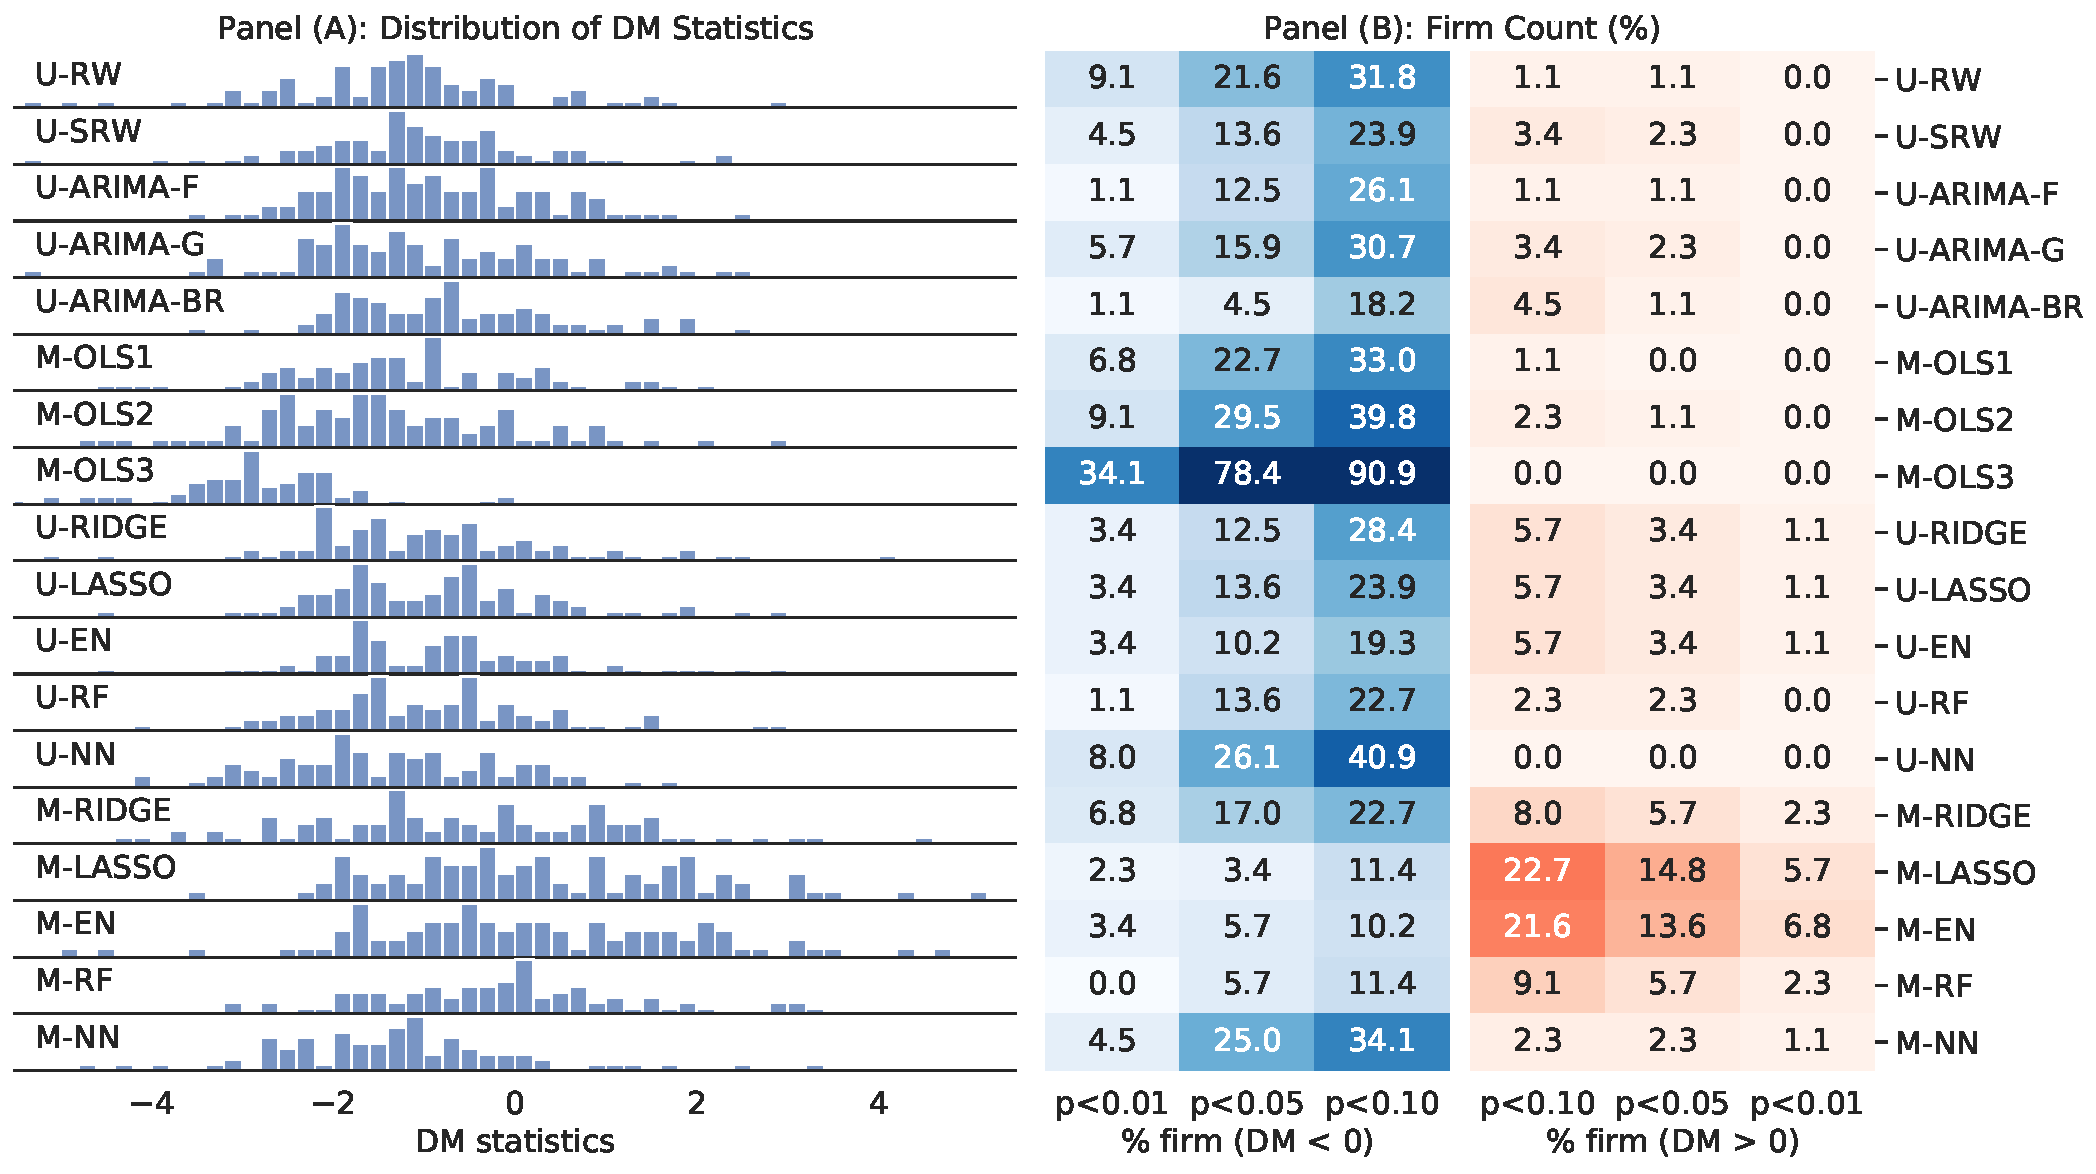
\includegraphics[width=\linewidth]{./img/_dm_MAD_y_hat_ibes.pdf}
  \begin{threeparttable}
  \begin{tablenotes}
    \item[](注)各DM検定ではIBESをモデル1としており,損失関数はMAEに対応するもの($L(e_t)=|e_t|$)を用いている.Panel(A)はモデル2別の全88社のDM統計量の分布をヒストグラムで表している.Panel(B)は全88社のDM検定のうち,10\%,5\%,1\%の水準で統計的に有意な企業の割合(\%)をDM統計量の正負別に示したヒートマップである.色が濃いほど統計的に有意な企業の割合が大きいことを示している.
    \item[](出所)筆者作成.
  \end{tablenotes}
  \end{threeparttable}
\end{figure}

まず,表\ref{tab:acc_ibes}でMAEがI/B/E/S業績予想よりも小さい多変量LASSO回帰,Elastic Net回帰,ランダムフォレスト回帰が,I/B/E/S業績予想と比べて統計的有意に予測誤差が小さいかどうかをDM検定する.具体的にはI/B/E/S業績予想をモデル1として,その他のモデル全通りをそれぞれモデル2とした場合の,損失関数をMAEに対応するものとした両側DM検定を,I/B/E/S業績予想が調査の対象としている企業(全88社)の予測値系列に対して行う.図\ref{fig:dm_ibes_mad}.Panel(A)は全88社のDM統計量の分布をモデル2別に示したヒストグラムであり,図\ref{fig:dm_ibes_mad}.Panel(B)は全88社の両側DM検定のうち,10\%,5\%,1\%の水準で統計的に有意な企業の割合(\%)をDM統計量の正負別に示したヒートマップである.

図\ref{fig:dm_ibes_mad}.Panel(A)より,多くの時系列モデルでDM統計量の分布が負の値に集中している.図\ref{fig:dm_ibes_mad}.Panel(B)でも多くの時系列モデルにおいてDM統計量が負の値で統計的に有意な企業の割合が多いことが確認でき,アナリスト予測は単変量線形時系列モデル,多変量線形回帰モデル,単変量機械学習アルゴリズムによる予測よりも精度が高いことを示している.一方,I/B/E/S業績予想と多変量機械学習アルゴリズムの検定結果では,図\ref{fig:dm_ibes_mad}.Panel(A)より,モデル2が多変量LASSO回帰とElastic Net回帰のときDM検定量の分布が正の値に集中しており,図\ref{fig:dm_ibes_mad}.Panel(B)から,DM統計量が正の値で統計的に有意な企業の割合が多いことが確認できる(10\%,5\%,1\%水準で統計的に有意な企業の割合は,それぞれ約22~23\%,14~15\%,6~7\%).つまり,MAEにおいて多変量機械学習アルゴリズムはアナリスト予測であるI/B/E/S業績予想よりも多くの企業において統計的有意に予測誤差が小さく,優れた予測を与えていることを意味する.なお,モデル2が多変量ランダムフォレスト回帰の場合は有意水準と統計的有意に異なった企業の割合が同程度であり,I/B/E/S業績予想と多変量ランダムフォレスト回帰の予測精度に差はない結果となった.

\begin{figure}[tbp]
  \centering
  \caption{全企業(88社)のDM検定結果のまとめ(モデル1: IBES,loss: MAPE)}
  \label{fig:dm_ibes_mape}
  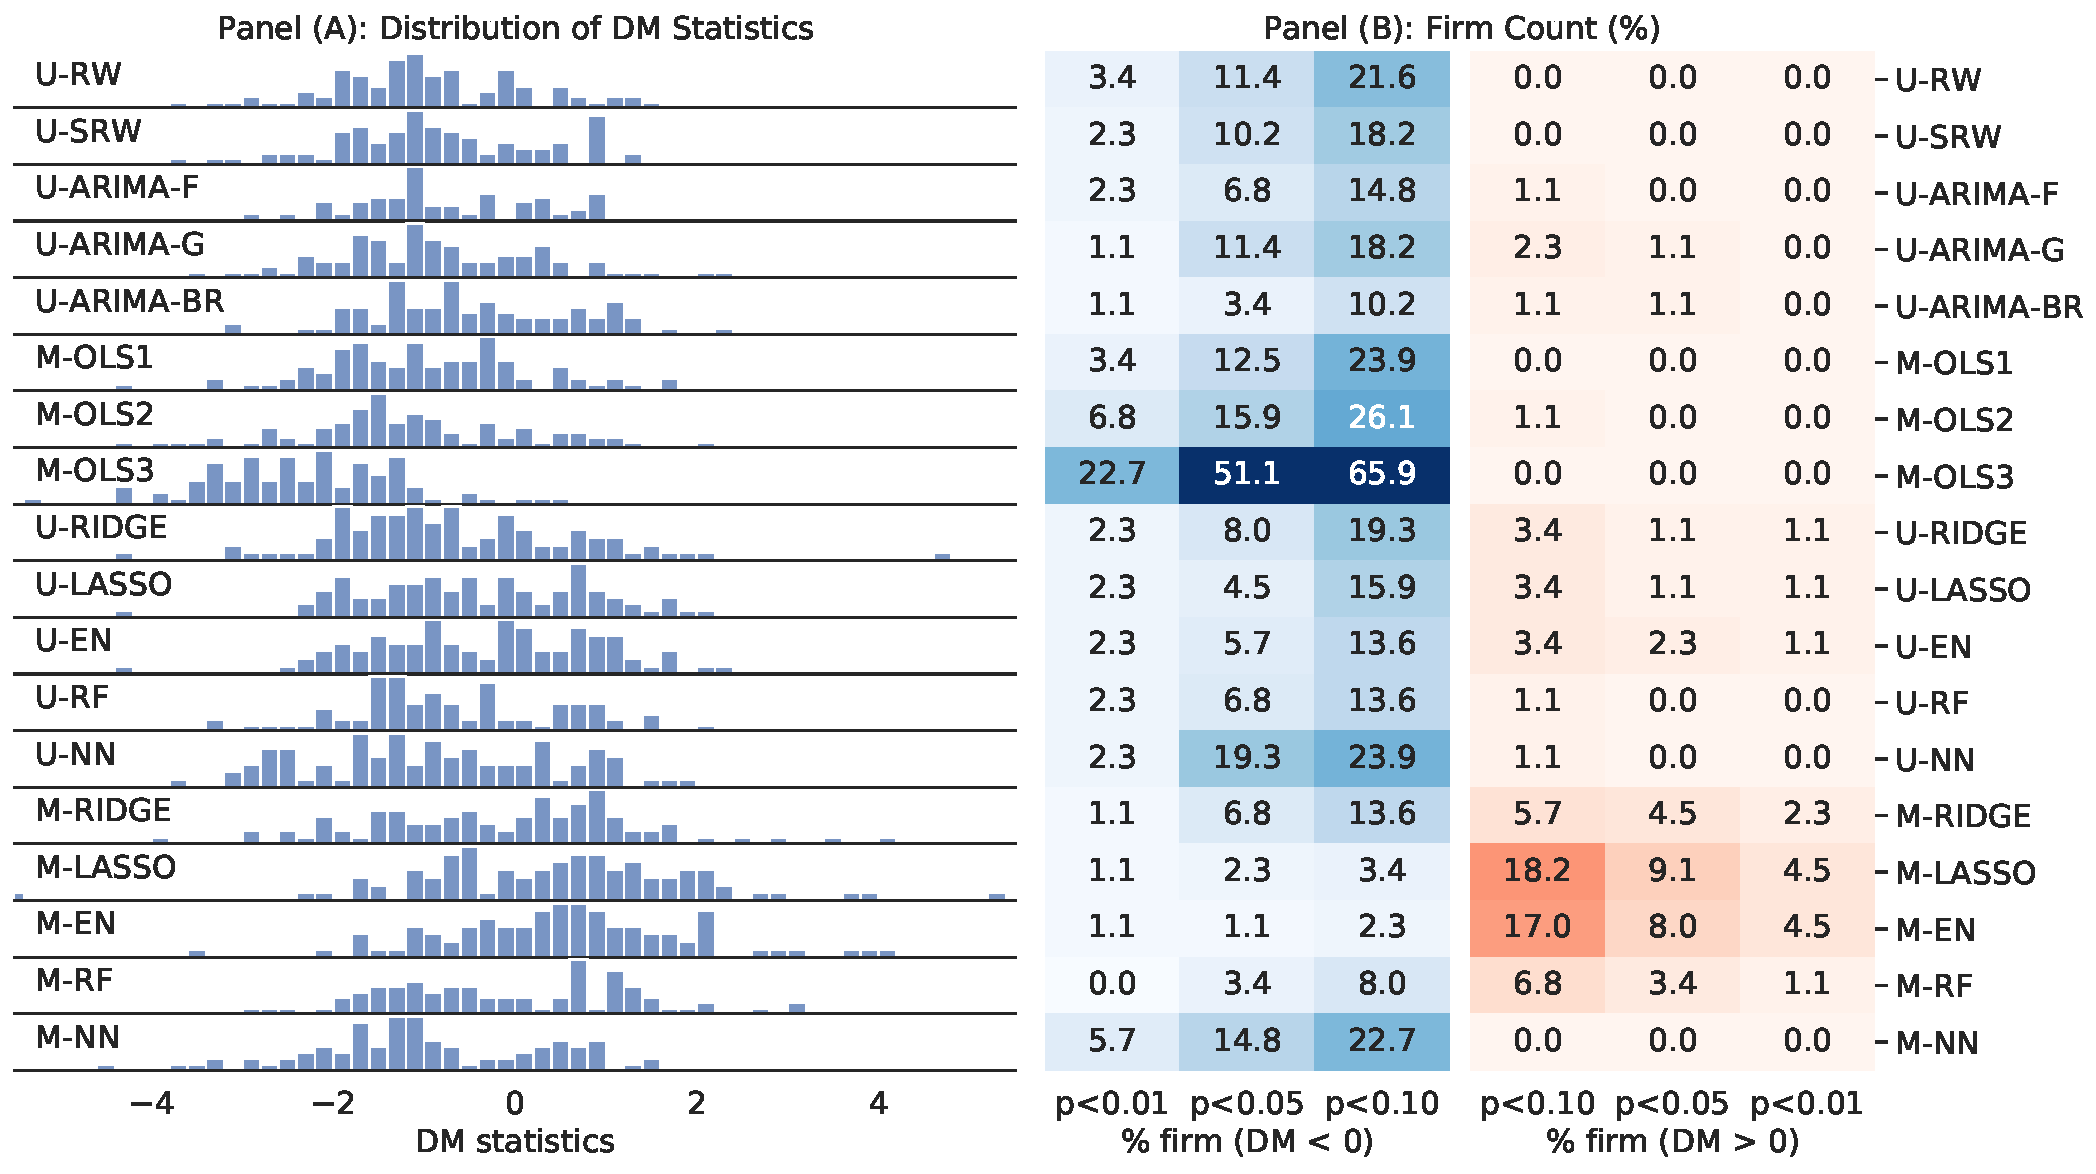
\includegraphics[width=\linewidth]{./img/_dm_MAPE_y_hat_ibes.pdf}
  \begin{threeparttable}
  \begin{tablenotes}
    \item[](注)各DM検定ではIBESをモデル1としており,損失関数はMAPEに対応するもの($L(e_t)=\left|\frac{e_t}{Y_t}\right|$)を用いている.Panel(A)はモデル2別の全88社のDM統計量の分布をヒストグラムで表している.Panel(B)は全88社のDM検定のうち,10\%,5\%,1\%の水準で統計的に有意な企業の割合(\%)をDM統計量の正負別に示したヒートマップである.色が濃いほど統計的に有意な企業の割合が大きいことを示している.
    \item[](出所)筆者作成.
  \end{tablenotes}
  \end{threeparttable}
\end{figure}

次に,損失関数をMAPEに対応するものとした両側DM検定を行い,図\ref{fig:dm_ibes_mape}にその結果をまとめている.表\ref{tab:acc_ibes}ではI/B/E/S業績予想と多変量機械学習アルゴリズムをMAPEで比較すると,I/B/E/S業績予想の方が小さい値であったが,図\ref{fig:dm_ibes_mape}.Panel(A)より,モデル2が多変量LASSO回帰とElastic Net回帰のときDM統計量が正の値に集中しており,図\ref{fig:dm_ibes_mape}.Panel(B)から,DM統計量が正の値で統計的に有意な企業の割合が多いことも確認できる(10\%,5\%,1\%水準で統計的に有意な企業の割合は,それぞれ約17~18\%,8~9\%,5\%).また,モデル2が多変量ランダムフォレスト回帰の場合はI/B/E/S業績予想と同程度の精度の予測を与えている.なお,損失関数をMSPEに対応するものとした両側DM検定でも同様な結果が得られ,多変量機械学習アルゴリズムはアナリスト予測と比べると統計的有意に精度が高い,もしくは精度の差がない予測を与える企業が多い結果となった.

通常,アナリストは本稿の時系列モデルが用いる情報(過去の四半期EPSの実績値や過去のファンダメンタル会計変数)以外にも広範囲の情報を反映した予測を行うと考えられるため\citep{sakurai1990},アナリスト予測は(多変量機械学習アルゴリズムも含めた)時系列モデルによる予測よりも精度が高いとされる.にもかかわらず,本稿のDM検定の結果から,多変量機械学習アルゴリズムはアナリスト予測と同等もしくはそれ以上に高い精度の予測を与えることが示された.

\part{予測の投資指標としての有用性} \label{par:portfolio}

最後に,本稿で推定した機械学習アルゴリズムによって得られた1期先四半期EPS予測の投資指標としての有用性について検証する.検証方法としては,代表的な投資指標である株価収益率を1期先四半期EPS予測値をもとに算出し,得られた株価予測収益率の高低によってロング・ショート・ポートフォリオを構築してどれくらいの超過リターンが得られるかを調べる.具体的には次のように行う.

\begin{enumerate}
  \item 時点$t-1$(各四半期の中間月末)において,株価$P_{t-1}$と1期先四半期EPS予測値$\hat{Y}_t$を用いて株価予測収益率$\frac{P_{t-1}}{\hat{Y}_t}$を全企業に対して計算する.
  % 現在の時点をtとすれば,1期先予測はt+1.でもモデルの表記と揃えるか.
  \item 全サンプル企業(時系列モデルは全1,003社,I/B/E/S業績予想は全88社)の株価予測収益率を降順にソートし,倍率順に1~5までの5つのポートフォリオを作成する.
  \item 高倍率企業で構成されるポートフォリオ1を空売りし,低倍率企業で構成されるポートフォリオ5を同じ額だけ買う.
  \item 1四半期(3ヶ月)保有し,ポートフォリオ1とポートフォリオ5のスプレッドを観測する.
\end{enumerate}

\noindent
以上のような操作を毎四半期行い,ポートフォリオを1四半期ごとにリバランスする.図\ref{fig:portfolio_return}は各予測手法に基づくロング・ショート・ポートフォリオ戦略の累積超過リターンを2018年8月末~2021年2月末まで示している.

\begin{figure}[tbp]
  \centering
  \caption{各予測手法に基づいたロング・ショート・ポートフォリオ戦略による累積超過リターン}
  \label{fig:portfolio_return}
  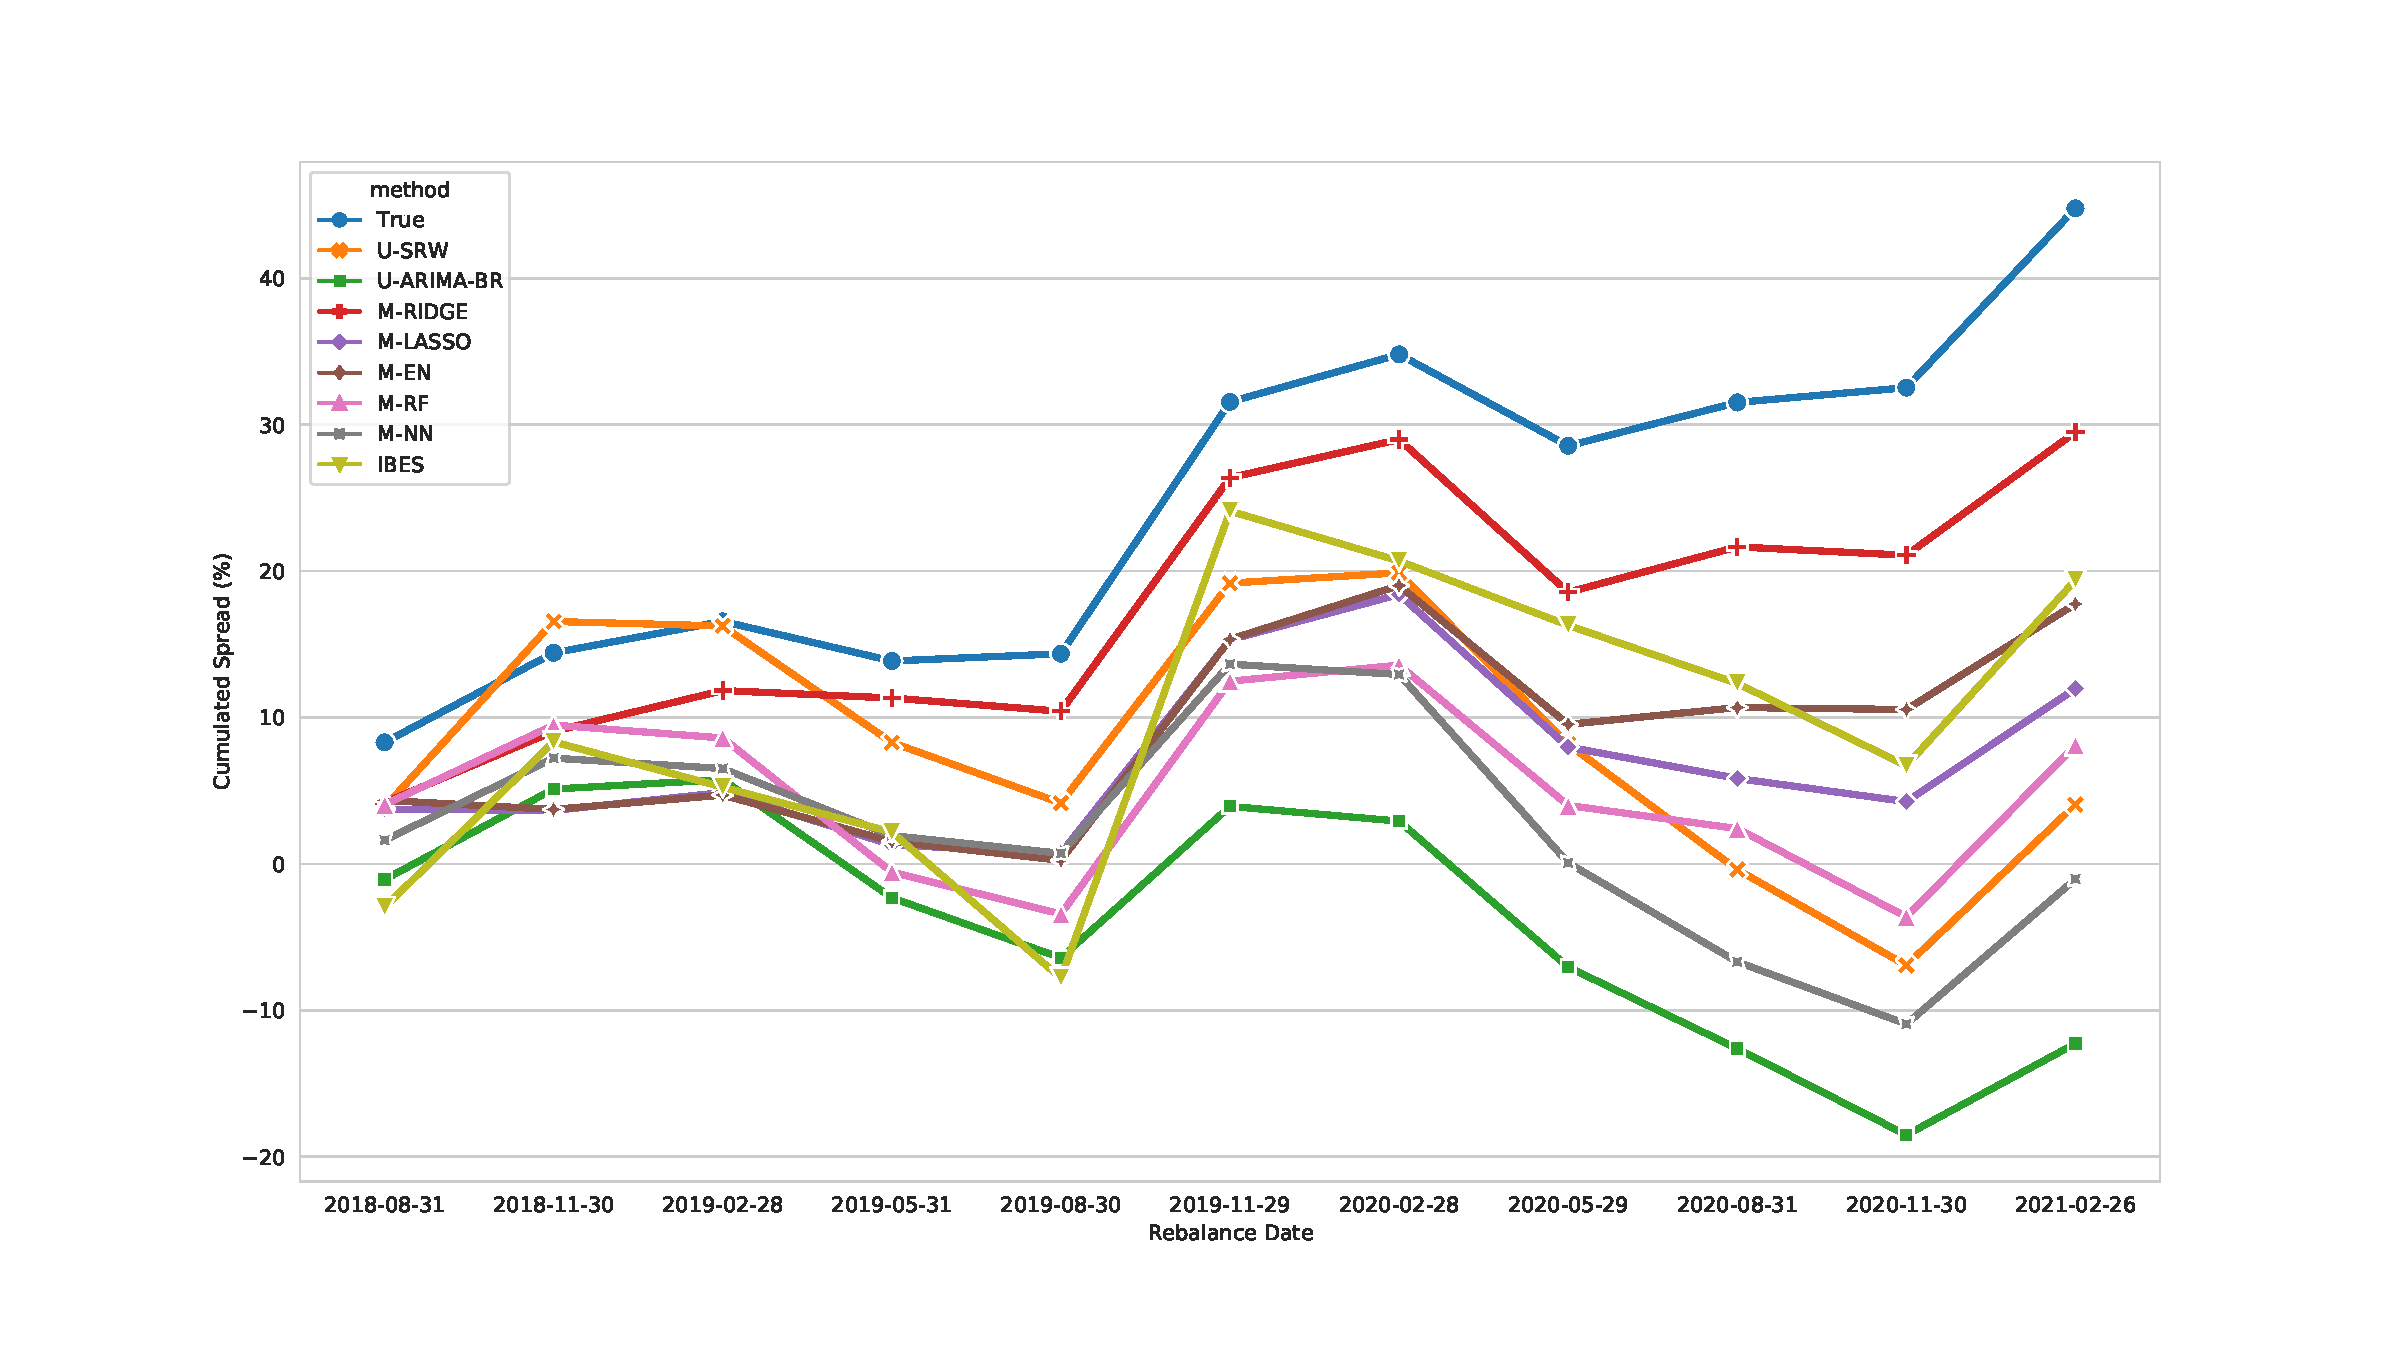
\includegraphics[width=\linewidth]{./img/_portfolio_return.pdf}
  \begin{threeparttable}
  \begin{tablenotes}
    \item[](注)リターン算出に用いた株価データは「日経NEEDS-FinancialQUEST」から収集している.Trueは株価予測収益率の算出に1期先四半期EPSの真の値を用いたときの超過リターンを示している.季節ランダムウオークモデル(U-SRW)は1年前の実績四半期EPSを用いた株価予測収益率を算出しているとみなすことができる.なお,株価予測収益率が負である企業は除外してポートフォリオを構築している.
    \item[](出所)筆者作成.
  \end{tablenotes}
  \end{threeparttable}
\end{figure}

まず,1期先四半期EPSの真の値をロング・ショート・ポートフォリオ戦略に用いると,プラスのリターンを獲得している.つまり,仮に1期前時点で次期四半期EPSを完璧に予測できるのであれば高い水準の超過リターンを得ることができることを意味する.各予測手法のうち,最も高いリターンを獲得したのは多変量Ridge回帰であり,最終時点の累積超過リターンは約30\%となった.次点でI/B/E/S業績予想が高いリターンを得ており,多変量Elastic Net回帰がそれをわずかに下回る結果となった.伝統的な線形時系列モデル(季節ランダムウオークモデル,\cite{brown1979univariate}のARIMAモデル)の超過リターンはいずれも低い水準の超過リターンであった.このように,機械学習アルゴリズム(特に多変量Ridge回帰)による予測には投資指標における有用性があることが確認された.

なお,I/B/E/S業績予想の超過リターンの標準偏差は12.2であり,他の時系列モデルの超過リターンの標準偏差(平均7.1)と比べると変動が大きいことがわかる.これは時系列モデルのサンプル企業が1,003社であるのに対し,I/B/E/S業績予想のカバレッジが88社と少数であるためリターンの変動が大きくなっていると考えられる.

\part{おわりに} \label{par:conclusion}

本稿では,機械学習アルゴリズムによる日本企業の四半期EPS予測を行い,伝統的な線形時系列モデルとの精度比較と,アナリスト予測との精度比較をそれぞれ行った.まず,機械学習アルゴリズムと伝統的な線形時系列モデルの予測精度を比較すると,単変量予測では予測精度に明らかな差は見られなかったが,多変量予測では,機械学習アルゴリズムの方が精度の高い予測を与えた.この結果から,機械学習アルゴリズムは,伝統的な線形時系列モデルでは捉えられない将来の四半期EPSとファンダメンタル会計変数の関係性を捉えることができ,機械学習アルゴリズムを用いることで日本企業のEPS予測のパフォーマンスを向上させる可能性が示唆される.次に,機械学習アルゴリズムとアナリストの予測精度を比較すると,前者は後者と同等もしくはそれ以上に高い精度の予測を与えることが明らかになった.具体的には,多変量NNの予測精度はアナリストより低いものの,多変量ランダムフォレスト回帰はアナリストと同程度で,多変量LASSO回帰,Elastic-Net回帰はアナリストよりも精度の高い予測を与えた.これにより,NN以外の機械学習アルゴリズムの日本企業の四半期EPS予測における有用性が示された.企業利益予測の研究分野では,長らく時系列モデルによる予測よりもアナリスト予測の方が適切であると暗黙裡に見なされてきたが,本稿の結果はその認識を覆すものとなった.さらに本稿の追加的な検証から,機械学習アルゴリズムによる四半期EPS予測値は投資指標としても優れており,多くの企業を予測対象とすることでより分散の効いた投資機会を得ることができると考えられる.

機械学習アルゴリズムはアナリスト以上に高い精度の予測を与えることに加え,予測プロセスが自動化されているため低コストであり,決算情報を公開する企業であれば全て予測対象とすることができる.\cite{yoneyama2010}によると日本企業のアナリストカバレッジは減少している傾向にあり,特に新興市場のカバー率は全体で10\%に満たないものとなっている.日本証券業協会はこうした事態に対処するため,「アナリストの中立性に配慮しつつ、新興市場に上場する企業のアナリストカバレッジを高める施策を検討する」という提言を行った\footnote{日本証券業協会「新興市場のあり方を考える委員会報告書」参照.}.しかし現実の問題としてアナリストは,重要顧客である機関投資家の保有比率が高く,株式売買が盛んで,売買手数料が大きい企業のみをカバーする傾向にあり\citep{nakai2006},市場で株式売買が少ない企業にアナリストの関心を引きつけることは困難で,費用対効果の問題も伴う.このような日本のアナリストカバレッジが限定的である現状に対し,機械学習アルゴリズムを用いることで,アナリストの関心を引かないような企業に対してもアナリストと同等もしくはそれ以上の精度の利益予測を低コストで提供できるであろう.

本稿の課題として,まず予測をより早い時点で実行できるようにすることが考えられる.本稿の予測のデザインは,前四半期決算情報の開示後,その情報をもとに1期先四半期EPSを予測するものとなっている.一方で,2期先,3期先のようにより早い時点で予測を行うことも十分に考えられる.その場合,予測に用いることができる情報集合を予測タイミング時点で利用可能なものに限定したうえで,複数期先予測の精度が保たれるのかを検証することが必要となるであろう.次に,過去の四半期EPSの実績値やファンダメンタル会計変数以外にも予測に用いることができる情報があるのかどうかを吟味することも挙げられる.本稿の予測で用いた説明変数は,公開された対象企業自身の会計データに限定しており,1企業内で完結しているものとなっている.しかし,企業の将来の利益を説明するものとして,マクロ要因や産業別要因,利害関係がある企業の情報なども考えられる.そのような対象企業外の情報の中から予測精度を向上させるものを模索することも有意義であろう.

機械学習アルゴリズムはハイパーパラメータ選択のプロセスやモデルの設定によって予測のパフォーマンスが大きく変動するため,本稿で得られた結果は必ずしも最良なものではないかもしれない.しかしながら,本稿の結果より,機械学習アルゴリズムはアナリストと比べて劣らない,もしくは優れた四半期EPS予測を与えることが明らかになった.このことから,現在日本で衰退してしまっている時系列モデルによる利益予測の研究が,機械学習アルゴリズムを用いることで再興する余地が十分にあることが示唆される.今後の研究で,統計的・機械的な手法による企業利益予測を更に発展させ,あらゆるステークホルダーに利用可能な幅広い企業の予測情報が提供されることを期待したい.

% 本稿の図表は全て筆者作成
% githubソースコード

% 参考文献
\newpage
\addcontentsline{toc}{section}{参考文献}
\bibliographystyle{jecon}
% https://www.eng.u-hyogo.ac.jp/faculty/hoshino/pc/tex_bibtex/
% http://mikilab.doshisha.ac.jp/dia/seminar/latex/doc/bib.html
% Harvard style
% \bibliographystyle{agsm}
% https://github.com/ShiroTakeda/jecon-bst
%%% BibTeX スタイルファイルの指定.jecon.bst を指定.
% \bibliographystyle{jplain}
\bibliography{ref}

% 付録
\newpage
% \addcontentsline{toc}{part}{付録}
\appendix

% \section{組み合わせ予測の結果} 
\section{} \label{app:comb}
本稿で扱った各時系列モデルの予測値系列をもとに,組み合わせ予測(算術平均)を算出する.

全時系列モデルの組み合わせ予測
\begin{equation}
\begin{split}
  \hat{Y}_t^{COMB-ALL} = \frac{1}{18} & \left( \hat{Y}_t^{RW} + \hat{Y}_t^{SRW} + \hat{Y}_t^{ARIMA-F} + \hat{Y}_t^{ARIMA-G} + \hat{Y}_t^{ARIMA-BR} \right. \\
  &+ \hat{Y}_t^{U-Ridge} + \hat{Y}_t^{U-LASSO} + \hat{Y}_t^{U-EN} + \hat{Y}_t^{U-RF} + \hat{Y}_t^{U-NN} \\
  &+ \hat{Y}_t^{OLS1} + \hat{Y}_t^{OLS2} + \hat{Y}_t^{OLS3} \\
  &\left. + \hat{Y}_t^{M-Ridge} + \hat{Y}_t^{M-LASSO} + \hat{Y}_t^{M-EN} + \hat{Y}_t^{M-RF} + \hat{Y}_t^{M-NN} \right)
\end{split}
\end{equation}

単変量モデルの組み合わせ予測
\begin{equation}
\begin{split}
\hat{Y}_t^{COMB-U} = \frac{1}{10} & \left( \hat{Y}_t^{RW} + \hat{Y}_t^{SRW} + \hat{Y}_t^{ARIMA-F} + \hat{Y}_t^{ARIMA-G} + \hat{Y}_t^{ARIMA-BR} \right. \\
&\left. + \hat{Y}_t^{U-Ridge} + \hat{Y}_t^{U-LASSO} + \hat{Y}_t^{U-EN} + \hat{Y}_t^{U-RF} + \hat{Y}_t^{U-NN} \right) \\
\end{split}
\end{equation}

単変量線形時系列モデルの組み合わせ予測
\begin{equation}
\begin{split}  
\hat{Y}_t^{COMB-U-TS} = \frac{1}{5} \left( \hat{Y}_t^{RW} + \hat{Y}_t^{SRW} + \hat{Y}_t^{ARIMA-F} + \hat{Y}_t^{ARIMA-G} + \hat{Y}_t^{ARIMA-BR} \right) \\
\end{split}
\end{equation}

単変量機械学習アルゴリズムの組み合わせ予測
\begin{equation}
\begin{split}  
\hat{Y}_t^{COMB-U-ML} = \frac{1}{5} \left( \hat{Y}_t^{U-Ridge} + \hat{Y}_t^{U-LASSO} + \hat{Y}_t^{U-EN} + \hat{Y}_t^{U-RF} + \hat{Y}_t^{U-NN} \right) \\
\end{split}
\end{equation}

多変量モデルの組み合わせ予測
\begin{equation}
\begin{split}  
\hat{Y}_t^{COMB-M} = \frac{1}{8} & \left( \hat{Y}_t^{OLS1} + \hat{Y}_t^{OLS2} + \hat{Y}_t^{OLS3} \right.\\
&\left. + \hat{Y}_t^{M-Ridge} + \hat{Y}_t^{M-LASSO} + \hat{Y}_t^{M-EN} + \hat{Y}_t^{M-RF} + \hat{Y}_t^{M-NN} \right) \\
\end{split}
\end{equation}

多変量線形回帰モデルの組み合わせ予測
\begin{equation}
\begin{split}  
\hat{Y}_t^{COMB-M-OLS} = \frac{1}{3} \left( \hat{Y}_t^{OLS1} + \hat{Y}_t^{OLS2} + \hat{Y}_t^{OLS3} \right) \\
\end{split}
\end{equation}

多変量機械学習アルゴリズムの組み合わせ予測
\begin{equation}
\begin{split}  
\hat{Y}_t^{COMB-M-ML} = \frac{1}{5} \left( \hat{Y}_t^{M-Ridge} + \hat{Y}_t^{M-LASSO} + \hat{Y}_t^{M-EN} + \hat{Y}_t^{M-RF} + \hat{Y}_t^{M-NN} \right) \\
\end{split}
\end{equation}

\noindent
表\ref{tab:acc_comb}は組み合わせ予測の各予測指標の全企業(1,003社)平均を四半期別と全予測期間で集計したものを示している.

\begin{landscape}
\begin{table}[tbp]
  % \centering
  \caption{組み合わせ予測による1期先四半期EPS予測の精度(1,003社平均)}
  \label{tab:acc_comb}
  % \small
  % %%% threeparttable %%%
\begin{threeparttable}[h]

% \begin{tabular}{lrrrrrrrrrrrrrrrrrrrr}
\begin{tabular}{lrrrp{1.5cm}rrrp{1.5cm}rrrp{1.5cm}rrrp{1.5cm}rrrp{1.5cm}}
% \begin{tabularx}{6cm}{lrrrXrrrXrrrXrrrXrrrX}

\toprule
{} & \multicolumn{4}{c}{Q1} & \multicolumn{4}{c}{Q2} & \multicolumn{4}{c}{Q3} & \multicolumn{4}{c}{Q4} & \multicolumn{4}{c}{Overall} \\
\cmidrule(lr){2-5}
\cmidrule(lr){6-9}
\cmidrule(lr){10-13}
\cmidrule(lr){14-17}
\cmidrule(lr){18-21}
% \tnote
{} &    MAE \tnote{b}&   MAPE \tnote{c}&   MSPE \tnote{d}& Large Forecast Error(\%) \tnote{e}&    MAE &   MAPE &   MSPE & Large Forecast Error(\%) &    MAE &   MAPE &   MSPE & Large Forecast Error(\%) &    MAE &   MAPE &   MSPE & Large Forecast Error(\%) &     MAE &   MAPE &   MSPE & Large Forecast Error(\%) \\
% \tnote
Model \tnote{a}     &        &        &        &                         &        &        &        &                         &        &        &        &                         &        &        &        &                         &         &        &        &                         \\
\midrule
U-RW       &   44.2 &  0.668 &  0.572 &                    42.6 &   27.6 &  0.529 &  0.408 &                    25.7 &   29.7 &  0.499 &  0.372 &                    22.3 &   47.9 &  0.621 &  0.514 &                    36.1 &    37.3 &  0.579 &  0.467 &                    31.7 \\
U-SRW      &   27.1 &  0.547 &  0.436 &                    27.8 &   27.4 &  0.505 &  0.390 &                    23.8 &   26.3 &  0.461 &  0.338 &                    20.4 &   47.2 &  0.573 &  0.464 &                    32.2 &    32.0 &  0.521 &  0.407 &                    26.0 \\
U-ARIMA-F  &   32.6 &  0.549 &  0.437 &                    29.5 &   25.7 &  0.480 &  0.362 &                    22.4 &   28.3 &  0.477 &  0.355 &                    21.4 &   46.7 &  0.573 &  0.463 &                    32.3 &    33.3 &  0.520 &  0.404 &                    26.4 \\
U-ARIMA-G  &   37.7 &  0.567 &  0.460 &                    32.4 &   30.9 &  0.481 &  0.366 &                    23.9 &   33.2 &  0.488 &  0.370 &                    23.5 &   50.2 &  0.570 &  0.461 &                    31.8 &    38.0 &  0.526 &  0.414 &                    27.9 \\
U-ARIMA-BR &   36.4 &  0.559 &  0.445 &                    29.3 &   29.2 &  0.482 &  0.362 &                    22.5 &   30.1 &  0.471 &  0.348 &                    21.0 &   47.7 &  0.564 &  0.452 &                    30.1 &    35.8 &  0.519 &  0.402 &                    25.7 \\
M-OLS1     &   64.1 &  0.626 &  0.527 &                    38.8 &   50.6 &  0.556 &  0.447 &                    32.0 &   40.4 &  0.528 &  0.414 &                    27.4 &   60.9 &  0.603 &  0.499 &                    35.4 &    54.0 &  0.578 &  0.472 &                    33.4 \\
M-OLS2     &   62.5 &  0.613 &  0.514 &                    38.0 &   44.0 &  0.549 &  0.439 &                    30.8 &   77.5 &  0.569 &  0.461 &                    32.4 &   84.4 &  0.625 &  0.526 &                    38.6 &    67.1 &  0.589 &  0.485 &                    35.0 \\
M-OLS3     &  333.8 &  0.821 &  0.769 &                    67.9 &  278.6 &  0.798 &  0.738 &                    63.8 &  263.9 &  0.790 &  0.727 &                    62.0 &  225.4 &  0.797 &  0.733 &                    62.7 &   275.4 &  0.801 &  0.742 &                    64.1 \\
U-RIDGE    &   41.9 &  0.576 &  0.469 &                    33.5 &   35.4 &  0.506 &  0.391 &                    26.2 &   37.0 &  0.499 &  0.373 &                    22.2 &   49.7 &  0.575 &  0.464 &                    31.5 &    41.0 &  0.539 &  0.424 &                    28.3 \\
U-LASSO    &   35.2 &  0.591 &  0.474 &                    28.9 &   31.0 &  0.530 &  0.401 &                    21.6 &   33.9 &  0.521 &  0.385 &                    18.4 &   45.5 &  0.592 &  0.473 &                    27.9 &    36.4 &  0.559 &  0.433 &                    24.2 \\
U-EN       &   34.0 &  0.581 &  0.462 &                    28.4 &   30.7 &  0.519 &  0.390 &                    21.4 &   32.7 &  0.510 &  0.372 &                    17.7 &   45.6 &  0.591 &  0.471 &                    27.6 &    35.7 &  0.550 &  0.423 &                    23.8 \\
U-RF       &   27.1 &  0.548 &  0.435 &                    28.8 &   25.0 &  0.480 &  0.358 &                    22.2 &   26.6 &  0.464 &  0.338 &                    19.2 &   40.8 &  0.561 &  0.445 &                    29.1 &    29.9 &  0.513 &  0.394 &                    24.8 \\
U-NN       &   50.7 &  0.624 &  0.515 &                    34.4 &   49.4 &  0.580 &  0.460 &                    28.2 &   49.4 &  0.554 &  0.430 &                    25.7 &   60.5 &  0.626 &  0.516 &                    34.0 &    52.5 &  0.596 &  0.480 &                    30.6 \\
M-RIDGE    &   38.1 &  0.527 &  0.419 &                    29.3 &   33.9 &  0.483 &  0.374 &                    25.1 &   36.6 &  0.468 &  0.355 &                    24.2 &   45.7 &  0.534 &  0.429 &                    30.3 &    38.6 &  0.503 &  0.394 &                    27.2 \\
M-LASSO    &   23.6 &  0.490 &  0.374 &                    23.1 &   23.5 &  0.438 &  0.321 &                    19.1 &   24.3 &  0.422 &  0.302 &                    17.2 &   38.1 &  0.495 &  0.382 &                    24.4 &    27.4 &  0.461 &  0.345 &                    21.0 \\
M-EN       &   22.9 &  0.479 &  0.362 &                    21.8 &   22.7 &  0.425 &  0.308 &                    18.2 &   23.7 &  0.417 &  0.296 &                    16.8 &   37.7 &  0.492 &  0.377 &                    23.7 &    26.8 &  0.453 &  0.336 &                    20.1 \\
M-RF       &   24.7 &  0.495 &  0.382 &                    25.7 &   21.2 &  0.413 &  0.295 &                    17.9 &   22.7 &  0.408 &  0.287 &                    17.2 &   36.8 &  0.513 &  0.398 &                    25.8 &    26.3 &  0.457 &  0.340 &                    21.7 \\
M-NN       &   35.8 &  0.588 &  0.480 &                    33.7 &   36.8 &  0.534 &  0.416 &                    27.1 &   33.0 &  0.517 &  0.392 &                    23.4 &   46.4 &  0.595 &  0.485 &                    33.4 &    38.0 &  0.558 &  0.443 &                    29.4 \\
\bottomrule
\end{tabular}

%%% table footnote %%%
\begin{tablenotes}
\item[a] 各モデルの先頭文字列U-は単変量モデル, M-は多変量モデルを表す. また, RWはランダムウオークモデル, SRWは季節ランダムウオークモデル, ARIMA-F, ARIMA-G, ARIMA-BRはそれぞれ\cite*{foster1977quarterly, griffin1977time, brown1979univariate}の設定のARIMAモデル, OLS1, OLS2, OLS3はそれぞれ式(\ref{eq:ols1}), 式(\ref{eq:ols2}), 式(\ref{eq:ols3})の線形回帰モデル, RIDGEはRidge回帰モデル, LASSOはLASSO回帰モデル, ENはElastic Net回帰モデル, RFはランダムフォレスト回帰モデル, NNはニューラルネットワークモデルを表す.
\item[b] 平均絶対誤差(Mean Absolute Error: MAE)
\item[c] 平均絶対誤差率(Mean Absolute Percentage Error: MAPE)
\item[d] 平均二乗誤差率(Mean Squared Percentage Error: MSPE)
\item[e] 絶対予測誤差率$\left| \frac{Y_t -{\hat Y}_t}{Y_t} \right|$が1を超えるLarge Forecast Errorサンプルについては絶対予測誤差率を1としており, 表に全予測サンプルに占めるLarge Forecast Errorサンプルの割合(\%)を示している.
\end{tablenotes}
\end{threeparttable}  
  \scalebox{0.75}[0.75]{
    %%% threeparttable %%%
\begin{threeparttable}

% \begin{tabular}{lrrrrrrrrrrrrrrrrrrrr}
\begin{tabular}{lrrrp{1.5cm}rrrp{1.5cm}rrrp{1.5cm}rrrp{1.5cm}rrrp{1.5cm}}
% \begin{tabularx}{6cm}{lrrrXrrrXrrrXrrrXrrrX}

\toprule
{} & \multicolumn{4}{c}{Q1} & \multicolumn{4}{c}{Q2} & \multicolumn{4}{c}{Q3} & \multicolumn{4}{c}{Q4} & \multicolumn{4}{c}{Overall} \\
\cmidrule(lr){2-5}
\cmidrule(lr){6-9}
\cmidrule(lr){10-13}
\cmidrule(lr){14-17}
\cmidrule(lr){18-21}
% \tnote
{} &    MAE \tnote{b}&   MAPE \tnote{c}&   MSPE \tnote{d}& Large Forecast Error(\%) \tnote{e}&    MAE &   MAPE &   MSPE & Large Forecast Error(\%) &    MAE &   MAPE &   MSPE & Large Forecast Error(\%) &    MAE &   MAPE &   MSPE & Large Forecast Error(\%) &     MAE &   MAPE &   MSPE & Large Forecast Error(\%) \\
% \tnote
Model \tnote{a}     &        &        &        &                         &        &        &        &                         &        &        &        &                         &        &        &        &                         &         &        &        &                         \\
\midrule

COMB-ALL   &   38.0 &  0.554 &  0.447 &                    31.5 &   30.4 &  0.479 &  0.365 &                    24.5 &   31.5 &  0.473 &  0.353 &                    22.3 &   44.0 &  0.551 &  0.438 &                    29.6 &    36.0 &  0.514 &  0.401 &                    27.0 \\
COMB-U &   29.5 &  0.548 &  0.435 &                    29.1 &   25.7 &  0.471 &  0.345 &                    20.1 &   26.6 &  0.454 &  0.329 &                    19.1 &   41.7 &  0.554 &  0.439 &                    28.8 &    30.9 &  0.507 &  0.387 &                    24.3 \\
COMB-U-TS  &   29.8 &  0.549 &  0.438 &                    30.0 &   24.0 &  0.460 &  0.338 &                    20.3 &   25.7 &  0.457 &  0.336 &                    20.3 &   42.9 &  0.552 &  0.439 &                    29.3 &    30.6 &  0.504 &  0.388 &                    25.0 \\
COMB-U-ML  &   34.1 &  0.565 &  0.452 &                    30.7 &   30.6 &  0.502 &  0.374 &                    22.9 &   31.4 &  0.484 &  0.350 &                    19.4 &   45.1 &  0.576 &  0.458 &                    29.5 &    35.3 &  0.532 &  0.408 &                    25.6 \\
COMB-M &   58.5 &  0.590 &  0.487 &                    35.4 &   47.2 &  0.533 &  0.429 &                    31.0 &   46.9 &  0.518 &  0.407 &                    27.9 &   55.0 &  0.576 &  0.471 &                    33.8 &    51.9 &  0.554 &  0.448 &                    32.0 \\
COMB-M-OLS &  130.0 &  0.698 &  0.619 &                    50.8 &  106.7 &  0.658 &  0.569 &                    45.2 &  101.6 &  0.650 &  0.556 &                    42.2 &  102.3 &  0.680 &  0.592 &                    46.8 &   110.1 &  0.671 &  0.584 &                    46.2 \\
COMB-M-ML  &   24.2 &  0.487 &  0.371 &                    23.1 &   23.2 &  0.421 &  0.305 &                    18.9 &   23.0 &  0.407 &  0.287 &                    17.0 &   36.2 &  0.499 &  0.385 &                    25.1 &    26.7 &  0.454 &  0.337 &                    21.0 \\

% Number of Forecasts     & \multicolumn{4}{c}{N=3,009} & \multicolumn{4}{c}{N=3,009} & \multicolumn{4}{c}{N=3,009} & \multicolumn{4}{c}{N=3,009} & \multicolumn{4}{c}{N=12,036} \\
\# of Forecasts     & \multicolumn{4}{c}{N=3,009} & \multicolumn{4}{c}{N=3,009} & \multicolumn{4}{c}{N=3,009} & \multicolumn{4}{c}{N=3,009} & \multicolumn{4}{c}{N=12,036} \\
\bottomrule
\end{tabular}

%%% table footnote %%%
\begin{tablenotes}
\item[a] COMB-ALLは全時系列モデル,COMB-Uは単変量モデル,COMB-U-TSは単変量線形時系列モデル,COMB-U-MLは単変量機械学習アルゴリズム,COMB-Mは多変量モデル,COMB-M-OLSは多変量線形回帰モデル,COMB-M-MLは多変量機械学習アルゴリズムの組み合わせ予測を表す.
\item[b] 平均絶対誤差(Mean Absolute Error: MAE)
\item[c] 平均絶対誤差率(Mean Absolute Percentage Error: MAPE)
\item[d] 平均二乗誤差率(Mean Squared Percentage Error: MSPE)
\item[e] 絶対予測誤差率$\left| \frac{Y_t -{\hat Y}_t}{Y_t} \right|$が1を超えるLarge Forecast Errorサンプルについては絶対予測誤差率を1としており, 全予測サンプルに占めるLarge Forecast Errorサンプルの割合(\%)を示している.
\item[] (出所)筆者作成.
\end{tablenotes}
\end{threeparttable}  
  }
\end{table}
\end{landscape}

\newpage
% \section{全企業(1,003社)のDM検定のDM検定量の分布(全通り)} 
\section{} \label{app:dm}
モデル1とモデル2の組合せ全通りにおける全1,003社のDM統計量の分布を図\ref{fig:dm_all}に示している.なお,DM検定で用いた損失関数はMAEに対応したものである.MAE以外の精度指標,MAPE,MSPEに対応する損失関数を用いたDM統計量の分布は,GitHubに掲載している\footnote{GitHubソースコード \url{https://github.com/hessihan/eps_foracasting}}.

\begin{figure}[hbtp]
  \centering
  \caption{全企業(1,003社)のDM統計量の分布(loss: MAE)}
  \label{fig:dm_all}
  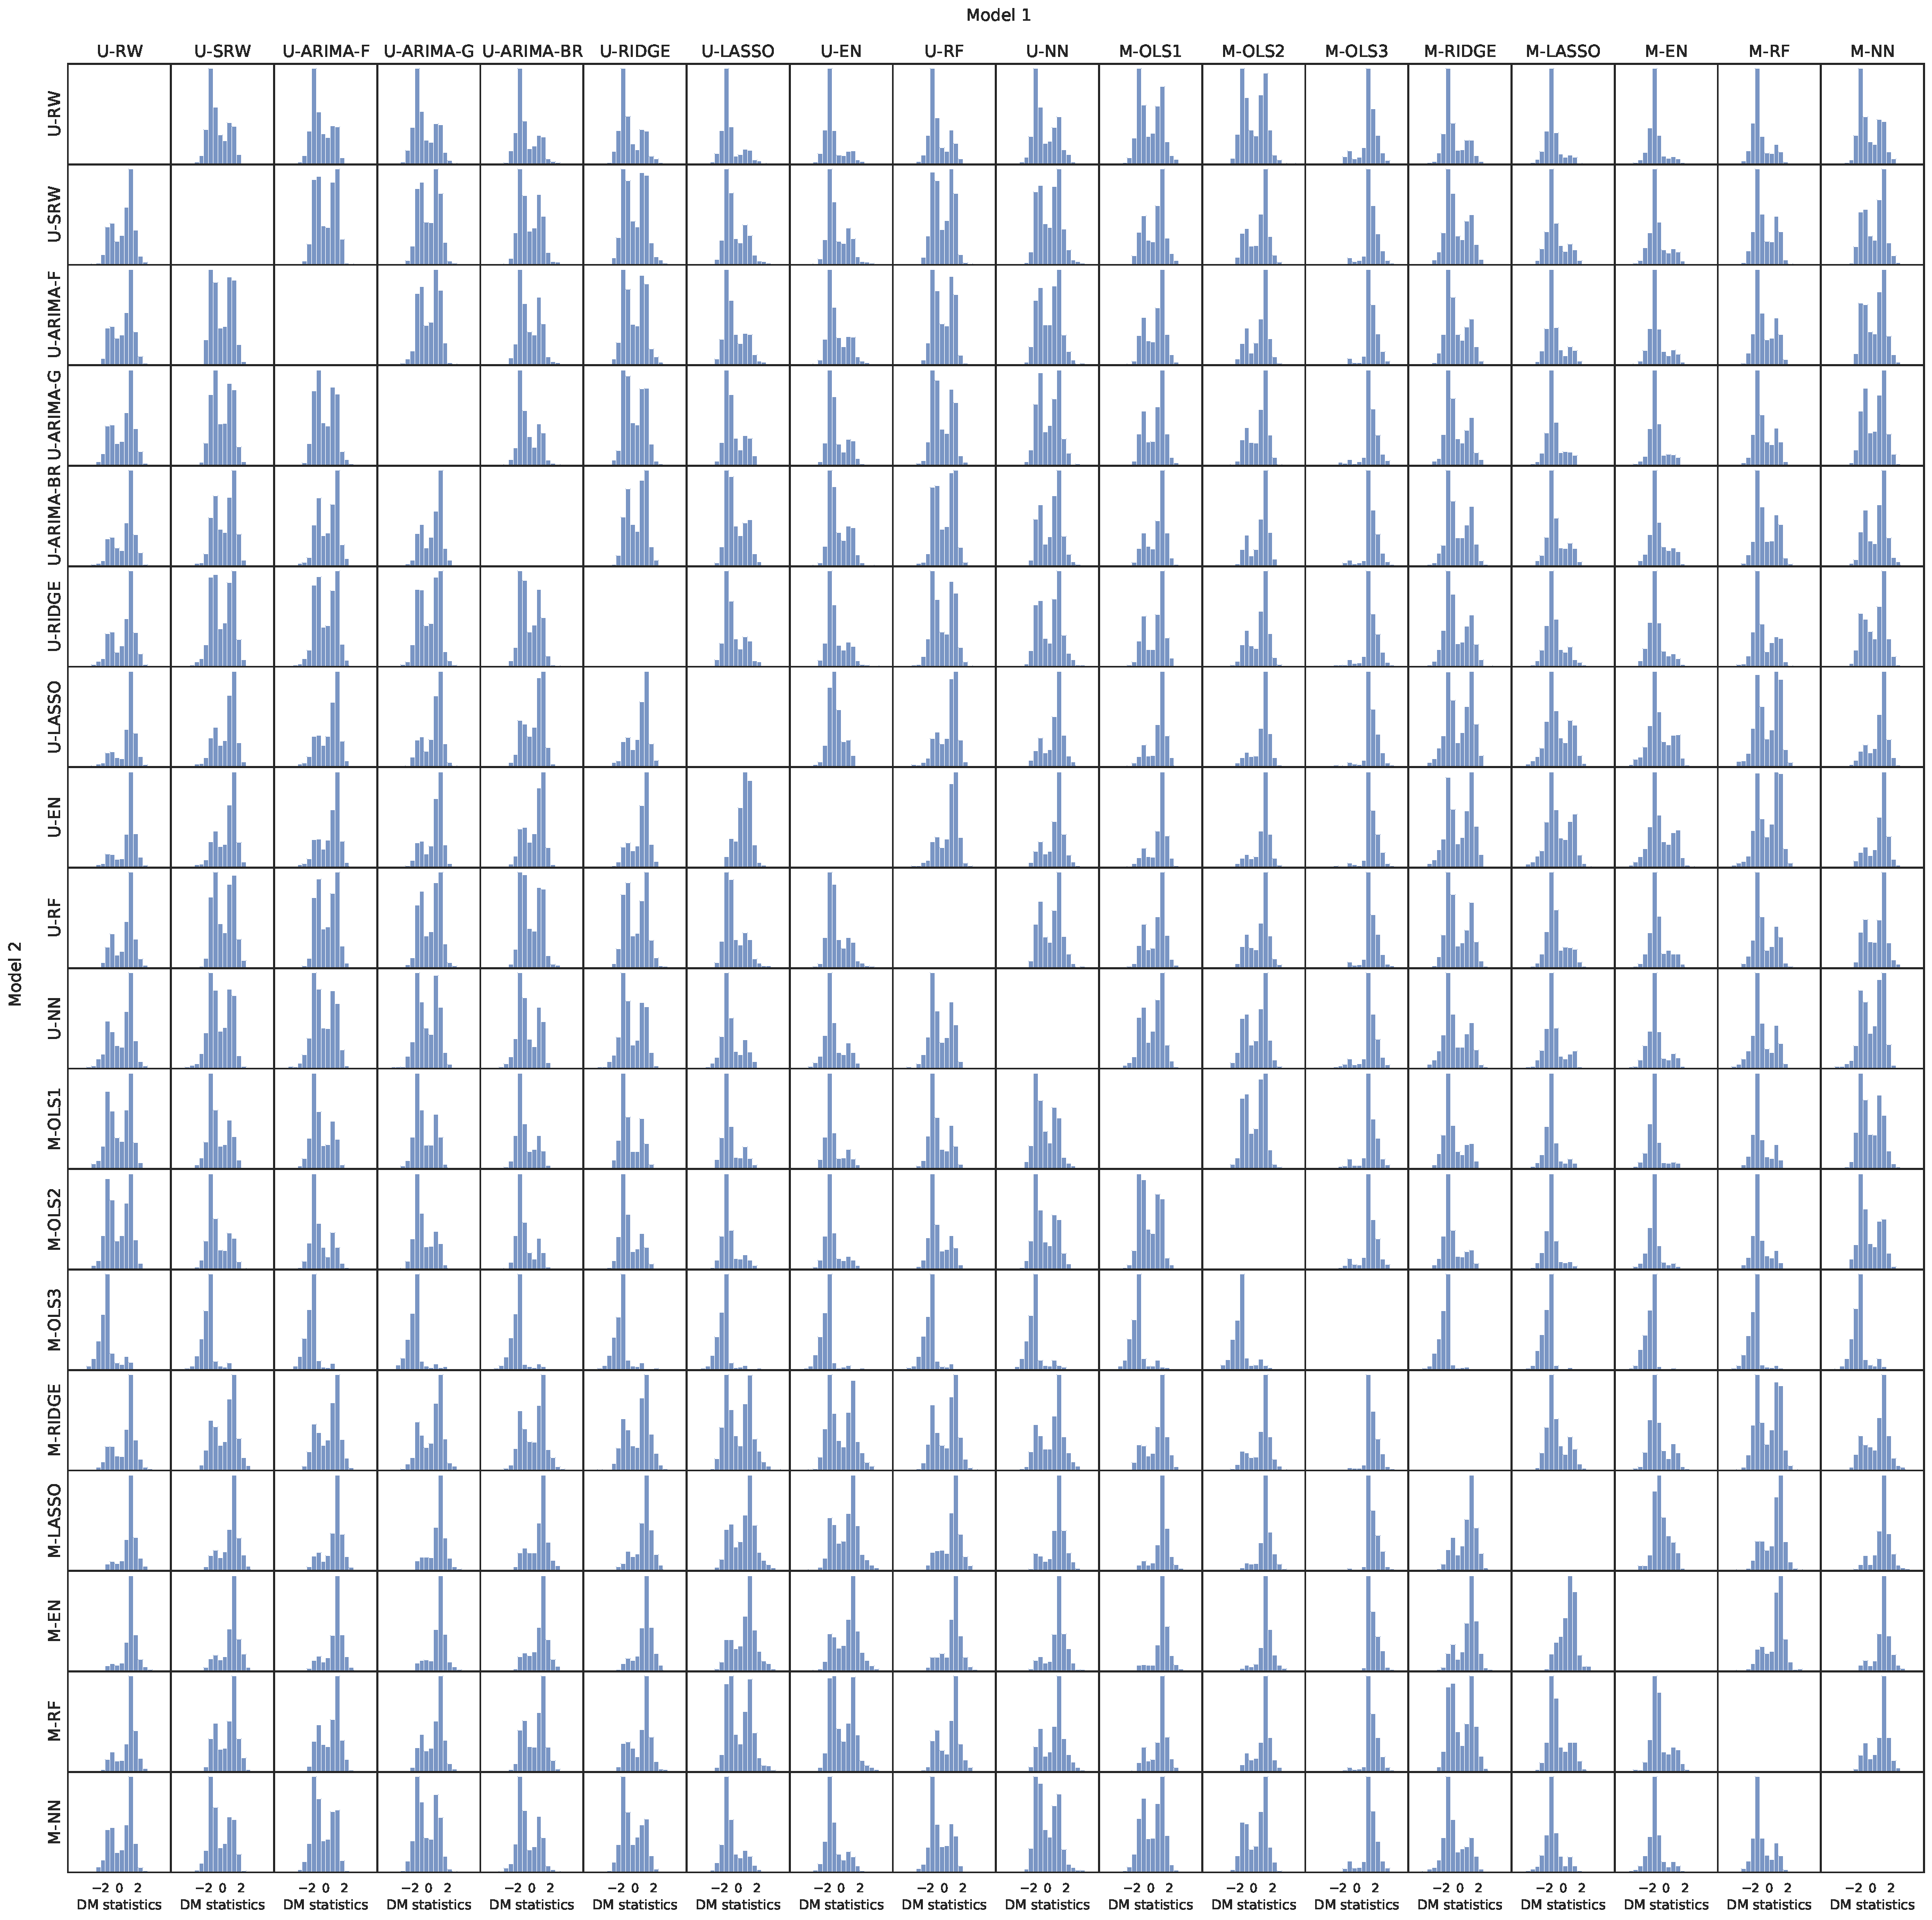
\includegraphics[width=\linewidth]{./img/_dm_mat_MAE.pdf}
  \begin{threeparttable}
  \begin{tablenotes}
    \item[](出所)筆者作成.
  \end{tablenotes}
  \end{threeparttable}  
\end{figure}

\newpage
% \section{企業別予測精度(MAE)} 
\section{} \label{app:acc_by_firm}
全予測期間で集計した各企業別のMAEを表\ref{tab:mae_by_firm}に示している.なお,1企業あたり同じ構造のモデルをローリングサンプルごとに12回推定し,得られた12個の予測値に基づいてMAEを計算している(第\ref{par:model}部\ref{sec:rolling}節参照).他の精度指標についても同様に算出し,GitHubに掲載している.なお,各モデルの先頭文字列U-は単変量モデル,M-は多変量モデルを表す. また,RWはランダムウオーク,SRWは季節ランダムウオーク,F,G,BRはそれぞれ\cite*{foster1977quarterly, griffin1977time, brown1979univariate}のARIMAモデル,OLS1,OLS2,OLS3はそれぞれ式(\ref{eq:ols1}),式(\ref{eq:ols2}),式(\ref{eq:ols3})の線形回帰モデル,RIDはRidge回帰,LASはLASSO回帰,ENはElastic Net回帰,RFはランダムフォレスト回帰,NNはニューラルネットワークを表す.

%
%===================================================
% longtable のサンプル   dcolumn も使っている
%===================================================
\tiny
% \begin{longtable}[c]{llllllllllllllllllll}
\begin{longtable}[c]{lp{3mm}p{3mm}p{3mm}p{3mm}p{3mm}p{3mm}p{3mm}p{3mm}p{3mm}p{3mm}p{3mm}p{3mm}p{3mm}p{3mm}p{3mm}p{3mm}p{3mm}p{3mm}p{3mm}}
\caption{企業別予測精度(MAE)}
\label{tab:mae_by_firm}
\\
%------ 最初のページの表の最上部 ----
\toprule
% Model &   U-RW &  U-SRW & U-ARIMA-F & U-ARIMA-G & U-ARIMA-BR &  M-OLS1 &  M-OLS2 &   M-OLS3 & U-RIDGE & U-LASSO &   U-EN &   U-RF &    U-NN & M-RIDGE & M-LASSO &   M-EN &   M-RF &    M-NN &   IBES \\
% Firm            &        &        &           &           &            &         &         &          &         &         &        &        &         &         &         &        &        &         &        \\
Model &   U-RW &  U-SRW & U-F & U-G & U-BR &  M-OLS1 &  M-OLS2 &   M-OLS3 & U-RID & U-LAS &   U-EN &   U-RF &    U-NN & M-RID & M-LAS &   M-EN &   M-RF &    M-NN &   IBES \\
Firm            &        &        &           &           &            &         &         &          &         &         &        &        &         &         &         &        &        &         &        \\
\midrule
\endfirsthead
%------ 2ページ以降の表の最上部 ----
\toprule
% Model &   U-RW &  U-SRW & U-ARIMA-F & U-ARIMA-G & U-ARIMA-BR &  M-OLS1 &  M-OLS2 &   M-OLS3 & U-RIDGE & U-LASSO &   U-EN &   U-RF &    U-NN & M-RIDGE & M-LASSO &   M-EN &   M-RF &    M-NN &   IBES \\
% Firm            &        &        &           &           &            &         &         &          &         &         &        &        &         &         &         &        &        &         &        \\
Model &   U-RW &  U-SRW & U-F & U-G & U-BR &  M-OLS1 &  M-OLS2 &   M-OLS3 & U-RID & U-LAS &   U-EN &   U-RF &    U-NN & M-RID & M-LAS &   M-EN &   M-RF &    M-NN &   IBES \\
Firm            &        &        &           &           &            &         &         &          &         &         &        &        &         &         &         &        &        &         &        \\
\midrule
\endhead
%----- ページの表の最下部 --------
\bottomrule
\endfoot
%----- 最終ページの表の最下部 --------
\bottomrule
\endlastfoot
%----------------------------------------------------------------
あらた             &   30.6 &   17.9 &      19.2 &      18.7 &       19.7 &    20.5 &    29.5 &     94.4 &    17.3 &    16.8 &   21.4 &   19.5 &    15.7 &    19.6 &    17.5 &   17.5 &   20.9 &    26.4 &      - \\
いすゞ自動車          &   22.8 &   10.0 &      10.8 &      14.4 &       11.8 &    21.8 &    10.4 &     71.0 &    13.1 &    13.8 &   13.8 &   13.4 &    12.5 &     7.9 &     8.1 &    8.0 &   11.3 &    16.6 &   10.0 \\
いなげや            &   18.4 &   18.0 &      16.4 &      16.7 &       13.8 &    21.9 &    17.4 &     24.6 &    16.7 &    15.7 &   15.8 &   18.1 &    22.6 &    14.6 &    15.7 &   15.0 &   11.4 &    21.2 &      - \\
かどや製油           &   34.9 &   22.7 &      23.2 &      23.8 &       25.4 &    34.4 &    23.3 &     84.6 &    24.5 &    30.4 &   30.4 &   26.9 &    34.8 &    27.5 &    40.0 &   40.0 &   22.0 &    31.4 &      - \\
きんでん            &   26.6 &    3.6 &       3.7 &       4.0 &        3.9 &     5.4 &     7.6 &     15.1 &     4.4 &     4.3 &    4.3 &    3.6 &     7.8 &     3.0 &     2.3 &    2.3 &    5.0 &     7.3 &      - \\
さくらインターネット      &    2.2 &    2.8 &       2.4 &      67.9 &       57.0 &   145.0 &    65.9 &    264.1 &    62.6 &    62.4 &   62.4 &    2.6 &   122.3 &     3.1 &     5.8 &    5.8 &   12.3 &   415.0 &      - \\
たけびし            &    6.8 &   10.3 &       9.0 &       9.1 &        8.3 &    10.8 &    10.2 &     20.0 &     7.7 &    10.0 &    8.5 &    7.2 &     7.2 &     6.0 &     3.8 &    3.9 &    7.5 &    11.8 &      - \\
なとり             &   45.4 &   11.1 &      11.4 &      10.0 &        9.1 &    12.0 &    13.8 &     40.8 &    11.5 &    12.3 &   12.3 &    8.6 &     9.2 &     5.6 &     4.0 &    4.0 &   10.1 &    12.8 &      - \\
はせがわ            &   24.3 &   14.2 &      13.4 &      13.3 &       12.2 &    20.3 &    14.6 &     28.5 &    16.3 &    16.3 &   17.8 &   12.7 &    20.0 &     4.8 &     4.4 &    3.4 &    9.9 &    14.7 &      - \\
はるやまホールディングス    &   47.0 &   47.0 &      43.3 &      31.8 &       36.6 &    43.6 &    33.9 &    137.6 &    45.2 &    49.1 &   49.1 &   46.6 &    39.1 &    31.1 &    28.5 &   27.1 &   34.8 &    28.8 &      - \\
ぴあ              &   40.9 &   49.1 &      35.5 &      34.7 &       45.0 &    38.2 &    43.2 &    183.8 &    39.8 &    33.9 &   33.9 &   36.3 &    41.0 &    25.4 &    29.1 &   32.4 &   39.4 &    47.8 &      - \\
りらいあコミュニケーションズ  &   33.0 &   32.6 &      44.6 &      56.0 &       46.1 &    39.1 &    81.1 &    464.1 &    46.3 &    26.1 &   26.1 &   20.5 &    34.1 &    45.4 &    26.1 &   26.1 &   22.4 &    36.3 &      - \\
わかもと製薬          &   13.4 &    9.0 &       9.6 &       9.4 &        7.7 &    10.5 &    10.2 &     20.9 &     8.8 &     8.3 &    8.3 &   12.2 &    13.2 &     8.1 &     8.3 &    8.3 &    9.4 &    10.0 &      - \\
アイカ工業           &   11.0 &    9.6 &       8.8 &       8.6 &        7.4 &     9.1 &     9.3 &     11.4 &     9.6 &    14.2 &   10.7 &    8.7 &    11.6 &     7.6 &     7.5 &    7.4 &    8.1 &    22.5 &      - \\
アイコム            &   41.9 &   15.3 &      15.6 &      21.7 &       20.6 &    23.3 &    26.7 &     81.8 &    18.4 &    18.4 &   18.4 &   16.1 &    22.5 &    24.8 &    18.0 &   16.6 &   18.0 &    19.8 &      - \\
アイシン            &   71.9 &  106.9 &     102.7 &     128.4 &      116.8 &   112.1 &   127.3 &    201.5 &    87.1 &    85.7 &   85.7 &   85.3 &    92.7 &    54.1 &    49.1 &   45.9 &   77.4 &   103.3 &   68.9 \\
アイダエンジニアリング     &   10.7 &    7.1 &       6.1 &       7.4 &        7.6 &    10.8 &     9.1 &     42.3 &     8.6 &     8.5 &    8.5 &    6.8 &     5.5 &     9.5 &     7.6 &    7.6 &    7.5 &     6.2 &      - \\
アイチコーポレーション     &   10.8 &    6.0 &       6.3 &       6.2 &        5.8 &     5.8 &     5.9 &     17.9 &     5.7 &     7.6 &    6.2 &    6.9 &     7.7 &     3.7 &     2.6 &    3.2 &    2.6 &     5.2 &      - \\
アイティフォー         &   10.3 &    2.9 &       2.9 &       2.2 &        2.5 &     3.2 &     3.1 &     21.4 &     4.1 &     3.4 &    3.2 &    3.6 &     5.2 &     1.9 &     1.5 &    1.7 &    2.3 &     5.1 &      - \\
アイティメディア        &    3.0 &    4.4 &       3.3 &       2.6 &        3.6 &    11.7 &    11.5 &     13.5 &     6.8 &     6.8 &    7.0 &    3.7 &    11.9 &     2.6 &     3.3 &    2.9 &    3.2 &     6.5 &      - \\
アイネス            &   49.0 &   47.0 &      49.3 &      43.7 &       42.0 &    54.8 &    41.2 &     56.1 &    40.9 &    27.6 &   25.5 &   27.7 &    28.4 &    37.0 &    27.6 &   26.9 &   26.1 &    37.9 &      - \\
アイネット           &   10.1 &    6.6 &       5.9 &       5.8 &        5.7 &     5.7 &     7.3 &     17.0 &     6.5 &     9.9 &    9.3 &    6.9 &     7.9 &     5.3 &     3.6 &    3.6 &    5.5 &    10.0 &      - \\
アイホン            &   41.4 &   19.8 &      17.2 &      21.0 &       16.5 &    18.1 &    16.9 &     52.2 &    17.2 &    17.2 &   17.2 &   20.4 &    24.6 &    21.1 &    18.2 &   15.9 &   17.0 &    16.0 &      - \\
アイロムグループ        &   24.8 &   24.8 &      31.8 &      34.0 &       31.7 &    29.9 &    48.1 &     53.9 &    24.8 &    24.6 &   24.6 &   30.1 &    32.7 &    25.2 &    15.8 &   13.7 &   12.4 &    46.3 &      - \\
アキレス            &   23.0 &   28.4 &      28.0 &      26.4 &       25.7 &    32.5 &    53.2 &    265.6 &    29.3 &    25.2 &   21.6 &   26.0 &    28.9 &    34.1 &    22.9 &   25.4 &   23.0 &    29.3 &      - \\
アクシアル リテイリング    &   19.9 &   17.3 &      18.5 &      16.3 &       21.4 &    17.6 &    15.2 &     46.1 &    16.6 &    16.6 &   16.7 &   18.0 &    21.1 &     9.4 &     8.1 &    9.1 &   13.7 &    14.0 &      - \\
アクセル            &   36.1 &   40.1 &      38.5 &      41.1 &       38.4 &    27.1 &    45.9 &    159.3 &    33.0 &    29.3 &   28.7 &   33.3 &    90.4 &    13.7 &    16.8 &   16.8 &   18.5 &    40.7 &      - \\
アジアパイルホールディングス  &   11.5 &    7.6 &       7.7 &       8.0 &        7.7 &    10.8 &    11.0 &     14.5 &     8.5 &     9.5 &    9.1 &    9.8 &    11.8 &    13.2 &    10.1 &   10.0 &    7.7 &    11.6 &      - \\
アステラス製薬         &   18.5 &    9.5 &       9.7 &      10.5 &        8.4 &    14.1 &     9.0 &     41.1 &     8.8 &     8.8 &    8.8 &    9.6 &    14.7 &     8.5 &     8.7 &    7.5 &   10.0 &    10.0 &    9.0 \\
アズビル            &   30.0 &   12.7 &      12.0 &      17.9 &       15.0 &    18.7 &    14.6 &    100.4 &    14.3 &    12.0 &   12.1 &   13.1 &    22.6 &    20.7 &    16.8 &   16.7 &    8.1 &    23.1 &    9.6 \\
アズワン            &   20.5 &   10.6 &      11.6 &      12.0 &       11.9 &     8.7 &    13.6 &     31.6 &    11.8 &    11.9 &   11.9 &   12.0 &    20.5 &    10.4 &    16.3 &   12.3 &   12.5 &    23.1 &      - \\
アツギ             &  103.6 &   92.8 &     131.4 &     124.2 &      146.9 &   355.1 &   282.8 &    383.9 &   142.7 &    81.9 &   81.9 &   79.1 &    72.5 &   171.7 &    77.5 &   77.5 &   77.3 &    88.9 &      - \\
アドウェイズ          &    4.8 &    5.5 &       5.3 &     239.6 &      116.9 &    37.0 &   304.5 &     16.2 &    95.0 &    95.0 &   95.0 &    4.7 &   192.0 &     6.3 &     8.3 &    7.4 &    4.5 &    12.6 &      - \\
アドソル日進          &    4.9 &    3.1 &       3.6 &       2.5 &        4.1 &     9.6 &     4.8 &      7.4 &     4.9 &     4.7 &    4.8 &    5.8 &     3.6 &     2.8 &     1.7 &    1.7 &    3.9 &     4.3 &      - \\
アドバンテスト         &   24.4 &   35.7 &      34.7 &      26.6 &       33.7 &    30.9 &    34.0 &     53.7 &    31.4 &    31.4 &   31.4 &   29.0 &    35.9 &    14.9 &    13.1 &   13.1 &   23.7 &    33.1 &   30.7 \\
アドヴァングループ       &   11.7 &   12.6 &      14.1 &      11.8 &       12.1 &    10.1 &    12.5 &     42.3 &     9.0 &     9.0 &    9.0 &   12.4 &    13.4 &    14.6 &    15.3 &   15.8 &    9.7 &    10.1 &      - \\
アマダ             &   11.3 &    6.7 &       8.1 &       8.0 &        8.0 &     9.5 &     7.5 &     25.9 &     6.0 &     7.0 &    5.7 &    6.8 &     7.2 &     6.6 &     4.7 &    4.8 &    6.4 &     7.2 &      - \\
アマノ             &   23.5 &    8.5 &       7.8 &       7.1 &        7.2 &     7.1 &     9.2 &    141.1 &     8.9 &     9.2 &    8.7 &    8.2 &    13.3 &     4.4 &     4.7 &    4.2 &    7.3 &     8.7 &      - \\
アミューズ           &   45.7 &   53.2 &      46.4 &      35.2 &       31.6 &    35.9 &    38.3 &    134.9 &    39.0 &    38.2 &   38.2 &   50.0 &    38.1 &    32.5 &    26.6 &   26.4 &   33.3 &    44.4 &      - \\
アリアケジャパン        &   59.7 &   59.8 &     108.1 &      69.4 &      108.2 &   128.3 &   120.7 &    604.7 &   117.6 &    38.7 &   36.2 &   50.4 &    59.5 &    95.5 &    37.0 &   37.3 &   41.1 &    43.0 &   30.7 \\
アルインコ           &   20.5 &   11.4 &      10.5 &       9.4 &        8.6 &    13.9 &    12.8 &     29.7 &    10.8 &    10.8 &   10.8 &    9.1 &     7.4 &    12.5 &    10.4 &   10.4 &   10.8 &    12.9 &      - \\
アルコニックス         &   15.1 &   20.6 &      19.6 &      17.2 &       24.4 &    19.9 &    25.9 &     87.5 &    37.6 &    37.6 &   37.6 &   29.8 &    52.9 &    27.8 &    21.3 &   20.8 &   17.1 &    28.3 &      - \\
アルゴグラフィックス      &   11.0 &   22.3 &      19.4 &      17.9 &       17.3 &    14.0 &    14.0 &     25.2 &    16.2 &    17.3 &   16.0 &   16.8 &    20.9 &    26.9 &    19.2 &   18.9 &    9.1 &    12.3 &      - \\
アルファ            &   76.7 &   99.6 &      98.5 &      69.6 &       61.3 &    73.1 &    58.0 &    213.8 &    51.8 &    51.8 &   51.8 &   57.9 &    57.4 &   108.3 &    61.9 &   60.5 &   62.7 &    63.2 &      - \\
アルファシステムズ       &   11.7 &    6.6 &       7.0 &       5.5 &        6.9 &     9.3 &     8.7 &     24.3 &     8.0 &     8.0 &    8.0 &   10.6 &     8.8 &     5.9 &     5.6 &    4.0 &    5.8 &     8.7 &      - \\
アルフレッサ ホールディングス &   15.9 &   17.4 &      18.6 &      14.5 &       17.1 &    11.9 &    14.1 &     35.7 &    18.0 &    18.1 &   18.0 &   24.5 &    27.7 &    11.9 &     5.2 &    5.2 &   10.9 &    14.3 &      - \\
アルプスアルパイン       &   33.4 &   34.4 &      23.2 &      18.5 &       20.7 &    32.8 &    31.2 &    187.5 &    21.0 &    21.0 &   20.8 &   32.9 &    27.8 &    19.0 &    13.2 &   13.2 &   24.0 &    31.7 &   31.1 \\
アルプス物流          &    6.5 &    4.8 &       4.5 &       4.8 &        5.3 &     6.5 &     7.3 &     36.9 &     5.9 &     5.9 &    5.9 &    5.2 &     8.3 &     3.2 &     2.9 &    2.8 &    4.6 &     6.5 &      - \\
アンリツ            &    6.6 &    8.3 &       7.3 &       5.8 &        7.9 &     5.9 &     8.5 &      8.7 &     6.4 &     6.4 &    6.4 &    8.6 &    11.3 &     5.6 &     6.4 &    5.3 &    6.2 &     4.3 &      - \\
アートネイチャー        &   26.0 &   19.7 &      20.6 &      19.9 &       17.9 &    18.1 &    20.3 &     66.7 &    21.7 &    21.4 &   21.4 &   23.9 &    25.7 &     6.6 &     5.1 &    5.2 &   17.7 &    25.3 &      - \\
イエローハット         &   42.5 &   21.6 &      22.3 &      23.1 &       23.1 &    84.6 &    54.7 &   1061.2 &    30.8 &    29.5 &   29.5 &   32.3 &    32.5 &    15.2 &    15.3 &   16.9 &   23.6 &    24.6 &      - \\
イソライト工業         &    7.8 &    7.7 &       9.0 &       8.8 &        8.4 &     9.9 &     9.7 &     11.8 &     7.6 &    10.2 &    9.8 &    7.0 &    13.1 &     9.9 &     8.9 &    7.9 &    5.9 &     8.3 &      - \\
イチカワ            &   19.1 &   14.3 &      14.3 &      15.6 &       15.6 &    23.6 &    14.6 &     78.6 &    16.2 &    15.2 &   15.2 &   15.7 &    18.0 &    23.8 &    15.3 &   15.3 &   14.7 &    16.6 &      - \\
イチケン            &   53.7 &   41.1 &      50.0 &      45.8 &       45.5 &   141.7 &   156.1 &   1230.4 &    61.5 &    65.2 &   47.3 &   44.4 &    57.9 &    43.1 &    26.0 &   27.5 &   36.6 &    57.9 &      - \\
イチネンホールディングス    &   24.5 &   18.6 &      18.7 &      16.6 &       18.4 &    27.7 &    20.5 &     73.2 &    15.2 &    19.7 &   19.7 &   18.2 &    26.2 &    29.5 &    14.3 &   14.3 &   18.2 &    23.9 &      - \\
イノテック           &   16.7 &   15.2 &      16.0 &      14.5 &       14.1 &    16.2 &    15.7 &     52.8 &    14.9 &    14.9 &   14.9 &   16.8 &    22.7 &    18.1 &    16.8 &   12.9 &   12.8 &    15.5 &      - \\
イビデン            &   23.6 &   23.4 &      26.5 &      24.6 &       24.8 &    26.3 &    37.9 &    197.0 &    24.7 &    25.4 &   24.2 &   22.9 &    46.1 &    53.9 &    24.4 &   23.6 &   20.8 &    69.3 &   17.2 \\
イフジ産業           &    8.7 &    4.5 &       4.0 &       4.1 &        3.7 &     4.3 &     4.0 &     24.6 &     5.4 &     5.6 &    5.6 &    4.5 &     6.6 &     3.7 &     2.7 &    2.7 &    4.2 &     6.3 &      - \\
イリソ電子工業         &   24.4 &   26.3 &      22.4 &      21.5 &       19.9 &    21.6 &    29.8 &    103.1 &    22.3 &    22.3 &   22.3 &   27.0 &    35.3 &    25.7 &    25.6 &   25.7 &   18.1 &    27.0 &   22.3 \\
インフォコム          &   13.3 &    8.1 &       8.5 &      53.7 &        8.5 &   125.5 &    81.1 &     51.2 &    41.1 &    41.0 &   41.0 &    8.0 &   270.7 &     8.3 &    15.6 &   15.6 &    7.7 &    16.2 &      - \\
インプレスホールディングス   &   16.4 &    3.8 &       4.3 &       3.4 &        3.3 &     7.4 &     5.1 &     12.1 &     7.7 &     7.3 &    9.3 &    6.6 &     5.4 &     2.3 &     4.7 &    2.8 &    6.3 &     6.3 &      - \\
イーグル工業          &   21.1 &   29.8 &      29.4 &      25.3 &       25.5 &    67.2 &    36.3 &   1121.0 &    24.3 &    24.3 &   24.3 &   22.9 &    26.4 &    17.9 &    19.1 &   19.4 &   18.4 &    23.8 &      - \\
ウシオ電機           &   16.2 &   20.6 &      21.4 &      15.8 &       14.7 &    13.8 &    15.6 &     41.8 &    15.3 &    15.3 &   15.3 &   14.3 &    19.0 &    16.0 &    17.0 &   17.1 &   18.7 &    20.0 &      - \\
ウッドワン           &   21.0 &   18.1 &      16.4 &      18.4 &       19.6 &    27.1 &    15.2 &    168.1 &    21.0 &    21.7 &   20.8 &   17.6 &    23.6 &    43.3 &    22.3 &   16.7 &   17.0 &    16.8 &      - \\
エア・ウォーター        &   11.2 &    6.7 &       6.8 &       6.0 &        7.3 &     8.5 &     8.1 &     27.6 &     7.8 &    10.2 &    9.3 &    8.1 &     9.2 &     9.4 &     6.3 &    6.4 &    5.6 &    13.2 &      - \\
エイチワン           &   42.7 &   42.3 &      39.2 &      35.4 &       34.7 &    25.6 &    42.2 &    140.8 &    36.1 &    32.7 &   32.7 &   32.4 &    40.0 &    35.7 &    43.7 &   43.7 &   21.5 &    45.7 &      - \\
エイベックス          &   61.3 &   66.0 &      66.5 &      58.8 &       63.9 &    69.0 &    65.0 &     85.5 &    67.6 &    66.4 &   66.1 &   66.9 &    66.2 &    57.9 &    98.6 &   63.5 &   51.5 &    64.4 &      - \\
エクセディ           &   40.9 &   23.0 &      21.0 &      32.5 &       26.0 &    23.5 &    35.0 &     52.5 &    27.7 &    32.6 &   32.2 &   31.5 &    28.0 &    23.1 &    21.6 &   17.3 &   27.0 &    51.5 &      - \\
エステー            &   28.0 &    7.0 &       7.2 &       7.2 &        7.0 &     5.3 &     8.9 &     20.2 &     8.3 &    16.1 &   13.8 &   10.5 &    11.1 &     5.7 &     9.2 &   11.6 &    8.2 &     6.6 &      - \\
エステールホールディングス   &   37.5 &   21.3 &      21.1 &      16.1 &       16.4 &    23.9 &    21.1 &     46.0 &    20.9 &    20.7 &   20.9 &   19.7 &    22.4 &    11.7 &     8.8 &    8.8 &   15.1 &    18.0 &      - \\
エスペック           &   35.4 &   20.0 &      21.5 &      18.6 &       15.8 &    16.5 &    23.7 &     43.7 &    24.5 &    21.0 &   21.0 &   14.6 &    19.1 &     7.0 &     5.5 &    5.9 &   13.1 &    15.9 &      - \\
エスライン           &   45.9 &   45.8 &      47.5 &      77.1 &       40.5 &    33.9 &    57.9 &    346.3 &    38.5 &    25.6 &   25.6 &   30.1 &    37.2 &    50.1 &    26.6 &   26.6 &   35.7 &    32.8 &      - \\
エスリード           &   81.3 &   38.4 &      39.3 &      33.5 &       33.8 &    92.3 &    75.9 &    550.0 &    40.2 &    50.4 &   50.4 &   47.2 &    43.9 &     4.5 &     4.0 &    4.0 &   17.9 &    62.6 &      - \\
エス・エム・エス        &   12.1 &    3.9 &       4.0 &     239.8 &        3.8 &   186.2 &    78.8 &     37.7 &    64.7 &    64.5 &   64.6 &    4.0 &    58.8 &     2.5 &     3.7 &    4.1 &   12.6 &   166.1 &    3.5 \\
エディオン           &   39.2 &   21.1 &      26.1 &      17.6 &       18.7 &    30.2 &    26.3 &    102.9 &    23.3 &    23.3 &   23.3 &   20.2 &    24.3 &    18.8 &    18.6 &   16.6 &   13.1 &    29.6 &      - \\
エヌ・ティ・ティ・データ    &    4.4 &    7.1 &       7.3 &     391.5 &       60.3 &   127.4 &    59.5 &     45.5 &    35.6 &    35.6 &   35.6 &    9.0 &   210.2 &     5.1 &    10.0 &    9.9 &    6.1 &    21.9 &      - \\
エノモト            &   19.9 &   41.7 &      33.6 &      20.1 &       19.2 &    50.9 &    43.5 &    410.6 &    20.2 &    17.4 &   17.4 &   21.8 &    22.4 &    36.9 &    17.4 &   17.4 &   17.1 &    42.6 &      - \\
エバラ食品工業         &   53.5 &   16.3 &      16.9 &      13.0 &       13.0 &    19.6 &    20.6 &     43.8 &    21.1 &    20.6 &   26.2 &   20.0 &    21.3 &     9.4 &     7.6 &    7.6 &   17.2 &    24.2 &      - \\
エフテック           &   52.4 &   48.7 &      47.8 &      52.9 &       37.0 &    68.5 &    45.4 &    781.6 &    40.2 &    40.2 &   40.2 &   51.2 &    59.2 &   113.6 &    31.6 &   26.4 &   34.5 &    86.2 &      - \\
エフピコ            &   29.1 &   13.2 &      12.0 &      11.3 &       11.2 &    13.1 &    13.9 &     29.7 &    13.8 &    13.0 &   13.0 &   11.0 &    18.3 &     6.5 &     5.1 &    6.5 &   10.8 &    18.4 &   27.7 \\
エフ・シー・シー        &   29.8 &   43.0 &      42.8 &      34.4 &       29.3 &    32.9 &    29.0 &     75.8 &    27.5 &    27.5 &   27.5 &   27.1 &    33.8 &    35.5 &    22.9 &   22.6 &   29.0 &    30.0 &      - \\
エフ・ジェー・ネクスト     &   33.8 &   14.7 &      13.9 &      15.7 &       15.0 &    22.6 &    24.1 &     82.9 &    17.8 &    20.6 &   20.5 &   17.5 &    17.6 &     6.3 &     8.6 &    6.6 &    8.8 &    24.9 &      - \\
エムスリー           &    2.1 &    4.9 &       3.3 &      54.9 &        6.6 &    82.5 &    80.2 &     14.8 &    34.7 &    34.7 &   34.7 &    3.3 &    25.7 &     2.5 &     3.5 &    3.2 &    5.2 &     5.1 &    3.2 \\
エレコム            &    7.0 &    7.9 &       7.3 &       5.8 &        7.8 &     5.5 &     7.1 &     16.5 &     8.6 &     8.6 &    8.6 &    8.6 &     9.8 &     8.0 &     8.7 &    8.8 &    7.9 &    16.3 &      - \\
エレマテック          &   10.6 &   17.7 &      17.1 &      15.1 &       16.0 &    28.5 &    18.3 &    183.6 &    16.2 &    20.4 &   20.4 &   12.5 &    20.7 &    31.5 &    29.8 &   27.1 &   11.2 &    15.8 &      - \\
エンシュウ           &   29.9 &   57.6 &      50.2 &      36.0 &       38.8 &    83.3 &    44.0 &    604.0 &    36.7 &    38.4 &   37.9 &   32.7 &    32.2 &    30.8 &    27.6 &   25.1 &   33.4 &    35.4 &      - \\
エンプラス           &   45.1 &   40.5 &      35.9 &      33.5 &       39.3 &    42.4 &    51.3 &     99.6 &    36.7 &    36.7 &   39.1 &   44.9 &    63.8 &    40.9 &    23.0 &   24.1 &   32.2 &    41.8 &      - \\
エーアンドエーマテリアル    &   36.8 &   33.0 &      30.6 &      34.6 &       33.5 &    37.5 &   129.0 &    371.9 &    35.3 &    43.9 &   43.9 &   28.7 &    41.2 &    28.7 &    23.7 &   23.7 &   22.7 &    34.4 &      - \\
エーザイ            &   57.4 &   55.2 &      55.9 &      53.6 &       49.2 &    46.4 &    54.2 &    125.2 &    53.1 &    45.3 &   45.3 &   47.7 &    57.5 &    23.7 &    20.4 &   20.4 &   36.1 &    50.3 &   33.9 \\
エー・アンド・デイ       &   37.7 &   10.3 &      11.8 &      13.1 &       11.3 &    14.4 &    10.9 &     40.6 &    12.4 &    11.8 &   18.3 &   11.7 &    12.7 &    18.0 &     7.2 &   12.0 &   13.9 &    14.0 &      - \\
オイレス工業          &   12.4 &    7.3 &       6.8 &       8.0 &        7.2 &    12.7 &    13.1 &     51.0 &     8.4 &     8.6 &    8.5 &    8.8 &    11.0 &    12.5 &    13.1 &    8.5 &    8.9 &    15.6 &      - \\
オカダアイヨン         &   12.7 &    8.2 &       8.6 &       5.7 &        5.9 &    10.6 &    10.6 &     30.6 &     9.4 &     9.4 &    9.4 &    8.1 &    11.5 &    13.8 &    13.8 &   13.8 &    8.3 &    15.6 &      - \\
オカムラ            &   20.8 &    9.6 &      10.8 &       9.1 &        9.9 &    11.2 &     9.2 &     21.4 &     9.6 &    13.4 &   13.4 &    8.9 &    15.2 &    13.9 &     8.3 &    7.7 &    7.5 &    11.7 &      - \\
オカモト            &   57.2 &   43.7 &      48.4 &      34.9 &       40.7 &    67.6 &    93.0 &    340.6 &    48.8 &    42.0 &   42.0 &   39.9 &    45.1 &    87.2 &   108.6 &  108.6 &   35.5 &    33.9 &      - \\
オリエンタルランド       &   40.0 &   39.9 &      22.7 &      23.7 &       22.4 &    74.0 &    35.5 &    490.1 &    32.5 &    32.4 &   32.7 &   31.7 &    59.0 &    12.0 &    15.9 &   11.7 &   21.0 &    62.3 &      - \\
オリジン            &   73.2 &   86.8 &      95.5 &      89.4 &       67.7 &    90.6 &   105.1 &    686.5 &    83.7 &    59.1 &   58.3 &   67.8 &    70.4 &   126.6 &    77.6 &   77.6 &   65.4 &    64.6 &      - \\
オリンパス           &   24.6 &   24.9 &      24.1 &      20.9 &       14.8 &    28.5 &    33.5 &    418.8 &    19.0 &    16.9 &   16.9 &   18.0 &    31.0 &    87.2 &    16.9 &   16.9 &   15.9 &    32.0 &   15.3 \\
オルガノ            &  137.5 &   64.1 &      79.0 &      77.5 &       91.8 &    78.5 &   181.3 &    493.7 &    92.9 &    87.3 &   87.3 &   60.9 &    92.9 &    31.2 &    21.7 &   20.0 &   60.0 &    80.0 &      - \\
オーイズミ           &   10.4 &   12.9 &      13.9 &       9.4 &        8.1 &    11.0 &    10.6 &     78.2 &     7.1 &     7.1 &    7.1 &    9.3 &    15.9 &     9.9 &     4.5 &    6.0 &    5.6 &    12.1 &      - \\
オークマ            &   27.8 &   66.2 &      41.4 &      34.5 &       33.7 &    46.7 &    65.8 &    520.7 &    28.5 &    28.5 &   28.5 &   40.2 &    54.9 &    32.8 &    42.6 &   42.6 &   36.7 &    71.9 &      - \\
オートバックスセブン      &   29.8 &   12.4 &      12.9 &      12.9 &       12.2 &    16.2 &     9.9 &     21.1 &    12.5 &    12.5 &   12.5 &   12.5 &    20.1 &     6.9 &     8.6 &    7.6 &   11.0 &    18.3 &      - \\
オーハシテクニカ        &   10.5 &   13.3 &      11.7 &      13.6 &       11.6 &    10.9 &    11.9 &     37.4 &    11.2 &    11.2 &   11.2 &   11.5 &    15.3 &     5.3 &     4.2 &    4.2 &    7.5 &    13.2 &      - \\
オーバル            &    5.8 &    4.2 &       4.5 &       3.1 &        3.4 &     4.2 &     4.1 &      8.8 &     4.0 &     4.1 &    4.1 &    2.7 &     3.7 &     2.9 &     3.0 &    3.0 &    1.9 &     3.1 &      - \\
オービック           &   14.4 &   13.7 &      13.8 &      45.3 &       63.2 &    68.9 &   161.9 &    197.0 &    22.4 &    21.7 &   21.7 &   12.1 &    69.1 &    75.0 &    99.0 &   99.0 &   12.2 &    25.9 &      - \\
オービックビジネスコンサルタン &   11.2 &   20.0 &      20.2 &      11.5 &       14.5 &    16.2 &    17.5 &     31.9 &    13.2 &    13.2 &   13.2 &   11.0 &    19.0 &    10.6 &     9.7 &    7.8 &   10.4 &    17.2 &      - \\
カシオ計算機          &    9.3 &    8.3 &       7.2 &      10.2 &        7.1 &     7.3 &     7.4 &     50.2 &     7.2 &     7.2 &    7.2 &    9.7 &    12.3 &     6.3 &     6.0 &    6.0 &    7.9 &     8.7 &    8.0 \\
カナデン            &   35.9 &    9.2 &      10.5 &      10.0 &       10.0 &    14.7 &    10.1 &     19.6 &    10.4 &    10.4 &   10.2 &    9.5 &    12.0 &    10.7 &     9.3 &    9.5 &    7.2 &    13.0 &      - \\
カネカ             &   33.1 &   33.6 &      35.6 &      36.7 &       34.0 &    46.1 &    83.4 &    337.7 &    38.2 &    41.4 &   41.4 &   34.7 &    34.6 &    33.5 &    32.4 &   30.6 &   25.0 &    36.8 &      - \\
カプコン            &   18.1 &   19.5 &      19.7 &      21.6 &       23.9 &    18.5 &    12.9 &    101.7 &    16.1 &    12.0 &   12.0 &   18.3 &    29.0 &    16.5 &    16.1 &   16.1 &   16.0 &    19.0 &   24.4 \\
カメイ             &   19.7 &    8.0 &       8.1 &      10.6 &        6.1 &    18.0 &    13.0 &     28.3 &    11.5 &    11.5 &   11.5 &    8.6 &    20.0 &    25.1 &    11.9 &    6.3 &    7.4 &    11.7 &      - \\
カワタ             &   14.9 &   26.9 &      24.8 &      16.2 &       16.2 &    12.9 &    25.5 &     62.9 &    15.9 &    24.9 &   24.9 &   21.4 &    24.4 &    15.0 &     7.3 &   11.9 &   11.4 &    20.4 &      - \\
カワチ薬品           &   32.2 &   27.9 &      27.4 &      27.6 &       33.1 &    32.5 &    50.5 &    153.0 &    33.0 &    34.9 &   34.8 &   31.8 &    43.8 &    70.1 &    35.2 &   27.4 &   16.5 &    31.5 &      - \\
キッセイ薬品工業        &   31.7 &   22.6 &      23.2 &      24.1 &       24.8 &    31.7 &    35.0 &    134.2 &    21.9 &    21.9 &   21.9 &   23.1 &    20.9 &    31.5 &    12.8 &   12.2 &   21.0 &    23.4 &      - \\
キトー             &   25.6 &   17.3 &      16.4 &      19.4 &       15.3 &   113.4 &    65.1 &     43.7 &   102.5 &   102.5 &  102.5 &   17.1 &   221.8 &    16.3 &    18.6 &   25.9 &   27.2 &   131.6 &      - \\
キムラタン           &    0.7 &    0.6 &       0.6 &       0.7 &        0.9 &     1.0 &     1.8 &      5.6 &     1.0 &     1.0 &    1.0 &    0.4 &     1.6 &     0.6 &     0.6 &    0.7 &    0.5 &     0.7 &      - \\
キムラユニティー        &   20.4 &   12.3 &      12.1 &      12.2 &       11.4 &    13.6 &    13.7 &     40.9 &    13.5 &    16.6 &   14.4 &   14.2 &    19.9 &     7.2 &     7.5 &    6.9 &   12.7 &    17.0 &      - \\
キューブシステム        &    5.6 &    4.2 &       4.2 &       3.4 &        3.9 &     5.2 &     4.3 &     11.6 &     3.8 &     3.8 &    3.8 &    4.3 &     4.0 &     2.3 &     2.3 &    2.0 &    2.8 &     5.2 &      - \\
キョーリン製薬ホールディングス &   22.6 &   14.8 &      14.9 &       9.0 &        8.0 &    23.1 &    17.6 &    221.1 &    11.2 &     8.9 &    9.7 &   13.1 &    10.1 &    18.9 &     8.7 &    8.7 &   10.7 &    17.4 &      - \\
キング             &    3.8 &    5.5 &       4.9 &       4.4 &        4.3 &     4.9 &     4.6 &     23.5 &     4.3 &     4.3 &    4.3 &    4.8 &     5.1 &     1.7 &     1.8 &    1.8 &    4.5 &     3.9 &      - \\
キーエンス           &   49.7 &  110.9 &      63.8 &      46.5 &       42.4 &    55.4 &    64.7 &    122.6 &    47.3 &    47.3 &   47.3 &   74.9 &   108.1 &    24.8 &    21.8 &   20.2 &   52.7 &    73.5 &  114.5 \\
キーコーヒー          &   29.6 &   25.4 &      26.5 &      21.5 &       22.6 &    20.3 &    24.8 &     45.9 &    28.6 &    28.4 &   28.4 &   24.6 &    26.4 &    18.7 &    20.2 &   25.0 &   18.8 &    28.8 &      - \\
クオールホールディングス    &    9.3 &    9.0 &      10.0 &      10.7 &        9.9 &    42.0 &    28.2 &     22.3 &    15.0 &    14.7 &   14.7 &    7.5 &   171.6 &     4.9 &     6.3 &    7.5 &    6.1 &    24.7 &      - \\
クニミネ工業          &   14.4 &    5.5 &       5.7 &       6.2 &        4.2 &     9.6 &     6.1 &     35.4 &     6.0 &     6.0 &    6.0 &    8.4 &     8.0 &     4.5 &     4.8 &    4.8 &    6.2 &     9.0 &      - \\
クボテック           &   10.6 &    6.9 &       8.7 &      12.2 &        9.8 &   158.1 &    68.1 &     37.4 &    75.6 &    76.0 &   76.0 &    8.0 &   104.3 &    17.7 &    10.1 &    9.9 &   59.4 &    55.0 &      - \\
クラボウ            &   19.0 &   27.6 &      24.2 &      19.0 &       18.2 &    92.9 &    54.0 &    629.0 &    25.1 &    29.5 &   29.5 &   22.1 &    30.4 &    27.8 &    30.8 &   34.7 &   20.9 &    26.7 &      - \\
クリナップ           &   27.2 &   22.1 &      22.9 &      21.8 &       16.6 &    20.4 &    20.9 &     43.5 &    15.9 &    15.9 &   15.9 &   17.6 &    15.4 &     7.6 &     6.9 &    5.6 &   11.0 &    16.7 &      - \\
クレスコ            &   15.0 &   12.9 &      12.7 &      12.2 &       10.8 &    11.5 &    15.9 &     56.3 &    13.7 &    18.7 &   18.7 &   12.3 &    11.3 &    11.1 &    11.2 &   11.2 &   11.7 &    18.0 &      - \\
クレハ             &  239.8 &  187.1 &     212.4 &     140.5 &      181.7 &   187.2 &   329.1 &    938.5 &   282.0 &   214.8 &  214.8 &  132.7 &   202.4 &   194.7 &   265.1 &  245.9 &  136.3 &   171.8 &      - \\
クロスキャット         &   13.0 &    6.2 &       6.5 &       5.6 &        5.3 &     6.5 &     4.2 &      9.8 &     6.0 &     8.4 &    7.0 &    6.8 &     5.2 &     4.3 &     3.2 &    3.2 &    5.0 &     5.1 &      - \\
クロップス           &    9.6 &   10.5 &      11.5 &       9.4 &       10.7 &    11.2 &    11.8 &     26.2 &    11.1 &    11.9 &   11.2 &   12.0 &    12.6 &    10.9 &     9.7 &    9.9 &    9.9 &    10.3 &      - \\
クワザワホールディングス    &   22.5 &   14.0 &      13.8 &      16.9 &       16.3 &    14.1 &    18.5 &    187.2 &    17.8 &    15.8 &   16.2 &   21.7 &    27.7 &   106.7 &    19.7 &   19.7 &   13.7 &    25.7 &      - \\
グランディハウス        &    8.0 &    8.0 &       7.3 &      45.2 &       66.6 &    20.3 &    49.1 &     10.0 &    43.8 &    43.8 &   43.8 &    7.0 &   168.1 &     5.0 &     8.6 &    8.9 &   23.8 &    31.8 &      - \\
グリムス            &   17.6 &   15.5 &      15.4 &      19.2 &       16.9 &    16.0 &    16.2 &     31.6 &    12.3 &    12.6 &   12.4 &   14.5 &    20.0 &     8.2 &     8.4 &    9.8 &   14.4 &    14.9 &      - \\
グルメ杵屋           &   25.7 &   28.9 &      26.4 &      31.6 &       27.5 &    46.2 &    28.7 &    121.8 &    26.6 &    29.7 &   27.8 &   32.2 &    26.9 &    19.2 &    29.7 &   27.3 &   20.5 &    23.7 &      - \\
グローセル           &    6.8 &    6.9 &       6.7 &       5.7 &        7.6 &     6.5 &     9.2 &     28.6 &     6.5 &     8.1 &    6.8 &    7.5 &    11.6 &    10.5 &    14.4 &    6.1 &    5.3 &     7.0 &      - \\
グローブライド         &   85.2 &   50.4 &      46.5 &      48.0 &       42.0 &    74.0 &    60.7 &    106.2 &    49.8 &    51.1 &   51.1 &   45.9 &    58.2 &    51.6 &    46.0 &   40.3 &   50.4 &    47.8 &      - \\
グローリー           &   34.5 &   23.4 &      21.2 &      18.6 &       17.6 &    25.5 &    19.7 &     76.0 &    20.2 &    20.4 &   19.7 &   16.6 &    17.0 &    15.6 &    13.2 &   13.9 &   16.9 &    25.1 &      - \\
グンゼ             &   81.0 &   35.6 &      40.9 &      40.9 &       43.8 &    50.9 &   125.0 &   1246.9 &    50.8 &    55.3 &   52.3 &   40.8 &    60.5 &    97.1 &    60.0 &   57.9 &   42.2 &    65.1 &      - \\
ケンコーマヨネーズ       &   14.6 &   14.8 &      14.8 &      16.3 &       15.8 &    14.2 &    17.1 &     74.3 &    13.5 &    13.5 &   13.5 &   14.4 &    15.7 &    14.3 &    13.7 &   14.4 &   11.2 &    18.4 &      - \\
ケーズホールディングス     &   13.6 &   21.3 &      20.6 &      20.0 &       24.7 &    25.9 &    29.0 &     31.9 &    22.8 &    22.8 &   22.8 &   27.3 &    32.5 &    11.4 &     7.7 &    7.7 &   24.1 &    26.5 &   17.0 \\
ケーユーホールディングス    &    9.5 &    5.2 &       5.2 &       6.5 &        6.4 &     9.7 &    15.6 &     20.0 &     6.2 &     6.2 &    6.2 &    6.8 &    12.4 &     7.2 &    11.3 &   10.1 &    5.9 &     8.9 &      - \\
ゲオホールディングス      &   36.4 &   32.4 &      31.9 &     205.0 &      151.9 &    82.5 &   140.8 &    268.9 &   112.1 &   112.1 &  112.1 &   34.0 &   981.9 &    24.1 &    83.2 &   83.2 &   59.1 &    39.7 &      - \\
コア              &   13.1 &    5.0 &       5.0 &       3.4 &        6.0 &     6.6 &     6.5 &     17.8 &     6.7 &     6.2 &    6.2 &    6.1 &     7.4 &     5.4 &     2.4 &    2.9 &    5.2 &     7.9 &      - \\
ココカラファイン        &   31.4 &   31.9 &      34.9 &      31.4 &       34.3 &    37.9 &    30.6 &    314.6 &    24.9 &    29.4 &   29.4 &   24.8 &    28.0 &    69.1 &    44.7 &   44.7 &   21.7 &    25.8 &      - \\
コニカミノルタ         &   10.5 &   16.7 &      15.7 &      14.4 &       12.4 &    14.3 &    17.0 &     29.6 &    13.9 &    14.3 &   13.2 &   12.7 &    17.9 &    14.1 &    14.3 &   14.3 &   12.0 &    14.1 &      - \\
コニシ             &   12.3 &    5.7 &       8.0 &       5.2 &        4.5 &    10.4 &     9.6 &     23.2 &     6.4 &     6.6 &    6.9 &    6.4 &    12.4 &     7.6 &     6.3 &    4.8 &    4.6 &     9.3 &      - \\
コネクシオ           &   12.0 &    7.1 &       7.5 &       7.7 &        8.8 &     8.3 &    31.6 &     19.1 &    16.3 &    16.2 &   16.8 &    8.4 &    66.9 &     3.9 &     4.5 &    4.5 &    4.2 &    19.6 &      - \\
コマツ             &   11.0 &   22.9 &      20.0 &      14.7 &       14.2 &    10.1 &    11.5 &     47.9 &    11.0 &    11.0 &   11.0 &   15.4 &    14.7 &     8.0 &     8.8 &    8.7 &   13.4 &    21.1 &    7.8 \\
コムシスホールディングス    &   31.7 &   12.3 &      12.8 &      11.4 &       16.0 &    13.2 &    10.3 &     28.8 &    15.1 &    16.4 &   15.7 &   14.3 &    16.4 &     5.2 &     5.1 &    4.7 &   13.8 &    20.8 &      - \\
コムチュア           &    5.0 &   13.9 &      13.2 &     276.1 &       45.9 &    39.6 &   151.8 &     21.0 &    15.6 &    15.6 &   15.6 &    8.6 &   271.2 &     3.4 &     7.1 &    6.8 &    7.2 &    36.5 &      - \\
コメリ             &   58.5 &   20.9 &      19.2 &      14.2 &       19.4 &    21.9 &    14.2 &     87.7 &    22.1 &    21.3 &   21.5 &   26.9 &    25.5 &    48.2 &    36.2 &   36.3 &   24.2 &    24.4 &      - \\
コロナ             &   48.1 &    8.4 &       8.4 &       8.9 &        9.2 &     9.1 &    12.3 &     28.6 &    10.4 &     9.3 &    9.2 &   11.7 &     9.3 &     3.9 &     4.2 &    4.3 &    9.3 &    13.5 &      - \\
コロワイド           &   32.8 &   23.9 &      22.9 &      20.0 &       19.2 &    30.0 &    25.1 &    142.4 &    25.7 &    26.0 &   25.7 &   24.0 &    27.3 &    49.4 &    26.6 &   26.6 &   23.6 &    22.7 &      - \\
コンドーテック         &    7.4 &    6.7 &       6.9 &       5.1 &        6.1 &     5.8 &     5.6 &     10.7 &     5.8 &     5.8 &    6.1 &    6.1 &     7.0 &     5.3 &    92.3 &   92.3 &    4.9 &    13.6 &      - \\
コーセー            &   60.1 &   58.1 &      53.1 &      65.2 &       53.4 &    53.4 &    69.1 &    156.5 &    57.9 &    55.9 &   52.8 &   56.9 &    33.8 &    34.6 &    21.7 &   21.7 &   49.4 &    58.5 &      - \\
ゴールドウイン         &   94.7 &   47.3 &      45.3 &      48.8 &       42.8 &    57.7 &    78.6 &    752.4 &    59.6 &    39.7 &   39.7 &   43.1 &    42.7 &    31.9 &    23.1 &   26.6 &   51.2 &    54.5 &      - \\
ゴールドクレスト        &   41.2 &   58.8 &      56.7 &      47.0 &       42.6 &    72.8 &    38.4 &    256.0 &    32.3 &    32.3 &   32.3 &   37.3 &    32.1 &    10.2 &     5.7 &    5.7 &   11.1 &    50.9 &      - \\
サイネックス          &   32.4 &   20.0 &      18.4 &      19.1 &       15.4 &    21.4 &    25.8 &     69.3 &    17.5 &    17.5 &   17.5 &   17.9 &    20.6 &    17.9 &    14.5 &   15.4 &   18.0 &    20.3 &      - \\
サカイオーベックス       &   36.9 &   27.6 &      26.5 &      26.3 &       25.0 &    34.7 &    45.7 &    398.6 &    30.5 &    47.8 &   32.1 &   29.9 &    35.0 &    21.8 &    26.1 &   22.9 &   29.3 &    29.6 &      - \\
サカイ引越センター       &   63.1 &   17.5 &      20.3 &      25.0 &       24.3 &    35.9 &    36.5 &    134.6 &    21.4 &    20.6 &   20.6 &   25.7 &    26.0 &    25.3 &    15.5 &   17.8 &   18.4 &    34.7 &      - \\
サックスバー ホールディングス &    6.6 &   12.6 &       6.0 &       6.3 &        7.4 &    18.4 &     8.1 &     17.9 &     8.3 &     9.2 &    8.7 &    6.8 &    12.3 &     4.0 &     3.5 &    3.5 &    8.4 &    13.8 &      - \\
サトーホールディングス     &   79.2 &   63.2 &      62.4 &      63.5 &       53.5 &    77.0 &    62.1 &    440.4 &    65.5 &    46.8 &   48.6 &   47.0 &    52.5 &    62.8 &    49.9 &   50.5 &   52.5 &    48.9 &      - \\
サニックス           &    5.3 &    7.1 &       6.8 &       9.1 &        6.7 &    13.0 &     7.2 &     35.6 &     5.5 &     7.2 &    6.4 &    6.5 &    11.8 &     3.5 &     3.4 &    6.5 &    3.4 &    11.9 &      - \\
サンケン電気          &   65.1 &   68.1 &      75.9 &      66.7 &       68.1 &   143.7 &   138.1 &   1292.5 &    81.7 &    61.3 &   61.3 &   58.3 &    64.1 &   263.0 &    56.2 &   56.2 &   48.4 &    55.0 &      - \\
サンゲツ            &   19.8 &   18.4 &      18.4 &      22.9 &       21.1 &    26.6 &    30.3 &    147.0 &    18.1 &    20.1 &   20.0 &   16.4 &    21.8 &    19.5 &    12.8 &   15.3 &   15.3 &    16.5 &      - \\
サンコール           &   15.1 &   13.5 &      12.8 &      13.8 &       12.3 &    11.8 &    12.3 &     27.8 &    12.1 &    13.6 &   13.5 &   11.7 &    12.8 &     8.5 &     9.5 &    8.4 &   11.4 &    14.0 &      - \\
サンドラッグ          &    9.3 &    5.7 &       9.9 &       9.3 &        8.4 &     6.5 &     9.5 &     26.3 &     8.3 &     8.5 &    8.0 &    9.3 &    13.3 &     6.8 &     6.3 &    6.4 &    6.7 &    16.1 &      - \\
サンフロンティア不動産     &   32.7 &   34.3 &      35.9 &     107.2 &       94.0 &   258.6 &   129.5 &    149.3 &   181.7 &   181.7 &  181.7 &   46.9 &   276.0 &    12.0 &    27.2 &   27.2 &   25.6 &    51.8 &      - \\
サンマルクホールディングス   &   45.5 &   46.8 &      46.4 &      49.5 &       53.1 &   109.6 &    52.4 &    281.7 &    52.6 &    69.4 &   69.4 &   44.8 &    40.1 &    33.8 &    54.2 &   48.7 &   44.5 &    49.5 &      - \\
サンワテクノス         &   24.3 &   15.8 &      11.5 &      10.6 &       10.9 &    23.6 &    12.3 &     36.6 &     9.0 &     9.0 &    9.0 &   11.6 &    11.2 &    15.1 &    12.9 &   12.9 &   11.9 &    19.1 &      - \\
シキボウ            &   51.8 &   56.7 &      89.6 &      72.2 &       82.6 &   204.6 &   171.2 &   1012.7 &   106.9 &    38.2 &   38.2 &   40.4 &    69.5 &   131.2 &    55.3 &   55.3 &   43.9 &    49.9 &      - \\
システムリサーチ        &   27.7 &   20.4 &      17.5 &      16.7 &       15.8 &    20.7 &    21.0 &     37.6 &    17.9 &    18.0 &   16.2 &   20.2 &    16.5 &     5.4 &     4.5 &    4.7 &   15.7 &    12.5 &      - \\
シスメックス          &   11.2 &    9.6 &      10.3 &       8.0 &        8.2 &     8.0 &     9.7 &     34.8 &     7.6 &     7.8 &    7.4 &    7.6 &     8.3 &     7.4 &     8.0 &    8.0 &    7.3 &    12.5 &    8.3 \\
シチズン時計          &   22.2 &   23.3 &      21.5 &      19.2 &       13.8 &    16.2 &    17.2 &     67.6 &    19.4 &    18.6 &   18.1 &   17.5 &    20.7 &    11.8 &    19.0 &   17.4 &   11.8 &    17.4 &      - \\
シップヘルスケアホールディング &   31.9 &   20.5 &      21.6 &      58.9 &       25.6 &    39.5 &    73.9 &     25.7 &    19.0 &    18.9 &   19.1 &   18.8 &    78.1 &    13.4 &    24.5 &   24.5 &   13.0 &    36.2 &      - \\
シモジマ            &   19.2 &    8.8 &       8.2 &       7.9 &        8.8 &     9.5 &     7.7 &     14.9 &    10.4 &     8.7 &    8.7 &    9.6 &    15.0 &     5.5 &     4.6 &    4.6 &    9.1 &     9.6 &      - \\
シンニッタン          &   10.0 &   11.1 &      11.2 &      10.3 &        9.5 &    19.6 &    12.1 &     71.5 &    10.8 &     9.8 &    9.8 &    8.7 &    13.5 &    27.4 &     9.8 &    9.8 &    8.0 &    10.7 &      - \\
シンフォニア テクノロジー   &   49.2 &   19.1 &      31.4 &      26.7 &       35.7 &    29.5 &    65.4 &    148.1 &    26.4 &    25.1 &   19.7 &   17.4 &    22.1 &     9.2 &    11.8 &   10.9 &   26.3 &    30.9 &      - \\
シーティーエス         &    1.4 &    1.3 &       1.1 &      64.5 &       47.4 &    47.5 &   123.1 &      8.5 &    30.7 &    30.4 &   30.4 &    1.5 &    24.2 &     1.7 &     3.4 &    3.2 &    3.0 &     8.5 &      - \\
シード             &   15.2 &   18.4 &      17.6 &      16.3 &       14.2 &    13.7 &    20.5 &     77.4 &    14.1 &    14.1 &   14.1 &   15.1 &    15.8 &    23.1 &    10.9 &   10.9 &   11.2 &    12.8 &      - \\
ジェコス            &    5.0 &    2.8 &       3.1 &       3.2 &        3.7 &     9.1 &     7.0 &     19.7 &     2.6 &     2.5 &    2.7 &    3.4 &     4.1 &     5.1 &     4.2 &    4.2 &    3.6 &     5.9 &      - \\
ジャパンフーズ         &  108.4 &   49.4 &      49.2 &      46.2 &       41.9 &    63.0 &    54.0 &    179.4 &    53.3 &    48.3 &   47.5 &   37.2 &    50.2 &    30.4 &    31.6 &   25.8 &   34.6 &    43.2 &      - \\
ジーエス・ユアサ コーポレーシ &   28.0 &   25.3 &      24.1 &      24.4 &       23.0 &    48.7 &    31.6 &    567.1 &    24.7 &    33.1 &   33.1 &   27.9 &    29.4 &    40.5 &    24.3 &   29.5 &   18.7 &    29.2 &      - \\
ジーテクト           &   31.6 &   33.4 &      35.3 &      36.4 &       36.7 &    38.3 &    51.7 &    103.6 &    33.6 &    33.9 &   33.9 &   25.6 &    43.3 &    71.1 &    46.0 &   46.0 &   21.7 &    52.2 &      - \\
スクウェア・エニックス・ホール &   43.8 &   46.7 &      46.4 &      38.5 &       36.3 &    40.0 &    39.3 &    102.2 &    30.3 &    31.4 &   31.4 &   31.2 &    39.6 &    33.5 &    26.0 &   19.9 &   24.8 &    36.9 &   31.1 \\
スクロール           &   30.2 &   19.6 &      18.6 &      14.1 &       16.5 &    12.9 &    14.3 &     72.9 &    18.7 &    18.6 &   18.8 &   16.0 &    21.5 &    14.6 &    14.6 &   12.1 &   12.0 &    17.2 &      - \\
スズキ             &   50.3 &   52.2 &      49.7 &      53.2 &       47.3 &    49.5 &    46.6 &    154.4 &    45.8 &    46.4 &   46.4 &   51.5 &    45.7 &    43.4 &    44.2 &   44.2 &   42.4 &    42.6 &   43.4 \\
スズケン            &   52.6 &   45.8 &      43.6 &      36.9 &       37.4 &    44.8 &    43.0 &     65.1 &    42.7 &    42.9 &   37.9 &   40.0 &    35.3 &    26.4 &    27.5 &   27.5 &   23.4 &    45.5 &      - \\
スズデン            &    8.3 &    5.4 &       5.5 &       4.8 &        4.7 &     3.9 &     4.7 &     28.8 &     5.6 &     6.0 &    5.7 &    6.1 &     6.7 &     9.0 &     4.5 &    4.5 &    4.6 &     5.1 &      - \\
スタンレー電気         &   18.0 &   28.7 &      24.3 &      23.9 &       21.5 &    33.5 &    21.4 &    118.8 &    20.2 &    20.0 &   20.0 &   19.5 &    27.4 &    15.4 &     5.9 &    5.9 &   12.5 &    34.3 &      - \\
スターゼン           &  103.1 &   75.9 &      70.1 &      67.5 &       57.7 &    98.7 &    95.1 &    576.9 &    74.8 &    68.9 &   68.9 &   69.2 &    74.2 &    70.6 &    60.5 &   65.4 &   59.4 &    73.3 &      - \\
スターツコーポレーション    &   21.1 &   10.1 &      12.9 &      13.7 &       13.8 &    18.4 &    13.2 &     39.6 &    12.0 &    13.1 &   12.7 &   12.9 &    16.9 &    20.5 &    13.7 &   13.7 &   12.3 &    20.6 &      - \\
ステラ ケミファ        &   22.4 &   21.7 &      23.0 &      16.5 &       19.2 &    19.6 &    18.9 &     52.3 &    16.0 &    16.0 &   16.0 &   18.6 &    19.9 &    22.4 &    13.9 &   14.4 &   14.5 &    25.8 &      - \\
セイコーエプソン        &   30.5 &   24.6 &      26.6 &      20.8 &       21.1 &    36.3 &    34.1 &    109.9 &    23.0 &    23.0 &   23.0 &   26.0 &    41.3 &    25.0 &    41.5 &   41.5 &   18.1 &    26.6 &   18.1 \\
セイコーホールディングス    &   49.5 &   58.7 &      47.4 &      47.6 &       45.0 &   106.8 &    58.5 &    792.3 &    41.0 &    37.1 &   37.1 &   28.9 &    48.2 &    76.1 &    79.2 &   50.9 &   32.6 &    39.2 &      - \\
セイノーホールディングス    &   21.8 &   18.5 &      18.6 &      17.6 &       17.0 &    21.1 &    16.8 &     39.9 &    18.9 &    18.9 &   18.9 &   15.8 &    16.7 &    20.5 &    30.2 &   30.2 &   15.2 &    20.8 &      - \\
セガサミーホールディングス   &   45.6 &   37.0 &      38.1 &      34.9 &       30.0 &    56.8 &    36.1 &    128.1 &    37.2 &    33.5 &   33.6 &   37.3 &    33.7 &    37.7 &    24.5 &   23.2 &   21.7 &    47.8 &      - \\
セコム             &   20.1 &   17.7 &      18.6 &      16.5 &       15.7 &    21.5 &    26.2 &     75.0 &    16.3 &    17.0 &   16.7 &   23.1 &    23.8 &    16.1 &    14.8 &   13.8 &   13.4 &    48.0 &      - \\
センコーグループホールディング &    9.6 &    4.5 &       3.9 &       3.7 &        3.9 &     4.9 &     6.0 &      8.3 &     4.5 &     5.7 &    5.4 &    4.6 &     5.4 &     3.5 &     4.6 &    4.2 &    4.8 &     6.0 &      - \\
セントケア・ホールディング   &    5.6 &    8.3 &       6.8 &      84.1 &       50.3 &    93.4 &   141.1 &     39.5 &    54.5 &    54.1 &   54.1 &    9.8 &   155.1 &     4.4 &     5.4 &    5.3 &    6.9 &    74.4 &      - \\
セントラルスポーツ       &   49.3 &   39.4 &      57.7 &      60.9 &       59.1 &    90.2 &    58.6 &    179.1 &    43.2 &    43.3 &   43.3 &   45.4 &    48.5 &    67.0 &    26.2 &   25.6 &   43.7 &    55.9 &      - \\
セントラル硝子         &   33.6 &   31.9 &      35.2 &      35.8 &       31.9 &    49.7 &    44.1 &    326.6 &    37.5 &    32.0 &   32.0 &   29.8 &    35.4 &    44.4 &    27.5 &   27.5 &   27.5 &    30.1 &      - \\
セーレン            &   12.3 &    8.4 &       8.7 &       9.6 &        8.8 &    12.2 &    11.2 &     30.5 &    10.6 &    16.5 &   16.5 &   10.0 &    14.8 &    11.2 &    16.5 &   16.5 &    8.6 &    10.4 &      - \\
ゼビオホールディングス     &   35.0 &   17.8 &      17.9 &      18.4 &       18.1 &    21.7 &    22.6 &     57.3 &    17.4 &    17.4 &   17.4 &   18.5 &    18.8 &    31.7 &    18.0 &   11.6 &   16.0 &    21.4 &      - \\
ゼンショーホールディングス   &   19.7 &   13.3 &      12.1 &      12.8 &       14.4 &    17.7 &    21.4 &     40.4 &    15.9 &    15.3 &   14.5 &   17.7 &    17.1 &    12.7 &    10.5 &   10.5 &   12.7 &    16.7 &      - \\
ゼンリン            &   27.7 &    9.9 &       9.1 &       9.8 &        9.4 &    11.5 &    13.1 &     55.6 &    10.6 &    10.3 &   10.3 &    8.6 &     8.9 &     9.3 &     6.3 &   11.2 &    7.5 &    14.2 &      - \\
ソトー             &   14.5 &    8.1 &       8.0 &       8.2 &       10.6 &    15.0 &    14.0 &     33.1 &    12.8 &    12.8 &   12.8 &   13.0 &    12.2 &    10.7 &     8.2 &    8.2 &   11.1 &    12.2 &      - \\
ソニーグループ         &  137.5 &   91.6 &      83.8 &      61.1 &       83.9 &    93.0 &    83.1 &    203.2 &    97.9 &   104.8 &  104.8 &   97.0 &   102.7 &   190.8 &    98.2 &   98.2 &  106.1 &   103.2 &   98.1 \\
ソネック            &    9.5 &   10.4 &      10.8 &       8.4 &        9.4 &    12.8 &    10.1 &     16.6 &     8.8 &    10.1 &    9.0 &    9.2 &     8.4 &     2.2 &     1.7 &    1.7 &    4.0 &     6.7 &      - \\
ソフトクリエイトホールディング &   12.9 &    8.1 &       7.6 &       7.0 &        7.9 &     8.3 &     9.7 &     13.5 &     8.6 &     8.6 &    8.6 &    7.9 &    13.8 &    11.6 &     7.5 &    6.1 &    9.4 &     8.9 &      - \\
ソースネクスト         &    2.0 &    2.4 &       2.5 &       3.5 &        7.6 &    52.2 &    65.4 &     13.2 &    78.0 &    78.0 &   78.0 &    2.5 &   117.0 &     1.9 &     5.0 &    3.9 &   13.2 &    13.7 &      - \\
ソーダニッカ          &    4.4 &    3.1 &       2.8 &       2.7 &        2.4 &     2.4 &     2.6 &      6.6 &     2.8 &     2.8 &    2.8 &    2.8 &     4.0 &     2.2 &     2.2 &    2.0 &    2.4 &     3.8 &      - \\
タイガースポリマー       &   13.8 &   17.9 &      18.4 &      16.5 &       16.0 &    20.6 &    13.4 &     57.4 &    13.2 &    13.2 &   13.2 &   12.2 &    14.7 &    11.7 &    10.7 &   10.7 &   10.2 &    11.9 &      - \\
タカノ             &   22.0 &    7.2 &       7.6 &       7.6 &        6.7 &    12.9 &    12.8 &     42.3 &     9.8 &     9.3 &    9.3 &    8.4 &    13.4 &     6.0 &     8.9 &    5.6 &    6.5 &    11.0 &      - \\
タカミヤ            &    4.3 &    4.9 &       5.4 &       4.9 &        4.3 &     4.7 &     5.7 &     14.0 &     4.6 &     4.6 &    4.6 &    5.4 &     7.4 &     3.3 &     2.9 &    2.9 &    2.7 &     5.4 &      - \\
タカラスタンダード       &   21.1 &   12.6 &      12.1 &      11.3 &        9.3 &    13.6 &    15.1 &     68.8 &    12.5 &    12.1 &   12.1 &   12.0 &     8.5 &     3.1 &     4.7 &    4.8 &    8.0 &    14.8 &      - \\
タカラトミー          &   32.4 &   13.2 &      13.0 &      10.5 &       12.2 &    21.0 &    15.4 &     49.2 &    13.2 &    13.3 &   13.7 &   12.4 &    14.2 &     9.3 &    20.2 &   11.9 &    9.6 &    16.1 &      - \\
タカラバイオ          &    5.5 &    8.1 &       8.2 &      13.4 &        8.3 &     8.5 &    17.0 &     11.5 &     7.5 &     7.6 &    7.7 &    7.7 &    21.3 &     4.3 &     5.2 &    5.3 &   11.6 &    21.9 &      - \\
タカラレーベン         &   24.7 &   15.7 &      14.8 &      17.0 &       15.8 &    17.9 &    24.3 &     74.7 &    14.4 &    14.8 &   14.1 &   17.1 &    21.5 &     7.7 &     5.9 &    5.2 &    8.3 &    20.2 &      - \\
タキロンシーアイ        &   18.4 &   17.1 &      19.0 &      17.2 &       16.4 &    30.3 &    32.4 &    117.1 &    16.1 &    11.0 &   10.8 &   10.9 &    13.0 &    18.3 &    11.0 &   11.0 &   13.8 &    21.6 &      - \\
タクマ             &   12.6 &    7.8 &       7.8 &       8.4 &        8.2 &     8.9 &     7.8 &     23.4 &     6.8 &     6.8 &    6.8 &    7.7 &     9.9 &     5.3 &     9.8 &    9.8 &    6.8 &     7.8 &      - \\
タケエイ            &   10.6 &   11.4 &      10.9 &      10.2 &       11.0 &    15.2 &    19.4 &     27.3 &     9.5 &     9.5 &    9.5 &   12.0 &    19.6 &    14.6 &     7.8 &    8.2 &    8.3 &    11.9 &      - \\
タダノ             &   19.1 &   23.3 &      20.8 &      18.0 &       21.4 &    29.5 &    17.3 &     65.7 &    18.8 &    21.6 &   21.6 &   18.5 &    21.6 &    14.8 &    11.0 &   12.6 &   17.9 &    24.7 &      - \\
タチエス            &   64.4 &   70.9 &      72.3 &      62.2 &       64.3 &    64.3 &    80.9 &    115.0 &    59.0 &    63.8 &   63.8 &   66.6 &    71.7 &    60.7 &    33.4 &   31.2 &   54.6 &    61.1 &      - \\
タツタ電線           &    5.3 &    3.7 &       3.7 &       3.4 &        3.4 &     3.0 &     3.7 &     14.2 &     3.3 &     4.2 &    4.2 &    3.9 &     5.9 &     3.4 &     2.3 &    3.5 &    3.5 &     5.2 &      - \\
タナベ経営           &   13.7 &    3.9 &       4.1 &       7.7 &        6.5 &     8.7 &     8.6 &     23.8 &     7.5 &     7.8 &    7.8 &    8.5 &     7.5 &     5.9 &     3.2 &    3.9 &    5.0 &     5.3 &      - \\
タムラ製作所          &   11.6 &   13.2 &      13.8 &      12.9 &       11.9 &    11.6 &    12.4 &     34.1 &     9.9 &     8.9 &    8.7 &    9.9 &    11.5 &    10.9 &     8.9 &    8.3 &    7.4 &    20.5 &      - \\
ダイオーズ           &   20.7 &   24.3 &      21.5 &      16.7 &       17.0 &    15.8 &    11.5 &     46.5 &    20.2 &    19.5 &   19.3 &   20.1 &    18.9 &    21.1 &    13.0 &   13.6 &   19.3 &    20.7 &      - \\
ダイキン工業          &   47.4 &   32.4 &      31.3 &      35.7 &       30.3 &    35.6 &    32.0 &    121.8 &    32.5 &    38.7 &   36.9 &   36.2 &    40.3 &    22.5 &    15.6 &   15.5 &   30.4 &    31.8 &   37.3 \\
ダイコク電機          &   29.6 &   19.9 &      20.4 &      20.0 &       18.7 &    31.3 &    16.6 &     90.3 &    18.2 &    18.2 &   17.4 &   19.0 &    25.1 &     7.6 &     5.6 &    5.7 &   16.8 &    14.1 &      - \\
ダイジェット工業        &   34.1 &   50.3 &      42.7 &      43.7 &       42.8 &    61.4 &    71.7 &   1869.0 &    39.6 &    35.4 &   37.3 &   36.6 &    41.7 &    48.5 &    30.5 &   28.4 &   32.3 &    38.7 &      - \\
ダイセル            &   12.0 &   18.8 &      18.8 &      16.1 &       16.5 &    17.1 &    20.7 &     29.2 &    12.2 &    12.9 &   12.5 &   14.2 &    10.1 &    13.0 &    10.4 &   10.1 &   10.7 &    21.3 &   10.9 \\
ダイダン            &   24.4 &   19.2 &      20.7 &      19.5 &       22.1 &    22.3 &    23.3 &     98.7 &    17.3 &    18.4 &   15.1 &   14.8 &    27.0 &    12.2 &    10.5 &   11.1 &   14.9 &    20.3 &      - \\
ダイトウボウ          &    3.1 &    3.8 &       4.0 &       3.2 &        3.0 &    23.7 &     4.3 &    110.1 &     2.6 &     2.3 &    2.3 &    3.5 &     4.8 &     2.3 &     2.5 &    2.4 &    2.6 &    10.1 &      - \\
ダイドーリミテッド       &   15.1 &   18.2 &      18.9 &      16.1 &       17.4 &    16.0 &    12.3 &     73.4 &    14.6 &    16.3 &   15.5 &   16.4 &    19.3 &    13.3 &    11.6 &   10.6 &    9.9 &    15.4 &      - \\
ダイニチ工業          &   68.0 &   10.7 &      10.3 &      11.2 &       10.7 &    13.2 &    14.3 &     26.6 &    11.1 &    11.0 &   10.9 &   11.2 &    10.9 &     9.3 &     5.9 &    5.8 &   11.6 &    17.7 &      - \\
ダイニック           &   17.3 &   12.5 &      12.5 &      12.7 &       12.8 &    17.3 &    28.9 &    133.1 &    15.4 &    17.9 &   17.9 &   14.9 &    15.6 &    18.1 &    14.9 &   14.9 &   12.6 &    15.5 &      - \\
ダイビル            &    4.1 &    2.0 &       2.2 &       2.0 &        2.3 &     3.4 &     2.9 &      9.9 &     2.6 &     2.6 &    2.6 &    2.1 &     3.2 &     1.9 &     1.6 &    1.6 &    2.1 &     5.3 &      - \\
ダイフク            &   12.7 &   22.1 &      18.2 &      17.2 &       15.8 &    18.9 &    22.1 &     59.1 &    16.8 &    16.7 &   16.7 &   13.8 &    16.4 &    18.0 &    15.4 &   15.9 &   15.1 &    23.9 &    8.4 \\
ダイヘン            &   48.0 &   30.7 &      39.9 &      34.9 &       39.3 &    37.3 &    63.1 &    253.6 &    41.1 &    40.9 &   38.9 &   41.4 &    49.9 &    67.6 &    35.4 &   35.4 &   31.4 &    36.3 &      - \\
ダスキン            &   26.6 &   10.9 &      10.8 &      11.2 &       10.6 &    13.7 &    15.0 &     44.5 &    11.9 &    11.9 &   11.9 &   13.0 &    14.1 &    13.9 &    20.2 &   20.2 &   15.7 &    15.9 &      - \\
チノー             &   39.3 &   19.3 &      20.5 &      19.7 &       20.5 &    30.9 &    22.6 &     42.0 &    21.1 &    27.6 &   27.5 &   22.1 &    24.1 &    17.8 &    16.3 &   16.3 &   18.1 &    14.1 &      - \\
ツカモトコーポレーション    &   79.4 &   23.7 &      23.3 &      27.8 &       25.6 &    23.5 &    34.3 &    233.6 &    26.3 &    29.0 &   32.9 &   19.8 &    25.1 &    37.9 &    39.5 &   38.5 &   28.2 &    31.9 &      - \\
ツツミ             &   14.2 &   10.7 &      10.7 &      14.6 &       14.0 &    12.9 &    19.0 &     81.3 &     9.5 &    10.6 &   10.1 &   16.3 &    26.0 &    16.8 &    10.6 &   10.6 &   15.2 &    18.6 &      - \\
ツムラ             &   18.5 &    6.4 &       6.4 &       7.3 &        7.0 &     8.8 &     7.4 &     45.2 &     6.5 &     6.6 &    6.6 &    7.3 &     9.3 &    10.4 &     5.7 &    5.5 &    4.2 &    11.4 &      - \\
ティアック           &   10.6 &    5.8 &       5.9 &       6.2 &        5.7 &    12.2 &     9.0 &     61.9 &     5.8 &     5.2 &    5.2 &    6.2 &    10.1 &     5.3 &     6.2 &    6.2 &    6.2 &     6.9 &      - \\
ティーガイア          &    8.0 &   10.5 &       8.5 &     225.6 &       55.6 &   132.6 &   150.7 &     55.9 &    45.2 &    45.1 &   45.1 &    7.6 &   314.7 &    11.5 &    12.7 &   12.7 &    8.4 &    11.0 &      - \\
テイカ             &   12.7 &   15.4 &      16.3 &      12.6 &       15.2 &    18.3 &    23.7 &     43.0 &    12.8 &    21.0 &   21.0 &   12.1 &    22.1 &    15.0 &    18.5 &   18.5 &    9.4 &    15.5 &      - \\
テイクアンドギヴ・ニーズ    &  137.0 &  131.2 &     128.4 &     139.2 &      134.0 &   180.1 &   161.2 &   1050.2 &   156.3 &   154.9 &  154.9 &  166.0 &   207.2 &    88.4 &    94.9 &   94.9 &  114.9 &   148.0 &      - \\
テイ・エス テック       &   46.9 &   57.2 &      63.5 &      56.5 &       48.7 &    44.9 &    60.3 &    125.0 &    49.4 &    49.5 &   41.0 &   44.6 &    49.7 &    28.0 &    31.0 &   32.9 &   32.2 &    55.2 &      - \\
テクノメディカ         &   25.4 &   15.8 &      16.7 &     428.3 &      261.9 &   206.8 &  1092.1 &     90.6 &   248.0 &   248.0 &  248.0 &   17.4 &   470.8 &    13.2 &    19.3 &   19.9 &   82.0 &    71.2 &      - \\
テルモ             &    8.4 &   17.6 &      16.7 &      11.5 &       12.3 &    16.6 &    15.3 &     63.4 &    13.8 &    14.0 &   13.5 &   14.6 &    18.5 &    24.0 &    10.0 &    9.2 &   12.8 &    19.2 &   11.0 \\
テレビ朝日ホールディングス   &   41.9 &   30.6 &      39.3 &      47.3 &       35.4 &   162.3 &   227.9 &    166.1 &    75.7 &    75.9 &   75.9 &   32.4 &   309.0 &    32.9 &    24.7 &   25.6 &   97.8 &   286.5 &      - \\
テンアライド          &   10.4 &   17.1 &      11.7 &       9.6 &       10.1 &    21.2 &    11.3 &    159.2 &    11.9 &    11.9 &   11.9 &   13.3 &    19.0 &     8.0 &     8.0 &    9.1 &   11.3 &    18.4 &      - \\
テーオーシー          &    1.4 &   15.2 &      15.2 &      34.8 &       29.1 &    16.5 &    20.9 &    392.9 &     7.4 &     1.8 &    1.8 &   26.0 &    74.0 &     8.5 &     1.8 &    1.8 &    8.6 &    33.3 &      - \\
ディスコ            &   45.2 &   58.5 &      39.6 &      44.3 &       42.7 &    54.6 &    53.1 &    121.1 &    48.5 &    41.7 &   41.7 &   48.2 &    54.1 &    22.2 &    15.7 &   15.7 &   29.4 &    54.2 &   35.4 \\
ディーブイエックス       &   11.0 &    8.1 &       9.3 &      10.0 &        9.1 &     8.1 &    11.7 &     25.5 &     7.4 &     7.4 &    7.4 &    8.8 &    10.7 &    12.3 &     9.2 &    9.2 &    7.1 &    11.0 &      - \\
デサント            &   30.1 &   26.8 &      22.9 &      30.2 &       26.2 &    23.2 &    26.8 &     67.0 &    20.5 &    20.6 &   20.5 &   23.4 &    20.6 &    16.7 &    17.4 &   16.8 &   21.9 &    27.0 &      - \\
デリカフーズホールディングス  &   19.8 &   14.2 &      13.6 &     255.8 &       90.7 &   364.3 &   390.5 &     57.5 &   171.8 &   171.8 &  171.8 &   18.0 &   567.8 &     7.9 &    21.3 &   21.3 &   89.7 &   168.0 &      - \\
デンカ             &   18.8 &   20.8 &      22.0 &      21.2 &       25.1 &    34.4 &    51.7 &    227.0 &    16.9 &    18.9 &   19.0 &   13.8 &    39.5 &    26.5 &    15.0 &   12.9 &   13.0 &    17.2 &      - \\
デンソー            &   53.0 &   73.2 &      65.3 &      46.7 &       52.5 &    66.2 &    73.1 &    135.2 &    53.8 &    51.2 &   50.2 &   50.0 &    61.3 &    31.0 &    21.0 &   21.0 &   49.6 &    64.3 &   50.4 \\
デンヨー            &   18.4 &   15.9 &      17.5 &      13.0 &       15.2 &    10.6 &    14.5 &     37.5 &    13.5 &    12.7 &   12.7 &   11.6 &    11.3 &     7.3 &     5.2 &    5.2 &   10.3 &    14.8 &      - \\
トクヤマ            &   54.1 &   45.6 &      47.8 &      47.5 &       78.9 &    86.9 &    53.3 &    999.5 &    59.9 &    73.0 &   73.0 &   52.6 &   110.0 &   100.7 &    35.4 &   35.4 &   44.7 &    44.7 &      - \\
トッパン・フォームズ      &    5.5 &    5.6 &       6.1 &       5.7 &        6.1 &     6.4 &     7.0 &     27.2 &     4.9 &     4.9 &    4.9 &    5.1 &    13.3 &     4.0 &     4.5 &    4.6 &    4.7 &    10.0 &      - \\
トナミホールディングス     &   62.1 &   56.5 &      53.0 &      58.3 &       55.2 &    93.4 &   194.7 &   3242.9 &    90.7 &    91.4 &   91.4 &   68.2 &    88.5 &    39.7 &    42.1 &   48.3 &   44.4 &    59.4 &      - \\
トピー工業           &  101.7 &  108.7 &     108.6 &      93.4 &       77.0 &   154.5 &   186.9 &   1011.2 &   106.6 &    85.4 &   85.4 &   89.9 &    77.3 &    88.0 &    89.0 &   83.5 &   76.6 &    96.2 &      - \\
トプコン            &   21.6 &   11.8 &       9.8 &       9.1 &        8.0 &    60.2 &    24.4 &    307.7 &    11.7 &    11.7 &   10.8 &   11.8 &     9.7 &     6.3 &     3.9 &    4.3 &   10.4 &    14.1 &      - \\
トヨタ自動車          &   69.2 &   80.0 &      86.9 &      69.2 &       78.8 &   121.6 &   130.5 &    745.5 &    74.3 &    72.1 &   72.1 &   70.3 &   109.7 &   237.3 &    56.4 &   56.4 &   60.3 &    56.0 &  147.5 \\
トランコム           &   37.3 &   21.7 &      18.9 &      18.9 &       19.8 &    29.0 &    26.2 &     98.8 &    26.9 &    26.7 &   26.7 &   29.2 &    35.4 &    21.5 &    13.5 &   13.5 &   22.1 &    28.7 &      - \\
トランスコスモス        &   57.1 &   34.6 &      41.6 &      41.8 &       31.0 &    60.7 &    47.5 &    140.1 &    29.7 &    30.5 &   30.3 &   43.0 &    42.0 &    36.0 &    33.1 &   35.2 &   43.3 &    50.3 &      - \\
トーエネック          &   53.5 &   41.2 &      55.6 &      53.7 &       56.6 &    61.5 &   200.9 &    319.0 &    64.4 &    67.7 &   48.7 &   38.7 &    69.1 &    28.7 &    26.3 &   26.8 &   31.5 &    41.2 &      - \\
トーカイ            &    7.8 &   16.8 &      17.0 &      14.1 &       13.1 &     8.2 &    14.5 &    116.1 &    13.9 &    13.8 &   14.1 &   13.8 &    17.8 &    12.3 &     7.1 &    7.1 &    7.8 &    12.9 &      - \\
トーカロ            &    5.4 &   17.9 &      12.1 &       7.1 &        6.9 &     9.1 &    14.1 &     75.0 &     8.8 &    12.9 &   11.2 &    8.4 &     8.9 &     8.3 &     5.2 &    4.7 &    4.6 &    15.4 &      - \\
トーメンデバイス        &   51.0 &   31.7 &      32.0 &      39.3 &       44.2 &    47.1 &    40.6 &    117.6 &    35.9 &    38.6 &   46.0 &   43.3 &    47.1 &    41.8 &    46.9 &   46.9 &   29.7 &    45.6 &      - \\
トーモク            &   69.7 &   27.2 &      31.4 &      33.2 &       34.4 &    57.8 &    68.4 &    243.4 &    41.9 &    46.0 &   49.1 &   29.9 &    45.6 &    68.8 &    35.1 &   48.5 &   32.4 &    42.4 &      - \\
トーヨーカネツ         &   35.9 &   39.3 &      45.3 &      32.0 &       43.3 &    75.3 &    82.9 &    596.8 &    38.6 &    32.1 &   30.7 &   28.7 &    42.8 &    60.0 &    26.7 &   51.7 &   28.6 &    42.8 &      - \\
ドウシシャ           &   30.5 &   11.5 &       9.5 &      10.5 &        8.9 &    12.2 &    10.9 &     36.3 &    11.0 &    11.0 &   11.0 &    9.5 &    11.9 &     4.9 &     3.9 &    4.0 &    7.1 &     9.7 &      - \\
ナイス             &  216.8 &  172.5 &     190.3 &     153.6 &      185.5 &   404.5 &   472.0 &    914.9 &   242.3 &   199.9 &  192.0 &  159.8 &   133.3 &   214.6 &   185.8 &  185.8 &  158.3 &   163.4 &      - \\
ナカバヤシ           &    9.3 &    3.4 &       3.5 &       3.2 &        3.6 &     6.8 &     5.5 &     39.9 &     4.7 &     9.1 &    8.7 &    4.3 &     4.9 &     3.7 &     3.7 &    3.8 &    4.1 &     5.9 &      - \\
ナカヨ             &   42.3 &   28.9 &      31.0 &      35.3 &       34.5 &    39.1 &    60.1 &    472.9 &    35.7 &    35.7 &   31.9 &   26.5 &    33.9 &    20.9 &    14.7 &   14.9 &   22.1 &    38.9 &      - \\
ナガワ             &   13.3 &   11.3 &      11.8 &      10.8 &       11.5 &     8.9 &     9.9 &     36.7 &     9.8 &     7.3 &    7.3 &   12.2 &    13.0 &     7.2 &     7.0 &    6.0 &    7.4 &    13.2 &      - \\
ナック             &   42.6 &   21.2 &      23.3 &      25.9 &       21.0 &    37.9 &    25.5 &    108.8 &    17.1 &    18.1 &   18.1 &   21.3 &    33.3 &    41.9 &    38.9 &   39.5 &   14.4 &    22.1 &      - \\
ニコン             &   26.7 &   31.8 &      28.4 &      32.1 &       29.4 &    31.3 &    28.9 &     80.0 &    32.2 &    29.0 &   29.0 &   31.1 &    34.2 &    31.7 &    29.0 &   29.0 &   28.1 &    30.7 &   18.4 \\
ニチアス            &   13.4 &   16.2 &      16.0 &      12.7 &       16.0 &    12.1 &    13.2 &     40.1 &    13.8 &    14.3 &   14.5 &   12.1 &    25.7 &    15.6 &    12.4 &   11.0 &   11.2 &    13.8 &      - \\
ニチコン            &   38.8 &   46.9 &      55.5 &      37.1 &       26.9 &    41.9 &    35.1 &    171.0 &    26.5 &    20.8 &   22.4 &   23.0 &    29.6 &    39.4 &    20.8 &   22.1 &   35.3 &    30.2 &   18.5 \\
ニチハ             &   19.7 &   10.0 &      11.9 &      11.8 &        9.8 &    12.8 &    17.7 &     58.6 &    10.7 &    13.1 &   13.1 &   11.3 &     9.5 &    14.9 &     7.3 &    7.8 &    9.5 &    18.5 &      - \\
ニチバン            &   15.0 &   14.9 &      15.3 &      14.0 &       14.0 &    21.1 &    38.6 &    291.4 &    13.8 &    15.6 &   15.6 &   12.5 &    16.5 &    20.4 &    14.5 &   14.5 &    9.1 &    16.0 &      - \\
ニチモウ            &  325.5 &  291.3 &     487.7 &     343.7 &      535.9 &  1487.4 &   702.0 &   1520.0 &  1398.3 &   788.6 &  652.8 &  363.7 &   259.8 &   518.0 &   539.7 &  558.7 &  290.1 &   337.4 &      - \\
ニチレイ            &   13.5 &    5.5 &       6.4 &       5.2 &        6.6 &     5.8 &     8.8 &     23.6 &     6.2 &     6.2 &    8.1 &    6.1 &     5.9 &     5.3 &     4.6 &    5.2 &    6.1 &     5.1 &      - \\
ニチレキ            &   48.8 &   26.0 &      25.9 &      23.8 &       21.1 &    40.6 &    28.3 &    124.2 &    28.7 &    28.7 &   28.7 &   32.5 &    50.4 &    40.8 &    22.0 &   28.2 &   17.4 &    51.1 &      - \\
ニッカトー           &    5.2 &    6.4 &       6.1 &       5.9 &        5.7 &     3.8 &     6.2 &      9.9 &     5.0 &     4.7 &    4.9 &    4.8 &     3.7 &     3.6 &     2.6 &    3.5 &    2.5 &     6.6 &      - \\
ニッコンホールディングス    &   11.2 &   13.5 &      13.2 &      10.8 &       12.4 &    12.4 &    11.7 &     26.9 &    11.8 &    14.0 &   13.6 &   12.0 &    11.9 &     3.2 &     3.9 &    3.9 &    9.0 &    15.5 &      - \\
ニッタ             &   15.2 &   18.7 &      19.8 &      15.5 &       14.0 &    22.4 &    19.2 &     35.7 &    16.7 &    16.5 &   16.5 &   16.1 &    15.4 &    14.8 &    13.2 &   12.2 &   17.0 &    24.7 &      - \\
ニッパツ            &   26.9 &   21.7 &      20.9 &      29.1 &       24.7 &    26.8 &    31.8 &     76.4 &    23.9 &    22.3 &   19.2 &   20.9 &    21.5 &    14.5 &    22.8 &   22.1 &   19.8 &    21.8 &      - \\
ニップン            &    9.8 &    3.8 &       4.5 &       3.6 &        5.3 &     3.7 &     6.7 &     23.9 &     4.6 &     5.0 &    4.8 &    4.6 &     7.7 &     5.2 &     4.7 &    5.5 &    4.9 &     3.6 &      - \\
ニフコ             &   17.6 &   30.8 &      26.0 &      22.6 &       17.7 &    20.4 &    29.2 &     69.4 &    20.8 &    20.8 &   20.8 &   25.1 &    21.3 &    23.2 &    11.3 &   14.3 &   17.0 &    30.6 &   13.0 \\
ニプロ             &   35.6 &   34.4 &      38.3 &      30.1 &       23.6 &    24.5 &    30.5 &     63.8 &    27.5 &    19.2 &   20.3 &   23.0 &    27.6 &    36.3 &    19.7 &   19.7 &   29.9 &    27.5 &      - \\
ニホンフラッシュ        &   26.4 &   21.6 &      16.7 &      16.3 &       15.6 &    21.2 &    24.2 &     82.7 &    20.4 &    21.4 &   21.4 &   19.1 &    12.8 &     6.9 &     3.8 &    3.8 &    8.9 &    24.7 &      - \\
ネツレン            &   12.8 &   12.4 &      10.7 &      12.8 &       11.1 &   613.2 &   140.6 &  18413.2 &    11.7 &    11.3 &   11.3 &   12.9 &    19.0 &    13.4 &    12.0 &   11.1 &    9.5 &    21.5 &      - \\
ノジマ             &  130.7 &   75.8 &      78.1 &     144.2 &      105.2 &    80.5 &    72.8 &    426.8 &   102.5 &    85.3 &   84.9 &   82.5 &    89.2 &   128.6 &    79.5 &   79.5 &   67.8 &    85.9 &      - \\
ノリタケカンパニーリミテド   &  106.0 &  109.0 &     147.9 &     146.7 &      143.4 &   322.0 &   152.7 &    675.7 &   316.3 &   150.7 &  148.7 &  133.7 &   101.1 &   218.4 &   125.7 &  121.3 &  116.0 &   125.0 &      - \\
ハイマックス          &   11.2 &   12.4 &      12.7 &      11.2 &       11.8 &    12.2 &    11.8 &     45.8 &    10.8 &    12.3 &   12.3 &    9.0 &    16.5 &     9.6 &     5.4 &    5.4 &    9.5 &    12.3 &      - \\
ハウス食品グループ本社     &   24.5 &   11.1 &      10.9 &      11.9 &       13.2 &    18.1 &    15.9 &     68.1 &    12.2 &    12.2 &   12.2 &   18.9 &    24.6 &    23.6 &    11.9 &   10.7 &   13.2 &    15.2 &      - \\
ハピネット           &   39.0 &   17.9 &      17.0 &      12.7 &       11.0 &    15.2 &    23.0 &     90.1 &    16.2 &    15.8 &   15.8 &   16.1 &    16.6 &    12.5 &     9.6 &   10.2 &   20.9 &    14.4 &      - \\
ハマキョウレックス       &   15.8 &    8.4 &       9.3 &       7.4 &        8.0 &    19.1 &    15.7 &     46.2 &     8.6 &     8.0 &    8.1 &    9.0 &    14.7 &     6.0 &     4.6 &    4.6 &    8.8 &    14.2 &      - \\
ハリマ化成グループ       &   15.5 &   17.8 &      17.1 &      16.5 &       14.9 &    15.8 &    15.4 &     76.7 &    13.9 &    15.6 &   15.6 &   16.8 &    19.3 &    17.0 &     9.5 &    9.4 &   12.9 &    17.9 &      - \\
ハークスレイ          &   13.9 &   17.2 &      17.9 &      11.7 &       12.5 &    43.4 &    43.9 &    748.1 &    13.5 &    13.0 &   13.0 &   15.6 &    22.2 &    58.8 &    13.1 &   25.1 &   12.2 &    33.9 &      - \\
ハードオフコーポレーション   &   13.8 &    7.4 &       7.4 &       5.5 &        6.4 &     7.9 &     7.8 &     52.2 &     7.7 &     7.7 &    7.7 &    7.8 &     9.1 &     5.1 &     4.9 &    4.6 &    6.3 &    12.0 &      - \\
バルカー            &   16.4 &   14.9 &      13.8 &      15.6 &       15.3 &    21.5 &    19.3 &     56.6 &    16.5 &    15.9 &   15.7 &   15.4 &    17.2 &     6.3 &     8.5 &    7.6 &   12.1 &    14.8 &      - \\
バローホールディングス     &   34.8 &   16.9 &      17.5 &      20.3 &       18.6 &    19.2 &    30.3 &     72.8 &    23.2 &    26.5 &   26.5 &   22.8 &    29.0 &    13.5 &    42.8 &   48.1 &   15.6 &    31.3 &      - \\
バンダイナムコホールディングス &   27.6 &   14.4 &      16.0 &      15.9 &       16.5 &    22.7 &    26.3 &     86.8 &    18.2 &    20.0 &   19.8 &   16.9 &    24.2 &    13.1 &     9.2 &    9.2 &   18.7 &    24.0 &   16.2 \\
パスコ             &   57.3 &   36.3 &      45.5 &      44.6 &       47.8 &    71.1 &    84.7 &    318.0 &    54.8 &    56.2 &   51.8 &   45.9 &    44.7 &    39.8 &    39.6 &   35.1 &   36.9 &    54.2 &      - \\
パナソニック          &   13.9 &   10.5 &      10.6 &      22.6 &       16.5 &    19.5 &    16.1 &    100.5 &    17.9 &    20.5 &   20.5 &   15.6 &    21.4 &    43.2 &    21.7 &   22.8 &   23.5 &    42.5 &    7.0 \\
ヒロセ電機           &   27.9 &   24.9 &      22.3 &      22.9 &       21.0 &    26.1 &    30.3 &    202.8 &    20.3 &    20.8 &   20.8 &   22.9 &    29.6 &    17.2 &    12.5 &   12.5 &   11.6 &    30.8 &   22.8 \\
ビオフェルミン製薬       &   24.4 &   18.0 &      16.9 &      15.1 &       15.0 &    14.4 &    23.3 &     35.1 &    16.0 &    15.8 &   15.8 &   15.4 &    18.1 &     3.0 &     1.8 &    1.8 &    9.9 &    17.6 &      - \\
ビジネスエンジニアリング    &   16.0 &   19.3 &      21.2 &      17.0 &       21.2 &    21.4 &    19.8 &     23.1 &    21.1 &    24.3 &   22.9 &   17.1 &    25.5 &    14.1 &     9.1 &    8.6 &   15.5 &    20.5 &      - \\
ビジネス・ブレークスルー    &    4.5 &    4.1 &       4.1 &       5.1 &        4.0 &    29.0 &   125.7 &     18.6 &    10.1 &    10.1 &   10.1 &    4.4 &    20.0 &     3.5 &     4.0 &    2.9 &    3.4 &    11.5 &      - \\
ビーアールホールディングス   &    5.3 &    4.2 &       3.4 &       5.7 &        6.0 &    13.4 &     9.6 &     25.4 &     4.3 &     4.3 &    4.3 &    5.6 &     5.8 &     4.0 &     2.8 &    3.3 &    2.3 &     6.0 &      - \\
ビー・エム・エル        &   22.3 &   27.9 &      25.1 &      25.1 &       26.1 &    36.6 &    28.3 &     34.9 &    23.6 &    23.6 &   23.6 &   22.4 &    28.7 &     5.7 &    10.9 &    4.2 &   24.1 &    34.3 &      - \\
ピエトロ            &    8.5 &    9.3 &       9.7 &       7.8 &        8.1 &     8.4 &     7.4 &     17.5 &     6.8 &     6.2 &    6.2 &    7.1 &    11.4 &     9.7 &     9.6 &    9.6 &    7.3 &     6.5 &      - \\
ピーエス三菱          &   27.1 &   28.0 &      29.7 &      21.3 &       21.3 &    28.5 &    24.9 &     82.7 &    24.0 &    21.3 &   21.3 &   22.0 &    27.4 &     9.1 &     6.8 &    6.5 &   18.7 &    24.3 &      - \\
ピーシーデポコーポレーション  &    4.2 &    2.4 &       3.1 &      85.5 &       62.3 &    57.8 &    66.9 &     10.1 &    79.0 &    78.6 &   78.6 &    3.5 &    21.1 &     1.9 &     5.2 &    5.2 &   16.7 &    17.6 &      - \\
ピー・シー・エー        &   30.9 &   41.0 &      39.9 &      31.4 &       33.9 &    29.3 &    27.5 &     66.5 &    36.2 &    42.1 &   37.2 &   32.9 &    37.5 &     9.2 &     9.6 &   13.0 &   22.2 &    30.3 &      - \\
ファナック           &   38.0 &   71.4 &      51.5 &      49.0 &       45.9 &    46.4 &    54.9 &    189.4 &    36.2 &    37.4 &   35.6 &   50.8 &    44.3 &    27.3 &    26.1 &   25.2 &   28.7 &    61.1 &   26.7 \\
ファンケル           &    9.6 &   10.4 &      12.0 &       8.8 &        9.0 &    14.1 &    12.7 &     95.1 &     9.3 &     9.8 &    9.5 &    9.7 &    13.7 &    23.7 &     9.8 &    9.8 &   10.1 &    13.9 &      - \\
フィールズ           &   83.0 &   84.5 &      82.6 &     474.4 &      313.1 &   267.5 &   201.6 &    259.4 &   616.6 &   616.6 &  616.6 &   62.1 &  1535.1 &    62.0 &    56.1 &   56.3 &   50.3 &    69.8 &      - \\
フェイス            &   30.3 &   31.2 &      31.9 &     102.6 &      111.1 &    98.1 &   193.7 &    102.4 &   133.9 &   133.9 &  133.9 &   25.4 &   425.2 &    57.8 &    66.8 &   66.8 &   16.6 &    37.2 &      - \\
フォスター電機         &   52.3 &   73.2 &      76.8 &      51.9 &       58.7 &    68.9 &    42.5 &    195.9 &    58.9 &    53.7 &   55.7 &   54.9 &    67.9 &    63.8 &    41.5 &   41.5 &   36.8 &    50.6 &      - \\
フクシマガリレイ        &   38.2 &   23.8 &      24.0 &      25.3 &       24.4 &    25.7 &    31.7 &     82.9 &    27.2 &    30.3 &   28.2 &   26.9 &    34.5 &    17.3 &    18.2 &   18.2 &   18.9 &    35.0 &      - \\
フジシールインターナショナル  &   13.0 &   10.0 &       9.2 &       8.6 &        8.5 &    13.1 &    10.2 &     10.3 &    10.4 &     9.5 &    9.5 &    9.6 &    10.8 &     8.1 &    10.8 &   10.0 &    5.5 &     7.7 &      - \\
フジッコ            &   18.1 &   11.5 &      12.3 &       9.6 &       12.9 &    13.0 &     8.8 &     17.7 &    10.6 &    12.2 &   12.2 &    8.9 &    13.1 &    16.1 &    13.6 &   14.0 &    8.6 &    11.9 &      - \\
フジテック           &   12.1 &    7.8 &       8.3 &       8.7 &        7.4 &     8.8 &     7.3 &     29.5 &     7.5 &     7.2 &    8.3 &    7.5 &     6.2 &     6.2 &     5.4 &    5.2 &    5.5 &     7.8 &      - \\
フジミインコーポレーテッド   &   16.5 &   11.7 &      12.5 &       8.3 &       11.5 &    10.6 &    14.5 &     36.3 &    12.8 &    22.2 &   22.2 &   18.8 &    19.4 &     9.0 &     9.5 &    9.5 &    9.2 &    14.3 &      - \\
フジ・メディア・ホールディング &   29.1 &   29.1 &      27.5 &     477.6 &      735.2 &   295.7 &   889.2 &    195.7 &   673.0 &   673.0 &  673.0 &   21.0 &   423.9 &   127.0 &   124.3 &  122.0 &   98.6 &   207.0 &      - \\
フジ住宅            &   18.7 &   12.2 &      12.6 &      12.4 &       11.4 &    16.3 &    13.0 &     66.9 &    10.6 &    10.6 &   10.6 &    9.4 &    15.4 &     4.7 &     4.7 &    2.3 &   10.1 &    10.5 &      - \\
フタバ産業           &   26.3 &   31.9 &      30.9 &      29.0 &       25.5 &    26.1 &    31.5 &     64.9 &    24.9 &    23.1 &   23.3 &   26.0 &    28.7 &    27.6 &    17.3 &   20.5 &   16.1 &    35.2 &      - \\
フランスベッドホールディングス &   10.0 &    9.1 &       9.9 &       8.4 &        8.5 &    11.0 &     9.3 &     45.3 &     7.6 &     8.1 &    7.7 &    6.6 &    11.7 &     7.7 &     8.1 &    6.8 &    7.4 &     5.8 &      - \\
フルサト工業          &   13.3 &   13.1 &      12.0 &      11.9 &        9.8 &     9.6 &     8.2 &     34.2 &    11.5 &     9.7 &    9.7 &   11.1 &    13.0 &     6.4 &     6.7 &    6.0 &    8.2 &    14.8 &      - \\
ブイ・テクノロジー       &  185.1 &  332.3 &     235.8 &     881.7 &      551.0 &   399.2 &   401.7 &    397.6 &   282.7 &   282.7 &  282.7 &  191.4 &  3068.1 &    97.3 &   157.8 &  172.8 &  131.7 &   223.9 &      - \\
ブラザー工業          &   33.1 &   23.9 &      24.1 &      25.4 &       23.2 &    29.6 &    22.4 &     66.8 &    27.8 &    29.8 &   29.4 &   26.3 &    29.9 &    22.2 &    19.4 &   19.4 &   23.4 &    30.1 &      - \\
ブルドックソース        &   12.7 &   10.0 &       9.6 &      11.0 &       10.7 &    11.9 &    32.1 &    200.6 &    10.6 &    10.0 &    8.9 &   10.7 &    18.4 &    15.1 &     7.2 &    7.2 &    7.8 &    11.2 &      - \\
プリマハム           &   27.7 &   22.1 &      22.0 &      20.5 &       22.7 &    52.5 &    71.9 &    293.8 &    25.4 &    35.3 &   32.9 &   22.6 &    31.2 &    23.7 &    24.3 &   25.4 &   20.5 &    23.7 &      - \\
プレサンスコーポレーション   &   78.8 &   41.1 &      44.2 &      44.6 &       54.4 &   311.4 &    85.5 &    492.1 &    81.1 &    81.1 &   81.1 &   48.4 &   458.6 &    36.4 &    55.6 &   36.3 &   27.0 &   816.0 &      - \\
プレス工業           &   11.2 &    9.5 &       9.9 &      11.7 &       10.6 &     8.8 &    10.1 &     31.7 &    12.5 &    12.5 &   12.5 &   10.5 &    13.0 &     5.8 &     5.3 &    5.7 &    8.4 &    11.2 &      - \\
プロシップ           &   14.1 &    8.2 &       7.9 &       8.3 &       12.5 &     8.7 &    10.1 &     16.2 &    10.4 &    10.4 &   10.4 &   12.3 &    17.9 &     1.2 &     0.7 &    0.7 &    8.6 &     7.3 &      - \\
プロトコーポレーション     &   25.0 &   23.7 &      25.2 &      24.8 &       22.7 &    18.2 &    21.6 &     46.9 &    18.5 &    11.9 &   11.5 &   19.3 &    28.8 &    24.5 &    19.2 &   19.7 &   12.1 &    19.0 &      - \\
ヘリオス テクノ ホールディン &   16.0 &   22.4 &      22.8 &      16.9 &       16.1 &    12.5 &    16.8 &    159.1 &    12.4 &    14.0 &   14.0 &   13.7 &    20.2 &    51.0 &     5.7 &    5.9 &    8.2 &    32.7 &      - \\
ベネッセホールディングス    &   66.4 &   35.0 &      38.6 &      21.1 &       22.3 &    30.1 &    31.0 &    178.1 &    27.9 &    28.8 &   27.4 &   20.6 &    33.6 &    33.9 &    28.4 &   17.1 &   17.0 &    44.9 &      - \\
ベネフィット・ワン       &    1.6 &    4.0 &       2.9 &      10.9 &        4.0 &    41.1 &    95.4 &     17.6 &     6.7 &     6.5 &    6.5 &    3.3 &    30.4 &     1.4 &     1.8 &    1.8 &    2.0 &     5.6 &      - \\
ベルーナ            &   16.6 &   11.0 &      11.3 &      10.6 &        8.7 &    10.8 &    13.7 &     38.1 &     9.7 &     9.7 &    9.7 &   11.9 &    17.1 &    10.7 &    11.1 &   10.4 &   10.9 &    12.3 &      - \\
ペガサスミシン製造       &    9.9 &   13.9 &      11.3 &      12.9 &       11.7 &    14.9 &    14.6 &     36.5 &    11.7 &    11.7 &   11.7 &   11.8 &    16.2 &    11.2 &    10.4 &   10.3 &    9.7 &    16.1 &      - \\
ホウスイ            &    8.2 &   10.6 &      12.4 &       7.6 &       11.5 &    16.6 &    25.4 &    199.9 &     8.6 &     7.5 &    7.5 &    7.4 &    16.8 &    10.3 &    10.9 &    9.4 &    7.1 &     6.2 &      - \\
ホギメディカル         &   32.3 &   29.6 &      30.0 &      32.4 &       39.6 &    36.4 &    36.3 &    209.6 &    34.5 &    40.4 &   38.8 &   31.1 &    37.2 &    49.2 &    25.8 &   23.5 &   28.2 &    32.8 &      - \\
ホクト             &   47.9 &   26.3 &      27.2 &      23.1 &       21.4 &    41.6 &    38.8 &    157.5 &    18.2 &    24.3 &   24.3 &   23.2 &    26.0 &    24.9 &    20.6 &   20.0 &   18.7 &    29.2 &      - \\
ホシデン            &   20.9 &   22.0 &      31.1 &      25.2 &       28.0 &    24.5 &    26.8 &    128.2 &    25.3 &    37.6 &   33.3 &   22.7 &    29.1 &    24.6 &    18.0 &   17.8 &   15.5 &    25.3 &      - \\
ホッカンホールディングス    &  117.0 &   77.8 &      89.1 &      59.9 &       74.8 &   119.3 &   156.9 &    129.1 &    85.9 &    69.9 &   69.9 &   82.8 &    62.4 &   135.4 &   119.4 &  101.8 &   91.4 &    90.2 &      - \\
ホーチキ            &   66.5 &   14.7 &      15.0 &      15.7 &       14.3 &    17.2 &    19.3 &     40.9 &    16.7 &    15.2 &   15.2 &   19.2 &    21.5 &     6.5 &     6.2 &    6.2 &   15.9 &    17.8 &      - \\
マックス            &    3.2 &    4.6 &       5.1 &       3.8 &        4.6 &     4.6 &     7.0 &      8.3 &     4.4 &     4.2 &    4.3 &    4.0 &     4.6 &     3.0 &     4.8 &    3.5 &    4.0 &     5.0 &      - \\
マツモトキヨシホールディングス &   13.8 &   21.5 &      20.8 &      19.2 &       18.1 &    13.2 &    22.4 &     71.7 &    11.4 &     9.7 &    9.7 &   13.6 &    16.1 &    22.2 &    12.3 &   12.3 &   10.8 &    14.9 &      - \\
マルシェ            &   15.3 &   16.8 &      14.8 &      19.2 &       22.1 &    35.5 &    22.0 &    119.5 &    19.6 &    19.6 &   19.6 &   19.0 &    36.5 &    17.7 &    16.1 &   16.8 &   16.7 &    24.4 &      - \\
マンダム            &   24.4 &   20.9 &      22.3 &      22.6 &       28.0 &    17.2 &    22.3 &     82.0 &    23.4 &    23.4 &   23.4 &   19.5 &    21.7 &    19.1 &    36.8 &   13.7 &   14.6 &    20.4 &      - \\
マースグループホールディングス &   33.2 &   26.2 &      26.2 &      21.9 &       21.7 &    21.7 &    22.4 &    142.0 &    23.7 &    24.5 &   24.5 &   28.2 &    27.5 &    27.5 &   111.6 &   29.3 &   19.3 &    28.6 &      - \\
マーベラス           &    7.4 &    7.4 &       7.2 &      27.1 &       26.4 &   123.2 &   209.0 &     98.5 &   185.1 &   185.1 &  185.1 &    7.6 &    84.5 &     4.1 &     6.0 &    5.6 &   21.8 &   260.6 &      - \\
ミスミグループ本社       &    4.2 &    5.3 &       5.3 &       5.8 &        5.6 &     4.5 &     4.2 &     22.3 &     5.0 &     5.0 &    5.0 &    5.0 &     5.8 &     3.9 &     3.7 &    3.1 &    4.2 &     7.3 &      - \\
ミズノ             &   49.8 &   35.7 &      37.5 &      46.0 &       41.5 &    53.9 &   106.7 &    278.2 &    46.7 &    44.1 &   44.1 &   37.7 &    38.3 &    39.9 &    30.9 &   28.5 &   31.4 &    39.4 &      - \\
ミツウロコグループホールディン &   12.9 &    8.8 &       9.0 &       9.4 &       10.6 &    10.8 &    11.8 &     21.1 &     9.3 &     9.3 &    9.3 &    7.8 &     7.6 &    13.4 &     7.6 &    8.4 &    6.8 &     9.7 &      - \\
ミネベアミツミ         &   19.8 &    8.8 &       9.2 &       8.2 &        8.8 &    10.1 &    14.6 &     47.8 &    11.1 &    15.3 &   15.3 &   12.2 &    14.9 &    18.8 &    14.4 &   14.4 &   10.2 &    12.6 &    6.5 \\
ミマキエンジニアリング     &   13.6 &   19.3 &      16.0 &      18.6 &       28.7 &    54.5 &    37.1 &     30.4 &    84.4 &    84.4 &   84.4 &   14.4 &   197.1 &    19.5 &    17.8 &   14.6 &   58.4 &    28.7 &      - \\
ミロク情報サービス       &   20.1 &   21.8 &      20.5 &      25.1 &       18.2 &    16.2 &    31.0 &     37.9 &    22.2 &    18.3 &   17.6 &   13.7 &    14.1 &    16.3 &    14.2 &   12.3 &   13.1 &    23.1 &      - \\
メイコー            &   48.2 &   51.9 &      48.1 &      44.6 &       45.6 &    72.3 &    82.3 &    278.9 &    51.7 &    53.3 &   53.3 &   59.5 &    87.1 &    39.4 &    29.4 &   29.4 &   36.2 &   104.6 &      - \\
メイテック           &   17.7 &   14.8 &      15.0 &      14.6 &       14.2 &    21.9 &    13.7 &     55.8 &    15.3 &    15.8 &   16.1 &   13.6 &    28.6 &    14.4 &    17.5 &   15.3 &   12.3 &    17.4 &      - \\
メガチップス          &  100.9 &  114.1 &     111.5 &      96.0 &       98.5 &    94.3 &   104.7 &    209.9 &    93.2 &    94.8 &   96.3 &  100.1 &   114.3 &   122.0 &   104.3 &  104.3 &   96.1 &    94.4 &      - \\
メディパルホールディングス   &    9.7 &    9.4 &       9.1 &       8.5 &        9.0 &     8.5 &     8.8 &     16.5 &     7.7 &     7.7 &    8.8 &    8.3 &    11.8 &    10.5 &     7.1 &    7.1 &    8.9 &    12.5 &      - \\
メルコホールディングス     &   42.0 &   33.2 &      31.8 &      33.8 &       33.5 &    42.6 &    55.9 &    245.2 &    35.4 &    37.1 &   37.1 &   38.3 &    46.7 &    39.4 &    37.0 &   39.3 &   37.4 &    51.4 &      - \\
メンバーズ           &   17.0 &    5.4 &       6.7 &      98.0 &       53.0 &    71.3 &   297.7 &     20.9 &   103.0 &   103.0 &  103.0 &    7.6 &   144.7 &     4.9 &     7.4 &    7.4 &   45.9 &    15.1 &      - \\
モスフードサービス       &   12.8 &   20.6 &      16.2 &      14.3 &       13.4 &    16.0 &    14.7 &     36.5 &    15.2 &    14.9 &   14.9 &   15.2 &    18.9 &     9.8 &     8.8 &    8.2 &   13.8 &    14.7 &      - \\
モリタホールディングス     &   46.6 &   10.3 &      10.5 &      11.2 &       10.3 &    10.4 &     9.0 &     23.3 &    11.8 &    12.0 &   12.0 &   12.7 &    15.8 &     9.2 &     8.8 &   10.6 &    9.6 &    14.1 &      - \\
モリ工業            &   20.6 &   25.4 &      25.6 &      21.8 &       18.9 &    26.6 &    29.7 &    131.9 &    21.4 &    20.0 &   20.5 &   22.9 &    26.5 &    19.7 &    17.3 &   17.3 &   20.6 &    24.9 &      - \\
モーニングスター        &    1.0 &    0.5 &       0.7 &      34.4 &       29.9 &     9.5 &    19.1 &      2.4 &    12.2 &    11.9 &   11.9 &    0.6 &     0.8 &     0.5 &     0.4 &    0.4 &    0.6 &     3.9 &      - \\
ヤオコー            &   73.9 &   25.4 &      26.1 &      23.4 &       23.0 &    39.6 &    27.7 &     79.5 &    29.2 &    29.2 &   29.2 &   19.1 &    25.3 &    22.9 &    16.9 &   17.5 &   16.2 &    24.3 &      - \\
ヤクルト本社          &   39.8 &   10.9 &      11.0 &       9.3 &       10.5 &    14.4 &    11.9 &     35.3 &    11.4 &    11.4 &   11.4 &   11.8 &    15.8 &    10.3 &     8.3 &    8.5 &   12.7 &    22.7 &      - \\
ヤマエ久野           &   37.1 &   36.5 &      38.3 &      26.3 &       26.1 &    39.0 &    36.7 &    230.6 &    31.8 &    29.0 &   29.0 &   32.0 &    35.7 &    46.9 &    26.4 &   26.6 &   24.5 &    29.9 &      - \\
ヤマタネ            &   29.0 &   26.0 &      28.4 &      29.2 &       27.3 &    37.9 &    64.2 &    588.2 &    26.7 &    33.4 &   33.4 &   23.0 &    29.5 &    27.8 &    23.1 &   22.9 &   17.6 &    23.7 &      - \\
ヤマダホールディングス     &   10.8 &    7.8 &       7.8 &       9.4 &        8.1 &    11.3 &    13.2 &     16.9 &     8.9 &     8.9 &    8.9 &    7.7 &    21.0 &     6.9 &     4.9 &    4.9 &    5.5 &     6.6 &      - \\
ヤマト             &    8.5 &    9.9 &       9.7 &       6.8 &        9.3 &    10.7 &     8.2 &     26.0 &     7.5 &     9.8 &    8.8 &    7.5 &     6.8 &     4.0 &     3.9 &    3.9 &    2.6 &     5.6 &      - \\
ヤマトホールディングス     &   59.1 &   22.3 &      14.8 &      13.7 &       13.8 &    24.8 &    27.6 &     56.3 &    23.9 &    36.2 &   27.4 &   18.0 &    20.6 &     6.9 &     6.2 &    6.2 &   12.0 &    20.9 &      - \\
ヤマハ             &   23.4 &   24.3 &      24.5 &      26.1 &       24.3 &    27.8 &    40.3 &    142.7 &    20.4 &    26.3 &   26.3 &   28.4 &    27.8 &    37.0 &    20.3 &   20.2 &   20.5 &    30.6 &      - \\
ユアサ商事           &   39.0 &   14.8 &      15.2 &      14.7 &       13.2 &    21.8 &    18.5 &    454.5 &    19.6 &    20.0 &   23.8 &   17.0 &    24.5 &    15.5 &     9.2 &    9.2 &   19.1 &    22.3 &      - \\
ユアテック           &   33.4 &    7.2 &       7.2 &      10.0 &        6.8 &    17.3 &    35.9 &    118.4 &    15.7 &    19.7 &   18.3 &   15.2 &    20.3 &    18.0 &    15.1 &   14.3 &    7.8 &    24.9 &      - \\
ユシロ化学工業         &   20.6 &   15.6 &      16.3 &      15.2 &       13.1 &    18.4 &    17.0 &     56.5 &    10.9 &    14.7 &   14.7 &   13.0 &    14.7 &    14.5 &    14.7 &   14.7 &   13.9 &    18.6 &      - \\
ユナイテッドアローズ      &  105.1 &   47.1 &      48.8 &      49.6 &       56.3 &    46.1 &    46.3 &    176.2 &    46.0 &    43.4 &   50.4 &   48.3 &    63.8 &    21.8 &    21.4 &   21.4 &   43.5 &    59.3 &      - \\
ユニチカ            &   26.7 &   26.8 &      23.8 &      22.1 &       21.2 &    22.7 &    69.1 &    469.1 &    22.9 &    19.5 &   19.5 &   18.8 &    23.9 &    31.6 &    18.7 &   18.7 &   20.9 &    23.3 &      - \\
ユーシン精機          &    5.3 &    6.4 &       6.5 &       4.6 &        5.1 &     7.7 &     8.7 &     33.9 &     5.0 &     5.0 &    5.0 &    4.9 &     5.6 &     3.1 &     2.0 &    2.0 &    3.0 &     4.4 &      - \\
ユー・エス・エス        &   10.5 &    8.3 &       9.1 &      14.9 &       14.8 &    13.3 &    17.8 &     33.2 &    11.4 &    11.2 &   11.2 &    9.3 &    19.9 &     9.7 &    12.5 &   12.5 &   10.5 &     9.2 &      - \\
ヨコオ             &   14.5 &   12.8 &      13.4 &      13.6 &       15.0 &    13.4 &    16.4 &     40.3 &    16.0 &    22.7 &   22.7 &   17.6 &    23.3 &    18.7 &    21.9 &   13.7 &   13.3 &    13.5 &      - \\
ヨロズ             &  136.3 &   95.3 &      88.8 &     113.4 &      104.2 &   247.2 &  1156.1 &   1877.0 &   171.1 &   171.1 &  171.1 &   82.1 &   132.1 &   135.4 &    82.2 &   85.8 &   81.3 &   104.3 &      - \\
ヨータイ            &    5.2 &   10.6 &       7.7 &       5.0 &        4.6 &     7.8 &     7.4 &     15.6 &     6.3 &     5.9 &    5.8 &    7.4 &    11.1 &     3.5 &     3.0 &    3.0 &    6.4 &     5.3 &      - \\
ライト工業           &   15.7 &    8.2 &       8.6 &       7.6 &        8.7 &    10.1 &     9.7 &     13.9 &     8.5 &     8.3 &   10.3 &    9.2 &    10.0 &     6.3 &     6.3 &    6.3 &    7.5 &    10.6 &      - \\
ラウンドワン          &   37.0 &   26.4 &      21.1 &      22.4 &       22.8 &    35.0 &    27.7 &    206.2 &    21.0 &    29.0 &   27.9 &   19.7 &    23.1 &    12.5 &    28.9 &   25.1 &   16.5 &    25.1 &      - \\
ラサ工業            &   19.8 &   28.4 &      20.2 &      23.1 &       23.6 &    61.7 &   173.6 &   1799.9 &    17.2 &    20.8 &   22.5 &   14.4 &    26.2 &    23.5 &    18.9 &   17.9 &   12.0 &    18.1 &      - \\
リオン             &    9.7 &    8.7 &       8.4 &       7.1 &        7.0 &     9.1 &     7.8 &     22.0 &     7.1 &     7.4 &    6.9 &    6.7 &    10.0 &     3.5 &     4.0 &    3.4 &    4.5 &     7.6 &      - \\
リケン             &   61.8 &   47.1 &      61.3 &      47.6 &       54.5 &    77.7 &   109.7 &    685.4 &    51.6 &    56.7 &   56.7 &   50.1 &    66.0 &    68.6 &    43.8 &   43.8 &   40.3 &    52.1 &      - \\
リケンテクノス         &    2.4 &    2.8 &       2.7 &       3.0 &        2.9 &     2.7 &     3.3 &      7.6 &     3.6 &     4.0 &    3.8 &    2.7 &     3.4 &     2.1 &     1.7 &    1.8 &    2.4 &     4.0 &      - \\
リコー             &   33.0 &   32.5 &      34.4 &      43.5 &       33.0 &    45.5 &    43.2 &    284.0 &    29.7 &    15.1 &   15.1 &   28.0 &    32.2 &    84.0 &    14.2 &   15.5 &   30.7 &    22.4 &   13.1 \\
リソルホールディングス     &  226.9 &  121.0 &     183.6 &     135.1 &      202.9 &   419.8 &   419.6 &    961.4 &   201.2 &   144.4 &  144.4 &  180.2 &   163.7 &   120.7 &   149.5 &  149.5 &  142.4 &   168.0 &      - \\
リゾートトラスト        &   47.2 &   30.4 &      30.5 &      32.2 &       31.5 &    35.2 &    37.4 &     66.4 &    33.1 &    36.9 &   36.9 &   38.3 &    35.7 &    61.7 &    27.6 &   27.6 &   32.0 &    37.1 &      - \\
リックス            &   18.7 &   12.0 &       8.9 &      11.6 &        8.9 &    14.1 &    13.4 &     36.6 &    13.1 &    16.7 &   17.5 &   12.7 &    17.0 &     7.2 &     5.1 &    4.2 &   12.1 &    16.0 &      - \\
リョーサン           &   29.9 &   27.5 &      29.8 &      27.4 &       24.7 &    31.8 &    38.8 &     62.7 &    28.4 &    20.7 &   20.7 &   26.8 &    26.3 &    29.4 &    28.1 &   27.0 &   19.3 &    23.6 &      - \\
リログループ          &   14.1 &   13.9 &      25.6 &      16.0 &       21.4 &    27.6 &    42.1 &    164.1 &    17.5 &    18.3 &   17.5 &   11.0 &    20.0 &    35.4 &    11.7 &   11.8 &   14.4 &    16.6 &      - \\
リンテック           &   13.7 &   13.4 &      16.5 &      11.5 &       10.5 &    11.0 &    12.7 &     38.9 &    10.3 &     9.7 &    9.7 &   12.8 &    10.5 &     8.6 &     8.3 &    8.3 &    7.0 &    14.9 &      - \\
リンナイ            &   31.8 &   21.6 &      19.8 &      18.6 &       21.7 &    22.9 &    16.7 &     52.1 &    21.6 &    21.6 &   21.6 &   22.7 &    22.8 &    11.5 &    13.5 &   11.8 &   20.2 &    52.7 &      - \\
レイズネクスト         &   29.8 &   23.2 &      25.1 &      19.4 &       20.6 &    38.4 &    29.7 &     76.2 &    28.2 &    20.3 &   18.6 &   19.3 &    18.4 &    22.8 &    18.6 &   14.8 &   16.8 &    28.7 &      - \\
レオン自動機          &   23.2 &   11.1 &      11.6 &      14.4 &       13.1 &    13.5 &    15.7 &     49.0 &    13.4 &    13.3 &   13.4 &   12.5 &    11.8 &    10.1 &     9.7 &    8.4 &    7.2 &    14.7 &      - \\
レシップホールディングス    &   25.7 &   29.3 &      25.8 &      23.3 &       20.1 &    20.4 &    27.9 &     65.1 &    25.3 &    22.4 &   22.2 &   27.1 &    30.8 &    30.6 &    12.1 &    9.2 &   11.8 &    27.8 &      - \\
レック             &   12.6 &   12.7 &      13.2 &      19.9 &       18.4 &     8.9 &     9.9 &     31.9 &     9.6 &     9.5 &    9.5 &   10.9 &    17.7 &    15.2 &    13.0 &   11.2 &    7.8 &     9.7 &      - \\
レンゴー            &   12.1 &    9.8 &       9.4 &       7.1 &        8.0 &     8.7 &    10.8 &     35.6 &     9.7 &    13.3 &   11.8 &   13.6 &    16.2 &     5.1 &     3.3 &    3.4 &    8.2 &     8.5 &      - \\
ロート製薬           &   16.8 &   11.1 &      11.6 &      12.3 &       13.0 &    19.9 &    19.4 &     57.7 &    11.3 &    11.3 &   11.3 &   12.6 &    15.8 &    11.6 &    11.9 &   12.2 &   11.7 &    14.9 &      - \\
ローム             &   45.2 &   42.9 &      42.1 &      51.7 &       49.8 &    74.6 &    93.0 &    219.9 &    40.1 &    44.0 &   44.0 &   49.9 &    41.0 &   102.4 &    27.2 &   29.1 &   65.1 &    61.4 &   31.8 \\
ワイエイシイホールディングス  &   57.2 &   45.7 &      46.8 &      31.3 &       31.8 &    47.6 &    46.5 &    139.1 &    36.6 &    38.4 &   38.4 &   42.0 &    48.6 &    70.3 &    40.1 &   40.1 &   27.2 &    41.5 &      - \\
ワコム             &   11.0 &    4.6 &       5.7 &      55.8 &       57.4 &    49.0 &    47.7 &     15.5 &    75.0 &    75.0 &   75.0 &    6.7 &   277.2 &     3.8 &     6.0 &    6.0 &    4.2 &    14.8 &      - \\
ワコールホールディングス    &   78.3 &   73.5 &      87.4 &      78.0 &       81.7 &    91.0 &   124.4 &     81.4 &    69.5 &    66.2 &   60.3 &   62.8 &    70.8 &    69.2 &    61.0 &   61.0 &   57.7 &    61.8 &      - \\
ワタミ             &   30.2 &   32.4 &      23.8 &      29.9 &       30.3 &   103.0 &   128.9 &    799.0 &    30.4 &    34.9 &   34.7 &   32.3 &    42.8 &    34.5 &    35.6 &   35.6 &   35.4 &    81.2 &      - \\
三ツ星ベルト          &   12.5 &   14.6 &      14.2 &      11.5 &       12.3 &    16.2 &    11.3 &    113.4 &    12.6 &    16.6 &   13.3 &   12.0 &    13.6 &    18.4 &    15.6 &   11.3 &    8.4 &    12.8 &      - \\
三井不動産           &   35.1 &   20.0 &      19.5 &      19.1 &       17.5 &    27.3 &    29.6 &     85.1 &    19.1 &    22.3 &   22.3 &   22.0 &    26.0 &    10.5 &    10.4 &   10.1 &   14.2 &    21.4 &   11.7 \\
三井住友建設          &   10.0 &    9.7 &       9.9 &       8.5 &        8.4 &    14.5 &    12.2 &    167.6 &     7.9 &    14.9 &   12.1 &    8.8 &    23.5 &     4.0 &     5.1 &    5.1 &    7.2 &     8.5 &      - \\
三井化学            &   32.1 &   58.4 &      52.8 &      42.2 &       42.0 &    42.1 &    40.2 &    757.3 &    39.5 &    58.8 &   58.8 &   35.6 &    55.7 &    50.3 &    35.1 &   34.0 &   32.8 &    42.2 &      - \\
三井松島ホールディングス    &  107.5 &   85.3 &      88.1 &      85.0 &       90.3 &   141.7 &   126.4 &    165.9 &    87.5 &    70.2 &   70.0 &   76.3 &    72.9 &   124.9 &    82.7 &   82.7 &   74.0 &    99.1 &      - \\
三井金属鉱業          &  194.6 &  180.0 &     205.4 &     153.4 &      185.3 &   242.6 &   546.8 &   3059.8 &   258.9 &   129.1 &  129.2 &  140.2 &   138.0 &   152.7 &   174.3 &  175.0 &  134.3 &   129.5 &      - \\
三井E&Sホールディングス   &  337.8 &  210.5 &     278.6 &     210.1 &      244.7 &   358.4 &   712.8 &    915.4 &   732.0 &   307.5 &  301.0 &  222.8 &   200.1 &   203.3 &   209.2 &  210.3 &  198.3 &   267.2 &      - \\
三信電気            &   33.6 &   12.8 &      11.7 &      13.8 &       14.3 &    29.4 &    25.0 &    214.6 &    14.0 &    14.9 &   14.9 &   14.1 &    17.1 &   146.8 &   100.3 &   78.5 &   13.1 &    22.5 &      - \\
三共生興            &   24.7 &   14.7 &      15.3 &      12.1 &       10.6 &    11.4 &    16.5 &     32.4 &    11.9 &    11.9 &   11.9 &   10.9 &    12.9 &    12.3 &    11.0 &   11.0 &   12.5 &    10.8 &      - \\
三和ホールディングス      &   28.9 &    3.1 &       3.1 &       3.1 &        3.2 &     1.7 &     3.8 &     22.8 &     3.2 &     3.3 &    3.3 &    4.1 &     5.7 &     3.2 &     3.0 &    2.9 &    3.5 &     5.2 &      - \\
三城ホールディングス      &   18.7 &    8.4 &       9.0 &       8.4 &        8.8 &     8.4 &     9.0 &     12.9 &     7.7 &     7.8 &    8.3 &    9.0 &     8.2 &     6.0 &     7.1 &    7.1 &    9.3 &    10.6 &      - \\
三愛石油            &    6.0 &    5.2 &       5.1 &       5.6 &        5.5 &    12.4 &     9.6 &     37.2 &     5.8 &     5.8 &    5.8 &    7.4 &     8.9 &    12.5 &     8.1 &    8.1 &    7.9 &    10.9 &      - \\
三晃金属工業          &   60.3 &   61.5 &      56.1 &      54.5 &       49.8 &    77.2 &    88.0 &    490.4 &    62.9 &    63.5 &   63.5 &   56.1 &    62.5 &    34.6 &    32.8 &   35.5 &   49.5 &    45.6 &      - \\
三桜工業            &   65.3 &   75.2 &      91.3 &      71.3 &       62.5 &    83.5 &    69.2 &    161.9 &    69.1 &    44.0 &   44.0 &   52.2 &    62.1 &   101.1 &    44.9 &   45.5 &   47.2 &    76.8 &      - \\
三機工業            &   36.2 &   16.9 &      15.7 &      14.3 &       13.7 &    16.2 &    34.3 &    124.0 &    18.2 &    16.9 &   16.9 &   14.9 &    18.9 &    23.2 &    21.4 &   21.6 &   12.4 &    34.4 &      - \\
三洋化成工業          &   70.8 &   68.9 &      71.5 &      89.0 &       77.6 &   135.9 &   137.0 &   1482.9 &    78.0 &    74.4 &   74.4 &   48.0 &    60.4 &    79.4 &    51.3 &   51.3 &   44.4 &    70.8 &      - \\
三洋工業            &  110.3 &   39.5 &      70.3 &      56.1 &       71.0 &    61.0 &   297.5 &    740.7 &    69.0 &    65.6 &   55.6 &   50.4 &    65.5 &    42.2 &    36.8 &   53.3 &   47.9 &    67.9 &      - \\
三浦工業            &    9.0 &    4.2 &       4.3 &       3.8 &        4.0 &     3.6 &     5.3 &     14.5 &     6.0 &     6.0 &    6.0 &    5.0 &     4.8 &     1.9 &     2.7 &    2.2 &    4.5 &     7.9 &      - \\
三菱ケミカルホールディングス  &   21.5 &   23.3 &      23.5 &      19.3 &       17.3 &    51.6 &    18.0 &     62.8 &    18.5 &    20.4 &   20.4 &   18.0 &    21.0 &    24.3 &    21.8 &   21.2 &   18.0 &    15.1 &      - \\
三菱ロジスネクスト       &   18.9 &   24.3 &      24.7 &      18.2 &       14.6 &    15.8 &    27.2 &     72.3 &    16.3 &    16.6 &   16.5 &   16.6 &    19.4 &    17.6 &    15.3 &   13.4 &   13.0 &    19.4 &      - \\
三菱倉庫            &   61.8 &   37.9 &      86.4 &      40.2 &       92.4 &    99.2 &    70.8 &    130.3 &    89.9 &    42.9 &   42.9 &   37.9 &    42.4 &    69.1 &   169.5 &  169.5 &   41.3 &    39.2 &      - \\
三菱化工機           &   50.8 &   38.5 &      48.9 &      33.9 &       49.4 &    83.3 &   103.2 &    330.1 &    50.8 &    35.9 &   35.9 &   36.7 &    36.8 &    42.4 &    27.0 &   39.4 &   25.7 &    46.9 &      - \\
三菱地所            &    9.1 &    5.8 &       6.4 &       6.8 &        6.4 &     8.1 &     8.3 &     24.2 &     6.3 &     6.3 &    6.3 &    6.3 &    11.5 &     7.5 &     8.8 &    9.1 &    4.9 &     7.3 &    5.4 \\
三菱瓦斯化学          &   11.2 &   27.9 &      22.9 &      18.9 &       14.1 &    18.5 &    21.9 &     88.9 &    18.2 &    20.7 &   20.4 &   14.7 &    20.5 &    21.0 &    18.5 &   16.8 &   20.1 &    19.6 &      - \\
三菱製紙            &   67.4 &   25.1 &      27.5 &      28.1 &       25.0 &    32.3 &    49.9 &    225.9 &    23.8 &    33.7 &   26.9 &   27.8 &    39.2 &    50.5 &    37.7 &   31.2 &   31.7 &    35.8 &      - \\
三菱製鋼            &  209.4 &  194.8 &     291.6 &     250.3 &      284.9 &   790.3 &   506.5 &    989.3 &   458.5 &   110.6 &  103.0 &  183.1 &   188.9 &   418.0 &   428.7 &  434.4 &  144.5 &   132.3 &      - \\
三菱重工業           &  113.7 &   97.4 &     124.2 &     101.4 &      120.1 &   145.0 &   209.1 &    567.1 &   144.3 &    91.7 &   91.7 &  102.4 &    85.3 &   147.8 &    84.0 &   85.8 &   83.8 &   101.3 &      - \\
三菱電機            &    8.4 &    5.2 &       4.3 &       5.0 &        4.0 &     7.8 &     7.2 &     15.8 &     5.9 &     7.8 &    6.8 &    6.7 &     8.1 &     3.8 &     2.7 &    2.7 &    3.7 &     7.5 &    4.7 \\
三谷セキサン          &   16.5 &   10.9 &      11.8 &       9.0 &       11.5 &    12.4 &    14.0 &     32.3 &    11.0 &    10.8 &   10.8 &    9.3 &    15.1 &     6.9 &     5.5 &    6.1 &    8.1 &    29.6 &      - \\
三谷産業            &    9.0 &    4.8 &       4.9 &       3.9 &        4.2 &     8.3 &     5.1 &     63.9 &     4.7 &     4.9 &    4.9 &    4.8 &     3.4 &     3.0 &     2.4 &    2.4 &    3.6 &     6.0 &      - \\
三越伊勢丹ホールディングス   &   25.1 &   23.3 &      25.1 &      30.7 &       24.4 &    23.0 &    29.3 &    101.0 &    21.4 &    22.0 &   21.7 &   20.2 &    31.6 &    51.3 &    19.2 &   16.3 &   19.1 &    26.3 &      - \\
三重交通グループホールディング &    8.8 &    8.5 &       8.8 &       7.9 &        7.9 &     8.1 &     8.6 &     11.5 &     9.1 &     9.2 &    9.2 &    7.9 &     9.5 &     4.0 &     3.8 &    4.0 &    6.1 &     8.3 &      - \\
上新電機            &   43.9 &   29.4 &      30.9 &      26.6 &       33.7 &    36.7 &    45.2 &     97.9 &    34.7 &    37.5 &   36.6 &   36.3 &    47.2 &    30.2 &    27.5 &   27.5 &   31.5 &    35.5 &      - \\
上組              &    5.8 &    7.3 &       4.7 &       3.6 &        3.5 &     5.8 &     7.6 &     65.9 &     4.4 &     4.2 &    4.3 &    4.5 &     8.4 &     4.0 &     2.7 &    3.2 &    4.3 &     5.7 &      - \\
不二製油グループ本社      &   22.1 &   12.9 &      13.2 &      10.9 &       11.5 &    17.5 &    19.3 &     34.0 &    12.7 &    12.9 &   12.8 &   13.5 &    13.4 &    31.1 &    14.6 &   14.6 &   11.8 &    16.1 &      - \\
不動テトラ           &   20.2 &   24.7 &      29.5 &      19.9 &       24.6 &    40.2 &    34.1 &    207.0 &    23.6 &    25.4 &   25.0 &   20.2 &    28.6 &    22.6 &    12.4 &   28.4 &   15.2 &    23.2 &      - \\
世紀東急工業          &   20.4 &   20.3 &      22.2 &      22.7 &       23.3 &    26.9 &    39.3 &    162.0 &    17.2 &    17.2 &   14.8 &   17.6 &    22.1 &    22.3 &    15.8 &   14.7 &   12.7 &    19.0 &      - \\
中国塗料            &   13.2 &   14.4 &      12.7 &      14.4 &       12.4 &    14.7 &    16.7 &     69.2 &    13.9 &    13.9 &   13.9 &   11.0 &    16.2 &     9.4 &     9.8 &    9.2 &    9.7 &    17.9 &      - \\
中外炉工業           &   66.4 &   44.7 &      58.7 &      56.0 &       62.8 &    96.2 &   164.5 &    376.0 &    59.0 &    43.9 &   41.8 &   37.5 &    37.1 &    23.4 &    18.4 &   18.6 &   39.1 &    51.2 &      - \\
中央倉庫            &    4.3 &    4.2 &       4.1 &       3.4 &        3.2 &     4.0 &     4.3 &     26.7 &     3.7 &     3.8 &    3.8 &    4.1 &     5.9 &     5.4 &     3.8 &    3.6 &    3.0 &     4.6 &      - \\
中央発条            &   62.8 &   67.4 &      69.8 &      71.7 &       62.4 &    72.5 &   269.8 &   2613.1 &    64.5 &    71.9 &   71.9 &   59.4 &    69.0 &    55.4 &    51.8 &   51.3 &   47.0 &    71.3 &      - \\
中山福             &    8.2 &    6.4 &       6.4 &       5.1 &        7.3 &     9.6 &    12.1 &     56.9 &     6.7 &     6.7 &    6.7 &    7.1 &    12.1 &     7.1 &     6.9 &    5.9 &    6.8 &     7.0 &      - \\
中山製鋼所           &   10.8 &   10.8 &      10.7 &      21.8 &       15.2 &    47.8 &    42.3 &    231.7 &    18.3 &    18.3 &   18.1 &    8.0 &    33.1 &    39.3 &    17.9 &   19.6 &   37.2 &    27.3 &      - \\
中広              &   12.7 &   12.5 &      13.7 &      12.5 &       15.7 &    17.1 &    14.1 &     41.3 &    13.5 &    14.6 &   14.6 &   14.3 &    16.1 &    13.1 &    14.6 &   14.6 &   11.0 &    12.9 &      - \\
中村屋             &  150.3 &   30.7 &      38.0 &      55.6 &       43.2 &   235.6 &   365.1 &   1928.6 &    70.1 &    79.5 &   73.4 &   43.8 &    98.6 &    61.5 &    72.1 &   35.4 &   63.6 &    73.2 &      - \\
中越パルプ工業         &  119.3 &  101.3 &     247.6 &     145.3 &      255.6 &   302.7 &   409.0 &    432.2 &   252.4 &    70.0 &   73.1 &  101.3 &    74.4 &    66.4 &    75.0 &   70.2 &   77.5 &    70.6 &      - \\
中部飼料            &    8.4 &    7.1 &       6.9 &       6.2 &        5.7 &    11.5 &     6.4 &     21.8 &     6.0 &     6.0 &    6.0 &    7.3 &     9.6 &     5.8 &     5.0 &    5.4 &    8.1 &     8.2 &      - \\
中電工             &   28.9 &   20.7 &      20.9 &      15.7 &       16.5 &    21.5 &    14.1 &     68.6 &    18.7 &    17.6 &   17.6 &   20.9 &    27.4 &    11.5 &    14.0 &   14.0 &   15.8 &    18.1 &      - \\
丸一鋼管            &   17.6 &   19.0 &      18.8 &      18.7 &       11.9 &    20.2 &    14.0 &     38.8 &    13.4 &    13.0 &   13.0 &   17.7 &    28.2 &    15.4 &    16.3 &   16.0 &   10.5 &    15.0 &      - \\
丸井グループ          &   14.7 &   11.9 &      11.9 &      11.0 &       13.5 &    12.4 &    14.0 &     64.1 &    13.9 &    19.1 &   19.1 &   12.5 &    15.7 &    16.2 &    16.9 &   16.9 &   12.3 &    14.7 &   13.7 \\
丸全昭和運輸          &   31.1 &   39.8 &      56.5 &      40.2 &       54.4 &    59.1 &   179.0 &    405.8 &    66.4 &    58.0 &   34.8 &   34.1 &    49.2 &    19.0 &    16.9 &   17.1 &   31.5 &    30.7 &      - \\
丸大食品            &   31.3 &   17.0 &      19.4 &      22.7 &       19.8 &    45.8 &    74.1 &    172.5 &    21.2 &    20.7 &   20.7 &   15.7 &    18.4 &    22.8 &    25.8 &   18.4 &   18.6 &    20.4 &      - \\
丸文              &   27.0 &   17.4 &      16.4 &      19.5 &       18.3 &    30.1 &    23.9 &    184.1 &    18.7 &    19.1 &   19.9 &   19.6 &    16.5 &    15.8 &    14.3 &   12.3 &   21.8 &    24.4 &      - \\
丸紅建材リース         &   44.7 &   28.3 &      30.3 &      27.1 &       31.2 &    92.5 &   102.6 &   4050.6 &    34.9 &    38.2 &   34.8 &   32.0 &    30.2 &    36.9 &    25.2 &   25.2 &   26.2 &    36.8 &      - \\
丸運              &    5.8 &    3.9 &       3.9 &       4.3 &        3.6 &     4.9 &     4.5 &     21.7 &     4.3 &     4.3 &    4.3 &    3.0 &     6.0 &     3.4 &     2.5 &    2.9 &    3.6 &     5.9 &      - \\
九電工             &   76.1 &   17.1 &      16.2 &      18.6 &       16.9 &    25.7 &    22.9 &     36.0 &    23.2 &    19.7 &   22.5 &   18.1 &    24.5 &     6.6 &     6.3 &    6.2 &   18.8 &    18.9 &   11.0 \\
亀田製菓            &   36.3 &   10.7 &      12.2 &      11.1 &       15.1 &    14.6 &    14.3 &     79.6 &    15.7 &    15.4 &   16.5 &   13.2 &    18.7 &    17.8 &    11.5 &   10.1 &   13.4 &    18.4 &      - \\
五洋建設            &    4.0 &    4.1 &       4.3 &       3.2 &        4.2 &     3.5 &     4.4 &     11.9 &     4.2 &     5.0 &    5.3 &    4.8 &     7.1 &     3.6 &     2.6 &    2.6 &    3.5 &     7.3 &      - \\
井村屋グループ         &   26.9 &   16.2 &      15.9 &      16.9 &       20.5 &    20.4 &    14.3 &     46.8 &    17.2 &    15.7 &   16.2 &   18.5 &    15.1 &     8.5 &     9.5 &    9.5 &   12.7 &    19.4 &      - \\
京セラ             &   52.3 &   49.1 &      61.8 &      43.8 &       38.6 &    44.8 &    34.5 &     92.5 &    36.1 &    36.1 &   36.1 &   30.0 &    39.4 &    76.7 &    17.4 &   52.5 &   30.3 &    41.6 &   24.4 \\
京三製作所           &   37.7 &   19.9 &      19.6 &      18.6 &       17.7 &    21.3 &    21.7 &     30.5 &    20.0 &    18.3 &   19.6 &   17.9 &    20.9 &    16.0 &    14.6 &   14.6 &   15.7 &    20.3 &      - \\
京成電鉄            &   37.5 &   36.8 &      31.2 &      26.6 &       30.7 &    53.6 &    32.4 &     86.1 &    35.2 &    32.6 &   32.6 &   34.3 &    23.4 &    15.1 &    12.2 &   13.9 &   22.6 &    29.8 &      - \\
京浜急行電鉄          &   14.8 &   18.5 &      18.5 &      16.4 &       17.9 &    20.5 &    23.3 &     72.8 &    21.1 &    20.2 &   19.6 &   19.4 &    21.2 &    16.7 &    17.7 &   14.2 &   15.7 &    16.2 &      - \\
京王電鉄            &   43.5 &   49.1 &      34.9 &      35.2 &       36.4 &   111.7 &   115.5 &    269.2 &    57.8 &    53.4 &   53.5 &   43.5 &    47.8 &    26.5 &    28.9 &   28.9 &   34.0 &    53.9 &      - \\
京都きもの友禅         &   27.3 &   21.3 &      20.4 &      18.8 &       17.4 &    28.2 &    34.2 &    192.1 &    20.3 &    20.0 &   20.2 &   24.4 &    26.7 &    20.6 &    15.5 &   18.3 &   12.9 &    36.0 &      - \\
京阪ホールディングス      &   29.5 &   36.9 &      30.4 &      31.1 &       29.1 &    41.9 &    47.2 &    218.2 &    30.4 &    42.2 &   42.2 &   29.6 &    40.1 &    36.4 &    28.3 &   28.3 &   23.8 &    34.1 &      - \\
今仙電機製作所         &   31.7 &   31.0 &      25.1 &      25.7 &       24.9 &    24.3 &    24.0 &     81.9 &    27.2 &    26.6 &   26.6 &   24.3 &    32.7 &    32.8 &    21.1 &   20.5 &   22.8 &    29.9 &      - \\
任天堂             &  375.4 &  258.4 &     188.9 &     174.0 &      219.9 &   204.3 &   196.6 &    462.2 &   223.7 &   224.3 &  224.3 &  288.3 &   290.8 &   286.7 &   141.1 &  141.1 &  187.6 &   247.7 &  198.6 \\
伊藤忠エネクス         &    7.6 &    8.6 &       8.1 &       6.3 &        7.0 &     7.6 &     5.5 &     21.6 &     5.4 &     8.8 &    5.3 &    5.9 &    12.4 &     7.1 &     5.8 &    5.9 &    5.1 &     5.6 &      - \\
伊藤忠テクノソリューションズ  &   24.3 &   11.1 &      10.9 &      16.0 &       14.9 &     7.5 &     9.1 &     10.6 &    12.2 &    12.0 &   12.0 &   15.7 &    17.7 &     4.1 &     2.9 &    2.6 &   12.7 &     8.3 &    2.6 \\
伯東              &   17.9 &   19.7 &      22.8 &      14.6 &       13.7 &    17.4 &    12.9 &     25.1 &     9.6 &     9.1 &   10.4 &   14.2 &    19.7 &    21.0 &    11.5 &   11.5 &   13.3 &    11.6 &      - \\
住友ベークライト        &   48.6 &   55.9 &      45.4 &      51.2 &       49.9 &    79.3 &   116.5 &    590.1 &    52.1 &    48.8 &   48.8 &   41.6 &    48.2 &    41.6 &    32.6 &   31.7 &   42.6 &    43.4 &      - \\
住友不動産           &   41.9 &   17.8 &      18.3 &      19.3 &       18.4 &    23.2 &    21.0 &     39.4 &    22.1 &    23.2 &   23.2 &   25.2 &    28.5 &    18.0 &    18.0 &   18.0 &   20.8 &    24.6 &   18.7 \\
住友倉庫            &   13.7 &   12.4 &      14.2 &      13.2 &       11.8 &    22.0 &    34.7 &    100.5 &    14.6 &    15.5 &   14.9 &   13.1 &    17.1 &    10.6 &     7.8 &    7.8 &   11.1 &    17.2 &      - \\
住友化学            &    3.9 &    9.5 &       7.0 &       6.9 &        5.6 &     6.8 &     6.2 &     22.8 &     4.6 &     5.4 &    5.4 &    5.6 &     6.7 &     8.2 &     7.5 &    7.5 &    4.6 &     5.5 &      - \\
住友大阪セメント        &   17.2 &   25.1 &      26.2 &      17.6 &       25.3 &    44.2 &   202.0 &    502.3 &    21.0 &    30.7 &   23.8 &   20.8 &    39.6 &    63.0 &    15.1 &   16.1 &   18.0 &    27.8 &      - \\
住友理工            &   32.9 &   29.7 &      31.9 &      33.7 &       30.5 &    27.8 &    53.2 &    160.7 &    28.4 &    27.3 &   27.5 &   25.1 &    29.0 &    25.7 &    22.7 &   23.6 &   21.6 &    34.9 &      - \\
住友精化            &  109.2 &   96.6 &      93.3 &     111.3 &       94.5 &   152.2 &   133.8 &    629.6 &   106.9 &    89.7 &   89.7 &   69.1 &   107.0 &   121.9 &    74.0 &   74.0 &   68.5 &    96.1 &      - \\
住友金属鉱山          &   38.8 &   59.7 &      55.0 &      44.5 &       44.6 &    44.7 &    77.3 &    238.9 &    48.4 &    45.6 &   45.8 &   49.1 &    42.4 &    81.0 &    44.1 &   39.3 &   28.2 &    45.5 &      - \\
住友電気工業          &   26.8 &   20.2 &      18.1 &      22.4 &       16.4 &    26.3 &    22.7 &     65.9 &    20.2 &    20.2 &   20.2 &   23.2 &    21.1 &    27.1 &    10.7 &   10.3 &   18.2 &    26.9 &      - \\
住友電設            &   30.1 &   21.7 &      22.2 &      21.1 &       26.2 &    29.1 &    26.0 &    105.0 &    25.6 &    26.1 &   26.1 &   28.7 &    30.8 &    21.1 &    24.3 &   24.3 &   21.5 &    22.5 &      - \\
佐田建設            &   18.2 &   14.4 &      15.0 &      13.3 &       12.5 &    13.4 &    22.7 &    125.2 &    10.0 &     9.6 &    9.6 &   11.7 &    14.7 &    10.4 &     7.8 &    7.8 &   10.5 &    17.0 &      - \\
信越ポリマー          &    3.1 &    3.3 &       2.8 &       2.7 &        3.0 &     3.4 &     3.4 &     13.2 &     3.2 &     3.7 &    3.4 &    3.0 &     5.3 &     2.1 &     2.5 &    2.5 &    2.7 &     4.6 &      - \\
信越化学工業          &   19.4 &   31.0 &      30.6 &      22.3 &       27.6 &    34.8 &    32.6 &     97.1 &    24.4 &    19.1 &   17.4 &   18.2 &    43.4 &    20.2 &    10.2 &   10.2 &   16.1 &    23.3 &      - \\
元気寿司            &   34.8 &   50.2 &      45.4 &      47.4 &       36.1 &    53.3 &    41.4 &    202.7 &    33.1 &    33.2 &   33.2 &   34.3 &    48.0 &    45.1 &    32.2 &   30.0 &   33.0 &    49.1 &      - \\
光通信             &   64.4 &   64.9 &      66.1 &      55.5 &       73.7 &    73.8 &    63.0 &    197.0 &    65.2 &    75.9 &   75.9 &   75.7 &    90.4 &   146.8 &    49.8 &   48.8 &   62.2 &    41.9 &      - \\
八洲電機            &   30.7 &    7.8 &       7.8 &       4.6 &        5.6 &    10.7 &     8.4 &     27.5 &     9.8 &    19.5 &   19.5 &    9.5 &     8.8 &     7.4 &    15.2 &   14.6 &    9.7 &     6.9 &      - \\
共同印刷            &   30.4 &   15.5 &      15.9 &      16.5 &       15.4 &    53.3 &   192.7 &   3117.9 &    16.3 &    25.9 &   25.9 &   17.8 &    17.8 &    50.9 &    19.5 &   17.3 &   17.3 &    22.5 &      - \\
共和レザー           &   10.8 &    9.7 &       9.1 &       9.2 &        6.5 &    12.0 &    22.8 &     61.6 &     8.7 &     7.8 &    7.8 &    8.9 &    13.6 &     8.4 &     7.7 &    7.4 &    7.9 &    10.6 &      - \\
共栄タンカー          &   97.5 &  105.0 &     120.7 &     107.2 &      101.4 &    92.6 &   150.0 &    346.0 &   118.6 &    66.0 &   66.0 &   87.4 &    77.1 &   108.8 &    87.7 &   87.7 &   82.5 &    96.2 &      - \\
共立メンテナンス        &   62.2 &   53.7 &      40.9 &      52.0 &       44.0 &    61.3 &    43.3 &    116.3 &    47.5 &    47.5 &   47.5 &   54.0 &    62.2 &    34.4 &    40.2 &   38.5 &   43.4 &    55.8 &      - \\
共立印刷            &    6.3 &    6.0 &       6.8 &       6.5 &        7.3 &     6.7 &     8.2 &     13.5 &     7.0 &     6.7 &    6.8 &    6.6 &     5.4 &     5.3 &     5.0 &    5.0 &    6.6 &     9.1 &      - \\
共英製鋼            &   34.8 &   39.7 &      41.5 &      31.5 &       34.1 &    37.8 &    37.4 &     86.9 &    39.0 &    35.4 &   35.4 &   31.0 &    39.2 &    40.6 &    87.8 &   87.8 &   26.4 &    35.9 &      - \\
兼松エレクトロニクス      &   72.4 &    6.8 &       7.1 &       9.0 &        8.0 &     9.9 &     8.2 &     19.4 &     7.4 &     7.9 &    6.6 &    7.5 &    13.5 &     6.9 &     3.8 &    3.8 &    9.4 &    20.3 &      - \\
兼松サステック         &    7.4 &   14.4 &      14.3 &      10.7 &       14.7 &    22.4 &    82.1 &    972.9 &     8.3 &     8.3 &    7.5 &   10.1 &    21.8 &    11.9 &     5.3 &    5.5 &    5.2 &     8.7 &      - \\
出光興産            &  154.8 &  199.0 &     201.0 &     162.2 &      156.9 &   125.4 &   129.4 &    553.0 &   150.3 &   150.3 &  150.3 &  152.9 &   177.6 &   139.5 &    97.1 &  104.6 &   82.2 &   144.7 &      - \\
前沢化成工業          &    5.9 &    6.2 &       7.0 &       5.8 &        4.9 &     3.9 &     5.9 &     29.6 &     4.2 &     4.2 &    4.2 &    3.5 &     5.7 &     3.6 &     3.4 &    2.3 &    2.6 &     5.1 &      - \\
前沢給装工業          &    6.4 &    3.3 &       3.3 &       2.7 &        3.5 &     5.3 &     4.2 &     17.6 &     3.7 &     3.7 &    3.8 &    3.5 &     4.8 &     4.7 &     3.4 &    2.5 &    3.5 &     9.4 &      - \\
前田建設工業          &   19.8 &   23.7 &      23.7 &      19.1 &       19.4 &    16.8 &    24.8 &     89.3 &    17.4 &    20.4 &   19.0 &   18.0 &    21.8 &    23.9 &    18.2 &   17.5 &   14.1 &    24.0 &      - \\
前田道路            &   18.7 &   22.8 &      23.5 &      16.1 &       26.4 &    17.9 &    28.1 &     99.3 &    15.2 &    13.8 &   12.5 &   19.1 &    16.3 &    17.4 &    13.8 &   12.9 &   11.9 &    19.9 &      - \\
加藤製作所           &   54.4 &   81.2 &      81.2 &      83.7 &       84.5 &    86.4 &   205.5 &   2997.3 &    82.4 &    82.8 &   82.8 &  125.0 &   104.0 &    47.8 &    50.1 &   50.1 &  133.0 &   130.5 &      - \\
加賀電子            &   71.8 &   51.1 &      61.0 &      51.7 &       59.7 &    80.8 &    73.0 &    349.5 &    67.2 &    54.4 &   55.9 &   57.8 &    63.8 &    89.4 &    61.6 &   61.6 &   48.9 &    58.5 &      - \\
北川鉄工所           &   33.0 &   58.3 &      47.3 &      42.7 &       32.6 &    66.5 &    61.1 &    827.9 &    52.3 &    55.2 &   50.3 &   41.2 &    44.1 &    37.6 &    31.9 &   30.4 &   39.3 &    50.8 &      - \\
北沢産業            &    3.2 &    3.8 &       3.9 &       3.5 &        2.9 &     4.3 &     3.5 &     12.0 &     2.6 &     2.5 &    2.5 &    3.3 &     3.1 &     2.4 &     1.6 &    1.6 &    1.7 &     3.1 &      - \\
北海道ガス           &   99.9 &   35.1 &      53.8 &      44.8 &       59.0 &    72.2 &    84.7 &    140.7 &    52.7 &    50.6 &   51.0 &   64.2 &    65.3 &    74.9 &    40.4 &   45.1 &   56.7 &    66.2 &      - \\
北越コーポレーション      &   20.0 &   13.6 &      15.5 &      13.5 &       14.0 &    14.3 &    17.1 &     35.5 &    15.8 &    16.3 &   15.3 &   13.8 &    13.2 &    17.0 &    15.2 &   15.2 &   13.4 &    16.6 &      - \\
北越工業            &    5.9 &    7.8 &       7.1 &       5.9 &        5.4 &     5.4 &     7.1 &     11.3 &     4.4 &     4.4 &    4.4 &    6.5 &     9.2 &     4.2 &     3.5 &    3.5 &    3.8 &    10.9 &      - \\
北野建設            &   53.8 &   44.5 &      49.0 &      52.8 &       58.8 &   123.1 &   106.5 &    771.2 &    56.2 &    58.1 &   54.2 &   43.1 &    44.8 &    76.6 &    66.2 &   66.2 &   35.7 &    41.3 &      - \\
北陸電気工事          &   22.6 &    7.0 &       7.7 &       7.5 &        8.4 &     7.2 &     7.0 &     22.2 &     7.1 &     9.1 &    8.5 &    5.7 &     9.4 &     6.3 &     5.5 &    5.5 &    6.0 &     7.4 &      - \\
北陸電気工業          &   24.1 &   21.0 &      19.5 &      18.5 &       16.9 &    22.8 &    33.6 &    574.4 &    20.7 &    23.2 &   21.3 &   20.5 &    25.2 &    30.9 &    20.0 &   27.7 &   17.4 &    19.0 &      - \\
協和エクシオ          &   47.0 &   42.9 &      42.8 &      49.4 &       47.0 &    57.2 &    49.0 &    276.4 &    51.1 &    29.8 &   29.8 &   48.1 &    37.9 &    88.5 &    34.5 &   34.5 &   37.3 &    56.7 &      - \\
南海電気鉄道          &   39.6 &   36.2 &      40.4 &      35.5 &       39.1 &    32.0 &    85.7 &    366.2 &    42.0 &    34.0 &   34.0 &   32.9 &    33.6 &    33.2 &    34.4 &   34.4 &   21.9 &    40.3 &      - \\
南陽              &   22.3 &   14.1 &      13.7 &      16.0 &       14.5 &    19.0 &    17.5 &     61.3 &    16.8 &    20.3 &   18.2 &   15.5 &    22.4 &    11.0 &     7.7 &    7.7 &   14.4 &    18.3 &      - \\
博報堂DYホールディングス   &   18.5 &   13.0 &      13.6 &      18.3 &       15.2 &    23.7 &    22.1 &     48.3 &    15.7 &    15.7 &   15.7 &   20.8 &    26.3 &    14.3 &    22.0 &   20.0 &   13.2 &    21.6 &      - \\
原田工業            &   12.4 &   11.7 &      12.7 &      12.0 &       11.7 &    12.6 &    14.4 &     36.0 &    11.7 &    11.7 &   11.7 &   11.1 &    14.3 &    12.8 &    13.1 &   10.6 &   11.0 &    16.2 &      - \\
参天製薬            &    7.6 &    7.1 &       7.5 &       6.8 &       12.3 &     8.2 &    13.5 &     40.4 &     9.5 &     9.5 &    9.5 &    8.9 &    13.2 &     6.9 &     7.4 &    6.9 &    8.1 &    10.1 &    6.1 \\
双信電機            &    5.7 &   11.6 &      10.1 &      11.3 &        9.0 &     8.5 &     6.1 &     30.8 &     6.2 &     7.5 &    7.0 &    6.4 &     8.9 &     7.0 &     7.5 &    6.7 &    5.6 &     9.2 &      - \\
双葉電子工業          &   87.6 &   80.4 &      94.1 &      82.8 &       71.6 &    90.1 &   118.4 &    375.5 &    62.7 &    53.8 &   49.1 &   64.5 &    51.2 &   116.5 &    50.5 &   48.3 &   76.8 &    77.5 &      - \\
古河機械金属          &   29.7 &   25.6 &      25.4 &      27.0 &       25.3 &    24.0 &    77.2 &    296.5 &    25.3 &    28.3 &   28.3 &   20.4 &    21.7 &   153.9 &    44.4 &   44.4 &   18.8 &    19.2 &      - \\
古河電気工業          &   76.1 &   64.4 &      66.5 &      71.4 &       68.1 &   101.4 &   106.0 &    529.8 &    76.7 &    71.5 &   71.5 &   69.1 &    85.6 &    43.0 &    57.9 &   56.1 &   64.2 &    54.1 &      - \\
古河電池            &   14.2 &    7.4 &       7.5 &       6.4 &        7.0 &     9.5 &     7.2 &     27.8 &     7.2 &     7.2 &    7.0 &    8.0 &     8.7 &     3.9 &     3.0 &    3.6 &    6.0 &     6.5 &      - \\
合同製鉄            &   60.1 &   59.7 &      58.8 &      54.4 &       48.3 &   104.8 &   124.6 &    483.8 &    69.5 &    66.8 &   54.3 &   56.2 &    66.0 &   121.6 &    52.3 &   88.3 &   50.6 &    44.4 &      - \\
名古屋鉄道           &   31.1 &   37.9 &      35.4 &      29.4 &       35.3 &    28.6 &    38.5 &    233.3 &    33.8 &    39.7 &   39.7 &   31.7 &    42.5 &    23.0 &    25.8 &   25.5 &   27.9 &    29.2 &      - \\
名村造船所           &   72.5 &   88.4 &      90.9 &      76.0 &       78.3 &    78.4 &    75.0 &    257.7 &    77.8 &    73.4 &   73.4 &   73.9 &    82.9 &    59.9 &    44.7 &   44.7 &   50.4 &    66.9 &      - \\
名糖産業            &   24.7 &   10.7 &      10.9 &       8.7 &        8.3 &    11.4 &    10.2 &     31.7 &     7.3 &     7.8 &    8.5 &    8.2 &    11.1 &    13.2 &    10.3 &   11.3 &    9.4 &    10.0 &      - \\
味の素             &   29.3 &   19.9 &      19.6 &      18.3 &       14.5 &    19.0 &    23.5 &    120.6 &    16.7 &    17.2 &   17.2 &   16.1 &    18.7 &    22.4 &    17.2 &   17.2 &   18.5 &    20.6 &      - \\
品川リフラクトリーズ      &   97.8 &   92.7 &     100.0 &     117.9 &      108.4 &   142.0 &   262.2 &    805.8 &   123.7 &   117.2 &  117.2 &   92.9 &   101.7 &    61.8 &    88.9 &   81.0 &   68.6 &   103.0 &      - \\
商船三井            &  147.6 &  150.4 &     193.1 &     131.6 &      199.1 &   247.5 &   542.4 &   2406.6 &   238.0 &   187.8 &  187.8 &  216.2 &   180.0 &   236.0 &   233.3 &  217.1 &  146.9 &   103.0 &      - \\
四国化成工業          &    6.6 &    5.5 &       5.8 &       6.2 &        5.2 &     7.8 &     5.6 &     15.2 &     5.9 &     6.2 &    5.4 &    5.8 &     9.8 &     4.4 &     4.2 &    4.9 &    4.6 &    10.9 &      - \\
四電工             &   74.8 &   53.5 &      67.2 &      59.0 &       72.0 &    66.6 &   159.6 &    311.6 &    67.3 &    69.6 &   69.6 &   60.2 &    54.0 &    35.2 &    25.1 &   26.2 &   39.2 &    52.3 &      - \\
因幡電機産業          &   23.2 &   20.8 &      21.9 &      23.0 &       19.5 &    15.6 &    22.6 &     70.0 &    21.1 &    24.1 &   24.1 &   20.7 &    20.4 &    19.5 &    13.9 &   13.9 &   14.4 &    33.4 &      - \\
図研              &   24.6 &   10.5 &      10.4 &      10.2 &       11.0 &    15.3 &    10.8 &     33.4 &    10.2 &    10.1 &   13.2 &   10.5 &    10.8 &     4.4 &     3.2 &    3.7 &    9.1 &     9.2 &      - \\
堺化学工業           &   58.2 &   53.1 &      56.9 &      53.1 &       57.9 &    47.6 &    74.0 &    173.8 &    55.7 &    58.8 &   58.8 &   51.6 &    60.4 &    93.5 &    57.2 &   56.4 &   45.0 &    53.1 &      - \\
塩水港精糖           &   10.0 &    3.6 &       3.5 &       3.0 &        2.8 &     5.2 &     5.6 &     15.4 &     6.6 &     6.0 &    6.0 &    3.1 &     3.7 &    14.7 &     5.1 &    5.2 &    3.1 &     8.5 &      - \\
大同特殊鋼           &   76.5 &  100.7 &      93.4 &      83.9 &       70.2 &   172.5 &   375.7 &   1892.0 &    79.1 &    86.4 &   86.4 &   60.3 &    77.9 &   157.9 &    61.4 &   61.7 &   58.0 &    74.0 &   57.9 \\
大和ハウス工業         &   24.6 &   15.9 &      14.9 &      17.9 &       14.8 &    24.7 &    17.0 &     68.0 &    19.5 &    18.2 &   18.2 &   19.5 &    30.5 &    24.8 &    13.3 &   13.2 &   20.7 &    25.9 &      - \\
大和工業            &   36.3 &   36.9 &      32.9 &      29.7 &       34.9 &    34.4 &    32.5 &    123.0 &    31.5 &    35.9 &   35.9 &   33.8 &    37.4 &    34.4 &    35.9 &   35.5 &   25.4 &    32.4 &      - \\
大崎電気工業          &    6.4 &    8.7 &       8.5 &       6.8 &        5.6 &     6.5 &     7.4 &     16.2 &     6.7 &     6.5 &    6.5 &    8.3 &    11.6 &    12.6 &     7.3 &    4.7 &    4.0 &     7.9 &      - \\
大平洋金属           &   88.4 &   70.7 &      75.5 &      67.8 &       68.2 &    87.8 &   147.1 &    770.1 &    74.1 &    67.6 &   67.6 &   82.5 &    83.4 &    69.9 &    31.0 &   32.1 &   45.0 &    75.5 &      - \\
大建工業            &   21.2 &   19.0 &      22.9 &      21.4 &       22.3 &    30.2 &    36.6 &    191.5 &    24.1 &    33.6 &   33.6 &   18.4 &    27.1 &    42.3 &    18.3 &   18.3 &   14.6 &    18.7 &      - \\
大成ラミック          &   24.0 &   20.5 &      20.7 &      31.4 &       23.1 &    38.2 &    43.3 &     73.9 &    22.1 &    21.8 &   22.0 &   23.2 &    39.4 &    72.6 &    21.9 &   21.9 &   42.9 &    30.9 &      - \\
大成建設            &   75.3 &   35.8 &      55.0 &      53.4 &       56.6 &   116.4 &   165.3 &    993.9 &   103.2 &    60.5 &   54.5 &   46.8 &    41.1 &    30.9 &    28.3 &   30.4 &   34.5 &    43.2 &      - \\
大日本住友製薬         &   29.6 &   23.3 &      21.0 &      18.0 &       20.1 &    22.3 &    23.6 &     40.6 &    23.0 &    27.4 &   27.4 &   26.4 &    28.7 &    20.1 &    27.4 &   27.5 &   23.0 &    24.7 &      - \\
大日本印刷           &   94.4 &   87.6 &     102.9 &      85.6 &       58.7 &   103.9 &   115.7 &    472.5 &    96.1 &    56.0 &   56.0 &   55.3 &    54.7 &   149.1 &    65.7 &   65.7 &   71.6 &    99.0 &      - \\
大日本塗料           &   10.2 &   11.8 &      12.1 &      10.6 &       10.3 &    15.7 &    31.4 &    239.5 &    10.9 &    18.7 &   18.7 &    8.6 &    12.3 &    11.7 &    12.1 &   12.1 &    8.2 &     9.5 &      - \\
大日精化工業          &   71.1 &   64.9 &      59.6 &      71.2 &       75.4 &    71.6 &   166.3 &    527.0 &    72.3 &    63.0 &   58.5 &   51.1 &    60.7 &   117.9 &    57.7 &   59.7 &   55.8 &    63.1 &      - \\
大末建設            &   19.6 &   21.9 &      22.1 &      22.1 &       22.1 &    19.6 &    31.6 &     74.0 &    15.9 &    15.3 &   13.7 &   20.6 &    19.2 &    15.0 &    16.1 &   15.0 &    9.4 &    16.2 &      - \\
大林組             &    7.2 &    8.7 &       8.8 &       7.4 &        9.1 &    10.7 &     8.8 &     17.3 &     9.2 &     9.1 &    9.1 &    8.4 &     8.5 &     4.3 &     4.1 &    3.9 &    6.3 &     8.3 &      - \\
大気社             &   48.0 &   53.4 &      54.1 &      38.1 &       42.7 &    40.3 &    34.1 &    119.6 &    44.2 &    34.4 &   34.4 &   40.6 &    41.8 &    28.4 &    22.9 &   22.9 &   30.0 &    33.6 &      - \\
大王製紙            &   18.4 &   18.2 &      18.3 &      14.9 &       16.3 &    14.6 &    20.4 &     71.4 &    15.0 &    15.3 &   15.3 &   18.5 &    25.3 &    29.3 &    15.3 &   14.2 &   18.0 &    23.9 &      - \\
大真空             &   58.4 &   48.8 &      49.1 &      47.1 &       48.6 &    77.3 &    67.2 &    689.2 &    41.2 &    41.5 &   41.5 &   50.3 &    35.7 &    73.6 &    43.0 &   43.4 &   34.9 &    66.8 &      - \\
大紀アルミニウム工業所     &   11.8 &    9.6 &       9.8 &       9.2 &       10.1 &    10.9 &    12.3 &     22.7 &    11.5 &    21.3 &   17.6 &    9.8 &    15.2 &     8.0 &     8.6 &    8.6 &   10.7 &    15.8 &      - \\
大阪ガス            &   26.6 &   31.7 &      34.6 &      26.3 &       29.2 &    24.7 &    49.9 &    153.9 &    33.3 &    29.2 &   28.2 &   28.0 &    27.6 &    19.4 &    27.8 &   27.8 &   24.8 &    27.9 &   24.3 \\
大阪ソーダ           &   24.9 &   23.2 &      22.5 &      22.6 &       25.9 &    30.7 &    83.6 &    391.8 &    21.4 &    26.8 &   22.9 &   18.9 &    43.0 &    23.4 &    16.1 &   16.1 &   15.5 &    23.0 &      - \\
大阪製鉄            &   19.6 &   16.0 &      16.4 &      17.1 &       16.6 &    19.4 &    15.4 &    103.0 &    14.6 &    14.6 &   14.6 &   14.1 &    19.9 &    23.0 &    50.7 &   58.4 &   12.1 &    24.3 &      - \\
太平洋セメント         &   44.7 &   25.5 &      22.7 &      22.6 &       23.3 &    40.0 &    90.0 &    474.3 &    32.8 &    35.8 &   32.9 &   37.1 &    58.2 &    20.8 &    37.5 &   29.1 &   24.0 &    39.3 &      - \\
太平洋工業           &   17.5 &   16.3 &      17.6 &      17.3 &       16.2 &    22.9 &    20.4 &     59.7 &    16.6 &    15.6 &   14.9 &   16.8 &    15.4 &    15.3 &    12.2 &   12.3 &   12.4 &    12.0 &   12.9 \\
太平洋興発           &   23.3 &   20.6 &      20.3 &      17.5 &       17.6 &    23.4 &    41.5 &    167.0 &    18.9 &    17.5 &   17.5 &   18.2 &    14.5 &    26.4 &    17.4 &   23.3 &   12.2 &    20.1 &      - \\
太平電業            &   51.9 &   54.5 &      57.7 &      42.7 &       54.0 &    43.0 &    42.1 &    113.1 &    36.7 &    38.6 &   36.6 &   38.7 &    46.3 &    14.2 &    12.4 &   12.6 &   31.8 &    38.2 &      - \\
太陽ホールディングス      &   50.1 &   22.4 &      24.7 &      28.4 &       27.3 &    36.5 &    39.5 &     85.7 &    36.7 &    34.8 &   34.3 &   33.1 &    36.4 &    60.7 &    82.3 &   69.0 &   29.4 &    37.8 &      - \\
太陽誘電            &   24.1 &   25.9 &      21.0 &      21.0 &       21.2 &    23.2 &    19.3 &     73.7 &    26.5 &    37.6 &   37.7 &   28.3 &    24.4 &    19.4 &    15.2 &   15.2 &   17.1 &    24.1 &   19.0 \\
奥村組             &   32.0 &   25.0 &      25.7 &      26.2 &       25.3 &    47.9 &    60.2 &    575.8 &    29.3 &    33.6 &   34.9 &   26.2 &    39.0 &    18.5 &    17.2 &   16.7 &   17.5 &    29.7 &      - \\
宇徳              &    9.4 &    7.6 &       7.8 &       8.2 &        7.6 &     8.6 &    10.1 &     23.7 &     7.8 &     7.5 &    7.8 &    9.0 &    10.0 &     4.1 &     4.5 &    4.8 &    5.4 &     8.8 &      - \\
宇部興産            &   37.4 &   38.9 &      37.0 &      40.7 &       38.5 &    53.0 &    59.2 &   1518.9 &    39.5 &    53.6 &   53.6 &   33.6 &    61.4 &    59.8 &    32.9 &   33.3 &   31.1 &    38.6 &      - \\
安永              &   37.2 &   39.5 &      39.4 &      32.8 &       32.0 &    36.6 &    33.7 &     65.3 &    35.4 &    34.8 &   34.4 &   34.6 &    37.7 &    25.1 &    23.1 &   23.1 &   25.6 &    32.9 &      - \\
宝ホールディングス       &    9.2 &    5.3 &       5.4 &       4.6 &        4.8 &     5.0 &     5.8 &     15.3 &     4.8 &     4.5 &    5.2 &    4.2 &     5.0 &     3.9 &     2.9 &    3.5 &    4.7 &     4.5 &      - \\
宮地エンジニアリンググループ  &   82.6 &   79.9 &      94.9 &      77.7 &       96.7 &    76.2 &   200.9 &    781.2 &   100.8 &    86.9 &   73.0 &   60.9 &    84.6 &   145.2 &    72.4 &   72.8 &   58.9 &    66.5 &      - \\
富士フイルムホールディングス  &   41.8 &   43.4 &      44.1 &      29.2 &       40.0 &    45.5 &    48.4 &     96.6 &    41.6 &    47.7 &   46.9 &   36.9 &    44.9 &    50.5 &    39.8 &   39.3 &   30.3 &    35.1 &   33.8 \\
富士急行            &   21.7 &   15.9 &      17.5 &      21.9 &       18.1 &    14.8 &    20.7 &     82.1 &    17.1 &    16.9 &   16.6 &   15.2 &    13.8 &    10.2 &    14.3 &   14.0 &   12.9 &    17.9 &      - \\
富士石油            &  123.8 &  141.2 &     133.5 &      86.6 &       72.4 &    76.5 &    75.0 &    261.1 &    82.9 &    82.2 &   82.2 &   71.5 &    97.2 &    21.0 &    17.1 &   26.2 &   26.5 &    76.0 &      - \\
富士紡ホールディングス     &   25.5 &   21.7 &      21.8 &      21.4 &       20.9 &    32.6 &    32.1 &    313.3 &    26.9 &    46.4 &   46.2 &   26.5 &    26.5 &    25.5 &    24.2 &   24.9 &   21.0 &    18.7 &      - \\
富士興産            &   16.1 &   21.9 &      21.0 &      18.8 &       15.1 &    20.5 &    13.6 &    440.9 &    13.4 &    13.2 &   12.6 &   17.2 &    15.2 &    18.9 &    13.4 &   14.3 &   15.7 &    38.8 &      - \\
富士通             &  155.0 &  128.0 &     160.4 &     145.0 &      167.7 &   416.3 &   806.1 &   3852.8 &   229.2 &   145.8 &  145.8 &  141.9 &   164.9 &   178.4 &   140.3 &  130.8 &  118.1 &   122.5 &   98.9 \\
富士通ゼネラル         &   29.0 &   15.9 &      15.6 &      15.4 &       15.9 &    33.3 &    39.0 &    422.5 &    14.3 &    12.2 &   12.2 &   15.8 &    22.2 &    13.3 &    10.6 &   10.0 &   13.7 &    16.4 &      - \\
富士電機            &   83.0 &   44.0 &      49.4 &      56.0 &       58.6 &    78.1 &    84.3 &    312.0 &    56.3 &    60.1 &   60.1 &   52.5 &    54.8 &    94.3 &    49.5 &   51.4 &   60.6 &    48.6 &      - \\
寿スピリッツ          &   24.6 &   20.0 &      12.2 &      17.1 &       14.4 &    19.0 &    17.0 &    104.5 &    18.8 &    19.0 &   19.0 &   22.5 &    20.6 &     8.7 &     4.6 &    4.6 &   16.8 &    21.8 &      - \\
小松マテーレ          &    9.9 &    3.2 &       3.4 &       5.0 &        4.4 &     5.3 &     4.2 &     10.2 &     4.6 &     6.1 &    6.1 &    4.6 &     4.9 &     3.5 &     3.8 &    3.2 &    4.7 &     5.4 &      - \\
小森コーポレーション      &   90.3 &   80.4 &      94.6 &     106.3 &       96.5 &    66.5 &   104.9 &    482.6 &    90.8 &    51.6 &   51.5 &   55.2 &    72.7 &   273.8 &    52.7 &   52.7 &   55.0 &    99.2 &      - \\
小田急電鉄           &   21.9 &   19.1 &      18.5 &      17.8 &       18.3 &    17.2 &    15.2 &     34.2 &    19.0 &    18.4 &   18.4 &   18.7 &    16.8 &    10.1 &     8.9 &    9.9 &   15.6 &    19.7 &      - \\
小糸製作所           &   40.1 &   30.8 &      29.2 &      39.8 &       36.3 &    32.0 &    26.7 &    189.5 &    37.5 &    30.8 &   30.8 &   35.5 &    39.9 &    62.7 &    47.6 &   47.8 &   19.9 &    28.5 &      - \\
小野建             &   21.2 &    9.6 &       9.1 &      10.4 &        8.5 &    13.9 &    17.6 &     59.3 &    15.6 &    15.0 &   15.0 &   13.1 &    12.2 &     7.3 &     7.1 &    7.6 &   12.7 &    14.1 &      - \\
小野薬品工業          &   13.2 &    6.7 &       7.9 &      13.7 &        8.9 &     9.1 &     9.6 &     32.1 &     8.1 &     8.1 &    8.1 &    7.7 &    11.5 &     7.6 &     6.8 &    6.4 &    7.6 &    12.6 &    5.8 \\
尾家産業            &   31.1 &   36.8 &      47.6 &      32.0 &       42.9 &    38.6 &    38.9 &     30.1 &    36.8 &    36.8 &   36.8 &   37.6 &    32.4 &    29.7 &    32.4 &   30.7 &   33.7 &    37.6 &      - \\
山一電機            &   18.5 &   12.3 &      14.4 &      15.2 &       14.4 &    18.2 &    14.6 &     22.8 &    13.3 &    19.2 &   19.0 &   14.8 &    14.5 &    10.2 &    19.2 &    7.9 &    9.5 &    13.1 &      - \\
山九              &   17.1 &   29.3 &      25.9 &      23.5 &       24.3 &    47.8 &    86.6 &    542.3 &    24.2 &    22.9 &   22.5 &   18.4 &    42.6 &    24.3 &    15.7 &   15.7 &   18.3 &    20.8 &      - \\
山善              &    6.8 &    7.3 &       6.9 &       6.4 &        6.0 &     5.6 &     7.4 &      9.0 &     5.2 &     5.6 &    6.5 &    5.9 &    10.3 &     3.6 &     4.5 &    5.1 &    4.1 &     8.4 &      - \\
山洋電気            &   53.5 &  102.4 &      77.6 &      57.9 &       57.7 &    75.6 &   108.7 &    867.2 &    56.8 &    53.1 &   53.3 &   61.4 &    68.6 &    65.7 &    34.2 &   34.2 &   58.1 &    47.5 &      - \\
山田コンサルティンググループ  &   27.6 &   26.5 &      28.5 &     172.3 &      263.9 &   301.3 &   472.3 &    279.3 &   252.4 &   252.4 &  252.4 &   35.1 &   658.2 &    45.5 &    39.7 &   34.2 &  144.5 &   251.0 &      - \\
山陽特殊製鋼          &   37.1 &   49.4 &      36.5 &      41.3 &       45.8 &    69.0 &    86.2 &    290.5 &    38.3 &    31.0 &   33.1 &   36.3 &    44.3 &    44.0 &    49.9 &   48.6 &   39.6 &    43.2 &      - \\
山陽電気鉄道          &   26.7 &   16.0 &      15.8 &      17.8 &       20.0 &    23.0 &    35.4 &    175.0 &    18.9 &    20.7 &   20.7 &   18.4 &    28.7 &    11.3 &     9.6 &    9.6 &   13.7 &    21.0 &      - \\
岩崎電気            &  101.2 &   32.6 &      42.8 &      52.8 &       49.4 &    62.2 &   228.0 &    699.6 &    69.7 &    67.3 &   54.4 &   48.6 &    53.8 &   134.0 &    59.8 &   60.6 &   46.0 &    66.0 &      - \\
岩谷産業            &   56.0 &   28.4 &      32.5 &      34.8 &       35.9 &    46.4 &   116.3 &    373.5 &    55.6 &    38.3 &   38.1 &   33.7 &    48.0 &    20.7 &    23.3 &   20.7 &   26.7 &    32.1 &      - \\
島津製作所           &   15.5 &    4.1 &       4.2 &       4.9 &        4.7 &     9.2 &     5.8 &     38.8 &     5.4 &     5.3 &    5.3 &    4.5 &     8.0 &     3.9 &     4.4 &    3.4 &    4.4 &     5.4 &      - \\
島精機製作所          &   59.7 &   69.7 &      63.5 &      65.8 &       61.9 &    70.5 &    66.4 &    226.4 &    67.1 &    82.9 &   81.4 &   69.2 &    59.8 &    74.1 &    67.9 &   66.6 &   55.6 &    79.3 &      - \\
川崎汽船            &  276.1 &  310.1 &     350.5 &     368.7 &      325.7 &   546.4 &   430.0 &    562.1 &   669.3 &   453.7 &  489.4 &  328.0 &   267.7 &   372.4 &   334.5 &  320.3 &  275.3 &   328.2 &      - \\
川崎重工業           &   82.8 &   49.8 &      49.9 &      55.1 &       55.9 &    74.4 &    72.8 &    582.9 &    61.9 &    61.8 &   56.1 &   64.8 &    64.0 &    53.1 &    37.0 &   39.5 &   53.7 &    60.9 &      - \\
巴コーポレーション       &   14.1 &   10.7 &      10.2 &       9.4 &        9.7 &    10.9 &    10.3 &     16.4 &     9.1 &     8.8 &    8.8 &    7.7 &    11.3 &     5.8 &     8.8 &    8.7 &    4.4 &     9.1 &      - \\
帝人              &   47.8 &   31.2 &      33.3 &      40.7 &       38.9 &    30.4 &    48.3 &    123.0 &    43.1 &    49.0 &   49.0 &   43.0 &    44.3 &    35.9 &    34.6 &   35.1 &   38.0 &    40.3 &      - \\
帝国通信工業          &   16.2 &   25.3 &      23.2 &      19.5 &       17.0 &    33.6 &    43.3 &    191.9 &    18.6 &    19.5 &   18.2 &   16.1 &    19.1 &    33.4 &    19.5 &   14.9 &   15.3 &    25.4 &      - \\
常磐興産            &   74.2 &   56.0 &      57.7 &      63.2 &       53.6 &    84.7 &    68.6 &    221.4 &    60.4 &    66.2 &   66.2 &   57.8 &    60.8 &    42.6 &    33.0 &   32.1 &   46.2 &    59.0 &      - \\
平河ヒューテック        &   14.7 &   14.3 &      14.5 &      13.4 &       13.1 &    13.1 &    12.6 &     22.0 &    12.6 &    12.6 &   12.6 &   12.9 &    19.3 &    22.8 &    12.4 &   11.9 &    7.8 &    11.1 &      - \\
平田機工            &   31.4 &   58.6 &      32.8 &      33.0 &       29.1 &    50.7 &    47.9 &    178.1 &    31.5 &    31.5 &   31.5 &   38.2 &    40.3 &    38.6 &    29.0 &   17.7 &   35.5 &    64.6 &      - \\
愛三工業            &   27.1 &   43.4 &      41.1 &      30.6 &       27.2 &    37.7 &    30.8 &     94.7 &    21.5 &    22.3 &   22.1 &   25.7 &    27.0 &    34.5 &    28.7 &   28.4 &   26.9 &    31.0 &      - \\
愛眼              &   12.0 &    5.7 &       6.7 &       9.5 &        9.4 &    11.9 &     9.6 &    125.5 &    10.6 &    10.6 &   10.6 &   11.8 &     9.4 &     7.3 &     7.3 &    6.5 &    7.9 &    16.5 &      - \\
愛知時計電機          &   81.5 &   35.1 &      38.7 &      37.8 &       31.6 &    36.9 &   103.9 &    701.4 &    49.3 &    53.6 &   49.6 &   39.7 &    35.3 &    15.8 &    18.6 &   18.4 &   31.8 &    44.3 &      - \\
愛知製鋼            &   57.0 &   46.7 &      43.9 &      67.8 &       51.5 &    68.2 &    66.1 &    492.1 &    56.0 &    64.8 &   64.8 &   46.6 &    62.2 &    29.2 &    20.0 &   24.5 &   34.3 &    40.5 &      - \\
戸田工業            &  208.6 &  105.7 &     120.3 &     126.4 &      130.0 &   236.0 &   214.8 &   1321.9 &   308.1 &   168.1 &  168.1 &  154.0 &   137.3 &   251.4 &   132.7 &  131.1 &  152.2 &   139.4 &      - \\
戸田建設            &    9.5 &    6.2 &       6.3 &       8.9 &        5.3 &    13.5 &    10.3 &     87.8 &     8.3 &    14.3 &   14.3 &   10.2 &    11.1 &    12.8 &    12.1 &   12.1 &    8.5 &     8.9 &      - \\
扶桑化学工業          &    8.8 &    8.7 &       9.7 &      13.9 &        9.8 &    12.9 &    15.7 &     64.6 &     6.7 &     6.7 &    6.7 &    5.8 &    13.5 &    18.8 &     6.5 &    6.9 &    6.1 &    16.4 &      - \\
扶桑薬品工業          &   33.8 &   19.7 &      19.3 &      22.6 &       21.5 &    26.9 &    31.6 &    149.1 &    21.6 &    21.2 &   18.9 &   22.8 &    24.1 &    23.3 &    20.1 &   17.7 &   15.2 &    21.4 &      - \\
持田製薬            &  109.8 &   49.7 &      47.2 &      55.7 &       47.4 &    52.4 &    63.5 &    271.2 &    47.9 &    48.1 &   46.5 &   51.7 &    71.2 &    44.6 &    26.3 &   26.3 &   39.1 &    77.4 &      - \\
文化シヤッター         &   28.5 &   10.0 &      10.2 &       9.3 &        8.7 &     9.7 &    10.0 &     28.7 &    12.0 &    11.8 &   12.3 &   14.1 &    12.0 &     3.8 &     5.0 &    5.3 &    7.5 &    10.7 &      - \\
新京成電鉄           &   23.0 &   39.7 &      25.8 &      22.2 &       22.3 &    33.7 &    51.8 &    116.9 &    23.4 &    28.8 &   23.0 &   25.4 &    32.6 &    18.2 &    12.7 &   12.3 &   21.6 &    37.6 &      - \\
新光商事            &    9.9 &    8.0 &       8.2 &       8.6 &        9.2 &     9.2 &     9.6 &     49.9 &     8.9 &     8.9 &    8.9 &    9.7 &    12.0 &     6.6 &     7.9 &    6.0 &    7.9 &     9.2 &      - \\
新光電気工業          &    8.1 &   16.4 &      12.3 &      11.4 &       11.5 &     9.9 &    10.7 &     21.6 &    10.8 &    10.8 &   10.8 &   14.1 &    16.6 &     6.1 &     7.1 &    7.0 &   10.3 &    10.5 &   10.2 \\
新家工業            &   40.4 &   40.5 &      40.2 &      46.4 &       40.4 &    46.1 &    82.5 &    549.4 &    36.2 &    42.0 &   42.0 &   32.0 &    41.4 &    35.7 &    33.5 &   37.3 &   30.3 &    45.0 &      - \\
新日本建設           &   22.3 &   11.8 &      12.4 &      15.6 &       16.8 &    22.8 &    20.1 &     55.3 &    16.7 &    18.8 &   17.2 &   14.8 &    18.7 &    10.3 &     9.3 &    9.3 &   10.4 &    18.1 &      - \\
新日本科学           &   13.6 &   19.4 &      19.3 &      16.9 &       20.6 &    20.3 &    11.4 &    143.3 &    22.7 &    18.2 &   18.2 &   16.6 &    21.3 &    21.6 &    14.8 &   14.8 &   15.7 &    24.1 &      - \\
新日本空調           &   46.4 &   15.2 &      15.4 &      11.6 &       13.7 &    20.4 &    16.7 &     55.0 &    15.9 &    13.1 &   13.1 &   16.1 &    20.0 &     5.8 &     6.8 &    5.7 &    9.9 &    18.4 &      - \\
新晃工業            &   17.3 &   15.7 &      14.3 &      12.0 &       12.9 &    14.9 &    14.4 &     42.0 &    14.6 &    17.6 &   16.8 &   15.9 &    18.6 &     5.2 &     5.5 &    5.1 &    7.8 &    17.0 &      - \\
新東工業            &   14.9 &   13.1 &      13.9 &      12.4 &       10.7 &    15.6 &    12.3 &     45.9 &    10.3 &    11.2 &   11.2 &   12.2 &    13.6 &     9.4 &     8.8 &    9.9 &   11.8 &     8.1 &      - \\
新電元工業           &  215.1 &  166.5 &     194.6 &     209.3 &      187.2 &   337.1 &   433.5 &   1236.8 &   139.9 &   145.3 &  119.0 &  123.9 &   150.3 &   212.3 &   153.6 &  153.6 &  136.0 &   112.0 &      - \\
日亜鋼業            &    7.7 &    6.1 &       6.7 &       4.0 &        4.8 &     6.0 &     4.7 &     12.3 &     5.1 &     5.1 &    5.0 &    5.4 &     5.4 &     4.7 &     5.1 &    5.0 &    5.3 &     6.0 &      - \\
日伝              &    5.5 &   11.0 &       9.7 &       7.7 &        9.6 &     6.9 &     7.7 &     29.8 &     6.7 &     6.8 &    6.7 &    7.4 &    10.4 &     9.4 &     6.0 &    6.0 &    6.4 &    11.6 &      - \\
日工              &   44.2 &   30.2 &      31.8 &      29.5 &       27.8 &    25.1 &    38.0 &     70.1 &    34.6 &    26.2 &   26.2 &   26.5 &    37.8 &    46.2 &    17.4 &   16.2 &   19.7 &    24.1 &      - \\
日揮ホールディングス      &   14.6 &   17.1 &      17.4 &      15.4 &       20.4 &    34.0 &    30.0 &    109.3 &    17.1 &    17.2 &   17.5 &   17.6 &    20.8 &    13.4 &    10.1 &   10.2 &    9.6 &    23.9 &      - \\
日新              &   16.8 &   25.7 &      18.2 &      19.2 &       20.6 &    23.9 &    33.1 &    202.1 &    18.1 &    22.7 &   22.7 &   19.3 &    20.5 &    31.7 &    14.9 &   14.6 &   16.4 &    23.2 &      - \\
日新電機            &   24.1 &   13.4 &      12.9 &      11.5 &       10.5 &    14.5 &     9.6 &     26.0 &    13.3 &    14.9 &   14.9 &   12.1 &    10.7 &     6.9 &     3.8 &    6.1 &    5.9 &    14.1 &      - \\
日本カーバイド工業       &   48.2 &   59.8 &      57.7 &      61.6 &       61.7 &    74.1 &   102.1 &    690.5 &    55.7 &    59.2 &   59.2 &   52.3 &    57.7 &    28.8 &    37.2 &   31.4 &   44.7 &    56.7 &      - \\
日本ガイシ           &   18.5 &   17.7 &      18.1 &      19.0 &       17.3 &    20.4 &    30.0 &    134.1 &    17.7 &    18.1 &   18.1 &   17.4 &    28.7 &   134.3 &    18.1 &  111.6 &   15.3 &    18.6 &   15.4 \\
日本ギア工業          &    5.7 &    3.2 &       3.2 &       4.1 &        3.9 &     3.3 &     3.3 &     13.0 &     3.1 &     3.1 &    3.1 &    3.1 &     7.2 &     2.4 &     2.4 &    2.5 &    1.9 &     6.1 &      - \\
日本ケミコン          &  160.9 &  189.3 &     494.4 &     276.2 &      464.9 &   515.7 &   807.8 &   1570.2 &   747.4 &   302.0 &  224.3 &  186.0 &   125.4 &   373.3 &   162.8 &  149.1 &  167.0 &    96.2 &      - \\
日本ケミファ          &  107.9 &   58.8 &      55.4 &      53.1 &       52.9 &   114.9 &   143.1 &    981.2 &    50.3 &    64.4 &   64.4 &   52.1 &    69.9 &    47.5 &    52.1 &   58.6 &   46.9 &    64.1 &      - \\
日本コンクリート工業      &    3.9 &    5.6 &       5.0 &       4.3 &        3.8 &     3.6 &     4.6 &     12.0 &     3.9 &     3.8 &    3.8 &    4.6 &     5.6 &     3.1 &     2.3 &    2.3 &    2.8 &     4.4 &      - \\
日本コークス工業        &    2.7 &    3.8 &       3.6 &       4.5 &        3.7 &     3.0 &     3.0 &      3.9 &     2.4 &     2.4 &    2.3 &    2.5 &     4.8 &     2.2 &     2.5 &    2.1 &    1.4 &     3.1 &      - \\
日本システムウエア       &   18.5 &    7.3 &       7.8 &       5.9 &        7.5 &     7.9 &     7.2 &     17.7 &     8.0 &     8.0 &   10.2 &    8.7 &     7.7 &     3.4 &     3.1 &    3.0 &    6.5 &    10.7 &      - \\
日本システム技術        &   61.4 &   34.6 &      33.1 &      40.2 &       33.9 &    44.1 &    52.3 &    121.3 &    36.3 &    33.5 &   35.4 &   33.2 &    37.3 &    37.0 &    39.2 &   39.2 &   30.7 &    42.2 &      - \\
日本ゼオン           &   10.9 &   13.0 &      13.5 &      13.1 &       11.3 &    19.0 &    26.6 &     96.7 &    14.2 &    13.1 &   13.1 &   15.3 &    17.9 &    10.6 &    11.5 &   11.3 &   10.3 &    14.8 &      - \\
日本テレビホールディングス   &   28.1 &   17.2 &      20.9 &      20.9 &       19.1 &    30.1 &    25.4 &    129.6 &    30.2 &    30.2 &   30.2 &   18.4 &    39.0 &    23.8 &    14.0 &   14.0 &   26.0 &    31.7 &      - \\
日本トムソン          &    8.0 &    9.5 &       8.4 &       6.9 &        7.0 &     5.6 &     7.1 &     11.7 &     6.5 &     6.5 &    6.5 &    6.4 &    10.6 &     4.8 &     4.7 &    4.7 &    5.2 &     5.1 &      - \\
日本トランスシティ       &    4.6 &    4.7 &       4.9 &       4.9 &        4.7 &     4.8 &     5.2 &     24.7 &     3.9 &     4.0 &    4.0 &    4.2 &     6.1 &     4.3 &     4.1 &    4.2 &    4.6 &     7.5 &      - \\
日本トリム           &   45.5 &   36.8 &      45.7 &      49.8 &       38.9 &    53.0 &    52.8 &    145.3 &    46.4 &    30.8 &   31.0 &   32.3 &    43.7 &    47.3 &    27.8 &   29.6 &   24.3 &    30.7 &      - \\
日本ハム            &   81.2 &   36.5 &      40.1 &      38.0 &       38.1 &    52.7 &   130.6 &    298.8 &    38.5 &    37.3 &   43.4 &   38.4 &    48.5 &    44.1 &    44.3 &   39.3 &   41.0 &    49.7 &      - \\
日本パーカライジング      &    8.3 &    7.8 &       8.4 &       7.9 &        8.1 &     8.8 &     8.2 &     14.7 &     8.6 &     8.6 &    8.6 &    9.2 &    12.2 &     7.1 &     6.7 &    6.7 &    6.3 &     7.4 &      - \\
日本ヒューム          &    6.1 &    4.3 &       4.8 &       5.5 &        6.4 &     4.1 &     5.1 &     26.6 &     3.7 &     3.7 &    3.7 &    4.5 &     6.6 &     6.6 &     4.7 &    4.5 &    5.5 &     6.5 &      - \\
日本ピストンリング       &   61.4 &   49.6 &      59.2 &      65.3 &       66.2 &    61.3 &    56.4 &    383.9 &    62.0 &    55.9 &   55.1 &   60.1 &    54.6 &    39.2 &    39.2 &   39.2 &   56.4 &    65.8 &      - \\
日本ピラー工業         &    7.9 &   13.1 &      11.2 &      10.0 &        9.9 &    10.4 &    12.4 &     31.7 &     8.3 &     8.2 &    8.2 &   10.0 &    14.9 &     6.3 &     3.8 &    3.8 &    8.0 &     9.0 &      - \\
日本プラスト          &   39.2 &   30.6 &      28.6 &      29.3 &       28.6 &    40.7 &    31.2 &    118.5 &    30.8 &    29.0 &   29.5 &   40.4 &    46.8 &    30.0 &    27.0 &   27.0 &   18.1 &    49.4 &      - \\
日本ユニシス          &   27.5 &    6.4 &       6.2 &       6.5 &        9.4 &    17.8 &     6.6 &     32.1 &    13.6 &    13.9 &   13.9 &   16.5 &     7.5 &     8.2 &     7.4 &    9.7 &   11.4 &    11.9 &      - \\
日本リーテック         &   37.9 &   13.1 &      13.6 &      10.6 &        9.9 &    12.2 &    14.2 &     48.0 &    11.4 &    11.4 &   11.4 &   10.2 &     9.6 &     8.5 &     8.4 &    7.6 &   11.6 &    14.7 &      - \\
日本信号            &   35.7 &   10.1 &      10.4 &      10.4 &       10.9 &    10.1 &    10.4 &     35.7 &    10.1 &     8.3 &   11.6 &   11.0 &    10.2 &     5.1 &     5.4 &    3.6 &    6.4 &     7.3 &      - \\
日本光電            &   48.6 &   14.9 &      15.5 &      15.7 &       14.7 &    13.5 &    16.6 &     56.9 &    13.6 &    13.6 &   13.6 &   12.2 &    12.3 &    12.6 &    10.3 &   10.3 &   12.5 &    17.4 &      - \\
日本冶金工業          &   19.9 &   35.2 &      31.2 &      32.5 &       31.9 &    94.7 &    60.7 &    353.3 &    26.1 &    26.4 &   25.4 &   28.4 &    31.2 &    64.0 &    23.8 &   23.3 &   26.5 &    31.6 &      - \\
日本化学工業          &   23.3 &   34.2 &      29.1 &      25.1 &       21.2 &    39.2 &    50.7 &   1389.6 &    23.0 &    45.9 &   45.9 &   24.0 &    37.1 &    56.2 &    17.9 &   17.9 &   19.2 &    19.2 &      - \\
日本山村硝子          &   50.6 &   58.1 &      64.3 &      43.1 &       55.3 &    89.4 &   158.6 &    896.2 &    43.4 &    45.3 &   44.5 &   46.6 &    53.7 &   170.8 &    42.7 &   42.7 &   39.5 &    53.5 &      - \\
日本新薬            &   33.9 &   22.3 &      25.5 &      19.8 &       25.0 &    21.4 &    18.5 &     46.9 &    22.2 &    24.1 &   26.3 &   21.2 &    29.6 &    11.1 &     5.2 &    5.2 &   14.5 &    24.6 &      - \\
日本曹達            &   50.8 &   28.9 &      28.3 &      31.8 &       29.7 &    43.1 &    80.4 &    331.6 &    32.3 &    43.0 &   43.0 &   38.1 &    47.2 &    70.8 &   146.3 &  131.0 &   34.9 &    38.3 &      - \\
日本板硝子           &   55.5 &   82.1 &      90.7 &      74.1 &       72.3 &    77.1 &    75.2 &    338.0 &    78.6 &    55.4 &   55.4 &   61.8 &    51.5 &    99.8 &    55.3 &   55.3 &   54.4 &    71.1 &      - \\
日本水産            &   14.5 &    4.2 &       4.2 &       4.3 &        4.3 &     6.0 &     5.8 &     15.1 &     4.8 &     4.8 &    4.8 &    3.9 &     5.0 &     8.8 &     5.5 &    5.5 &    3.8 &     6.5 &      - \\
日本特殊塗料          &   17.4 &   18.6 &      17.6 &      20.1 &       17.3 &    23.9 &    22.5 &     36.7 &    17.6 &    17.6 &   17.6 &   15.8 &    21.2 &    20.3 &    26.0 &   26.0 &   16.3 &    24.0 &      - \\
日本瓦斯            &   56.9 &   16.3 &      16.8 &      14.6 &       15.1 &    24.3 &    26.4 &    248.9 &    16.1 &    16.5 &   16.5 &   19.1 &    17.9 &    75.2 &    12.8 &   12.8 &   16.1 &    21.3 &      - \\
日本甜菜製糖          &   39.8 &   27.7 &      28.4 &      23.4 &       24.8 &    27.8 &    65.1 &    161.1 &    36.7 &    29.2 &   26.9 &   25.5 &    26.9 &    17.9 &    17.8 &   17.8 &   19.6 &    25.1 &      - \\
日本石油輸送          &   51.3 &   28.4 &      33.2 &      26.4 &       27.5 &    56.8 &    79.2 &   1409.8 &    36.1 &    46.4 &   46.4 &   31.6 &    35.1 &    14.4 &    12.1 &   12.1 &   16.7 &    40.1 &      - \\
日本空調サービス        &    6.9 &    4.6 &       4.7 &       4.8 &        4.1 &     4.5 &     6.5 &      7.2 &     4.2 &     4.2 &    4.2 &    4.9 &     7.8 &     3.1 &     3.0 &    3.0 &    3.0 &     4.7 &      - \\
日本管財            &    6.3 &    5.8 &       6.6 &       6.6 &        6.2 &     9.4 &     6.6 &     30.8 &     6.4 &     6.2 &    6.2 &    6.3 &     8.4 &     9.8 &     8.0 &    6.4 &    5.3 &     6.9 &      - \\
日本精化            &   11.9 &    6.1 &       6.2 &       6.0 &        6.2 &     4.3 &     6.7 &     14.5 &     5.1 &     5.1 &    5.1 &    6.3 &     6.5 &     4.2 &     3.7 &    3.7 &    6.4 &     7.7 &      - \\
日本精線            &   22.1 &   42.7 &      35.7 &      29.9 &       30.8 &    40.6 &    99.3 &    646.7 &    26.4 &    24.5 &   26.2 &   30.9 &    47.5 &    19.9 &    11.6 &   11.4 &   22.3 &    26.5 &      - \\
日本紙パルプ商事        &   88.2 &   72.7 &      72.7 &      83.2 &       62.6 &   129.1 &   237.7 &    586.9 &    97.1 &    82.0 &   82.3 &   65.9 &    80.3 &   193.8 &    62.7 &   62.7 &   53.8 &    76.6 &      - \\
日本航空電子工業        &   16.0 &   12.8 &      13.6 &      13.6 &       13.6 &    15.1 &    14.2 &     28.8 &    13.8 &    13.2 &   13.2 &   13.7 &    17.4 &     5.5 &     4.5 &    4.5 &    6.7 &    13.0 &    7.0 \\
日本製鉄            &  123.0 &  146.6 &     156.8 &     138.3 &      114.2 &   116.0 &   170.0 &    290.4 &   169.5 &    98.9 &   88.7 &  100.1 &    95.8 &   167.8 &   123.4 &   99.3 &   87.7 &   138.6 &   65.0 \\
日本製鋼所           &   34.7 &   34.9 &      33.7 &      51.7 &       42.2 &    38.8 &    44.8 &    101.0 &    34.7 &    35.6 &   35.6 &   28.6 &    46.5 &    32.6 &    30.9 &   30.9 &   29.0 &    28.6 &      - \\
日本調剤            &   62.7 &   63.9 &      63.6 &      54.5 &       48.7 &    45.0 &    62.9 &    273.5 &    53.0 &    44.9 &   44.8 &   54.2 &    54.8 &    76.0 &    78.3 &   80.0 &   37.6 &    63.2 &      - \\
日本車両製造          &   96.4 &   82.3 &      86.3 &      96.6 &       98.6 &   154.0 &   140.7 &    848.5 &    97.6 &    97.5 &   88.7 &   94.6 &   109.3 &   416.0 &    75.8 &   76.2 &   67.2 &   100.1 &      - \\
日本通信            &    0.6 &    1.6 &       1.5 &      11.3 &        8.9 &     3.2 &     7.8 &      2.7 &    27.7 &    27.7 &   27.7 &    1.9 &     9.7 &     0.9 &     1.8 &    1.1 &    0.8 &     6.3 &      - \\
日本通運            &  114.1 &  117.0 &     172.2 &     108.5 &      179.3 &   213.7 &   413.9 &   1343.3 &   323.7 &   125.8 &  124.4 &  122.0 &    98.8 &    91.3 &    86.9 &   88.9 &  103.3 &    65.0 &      - \\
日本道路            &   97.4 &   88.8 &     125.1 &      85.3 &      135.4 &   419.9 &   294.5 &   5547.7 &   151.0 &   125.6 &  125.6 &  107.3 &   115.7 &   169.7 &   148.5 &  136.9 &   90.5 &    64.5 &      - \\
日本郵船            &   95.0 &  119.9 &     127.1 &     113.0 &      113.2 &   123.2 &   176.4 &    538.2 &   113.0 &   109.0 &  108.8 &   99.6 &    99.9 &   198.9 &   121.6 &  121.2 &   94.8 &   102.0 &      - \\
日本酸素ホールディングス    &    6.2 &   10.3 &      10.3 &       6.1 &        7.3 &    12.2 &     7.8 &     41.1 &     7.4 &     8.3 &    8.7 &    7.7 &    13.3 &     9.7 &     7.9 &    5.5 &    6.6 &     7.9 &      - \\
日本金属            &   76.3 &   68.1 &      78.8 &      86.1 &       86.5 &   114.9 &   149.8 &    409.8 &    92.8 &    70.7 &   68.5 &   68.6 &    76.0 &   119.9 &   104.5 &   56.2 &   50.2 &    57.0 &      - \\
日本金銭機械          &   39.3 &   35.1 &      40.1 &      37.6 &       47.3 &    32.0 &    41.7 &     42.2 &    38.1 &    33.4 &   33.3 &   27.4 &    24.6 &    49.3 &    28.8 &   28.8 &   32.7 &    34.8 &      - \\
日本電子            &   38.2 &   22.1 &      22.3 &      16.8 &       22.3 &    13.8 &    24.3 &    150.0 &    19.4 &    21.7 &   23.3 &   22.9 &    22.0 &    29.9 &    19.7 &   18.1 &   17.2 &    25.7 &      - \\
日本電子材料          &   25.0 &   24.9 &      21.7 &      21.0 &       21.9 &    24.7 &    25.1 &     68.6 &    21.7 &    21.7 &   21.7 &   26.5 &    28.4 &    15.2 &    13.8 &   13.8 &   14.8 &    34.6 &      - \\
日本電産            &   25.0 &   40.5 &      34.4 &      32.4 &       26.8 &    28.6 &    53.9 &    235.7 &    28.8 &    28.8 &   28.8 &   29.1 &    22.7 &    35.5 &    34.1 &   34.1 &   18.7 &    39.6 &   25.0 \\
日本電設工業          &   63.2 &    8.2 &       8.0 &       8.0 &        7.7 &    14.2 &    10.9 &     32.7 &     8.7 &     8.7 &   11.3 &    8.0 &     9.7 &     6.0 &     6.0 &    6.0 &    5.4 &    16.2 &      - \\
日本高周波鋼業         &   82.1 &   81.4 &      99.2 &      87.8 &       94.8 &    55.6 &   102.4 &    245.8 &    98.5 &    77.4 &   77.9 &   80.5 &    75.3 &   101.4 &    78.8 &   78.8 &   82.8 &    81.0 &      - \\
日本高純度化学         &   10.5 &    4.9 &       6.8 &      73.9 &       23.7 &   136.7 &   170.9 &     17.4 &    21.2 &    21.1 &   21.1 &    6.5 &    79.7 &     8.5 &    10.3 &   10.2 &    7.0 &    20.6 &      - \\
日本CMK           &   14.4 &   14.0 &      13.9 &      15.8 &       11.8 &    19.9 &    24.4 &     39.6 &    12.7 &    12.6 &   12.3 &   24.8 &    20.4 &    22.9 &    10.6 &    9.7 &   18.5 &    31.9 &      - \\
日東富士製粉          &   72.2 &   46.3 &      42.9 &      33.7 &       42.4 &    54.6 &    68.8 &    702.1 &    50.4 &    48.1 &   46.5 &   39.5 &    31.2 &    24.1 &    33.4 &   33.4 &   44.4 &    46.3 &      - \\
日東工器            &    6.0 &    9.7 &       7.6 &      11.1 &        6.6 &    11.4 &    11.9 &     27.8 &     6.9 &     6.9 &    6.9 &    8.3 &    10.7 &     7.6 &     6.8 &    6.7 &    6.3 &    18.4 &      - \\
日東工業            &   21.7 &   15.2 &      13.9 &      15.0 &       15.6 &    18.0 &    19.1 &     26.9 &    13.0 &    13.0 &   13.0 &   15.2 &    15.6 &    10.2 &     9.2 &    7.7 &   13.7 &    15.9 &      - \\
日東紡             &   52.4 &   45.5 &      48.5 &      51.2 &       68.9 &    77.5 &   104.2 &    258.7 &    84.2 &    45.4 &   45.4 &   45.2 &    48.1 &    86.9 &    45.6 &   49.9 &   45.6 &    56.4 &      - \\
日東電工            &   51.6 &   35.1 &      34.0 &      34.3 &       27.8 &    29.9 &    35.0 &    128.1 &    32.4 &    34.7 &   33.4 &   37.1 &    40.2 &    27.9 &    25.1 &   25.1 &   21.3 &    37.8 &   41.0 \\
日比谷総合設備         &   55.0 &   36.0 &      34.5 &      42.7 &       42.0 &    53.6 &    30.3 &    160.0 &    38.7 &    31.5 &   31.5 &   27.0 &    33.0 &    49.8 &    54.6 &   54.6 &   26.9 &    40.7 &      - \\
日水製薬            &    7.3 &    7.0 &       8.0 &       5.5 &        8.1 &    11.9 &    10.0 &     70.6 &     7.2 &     7.7 &    7.7 &    6.1 &    10.5 &     9.3 &     7.2 &    8.1 &    8.1 &     8.6 &      - \\
日油              &   17.7 &   14.7 &      13.2 &      14.9 &       15.5 &    19.2 &    19.6 &     90.4 &    14.0 &    14.0 &   13.7 &   13.3 &    26.6 &    12.7 &     9.9 &    9.8 &   13.1 &    24.4 &      - \\
日清オイリオグループ      &   54.4 &   27.7 &      29.5 &      28.5 &       27.6 &    32.8 &    37.9 &    158.1 &    37.7 &    58.4 &   58.3 &   33.9 &    52.4 &    29.3 &    20.9 &   19.4 &   30.4 &    44.7 &      - \\
日清製粉グループ本社      &    8.2 &    4.5 &       5.0 &       4.1 &        4.6 &     4.8 &     5.0 &     20.4 &     5.1 &     4.5 &    4.5 &    4.3 &     6.8 &     4.9 &     5.2 &    4.7 &    4.3 &     7.2 &      - \\
日清食品ホールディングス    &   62.5 &   32.0 &      30.8 &      28.1 &       28.9 &    35.8 &    35.9 &    141.9 &    33.6 &    33.5 &   33.7 &   27.0 &    39.4 &   107.7 &    30.9 &   64.6 &   26.8 &    37.1 &   22.3 \\
日特建設            &   11.6 &    3.2 &       3.3 &       5.7 &        7.3 &    13.3 &     7.1 &     19.1 &     5.2 &     5.2 &    5.2 &    6.4 &     7.5 &     7.8 &     7.1 &    6.8 &    4.9 &     9.3 &      - \\
日産化学            &   28.4 &    7.3 &       8.4 &       7.9 &        8.1 &     8.5 &     8.5 &     19.7 &     8.1 &     7.7 &    7.7 &   10.6 &    15.3 &     4.7 &     4.0 &    4.0 &    9.8 &    14.0 &      - \\
日産東京販売ホールディングス  &   14.5 &    4.6 &       4.7 &       6.3 &        4.8 &     8.0 &     8.3 &     26.2 &     5.5 &     5.4 &    5.4 &    5.1 &     7.0 &     6.7 &     5.8 &    5.7 &    3.9 &     7.2 &      - \\
日産自動車           &   36.9 &   52.4 &      45.6 &      57.4 &       54.6 &    67.8 &    55.2 &    182.1 &    60.8 &    60.8 &   60.8 &   43.3 &    38.5 &    67.9 &    86.9 &   86.9 &   38.5 &    44.1 &   33.2 \\
日産車体            &   13.4 &   12.4 &      12.0 &      13.0 &        9.9 &    10.6 &    15.5 &     84.5 &     9.2 &     9.2 &    9.2 &   10.6 &    16.8 &     9.5 &     5.4 &    5.4 &    7.9 &    21.2 &      - \\
日神グループホールディングス  &   23.0 &    9.6 &       8.9 &       9.1 &        7.9 &    11.0 &    13.1 &     20.3 &    10.4 &    10.5 &   10.5 &   10.3 &     7.3 &     8.9 &     6.3 &    6.3 &    5.3 &     9.2 &      - \\
日立建機            &   15.0 &   28.8 &      20.6 &      24.0 &       22.5 &    20.6 &    20.0 &     47.0 &    19.4 &    19.4 &   19.4 &   17.5 &    27.4 &    18.3 &    19.0 &   19.0 &   11.2 &    18.8 &      - \\
日立物流            &   13.8 &   12.4 &      12.7 &       9.7 &       13.2 &    18.8 &    16.0 &     35.3 &    10.8 &    11.1 &   11.1 &   12.4 &    20.4 &    15.0 &    15.2 &   11.9 &   11.9 &    12.3 &      - \\
日立製作所           &  119.1 &   89.3 &     100.4 &      91.3 &      103.0 &   109.9 &   152.6 &    468.6 &   127.8 &    93.3 &   93.3 &  101.7 &    93.1 &    93.0 &   115.3 &   97.9 &   89.5 &    92.4 &   85.6 \\
日立金属            &   38.5 &   26.6 &      34.1 &      28.4 &       32.4 &    23.2 &    27.2 &     41.5 &    31.4 &    29.4 &   26.4 &   31.7 &    40.0 &    26.9 &    25.2 &   22.9 &   24.2 &    35.4 &   24.5 \\
日進工具            &    7.4 &    8.7 &       8.2 &       9.9 &       11.6 &     9.5 &     8.6 &     40.6 &    13.0 &    13.0 &   13.0 &    9.1 &    13.5 &     4.7 &     3.3 &    3.3 &    6.8 &    12.2 &      - \\
日野自動車           &   10.5 &   10.5 &       8.8 &       7.9 &        9.2 &    11.6 &    11.7 &     24.4 &     9.5 &     9.5 &    9.5 &   12.2 &    10.6 &     7.4 &     8.7 &    7.5 &   10.7 &     9.9 &      - \\
日鉄ソリューションズ      &   12.3 &    6.2 &       5.0 &       4.4 &        5.5 &     5.3 &     8.0 &     10.5 &     7.2 &     7.4 &    7.4 &    7.4 &    12.9 &     4.3 &     4.5 &    4.5 &    5.2 &    15.3 &   10.4 \\
日鉄物産            &   48.8 &   47.9 &      49.7 &      50.6 &       44.6 &    45.9 &    98.8 &    618.2 &    45.8 &    49.4 &   48.8 &   42.3 &    50.7 &    60.4 &    45.5 &   45.5 &   39.9 &    45.9 &      - \\
日鉄鉱業            &   94.6 &   41.0 &      59.3 &      67.5 &       53.6 &   113.9 &   149.1 &    231.7 &    99.4 &    87.9 &   87.9 &   73.2 &    93.9 &   102.5 &    66.8 &   66.8 &   58.3 &    48.8 &      - \\
日阪製作所           &    7.0 &    7.5 &       7.7 &       7.7 &        6.7 &    12.3 &     8.8 &     76.3 &     5.0 &     4.6 &    4.6 &    5.3 &    10.1 &    14.3 &     4.6 &    4.6 &   10.2 &     9.8 &      - \\
早稲田アカデミー        &   55.2 &   15.3 &      17.3 &      16.6 &       16.1 &    18.5 &    23.1 &     75.4 &    19.1 &    16.5 &   16.5 &   14.9 &    17.5 &    10.7 &     7.8 &    7.7 &   14.2 &    15.7 &      - \\
旭ダイヤモンド工業       &   11.6 &   12.6 &      15.0 &       9.2 &       11.9 &    10.4 &     8.0 &     53.8 &     9.2 &     9.4 &    9.3 &    8.9 &    11.7 &     7.6 &     6.8 &    6.9 &    7.4 &    12.8 &      - \\
旭化成             &   10.8 &    8.8 &       9.4 &       8.0 &        8.4 &     7.7 &    11.1 &     18.8 &     8.1 &     9.9 &    9.8 &    9.7 &    10.1 &     8.6 &    11.4 &   11.2 &    8.0 &     9.2 &      - \\
旭有機材            &   20.3 &   20.3 &      21.3 &      18.8 &       22.9 &    25.1 &    37.5 &    361.0 &    22.9 &    34.4 &   34.4 &   15.2 &    29.4 &    17.5 &    15.4 &   27.3 &   13.3 &    17.7 &      - \\
明和地所            &   37.1 &   28.1 &      30.7 &      30.3 &       27.1 &    34.4 &    36.5 &    101.1 &    23.7 &    21.3 &   21.4 &   25.5 &    39.0 &     6.6 &     5.4 &    6.3 &   18.1 &    53.4 &      - \\
明和産業            &    6.8 &    4.3 &       4.3 &       4.8 &        4.5 &     6.4 &     5.4 &     13.1 &     5.3 &     5.0 &    5.0 &    5.9 &     7.5 &     5.0 &     5.4 &    5.4 &    3.9 &     6.9 &      - \\
明星工業            &   10.9 &    3.1 &       3.1 &       3.6 &        3.0 &     4.7 &     5.4 &     11.4 &     4.2 &     4.2 &    4.2 &    4.4 &     4.0 &     1.8 &     2.1 &    2.0 &    2.6 &     5.5 &      - \\
明治海運            &   11.1 &    6.0 &       7.0 &       7.5 &        8.4 &    13.6 &    11.1 &     35.1 &    10.0 &     8.7 &    8.7 &    7.8 &    16.9 &    10.0 &    18.7 &   10.1 &    9.6 &    11.0 &      - \\
明治電機工業          &   24.4 &   24.3 &      18.0 &      19.4 &       17.2 &    20.5 &    25.9 &     51.8 &    19.5 &    30.2 &   29.1 &   23.6 &    22.2 &     8.4 &     9.8 &    9.8 &   12.5 &    19.0 &      - \\
明豊ファシリティワークス    &    6.0 &    3.0 &       3.0 &       2.8 &        3.0 &     2.7 &     3.6 &      5.4 &     3.8 &     4.2 &    3.9 &    3.6 &     7.1 &     1.5 &     1.4 &    1.4 &    3.0 &     4.2 &      - \\
明電舎             &  127.7 &   28.4 &      47.5 &      41.0 &       47.2 &    69.8 &   120.4 &    200.2 &    54.1 &    39.1 &   49.8 &   37.0 &    48.4 &    70.5 &    34.0 &   29.5 &   68.3 &    89.4 &      - \\
昭和産業            &   48.5 &   32.0 &      27.8 &      27.7 &       31.4 &    29.0 &    59.9 &    205.2 &    49.6 &    50.6 &   50.5 &   31.5 &    49.2 &    25.6 &    44.2 &   23.6 &   28.7 &    36.6 &      - \\
昭和電線ホールディングス    &   16.2 &   18.7 &      15.1 &      15.9 &       16.0 &    23.6 &    26.8 &    447.3 &    18.4 &    25.4 &   25.1 &   16.6 &    14.6 &    35.2 &    15.1 &   15.1 &   12.2 &    19.1 &      - \\
昭文社ホールディングス     &   28.1 &   27.0 &      26.7 &      24.7 &       18.9 &    34.1 &    48.6 &    195.6 &    23.7 &    23.8 &   23.8 &   26.4 &    40.6 &    46.8 &    25.7 &   25.2 &   24.1 &    36.2 &      - \\
曙ブレーキ工業         &   63.7 &   81.1 &      80.9 &      61.4 &       55.3 &    48.9 &    61.6 &    194.0 &    58.4 &    45.5 &   43.7 &   51.1 &    54.3 &    63.8 &    45.5 &   43.2 &   50.6 &    41.8 &      - \\
月島機械            &   31.2 &   17.2 &      18.4 &      15.4 &       16.0 &    17.8 &    18.3 &     35.6 &    18.3 &    15.9 &   15.9 &   17.4 &    18.4 &    17.4 &    15.0 &   15.0 &   14.8 &    14.4 &      - \\
有機合成薬品工業        &    5.9 &    5.0 &       5.3 &       4.4 &        3.7 &     5.0 &     4.1 &      8.7 &     3.8 &     3.7 &    3.7 &    3.8 &     5.7 &     4.6 &     3.7 &    3.8 &    3.7 &     4.4 &      - \\
有沢製作所           &   12.3 &   15.8 &      16.9 &      16.3 &       14.8 &    15.5 &    20.5 &     85.4 &    10.3 &    10.1 &    9.6 &    8.6 &    10.9 &    19.9 &    10.1 &   10.7 &   13.4 &    13.2 &      - \\
朝日工業社           &   28.3 &   46.2 &      45.3 &      43.4 &       54.1 &    55.1 &    49.2 &    165.4 &    39.6 &    43.0 &   43.0 &   32.5 &    47.5 &    17.7 &    12.7 &   13.9 &   25.3 &    33.2 &      - \\
朝日放送グループホールディング &   17.5 &   14.1 &      14.3 &      15.6 &       16.8 &    36.3 &    20.9 &    103.6 &    15.2 &    14.6 &   14.6 &   15.7 &    20.6 &    14.2 &    13.5 &   12.6 &   13.2 &    21.1 &      - \\
木曽路             &   42.8 &   41.2 &      34.8 &      36.6 &       36.5 &    45.7 &    39.9 &     50.2 &    35.3 &    46.3 &   45.0 &   40.3 &    38.9 &    29.8 &    30.0 &   39.1 &   32.4 &    39.2 &      - \\
木村化工機           &   10.3 &    5.9 &       5.6 &       6.6 &        6.0 &     7.2 &     6.5 &     17.1 &     8.1 &     9.7 &    9.7 &    6.2 &     9.3 &     2.2 &     2.0 &    2.0 &    3.5 &     8.4 &      - \\
未来工業            &   18.2 &   12.6 &      13.1 &      11.4 &       14.3 &    18.7 &    21.1 &    109.2 &    13.2 &    12.8 &   11.6 &   11.2 &    16.1 &    23.6 &    15.4 &   15.3 &   13.6 &    14.6 &      - \\
本多通信工業          &    4.0 &    9.8 &       6.8 &       6.1 &        8.5 &     8.7 &     8.0 &     75.1 &     8.0 &     8.0 &    8.0 &    8.7 &    11.5 &    13.0 &     3.2 &    2.9 &    7.8 &    12.7 &      - \\
本田技研工業          &   62.7 &   69.6 &      62.1 &      77.3 &       59.8 &    83.6 &    70.4 &    486.5 &    65.2 &    58.2 &   58.2 &   68.1 &    51.0 &    88.2 &   102.3 &  104.7 &   50.1 &    68.9 &   48.5 \\
杉本商事            &   15.7 &    7.9 &       6.8 &       7.4 &        6.4 &     8.7 &     9.1 &     16.9 &     8.4 &     8.5 &    7.9 &    9.5 &     6.8 &     4.7 &     3.4 &    3.4 &    8.5 &    12.3 &      - \\
村田製作所           &   49.9 &   88.0 &      61.0 &      63.0 &       52.8 &    59.1 &    58.4 &    186.2 &    52.9 &    58.9 &   58.9 &   56.6 &    71.7 &    66.3 &    28.2 &   28.2 &   37.7 &    66.3 &   67.7 \\
東ソー             &   24.9 &   28.4 &      27.2 &      22.5 &       24.8 &    28.9 &    33.6 &    120.6 &    25.4 &    32.7 &   32.7 &   23.0 &    32.1 &    15.9 &    13.5 &   13.5 &   17.5 &    31.7 &      - \\
東テク             &   64.0 &   21.3 &      22.1 &      19.7 &       23.0 &    20.9 &    22.3 &     44.3 &    24.9 &    41.2 &   39.3 &   27.6 &    35.6 &    12.0 &    15.2 &    9.2 &   28.0 &    31.4 &      - \\
東プレ             &   31.3 &   36.3 &      36.0 &      41.2 &       34.7 &    42.7 &    44.7 &    101.5 &    32.7 &    31.2 &   29.9 &   31.5 &    42.4 &   110.8 &    71.6 &   53.4 &   30.0 &    34.8 &      - \\
東リ              &    7.9 &    3.6 &       3.4 &       3.0 &        3.0 &     4.4 &     3.0 &      5.6 &     3.8 &     4.7 &    4.7 &    3.5 &     4.5 &     2.0 &     1.5 &    1.5 &    2.8 &     4.7 &      - \\
東レ              &    7.4 &    5.7 &       6.3 &       6.2 &        6.2 &     5.9 &     6.5 &     11.5 &     5.4 &     6.1 &    6.0 &    5.5 &     5.5 &     6.9 &     6.5 &    6.3 &    5.3 &     6.6 &    4.9 \\
東亜ディーケーケー       &    9.3 &    4.4 &       4.7 &       3.8 &        4.9 &     7.3 &     5.4 &     14.9 &     5.0 &     5.0 &    5.0 &    4.6 &     8.5 &     3.2 &     3.1 &    3.1 &    2.6 &     6.4 &      - \\
東亜建設工業          &   36.7 &   33.5 &      46.3 &      61.3 &       76.4 &   180.3 &   364.1 &    352.9 &    74.7 &    64.9 &   64.9 &  113.1 &    88.1 &    54.4 &    56.6 &   58.3 &   86.5 &    54.7 &      - \\
東亜道路工業          &  202.0 &  150.0 &     192.2 &     172.7 &      192.5 &   262.6 &   334.5 &   4773.4 &   277.7 &   182.0 &  182.0 &  188.2 &   160.8 &   182.1 &   185.6 &  186.2 &  139.0 &   190.4 &      - \\
東京エネシス          &   20.8 &   11.4 &      11.8 &      12.9 &       12.0 &    12.3 &    11.4 &     21.0 &    10.3 &    10.6 &    9.9 &    9.9 &    14.7 &     5.5 &     4.2 &    5.2 &    5.9 &    16.3 &      - \\
東京エレクトロン        &  101.4 &   97.9 &      92.0 &      70.3 &       74.3 &    90.4 &   125.0 &    274.6 &    78.2 &    75.3 &   75.3 &   73.8 &    90.4 &    53.7 &    22.7 &   20.1 &   51.5 &    64.4 &   43.6 \\
東京エレクトロン デバイス   &   25.6 &   18.4 &      19.9 &      94.7 &       40.0 &    59.1 &   258.1 &     48.0 &    73.2 &    73.2 &   73.2 &   29.0 &   387.4 &    24.2 &    38.3 &   39.0 &  122.4 &    32.8 &      - \\
東京ガス            &   40.2 &   32.9 &      36.9 &      38.8 &       37.7 &    44.4 &    73.0 &    133.9 &    38.0 &    31.2 &   31.0 &   33.6 &    37.4 &    28.4 &    26.7 &   27.3 &   38.3 &    39.9 &      - \\
東京テアトル          &   35.2 &   39.9 &      44.2 &      39.3 &       39.9 &    49.2 &    59.5 &    302.3 &    43.7 &    34.1 &   33.7 &   34.9 &    39.5 &    47.1 &    34.2 &   33.7 &   36.3 &    41.4 &      - \\
東京機械製作所         &   37.7 &   36.1 &      35.3 &      39.8 &       37.4 &    36.8 &    45.2 &   1457.1 &    33.4 &    33.8 &   33.7 &   42.9 &    42.0 &  1149.4 &    35.0 &   34.1 &   42.7 &    72.7 &      - \\
東京精密            &   33.8 &   35.1 &      33.6 &      32.3 &       29.3 &    43.1 &    29.2 &     37.5 &    26.7 &    26.3 &   24.4 &   25.5 &    32.9 &    22.0 &    17.1 &   22.6 &   23.6 &    25.2 &      - \\
東京製鉄            &   14.0 &   14.2 &      14.2 &      31.4 &       30.7 &   113.3 &    48.8 &    348.8 &    32.3 &    32.3 &   32.3 &   11.9 &    88.4 &    94.2 &    19.5 &   16.4 &   28.0 &    21.7 &    8.0 \\
東京計器            &   39.3 &   10.4 &      10.3 &      12.6 &       10.2 &    20.5 &    44.4 &    152.7 &    16.5 &    25.3 &   25.3 &   16.1 &    19.1 &    28.1 &    12.7 &   19.1 &   15.8 &    19.0 &      - \\
東京鉄鋼            &   93.7 &  106.3 &     113.2 &     125.6 &       95.2 &   224.7 &   163.4 &    205.2 &   165.5 &   101.3 &   95.5 &   75.8 &   114.5 &    68.8 &    67.0 &   65.0 &   75.3 &    64.5 &      - \\
東北電力            &   28.2 &   21.9 &      24.6 &      25.3 &       24.2 &    28.3 &    32.6 &     45.8 &    28.8 &    32.3 &   32.3 &   29.2 &    40.7 &    20.1 &    16.8 &   19.0 &   19.9 &    18.6 &      - \\
東和薬品            &   57.4 &   82.4 &      82.3 &      77.3 &       71.7 &    88.3 &   124.8 &    931.0 &    74.8 &    63.2 &   64.2 &   64.7 &    52.7 &   211.4 &    46.7 &   46.7 &   49.5 &    80.3 &      - \\
東急              &   15.6 &   19.6 &      14.6 &      15.1 &       14.6 &    18.1 &    15.5 &     59.0 &    13.9 &    15.0 &   14.8 &   15.4 &    16.1 &    13.2 &    13.1 &   12.5 &   15.9 &    15.1 &      - \\
東急建設            &   14.8 &   19.9 &      19.5 &      18.3 &       17.8 &    16.2 &    16.2 &     70.9 &    14.6 &    18.5 &   18.5 &   14.1 &    16.4 &    11.6 &     9.0 &    9.0 &    6.6 &    20.6 &      - \\
東日本旅客鉄道         &  190.6 &  203.4 &     168.7 &     151.3 &      191.0 &   168.7 &   175.6 &    889.2 &   197.2 &   196.4 &  196.4 &  178.0 &   140.5 &    56.6 &    58.3 &   51.8 &  141.6 &   154.1 &      - \\
東映              &   84.0 &  118.0 &      97.7 &      82.0 &      101.2 &   225.2 &   249.3 &   2135.3 &   107.6 &   101.3 &  101.3 &   75.3 &   132.8 &    80.7 &    72.2 &   73.0 &   73.2 &    82.7 &      - \\
東武鉄道            &   31.9 &   44.6 &      38.6 &      34.5 &       33.4 &    68.2 &    38.9 &    248.1 &    40.0 &    36.7 &   36.4 &   31.7 &    45.1 &    27.9 &    30.4 &   33.5 &   20.9 &    29.8 &      - \\
東洋埠頭            &   20.8 &   27.3 &      30.2 &      20.9 &       32.8 &    46.2 &    80.5 &    569.7 &    24.5 &    26.0 &   25.1 &   16.5 &    19.4 &    20.1 &    21.1 &   17.1 &   15.8 &    20.2 &      - \\
東洋建設            &    7.3 &    7.9 &       8.0 &       6.3 &        6.8 &     9.4 &     6.8 &     12.3 &     7.2 &     7.5 &    7.9 &    8.6 &     7.4 &     4.1 &     2.7 &    2.3 &    3.9 &     6.7 &      - \\
東洋機械金属          &    6.5 &    8.4 &       9.5 &       8.6 &        7.7 &     7.9 &     6.3 &     31.2 &     6.9 &     7.1 &    6.8 &    8.5 &     7.9 &     9.3 &     6.1 &    7.1 &    7.2 &    10.3 &      - \\
東洋水産            &   18.9 &   12.5 &      12.6 &       9.8 &       10.4 &    13.4 &    18.2 &     18.2 &    11.8 &    11.8 &   11.8 &   12.2 &    14.8 &     7.1 &     6.8 &    6.8 &    9.2 &    15.4 &      - \\
東洋精糖            &    8.9 &   14.0 &      11.1 &       7.6 &        9.3 &    15.8 &    50.8 &    159.5 &    11.3 &    24.1 &   24.1 &   10.6 &    27.8 &    13.8 &    19.7 &   19.7 &   13.3 &    16.1 &      - \\
東洋紡             &   41.2 &   43.8 &      45.9 &      37.9 &       38.5 &    95.0 &    62.2 &   1764.8 &    34.1 &    26.8 &   26.8 &   36.7 &    29.8 &    54.4 &    27.6 &   27.6 &   33.8 &    40.2 &      - \\
東洋製缶グループホールディング &   42.6 &   41.2 &      38.6 &      33.0 &       26.2 &    45.0 &    38.7 &    261.7 &    36.8 &    22.2 &   22.2 &   26.0 &    26.2 &    77.2 &    21.3 &   21.3 &   29.2 &    60.3 &      - \\
東海旅客鉄道          &  251.5 &  301.3 &     179.9 &     976.5 &      623.8 &  1705.6 &  2129.9 &   2301.7 &   234.2 &   234.2 &  234.2 &  481.3 &  4076.9 &    52.8 &   258.9 &  147.1 &  491.0 &  1797.9 &      - \\
東海染工            &   53.1 &   58.0 &      64.1 &      43.3 &       42.8 &   101.7 &   135.2 &   1337.6 &    34.0 &    37.8 &   34.6 &   43.6 &    35.0 &    47.4 &    37.0 &   37.0 &   38.4 &    48.8 &      - \\
東海理化電機製作所       &   44.8 &   41.4 &      43.8 &      42.1 &       45.8 &    41.5 &    43.5 &    200.4 &    42.6 &    42.6 &   42.6 &   45.5 &    60.2 &    56.0 &    40.3 &   39.9 &   36.4 &    56.7 &      - \\
東海運             &    4.6 &    2.3 &       2.5 &       2.2 &        2.2 &     2.8 &     2.2 &      7.5 &     2.1 &     2.1 &    2.1 &    2.2 &     3.9 &     2.9 &     1.9 &    1.9 &    2.0 &     3.1 &      - \\
東祥              &   14.8 &   21.1 &      23.8 &      20.4 &       24.1 &    21.1 &    18.9 &     64.9 &    18.7 &    15.0 &   15.0 &   13.6 &    18.5 &     4.7 &     3.0 &    2.9 &    9.5 &    22.3 &      - \\
東芝テック           &   57.8 &   84.4 &      79.7 &      65.0 &       58.7 &   233.7 &   165.4 &    631.7 &    61.1 &    62.0 &   61.4 &   70.5 &    77.7 &   180.3 &    63.4 &   67.3 &   83.2 &    96.4 &      - \\
東邦アセチレン         &   13.2 &   13.2 &      14.5 &       9.0 &       10.0 &    12.1 &    15.3 &     66.8 &    11.1 &    15.2 &   15.2 &   13.9 &    17.2 &     8.6 &     7.0 &    7.0 &    5.2 &    10.3 &      - \\
東邦システムサイエンス     &    4.6 &    2.1 &       2.0 &       2.6 &        2.4 &     3.9 &     3.9 &     13.6 &     2.8 &     2.6 &    2.6 &    2.6 &     5.8 &     1.8 &     1.2 &    1.2 &    2.5 &     5.9 &      - \\
東邦チタニウム         &   12.6 &   14.9 &      14.2 &      13.9 &       13.8 &    12.7 &    10.4 &     46.5 &    13.8 &    14.0 &   13.8 &   12.7 &    15.5 &    11.5 &    15.7 &   14.4 &   13.9 &    13.1 &      - \\
東邦ホールディングス      &   19.0 &   17.0 &      15.2 &      19.1 &       12.7 &    34.7 &    17.9 &     55.5 &    16.7 &    16.7 &   16.7 &   16.7 &    23.7 &    21.8 &     9.7 &    9.7 &   12.8 &    13.7 &      - \\
東邦亜鉛            &  195.1 &  310.8 &     288.8 &     260.8 &      256.6 &   293.9 &   471.7 &   3419.2 &   246.6 &   230.1 &  230.1 &  216.2 &   231.3 &   193.4 &   152.5 &  118.5 &  184.3 &   236.0 &      - \\
東邦瓦斯            &   41.4 &   39.9 &      36.6 &      51.5 &       40.2 &    41.1 &    67.1 &    517.0 &    37.3 &    37.5 &   37.4 &   33.6 &    36.3 &    16.1 &    13.7 &   13.7 &   42.4 &    35.3 &      - \\
東都水産            &   58.3 &   30.5 &      31.2 &      33.0 &       33.2 &    58.1 &    58.2 &    443.5 &    36.0 &    60.0 &   55.3 &   40.5 &    52.4 &    36.6 &    32.5 &   32.5 &   40.7 &    33.6 &      - \\
東鉄工業            &   47.1 &   15.5 &      17.0 &      14.1 &       15.7 &    13.3 &    15.7 &     23.8 &    16.6 &    13.7 &   13.7 &   13.5 &    19.5 &     8.0 &     6.7 &    7.1 &   10.7 &    19.2 &      - \\
東陽倉庫            &    2.7 &    1.5 &       1.3 &       1.0 &        1.8 &     1.5 &     1.5 &      9.1 &     1.6 &     1.6 &    1.6 &    1.4 &     3.5 &     1.3 &     1.6 &    1.5 &    1.2 &     2.2 &      - \\
松井建設            &   10.5 &    9.8 &       9.7 &      11.3 &       10.0 &     9.5 &     9.2 &     14.2 &     9.9 &     7.2 &    7.6 &   12.0 &    12.6 &     5.1 &     4.0 &    4.0 &    6.0 &     8.3 &      - \\
松屋フーズホールディングス   &   38.3 &   29.4 &      28.0 &      32.7 &       28.0 &    26.0 &    40.8 &     72.3 &    27.6 &    30.9 &   30.6 &   27.6 &    34.5 &    20.7 &    10.4 &   10.4 &   27.0 &    34.7 &      - \\
松田産業            &   15.2 &   15.8 &      16.5 &      13.5 &       14.6 &    13.9 &    15.1 &     38.1 &    15.7 &    15.5 &   15.5 &   16.2 &    19.1 &     9.6 &     6.1 &    6.4 &   11.8 &    17.6 &      - \\
松風              &   15.5 &   15.8 &      16.4 &      13.2 &       14.9 &    19.5 &    15.1 &     56.4 &    16.4 &    16.9 &   17.2 &   16.7 &    15.1 &    23.3 &    16.9 &   10.5 &   12.2 &    18.5 &      - \\
林兼産業            &   37.4 &   11.1 &      11.3 &      11.2 &       11.4 &    14.7 &    24.0 &    431.0 &    14.1 &    18.7 &   18.3 &   13.2 &    20.0 &    33.3 &    15.3 &   14.9 &   13.6 &    14.7 &      - \\
栄研化学            &   17.0 &   11.0 &      11.4 &       9.8 &        8.9 &     9.1 &    22.6 &     42.1 &    10.1 &    10.0 &   10.0 &   11.7 &    16.9 &    10.7 &     8.9 &   10.9 &   12.3 &    12.3 &      - \\
栗本鉄工所           &   49.6 &   30.7 &      32.2 &      38.2 &       37.0 &    32.4 &    53.3 &    116.0 &    41.5 &    48.3 &   42.5 &   35.6 &    42.3 &    35.9 &    32.7 &   31.3 &   27.4 &    32.8 &      - \\
栗田工業            &   20.3 &   18.8 &      18.7 &      15.4 &       14.4 &    24.6 &    17.5 &     53.9 &    15.7 &    14.9 &   14.9 &   13.8 &    17.6 &    23.0 &    14.8 &   14.8 &   14.3 &    17.3 &      - \\
森永乳業            &   46.0 &   29.9 &      30.4 &      27.2 &       31.8 &    35.1 &    88.4 &    316.2 &    44.2 &    31.9 &   32.0 &   30.4 &    49.4 &    29.0 &    48.9 &   27.8 &   28.3 &    40.7 &      - \\
森永製菓            &   52.4 &   24.9 &      23.6 &      22.4 &       21.4 &    41.3 &    41.0 &    155.5 &    30.7 &    54.0 &   44.3 &   24.6 &    27.7 &    31.2 &    30.6 &   29.9 &   22.7 &    31.5 &      - \\
植木組             &   88.3 &   42.3 &      48.5 &      56.8 &       56.1 &   113.1 &   181.5 &   1371.9 &    59.7 &    76.8 &   76.8 &   45.2 &    71.1 &   108.3 &    37.4 &   41.6 &   45.3 &    53.9 &      - \\
椿本チエイン          &   30.5 &   37.2 &      44.8 &      38.3 &       47.2 &    81.2 &    99.1 &    864.9 &    34.7 &    39.3 &   31.5 &   25.0 &    33.8 &    44.9 &    29.3 &   29.3 &   26.2 &    23.8 &      - \\
椿本興業            &   52.4 &   68.7 &      60.1 &      43.0 &       49.4 &    75.3 &   112.2 &    657.9 &    96.9 &    72.6 &   53.5 &   46.1 &    70.2 &    33.2 &    38.3 &   35.4 &   34.2 &    51.0 &      - \\
極東開発工業          &   21.1 &   10.1 &      10.4 &      10.5 &        9.4 &    14.2 &    10.1 &     33.2 &    10.2 &     9.8 &   11.0 &   11.4 &    11.3 &     9.8 &     9.7 &    9.7 &    8.0 &    14.0 &      - \\
極洋              &   63.3 &   35.8 &      35.6 &      32.6 &       27.7 &    46.4 &    49.8 &    492.7 &    45.0 &    48.0 &   47.5 &   35.5 &    31.8 &    56.5 &    43.2 &   41.1 &   27.4 &    28.7 &      - \\
横河ブリッジホールディングス  &   24.0 &   14.5 &      15.1 &      14.0 &       14.4 &    29.3 &    13.4 &    113.0 &    16.6 &    20.4 &   17.6 &   16.3 &    31.1 &    18.1 &     8.9 &    8.4 &   12.6 &    22.3 &      - \\
横河電機            &   13.5 &   11.2 &      12.5 &      10.2 &       12.4 &     8.9 &     7.9 &     24.2 &     8.9 &     9.6 &    9.6 &   10.4 &     7.4 &     8.9 &    10.2 &   10.1 &    6.5 &     8.9 &    7.2 \\
橋本総業ホールディングス    &   16.1 &    6.5 &       6.8 &       4.1 &        8.3 &    10.8 &     6.0 &    126.5 &     7.6 &     7.6 &    7.6 &    8.1 &     9.8 &    24.3 &    12.1 &   12.1 &    6.5 &    11.2 &      - \\
武田薬品工業          &   55.6 &   58.1 &      62.2 &      55.4 &       59.1 &    70.0 &    67.2 &   1059.1 &    40.8 &    33.2 &   33.2 &   64.5 &    62.0 &   461.3 &    37.2 &   37.2 &   41.5 &    92.8 &      - \\
武蔵精密工業          &   47.7 &   79.5 &      67.2 &      53.3 &       63.9 &    51.0 &    58.5 &    261.5 &    50.1 &    44.4 &   43.5 &   55.6 &    45.9 &    69.0 &    46.1 &   39.5 &   44.1 &    59.6 &      - \\
永大産業            &   14.6 &   19.7 &      17.7 &      15.7 &       16.6 &    17.7 &    17.3 &     76.7 &    15.4 &    16.1 &   13.2 &   16.6 &    17.5 &    14.1 &    12.9 &   14.0 &   12.8 &    16.1 &      - \\
永谷園ホールディングス     &   54.9 &   16.1 &      14.4 &      16.1 &       12.9 &    18.2 &    18.5 &     46.3 &    19.1 &    17.3 &   17.3 &   20.4 &    19.8 &    14.3 &    10.8 &   10.9 &   18.7 &    18.1 &      - \\
池上通信機           &  126.6 &   30.3 &      29.4 &      47.3 &       41.7 &    84.6 &   104.0 &    533.0 &    34.7 &    66.3 &   66.3 &   59.5 &    47.2 &    56.5 &    64.5 &   59.0 &   59.8 &    61.6 &      - \\
沢藤電機            &   64.1 &   45.2 &      48.6 &      57.3 &       55.4 &    64.6 &    67.2 &    265.4 &    47.8 &    44.7 &   44.7 &   56.8 &    51.8 &    37.2 &    24.7 &   28.6 &   44.4 &    46.4 &      - \\
河合楽器製作所         &   71.2 &   76.6 &      77.5 &      80.5 &       74.5 &    85.6 &   103.8 &    214.8 &    64.0 &    64.3 &   64.6 &   65.5 &    80.8 &    53.9 &    53.5 &   42.3 &   55.4 &    48.0 &      - \\
河西工業            &   33.9 &   56.6 &      48.7 &      45.0 &       45.7 &    52.5 &    46.2 &     78.3 &    46.8 &    46.8 &   46.8 &   46.2 &    42.9 &    17.0 &    24.6 &   15.9 &   41.4 &    58.7 &      - \\
油研工業            &   30.7 &   40.9 &      39.2 &      34.2 &       30.4 &    33.8 &    74.3 &   1070.6 &    43.1 &    40.7 &   40.7 &   34.9 &    48.0 &    46.3 &    23.9 &   23.9 &   28.6 &    24.0 &      - \\
浅沼組             &   81.7 &   86.0 &      93.8 &      86.2 &       96.4 &   173.8 &   168.7 &    740.5 &   124.0 &    87.5 &   87.5 &   69.6 &    85.5 &    59.0 &    55.1 &   46.0 &   56.8 &    68.1 &      - \\
淀川製鋼所           &   28.1 &   21.1 &      21.5 &      16.4 &       17.6 &    17.4 &    23.0 &     49.3 &    19.7 &    24.8 &   23.8 &   19.5 &    19.5 &    25.6 &    22.1 &   26.2 &   15.0 &    20.6 &      - \\
清水建設            &   12.6 &   10.4 &       9.7 &      11.8 &       10.7 &    13.6 &     9.3 &     48.8 &     9.3 &    12.2 &   11.0 &    9.0 &    12.7 &    10.4 &     8.4 &    8.4 &    7.9 &    11.1 &      - \\
滝沢鉄工所           &   28.8 &   51.9 &      32.9 &      37.7 &       35.4 &    55.1 &   122.1 &    485.7 &    35.6 &    27.5 &   36.1 &   35.1 &    48.9 &    24.5 &    28.2 &   27.8 &   27.8 &    38.2 &      - \\
焼津水産化学工業        &    7.0 &    6.1 &       6.1 &       4.6 &        5.0 &     5.8 &     5.1 &     16.6 &     5.2 &     5.0 &    5.6 &    6.8 &    10.2 &     6.2 &     4.6 &    4.6 &    3.7 &     6.8 &      - \\
熊谷組             &   34.8 &   27.4 &      34.9 &      30.8 &       34.7 &    57.5 &    66.9 &   1039.9 &    35.0 &    30.7 &   30.8 &   23.6 &    50.9 &    30.7 &    17.3 &   16.2 &   15.3 &    17.7 &      - \\
燦ホールディングス       &   21.6 &   30.9 &      29.6 &      25.5 &       23.6 &    41.1 &    37.0 &    169.1 &    24.8 &    32.6 &   32.6 &   22.8 &    39.6 &    21.2 &    20.5 &   24.1 &   18.0 &    31.1 &      - \\
片倉コープアグリ        &   24.9 &    8.6 &       8.4 &      10.5 &        9.2 &    19.3 &    13.0 &    125.4 &    10.9 &    16.7 &   15.8 &    9.5 &    20.9 &    20.2 &    17.1 &   22.5 &   12.5 &    13.1 &      - \\
牧野フライス製作所       &   60.4 &   85.4 &      63.6 &      61.6 &       54.5 &    74.6 &    90.3 &   1388.2 &    85.8 &    63.6 &   63.6 &   80.1 &    55.7 &    87.6 &    57.0 &   38.6 &   62.6 &    46.8 &      - \\
特種東海製紙          &  103.3 &   75.4 &      82.7 &      80.8 &       83.2 &    92.8 &    75.7 &    688.1 &    78.6 &    90.7 &   91.1 &   73.8 &    83.3 &    94.8 &    76.0 &   75.9 &   73.3 &    82.2 &      - \\
王子ホールディングス      &    5.7 &    6.4 &       6.5 &       5.0 &        6.7 &     8.1 &     5.9 &     25.4 &     6.9 &     6.9 &    6.9 &    6.8 &    10.2 &     6.3 &     8.3 &    7.1 &    5.4 &     6.0 &      - \\
王将フードサービス       &   25.8 &   18.2 &      18.4 &      17.8 &       17.5 &    22.1 &    25.1 &     80.4 &    15.8 &    15.4 &   15.4 &   16.6 &    12.6 &    14.5 &    15.6 &   14.9 &   15.3 &    20.7 &      - \\
理想科学工業          &   17.9 &   15.3 &      15.3 &      16.0 &       15.6 &    19.9 &    17.2 &     57.4 &    19.6 &    19.6 &   19.6 &   17.0 &    46.5 &    36.6 &    14.4 &   13.3 &   19.4 &    25.8 &      - \\
理研計器            &   13.4 &   14.1 &      14.8 &      10.4 &       14.8 &    13.1 &    14.2 &     35.4 &    12.9 &    18.4 &   16.6 &   13.7 &    22.7 &     9.5 &     9.6 &   10.3 &   11.3 &    16.4 &      - \\
生化学工業           &   51.6 &   49.6 &      55.7 &      61.9 &       61.8 &    69.9 &    83.2 &    302.8 &    55.7 &    55.7 &   55.7 &   32.4 &    56.6 &    72.0 &    69.4 &   69.4 &   43.3 &    58.6 &      - \\
田中商事            &    9.1 &    7.8 &       8.1 &       8.3 &        7.2 &     8.4 &     8.1 &     11.4 &     6.8 &     8.1 &    8.1 &    8.0 &    10.2 &     3.7 &     3.0 &    3.9 &    5.4 &     8.3 &      - \\
田谷              &   29.8 &   36.2 &      31.0 &      27.6 &       25.5 &    35.4 &    28.6 &    161.2 &    27.8 &    27.8 &   27.8 &   30.8 &    34.5 &    38.0 &    32.4 &   34.5 &   32.0 &    28.2 &      - \\
白銅              &    7.4 &   11.8 &       9.8 &      10.1 &        8.7 &     7.7 &     8.4 &     28.7 &     6.9 &     7.7 &    7.5 &    8.3 &    10.5 &     5.0 &     3.5 &    3.5 &    5.6 &     8.5 &      - \\
相鉄ホールディングス      &   29.8 &   36.8 &      25.5 &      26.5 &       25.1 &    41.3 &    35.1 &    100.1 &    34.4 &    33.2 &   33.2 &   28.2 &    38.9 &    24.3 &    14.2 &   14.8 &   23.1 &    26.2 &      - \\
矢作建設工業          &   15.5 &   13.1 &      13.2 &      10.8 &       11.1 &    15.6 &    13.8 &     27.1 &    11.5 &    12.7 &   12.7 &   10.6 &    11.9 &     8.4 &     6.9 &    7.1 &    7.3 &    13.8 &      - \\
石井鉄工所           &   23.2 &   16.8 &      18.0 &      20.7 &       20.9 &    14.9 &    24.6 &     79.5 &    20.8 &    25.8 &   24.1 &   19.6 &    33.2 &    13.2 &    10.1 &   10.1 &   16.1 &    19.3 &      - \\
石原ケミカル          &   15.2 &   15.5 &      15.1 &      13.8 &       16.1 &    18.2 &    16.2 &     27.4 &    16.7 &    18.7 &   17.9 &   18.1 &    18.6 &     7.9 &     6.0 &    7.2 &   12.5 &    20.2 &      - \\
石川製作所           &   33.0 &   14.3 &      13.4 &      19.4 &       18.1 &    39.8 &    26.4 &     61.9 &    22.5 &    21.0 &   21.4 &   22.6 &    28.5 &    23.8 &    22.7 &    7.7 &   19.7 &    22.9 &      - \\
石油資源開発          &  106.9 &  169.9 &     170.8 &     134.7 &      112.3 &   126.3 &   140.3 &    719.5 &   101.6 &    91.1 &   91.1 &   89.2 &   143.3 &   276.0 &   103.5 &  103.5 &   91.6 &   137.7 &      - \\
神奈川中央交通         &   88.7 &  101.3 &     105.0 &      95.9 &       98.7 &   114.1 &   191.5 &    426.2 &   142.0 &   106.8 &  105.6 &  101.5 &    97.1 &    59.2 &    52.5 &   64.2 &   86.7 &    87.4 &      - \\
神戸製鋼所           &   59.1 &   60.4 &      58.7 &      68.9 &       59.6 &    71.5 &    93.3 &    705.1 &    56.3 &    49.2 &   49.4 &   56.7 &    58.2 &    65.0 &    62.8 &   60.4 &   41.6 &    71.0 &   36.1 \\
神東塗料            &   11.3 &    9.3 &      10.3 &       8.7 &        7.1 &    11.6 &     9.5 &     24.9 &     6.7 &     6.5 &    6.5 &    7.9 &     9.0 &     7.0 &     6.9 &    7.1 &    6.4 &    14.8 &      - \\
神栄              &   72.6 &   54.9 &      60.0 &      62.2 &       62.2 &    81.7 &   100.3 &    707.1 &    73.6 &    47.2 &   47.2 &   50.3 &    51.0 &    78.1 &    53.1 &   58.7 &   48.0 &    53.6 &      - \\
神鋼商事            &   95.2 &   74.9 &      72.7 &      69.6 &       56.6 &    91.5 &   169.3 &    597.3 &    93.2 &    73.6 &   73.6 &   66.8 &    78.9 &    65.9 &    53.6 &   53.6 &   65.3 &    63.1 &      - \\
福井コンピュータホールディング &   10.9 &    9.5 &      10.7 &      10.6 &       11.6 &    11.3 &    13.3 &     66.8 &     9.9 &    10.6 &   10.0 &   10.0 &    13.7 &     3.7 &     2.3 &    2.3 &    8.6 &    11.5 &      - \\
科研製薬            &   25.3 &   24.2 &      20.9 &      17.8 &       16.8 &    20.3 &    28.3 &     60.0 &    21.4 &    24.8 &   24.8 &   23.7 &    26.6 &    16.0 &    14.9 &   16.7 &   11.4 &    21.4 &      - \\
稲畑産業            &   25.0 &   21.8 &      21.8 &      19.1 &       21.5 &    26.9 &    27.9 &     73.4 &    22.4 &    24.0 &   20.6 &   19.0 &    24.5 &    20.6 &    15.2 &   15.2 &   15.9 &    27.8 &      - \\
積水化学工業          &   32.7 &    7.8 &       8.0 &       9.9 &        7.3 &    13.1 &    10.1 &     17.9 &     8.6 &     8.6 &    8.6 &    8.9 &    13.0 &    12.4 &    10.3 &   10.3 &   11.0 &    16.1 &    7.0 \\
積水化成品工業         &    9.1 &    6.2 &       6.7 &       6.2 &        6.4 &    17.9 &     7.3 &     65.6 &     6.9 &     6.7 &    6.8 &    6.7 &     8.9 &     5.1 &     5.4 &    5.6 &    6.2 &     7.4 &      - \\
積水樹脂            &   14.4 &    3.4 &       3.4 &       3.3 &        2.4 &     2.0 &     4.2 &      7.1 &     3.4 &     3.4 &    3.4 &    5.2 &     4.7 &     2.9 &     2.3 &    1.9 &    3.7 &    13.5 &      - \\
空港施設            &   11.1 &    7.0 &       7.2 &       6.8 &        7.1 &     8.6 &     7.9 &     14.3 &     8.6 &     8.6 &    8.6 &    8.4 &    14.0 &     8.8 &     8.0 &    8.1 &    8.0 &     8.0 &      - \\
立花エレテック         &   11.6 &    9.1 &       8.8 &      10.6 &       10.4 &    10.1 &     8.7 &     34.9 &     8.2 &     8.9 &    8.5 &   11.3 &    12.5 &     9.3 &     8.5 &    8.2 &    7.1 &    15.7 &      - \\
第一三共            &   41.0 &   26.5 &      26.6 &      22.2 &       19.8 &    33.8 &    58.3 &    237.3 &    23.2 &    22.8 &   22.7 &   41.1 &    28.1 &    54.9 &    23.3 &   23.3 &   29.6 &    58.5 &   30.0 \\
第一実業            &   42.9 &   37.4 &      42.8 &      41.0 &       42.0 &    42.0 &    44.0 &    647.5 &    55.0 &    31.5 &   31.2 &   24.7 &    70.7 &    26.7 &    31.6 &   31.6 &   22.7 &    33.4 &      - \\
第一工業製薬          &   19.5 &   20.2 &      21.8 &      20.2 &       22.1 &    29.3 &    39.6 &    282.9 &    20.4 &    22.2 &   19.0 &   20.3 &    27.9 &    27.4 &    18.3 &   20.7 &   17.4 &    25.6 &      - \\
第一稀元素化学工業       &    8.4 &    9.3 &      10.7 &      50.9 &       52.8 &    86.5 &   225.4 &    585.6 &    28.2 &    28.2 &   28.2 &   25.7 &    79.1 &    20.9 &     9.9 &   15.8 &   14.6 &    16.5 &      - \\
第一興商            &   77.3 &   58.9 &      58.9 &      52.4 &       58.3 &    58.9 &    55.5 &    181.3 &    64.1 &    65.1 &   65.1 &   60.3 &    70.8 &    47.7 &    51.4 &   50.6 &   55.0 &    65.0 &      - \\
綜合警備保障          &   19.1 &    7.0 &       6.3 &       6.6 &        6.7 &     8.0 &     8.5 &     30.8 &     7.6 &     7.3 &    7.3 &    6.0 &     8.8 &     6.4 &     5.5 &    5.5 &    6.9 &    17.0 &      - \\
群栄化学工業          &   17.2 &   12.9 &      11.7 &      13.4 &       12.7 &    23.6 &    33.3 &    429.1 &    15.2 &    31.6 &   23.2 &   12.2 &    19.6 &    15.2 &    18.7 &   18.7 &   12.0 &    11.0 &      - \\
能美防災            &   40.9 &   13.3 &      11.4 &      14.6 &       11.6 &    13.3 &    13.5 &     24.0 &    16.0 &    14.9 &   14.9 &   14.1 &    16.7 &     4.8 &     4.7 &    4.7 &    9.5 &    10.1 &      - \\
船井電機            &   52.4 &   87.1 &      92.0 &      97.6 &       78.3 &    90.9 &    95.9 &    364.9 &    74.4 &    74.4 &   74.4 &   85.8 &    92.0 &   128.5 &   124.1 &   66.2 &  147.5 &    76.4 &      - \\
芝浦メカトロニクス       &   95.5 &   86.8 &      95.3 &      89.0 &      100.7 &   125.7 &   149.7 &   1130.3 &   119.7 &    93.0 &   93.0 &   79.4 &    88.2 &    58.7 &    81.0 &   81.0 &   70.9 &    90.4 &      - \\
芝浦機械            &   66.9 &   61.8 &      64.4 &      73.6 &       71.4 &    79.1 &    74.6 &    242.7 &   111.2 &    49.4 &   49.4 &   66.3 &    65.5 &    62.0 &    63.6 &   67.7 &   53.6 &    60.0 &      - \\
若築建設            &   41.8 &   43.7 &      46.5 &      41.6 &       41.1 &    47.5 &    98.1 &    385.3 &    47.0 &    50.3 &   50.3 &   33.3 &    47.5 &    35.7 &    31.9 &   30.8 &   26.4 &    46.2 &      - \\
荒川化学工業          &   35.3 &   18.9 &      19.7 &      17.5 &       17.1 &    26.8 &    23.4 &     75.5 &    16.6 &    16.6 &   16.6 &   13.8 &    14.3 &    16.6 &    25.9 &   16.7 &   17.1 &    20.4 &      - \\
菱電商事            &   21.1 &   12.4 &      10.3 &      10.1 &       10.9 &     9.9 &    16.9 &     63.5 &    11.8 &    11.8 &   12.4 &   11.5 &    12.7 &     9.5 &     5.5 &    4.6 &    8.6 &    11.5 &      - \\
萩原電気ホールディングス    &   20.2 &   12.4 &      13.6 &      13.2 &       16.6 &    15.1 &    14.6 &     39.0 &    15.3 &    23.5 &   18.3 &   13.4 &    18.1 &     6.6 &     6.0 &    5.9 &    9.1 &    20.9 &      - \\
蔵王産業            &   10.9 &    5.4 &       5.2 &       5.7 &        4.9 &     5.4 &     6.0 &     10.9 &     6.2 &     6.2 &    6.2 &    6.1 &     8.2 &     4.9 &     6.6 &    6.6 &    5.2 &    17.0 &      - \\
藤倉化成            &    8.5 &    9.7 &      10.4 &       9.8 &        8.6 &    10.4 &    11.1 &     30.6 &     8.5 &     9.0 &    8.7 &    8.7 &    12.0 &     5.5 &     6.2 &    5.3 &    7.4 &     8.7 &      - \\
藤森工業            &   27.9 &   18.8 &      21.2 &      18.4 &       17.4 &    25.8 &    26.9 &     76.2 &    18.3 &    17.8 &   21.1 &   18.9 &    29.5 &    24.3 &    18.1 &   18.8 &   17.1 &    25.0 &      - \\
虹技              &   23.4 &   39.6 &      33.0 &      24.8 &       23.5 &    47.3 &    36.8 &    256.0 &    27.7 &    31.8 &   30.5 &   22.4 &    30.8 &    28.0 &    28.7 &   28.7 &   24.0 &    27.0 &      - \\
蛇の目ミシン工業        &    7.9 &   20.1 &      10.2 &      10.7 &       10.2 &    11.8 &    12.4 &    140.7 &    10.6 &    10.6 &   10.6 &   16.6 &    15.8 &     8.4 &     8.9 &    9.3 &   10.0 &    14.2 &      - \\
蝶理              &   30.4 &   22.8 &      24.5 &      24.6 &       26.3 &    19.3 &    26.9 &     80.4 &    28.2 &    34.8 &   31.0 &   28.8 &    24.6 &    15.1 &    12.7 &   15.0 &   20.7 &    25.7 &      - \\
西日本旅客鉄道         &  153.7 &  177.1 &     221.2 &     182.8 &      148.4 &   431.8 &   282.8 &    743.1 &   172.9 &   172.9 &  172.9 &  110.4 &  1070.2 &    53.8 &   144.3 &  144.3 &  147.1 &   197.6 &      - \\
西日本鉄道           &   37.1 &   32.2 &      26.1 &      24.7 &       25.3 &    92.0 &    57.7 &    433.5 &    30.3 &    29.1 &   29.1 &   29.4 &    28.7 &    27.0 &    28.8 &   28.8 &   24.0 &    30.4 &      - \\
西松建設            &   36.8 &   29.3 &      25.5 &      23.6 &       21.0 &    37.7 &    55.2 &    283.2 &    28.9 &    33.6 &   34.7 &   20.1 &    45.2 &    44.7 &    25.2 &   29.6 &   27.7 &    38.5 &      - \\
西華産業            &   76.7 &   63.0 &      78.0 &      80.4 &       85.7 &    56.9 &   180.6 &    738.2 &    64.4 &    43.9 &   43.4 &   43.3 &    45.5 &    56.6 &    45.0 &   45.0 &   48.4 &    65.0 &      - \\
西部ガスホールディングス    &   61.6 &   22.0 &      23.1 &      29.9 &       29.4 &    43.5 &   188.9 &    653.1 &    27.4 &    28.0 &   27.4 &   30.4 &    28.0 &    17.8 &    25.9 &   27.8 &   26.2 &    37.1 &      - \\
豊田合成            &   57.1 &   58.0 &      62.2 &      47.3 &       45.5 &    60.0 &    48.7 &    151.4 &    41.7 &    40.0 &   40.6 &   43.7 &    40.9 &    40.6 &    39.9 &   39.9 &   34.4 &    46.6 &   41.9 \\
近畿車両            &  118.1 &  119.2 &     151.6 &     121.1 &      121.4 &   260.9 &   218.2 &   1080.0 &   143.1 &   112.5 &  112.5 &  131.6 &   120.9 &   126.0 &   132.7 &  132.7 &   92.0 &   128.9 &      - \\
近鉄グループホールディングス  &   48.6 &   54.0 &      40.8 &      46.2 &       39.6 &    80.2 &    75.8 &    853.6 &    65.0 &    59.8 &   55.7 &   50.3 &    50.4 &    37.0 &    54.4 &   54.4 &   42.9 &    56.6 &      - \\
進学会ホールディングス     &   46.5 &   29.1 &      29.2 &      39.2 &       40.9 &    61.2 &    44.2 &    504.3 &    44.9 &    43.5 &   43.5 &   36.0 &    41.2 &    35.1 &    29.0 &   28.3 &   39.6 &    44.4 &      - \\
遠藤照明            &   29.8 &   19.9 &      27.3 &      38.3 &       29.7 &    31.1 &    37.0 &    106.8 &    18.3 &    17.4 &   17.4 &   19.8 &    41.2 &    39.7 &    28.2 &   28.2 &   20.7 &    45.9 &      - \\
酉島製作所           &   58.7 &   29.1 &      22.9 &      38.0 &       28.4 &    37.4 &    28.8 &     93.2 &    40.9 &    39.5 &   39.5 &   34.0 &    35.3 &    31.1 &    34.5 &   25.6 &   28.6 &    31.1 &      - \\
野村マイクロ・サイエンス    &   27.6 &   24.5 &      20.8 &      15.8 &       21.8 &    22.8 &    23.5 &     78.6 &    24.7 &    41.3 &   40.3 &   27.8 &    27.7 &    21.5 &    12.4 &   12.4 &   20.7 &    29.1 &      - \\
野村不動産ホールディングス   &   66.0 &   36.1 &      32.3 &      37.9 &       31.6 &    39.0 &    40.3 &     56.6 &    44.3 &    35.0 &   34.9 &   34.6 &    39.0 &    26.9 &    13.4 &   14.8 &   23.9 &    38.2 &   26.2 \\
鉄建建設            &   30.1 &   41.6 &      50.2 &      43.2 &       51.0 &    73.5 &   151.2 &    556.2 &    45.1 &    56.3 &   56.3 &   26.0 &    39.2 &    25.7 &    31.8 &   31.8 &   20.7 &    27.8 &      - \\
銭高組             &   70.4 &   94.4 &      81.2 &      67.7 &       73.9 &   131.2 &   179.2 &   1507.8 &    72.8 &    75.5 &   62.8 &   53.5 &    93.1 &   146.1 &    69.1 &   69.1 &   43.7 &    71.3 &      - \\
長瀬産業            &   16.4 &    9.5 &       9.9 &       8.4 &        9.7 &    10.1 &    11.6 &     28.1 &     9.6 &     9.6 &    9.5 &    9.3 &    13.5 &    11.4 &     9.1 &    9.1 &   10.4 &    12.6 &      - \\
長谷工コーポレーション     &   26.6 &   16.5 &      11.8 &      16.3 &       11.1 &    23.4 &    19.3 &    120.1 &    15.4 &    11.6 &   11.6 &   13.7 &    20.7 &    17.4 &    15.7 &   15.3 &   14.5 &    12.2 &      - \\
長野計器            &   16.6 &   20.2 &      21.2 &      19.2 &       15.0 &    20.9 &    17.2 &     52.3 &    12.6 &    12.6 &   10.8 &   14.8 &    13.6 &    13.0 &    13.2 &   11.0 &    7.8 &    18.7 &      - \\
関東電化工業          &    7.6 &    9.9 &       9.8 &      10.7 &        9.7 &    18.9 &    16.3 &     41.9 &     7.3 &    11.5 &   11.5 &    6.7 &    15.4 &    11.8 &     3.5 &    3.5 &    5.4 &     9.1 &      - \\
関西スーパーマーケット     &    6.9 &    5.8 &       6.3 &       6.5 &        7.1 &     7.9 &     8.5 &     16.4 &     6.9 &     6.8 &    6.8 &    7.0 &     6.7 &     4.1 &     3.1 &    4.2 &    6.4 &     6.8 &      - \\
関西ペイント          &   10.3 &    7.3 &       7.3 &       9.5 &        8.9 &     6.6 &    11.6 &     17.9 &     7.4 &     8.6 &    8.6 &    5.9 &     8.1 &    13.6 &    14.6 &   12.0 &    7.4 &    11.9 &    9.6 \\
関電工             &    8.9 &    2.9 &       3.1 &       3.4 &        3.3 &     3.8 &     5.4 &      8.9 &     4.1 &     3.4 &    3.5 &    3.5 &     6.4 &     3.0 &     2.0 &    2.0 &    2.6 &     2.7 &      - \\
阪和興業            &  152.4 &  153.5 &     164.1 &     204.4 &      194.3 &   272.6 &   379.5 &   1327.5 &   275.6 &   123.1 &  123.1 &  121.1 &    87.3 &   439.0 &   115.8 &  107.7 &  122.5 &   239.8 &      - \\
電源開発            &   89.8 &   59.1 &      58.9 &      47.3 &       44.2 &    53.7 &    51.9 &    214.6 &    50.8 &    50.7 &   50.7 &   58.8 &    53.3 &    28.5 &    36.1 &   36.1 &   41.8 &    57.7 &      - \\
電算              &   69.0 &   79.1 &      76.2 &      62.8 &       59.1 &    69.0 &    78.4 &    186.4 &    68.1 &    66.4 &   66.4 &   62.1 &    61.7 &    67.6 &    40.6 &   40.7 &   43.7 &    49.5 &      - \\
青山商事            &  103.9 &   85.9 &      87.3 &      66.5 &      103.2 &    74.5 &    80.0 &    115.8 &    90.8 &   105.5 &  105.5 &   99.9 &    76.3 &   103.3 &    88.7 &   88.7 &   97.4 &    98.8 &      - \\
飛島建設            &   33.7 &   40.1 &      45.9 &      36.5 &       37.7 &    77.3 &   101.9 &    406.1 &    40.5 &    37.4 &   34.6 &   33.5 &    53.7 &    19.2 &    14.6 &   14.6 &   26.3 &    31.1 &      - \\
飯野海運            &   12.6 &   13.5 &      14.3 &      12.4 &       11.5 &    14.3 &    12.2 &     25.6 &    11.8 &    10.6 &   10.6 &   10.2 &    13.7 &    10.3 &    10.6 &   10.6 &    8.7 &    19.0 &      - \\
養命酒製造           &   19.1 &   16.2 &      17.4 &      14.9 &       16.2 &    30.8 &    18.9 &    114.7 &    11.3 &    12.5 &    9.5 &   11.2 &    11.6 &    18.4 &    13.4 &   13.5 &   10.6 &    22.1 &      - \\
高圧ガス工業          &    6.1 &    3.3 &       3.4 &       2.7 &        3.5 &     4.6 &     3.6 &     16.4 &     3.9 &     4.1 &    4.1 &    4.0 &     6.1 &     2.7 &     4.1 &    4.1 &    1.6 &     5.8 &      - \\
高島              &   50.4 &   56.2 &      65.7 &      48.9 &       46.8 &    81.2 &   101.4 &    671.7 &    60.6 &    47.8 &   57.5 &   41.6 &    45.8 &    69.9 &    41.0 &   39.3 &   35.3 &    52.4 &      - \\
高松コンストラクショングループ &   42.2 &   17.1 &      17.3 &      19.5 &       16.0 &    30.4 &    29.5 &    160.3 &    20.1 &    20.1 &   20.1 &   20.5 &    33.1 &    33.4 &    20.9 &   20.2 &   17.1 &    22.8 &      - \\
高田機工            &   78.8 &   76.9 &      81.0 &      66.6 &       72.7 &   177.8 &   203.6 &   3082.3 &    63.2 &    79.9 &   77.1 &   67.6 &    63.4 &    63.0 &    69.9 &   70.2 &   52.0 &    64.6 &      - \\
高砂香料工業          &   39.1 &   47.8 &      43.8 &      31.4 &       35.0 &    55.7 &    52.4 &    116.4 &    32.1 &    46.5 &   46.5 &   34.7 &    35.8 &    39.2 &    37.2 &   37.3 &   31.3 &    34.5 &      - \\
高速              &    9.0 &    4.0 &       4.0 &       3.5 &        3.4 &     6.4 &     4.7 &     11.8 &     4.5 &     4.5 &    4.5 &    4.1 &     4.3 &     4.1 &     3.2 &    3.2 &    3.7 &     8.0 &      - \\
魚力              &   17.8 &    9.2 &      10.2 &      10.6 &       10.7 &    12.4 &     9.9 &     45.9 &     8.7 &     8.3 &    7.8 &    7.7 &    10.3 &     9.3 &     4.6 &    3.9 &    6.5 &    13.5 &      - \\
鶴見製作所           &   15.5 &    7.6 &       8.8 &       9.0 &        8.8 &     9.3 &     8.3 &     24.8 &     9.2 &     8.5 &    8.5 &    9.7 &    13.5 &    10.4 &     7.0 &    7.5 &    7.2 &    14.7 &      - \\
鹿島              &   12.0 &   15.5 &      16.0 &      12.5 &       14.5 &    20.8 &    18.8 &     64.3 &    12.3 &    12.4 &   11.1 &   11.7 &    20.2 &     9.5 &     8.2 &    8.2 &    9.2 &    15.9 &      - \\
ANAホールディングス     &  105.3 &  138.6 &     111.8 &     108.8 &      104.8 &   105.3 &   245.0 &   1346.7 &   148.4 &   120.9 &  124.7 &  106.1 &   120.0 &    50.8 &    52.2 &   51.2 &   92.6 &    86.2 &      - \\
AOKIホールディングス    &   31.9 &   18.9 &      13.8 &      15.1 &       14.6 &    15.5 &    18.4 &     32.9 &    16.0 &    16.0 &   16.0 &   19.8 &    23.4 &     8.9 &     9.5 &    9.3 &   16.5 &    17.3 &      - \\
CDG             &    9.8 &   13.4 &      13.5 &      12.0 &       12.2 &     8.7 &    14.4 &     25.6 &     9.9 &     9.9 &    9.9 &   11.0 &    11.3 &     8.1 &     6.1 &    6.1 &    7.3 &    12.3 &      - \\
CKサンエツ          &   73.7 &   60.7 &      70.2 &      51.5 &       62.9 &    56.7 &    55.7 &    185.5 &    66.9 &    53.1 &   53.1 &   59.0 &    64.9 &    66.7 &    45.7 &   45.7 &   46.7 &    59.0 &      - \\
CKD             &   13.4 &   12.8 &      11.8 &       9.5 &        7.9 &    13.6 &    16.9 &     16.5 &    10.7 &    10.4 &   10.4 &   12.5 &    12.1 &     8.4 &     4.1 &    4.1 &    7.4 &    12.4 &      - \\
COTA            &   20.3 &    2.8 &       2.9 &       2.9 &        3.0 &     3.8 &     3.2 &      4.4 &     2.8 &     2.8 &    3.2 &    2.5 &     3.8 &     2.0 &     1.9 &    1.9 &    2.9 &     3.6 &      - \\
DM三井製糖ホールディングス  &   35.7 &   31.8 &      27.0 &      27.2 &       26.4 &    37.6 &    42.5 &    134.3 &    29.4 &    29.5 &   26.6 &   25.1 &    32.4 &    30.3 &    32.2 &   30.3 &   25.7 &    30.0 &      - \\
DOWAホールディングス    &   43.1 &   50.6 &      49.1 &      50.1 &       46.3 &    45.4 &    86.1 &    805.1 &    49.1 &    54.1 &   54.1 &   45.3 &    60.4 &    79.9 &    38.5 &   38.5 &   41.4 &    51.6 &      - \\
DTS             &   13.8 &   19.1 &      15.8 &      11.8 &        9.9 &    13.1 &    15.1 &     67.1 &    11.8 &    12.2 &   14.7 &   13.3 &    14.4 &    12.1 &    15.3 &   14.8 &   10.1 &    23.3 &      - \\
EIZO            &   33.7 &   25.9 &      28.3 &      25.0 &       22.3 &    32.6 &    25.9 &     89.7 &    25.4 &    25.4 &   25.4 &   26.0 &    32.9 &    14.6 &    15.6 &   15.8 &   13.0 &    30.8 &      - \\
FUJI            &    8.1 &    7.6 &       9.4 &      11.0 &        9.2 &    10.5 &    10.7 &     39.2 &     8.1 &     8.1 &    8.3 &    9.0 &    11.5 &     6.3 &     5.4 &    5.3 &    4.6 &    11.9 &      - \\
G-7ホールディングス     &   38.5 &   21.0 &      21.7 &      18.6 &       20.4 &    21.7 &    25.3 &     52.9 &    21.3 &    19.6 &   23.0 &   22.8 &    23.6 &    18.5 &    26.1 &   20.1 &   17.6 &    22.9 &      - \\
GSIクレオス         &   24.3 &   33.6 &      35.8 &      27.8 &       35.1 &    60.9 &   222.8 &    560.5 &    34.2 &    36.7 &   33.5 &   27.7 &    44.4 &    37.2 &    25.9 &   26.1 &   19.7 &    27.3 &      - \\
H.U.グループホールディング &   47.5 &   86.8 &      87.5 &      51.6 &       66.9 &   171.0 &    98.9 &    635.1 &    57.8 &    57.8 &   57.6 &   65.0 &    77.7 &   143.3 &    47.6 &   51.9 &   53.7 &    74.8 &      - \\
IDホールディングス      &   11.5 &   10.5 &      10.1 &      11.1 &       13.5 &    10.0 &    15.0 &     73.2 &    12.4 &    12.5 &   12.8 &   12.5 &    17.9 &    10.1 &    11.1 &    9.9 &    8.7 &    14.3 &      - \\
IDEC            &    9.8 &   11.9 &       9.7 &       9.4 &        8.0 &    10.9 &     7.8 &     66.1 &     8.3 &     9.4 &    9.0 &    9.2 &    15.8 &    10.2 &     9.6 &    8.4 &    7.7 &    11.9 &      - \\
IHI             &   57.0 &   50.5 &      59.6 &      61.9 &       55.0 &    84.8 &   127.8 &    517.0 &    66.3 &    46.5 &   45.6 &   58.0 &    53.0 &   108.1 &    50.3 &   48.5 &   54.8 &    52.6 &      - \\
J-オイルミルズ        &   62.3 &   47.3 &      55.9 &      41.6 &       58.9 &    62.8 &    67.0 &    793.6 &    62.8 &    66.7 &   66.7 &   50.2 &    59.1 &    49.4 &    45.3 &   45.2 &   36.8 &    49.6 &      - \\
JALUX           &   32.7 &   40.5 &      28.0 &      24.2 &       27.0 &    27.8 &    32.5 &     61.3 &    33.7 &    33.5 &   32.7 &   38.5 &    23.5 &    15.4 &    15.8 &   16.5 &   25.3 &    26.2 &      - \\
JBCCホールディングス    &   14.9 &   15.8 &      15.6 &      12.9 &       16.7 &    15.3 &    12.1 &     40.8 &    15.3 &    20.6 &   20.6 &   14.9 &    16.8 &    13.0 &    12.1 &   12.1 &   10.9 &    11.9 &      - \\
JCRファーマ         &   16.2 &   12.9 &      12.8 &      12.9 &       12.0 &    12.2 &    13.8 &     50.6 &    12.0 &    11.3 &   10.7 &   11.9 &    14.6 &     8.1 &    11.3 &   11.1 &   11.6 &    11.0 &      - \\
JCU             &    9.1 &   18.2 &      11.8 &      18.9 &       21.3 &    19.6 &    16.7 &     92.1 &    20.0 &    20.0 &   20.0 &   18.6 &    34.8 &     4.3 &     1.7 &    1.7 &   15.0 &    20.2 &      - \\
JFEホールディングス     &  105.3 &  128.5 &     138.4 &     124.4 &      113.1 &   124.2 &   211.9 &    785.3 &    86.1 &    86.1 &   81.8 &   77.7 &    91.5 &   131.6 &    95.4 &   84.9 &   79.6 &   109.3 &   59.3 \\
JKホールディングス      &   11.6 &    7.0 &       6.6 &       5.2 &        5.8 &     6.4 &     8.6 &     12.7 &     6.5 &     7.4 &    7.4 &    7.1 &     8.2 &     6.4 &     4.7 &    5.4 &    6.4 &    11.4 &      - \\
JMS             &    8.5 &   10.7 &      10.9 &       9.6 &        9.4 &    10.6 &    11.7 &     25.1 &    10.3 &    10.4 &   10.5 &   10.5 &    11.2 &    10.6 &    11.7 &    9.1 &    8.0 &    10.1 &      - \\
JPホールディングス      &    3.2 &    2.2 &       2.4 &       2.7 &        2.4 &     2.5 &     3.0 &      4.3 &     2.5 &     2.6 &    2.4 &    2.6 &     4.4 &     1.7 &     1.8 &    1.9 &    2.1 &     3.7 &      - \\
JSP             &   22.7 &   14.9 &      12.0 &      12.4 &       13.1 &    17.9 &    17.0 &     56.0 &    15.3 &    15.3 &   15.3 &   11.5 &    16.4 &     9.4 &     6.1 &    6.1 &   11.2 &    21.4 &      - \\
JSR             &   41.1 &   36.6 &      38.7 &      37.1 &       37.7 &    39.1 &    43.2 &     65.0 &    40.0 &    40.0 &   40.0 &   40.3 &    44.5 &    32.7 &    32.8 &   32.6 &   39.4 &    41.5 &   33.9 \\
KIMOTO          &    6.4 &    7.2 &       6.8 &       6.5 &        6.5 &     6.4 &     7.7 &     11.2 &     5.8 &     6.4 &    6.4 &    6.6 &     9.2 &     4.1 &     4.7 &    4.8 &    4.9 &     6.5 &      - \\
KOA             &   12.6 &   16.9 &      16.4 &      14.3 &       13.2 &    17.7 &    15.3 &     77.4 &    14.3 &    13.3 &   13.3 &   14.3 &    15.2 &    15.1 &    14.0 &   11.4 &   11.9 &    15.7 &      - \\
KYB             &  562.4 &  646.4 &     728.6 &     951.0 &      775.6 &  1372.8 &  1034.3 &   3112.1 &  1231.1 &   987.2 &  987.2 &  490.5 &   424.2 &  1966.9 &   795.6 &  862.2 &  463.9 &   412.9 &      - \\
LIXIL           &   84.1 &   66.6 &      63.4 &      47.3 &       43.2 &    55.5 &    72.3 &    215.8 &    50.6 &    51.3 &   51.3 &   52.9 &    67.2 &    66.6 &    48.1 &   48.1 &   55.1 &    62.0 &      - \\
MARUWA          &   21.8 &   24.2 &      23.7 &      24.3 &       27.6 &    17.4 &    32.2 &    142.0 &    24.0 &    23.9 &   24.3 &   18.8 &    59.4 &    22.0 &    16.7 &   17.6 &   18.5 &    25.5 &      - \\
MUTOHホールディングス   &   56.3 &   56.6 &      59.2 &      50.0 &       51.9 &    66.9 &    72.0 &    626.0 &    54.2 &    45.0 &   45.7 &   44.3 &    44.1 &    58.8 &    45.9 &   45.9 &   41.2 &    44.8 &      - \\
NEC             &  110.7 &   52.7 &      57.9 &      58.4 &       60.1 &    73.2 &   109.7 &    162.6 &    62.9 &    84.8 &   84.8 &   73.6 &    83.5 &    47.7 &    72.4 &   47.2 &   64.3 &    86.9 &      - \\
NECネッツエスアイ      &   49.9 &   15.3 &      15.5 &      15.0 &       15.8 &    17.3 &    16.8 &     87.1 &    17.1 &    16.8 &   16.5 &   15.8 &    14.1 &    29.9 &    24.7 &   29.0 &   14.7 &    23.6 &      - \\
NIPPO           &   20.9 &   10.3 &      10.2 &      12.5 &       11.1 &    14.2 &    10.1 &     48.8 &     9.6 &    11.0 &   11.0 &   10.4 &    10.3 &     7.2 &     6.4 &    6.3 &    6.1 &    14.1 &      - \\
NOK             &   43.4 &   38.6 &      38.1 &      33.8 &       30.0 &    32.9 &    29.5 &     76.6 &    27.4 &    27.4 &   27.4 &   37.7 &    38.4 &    18.6 &    17.1 &   17.4 &   24.4 &    25.8 &      - \\
NSユナイテッド海運      &   55.7 &   46.5 &      53.1 &      39.8 &       49.8 &    63.6 &   137.2 &   1138.3 &    48.3 &    60.7 &   60.7 &   48.2 &    45.2 &    68.1 &    44.9 &   55.7 &   40.8 &    55.9 &      - \\
NSD             &    6.3 &    7.5 &       6.7 &       5.4 &        4.5 &     5.4 &     8.8 &     14.8 &     6.3 &     9.9 &    9.2 &    5.2 &     9.6 &     5.8 &     5.9 &    5.9 &    4.5 &     6.0 &      - \\
ODKソリューションズ     &   38.1 &    5.2 &       5.4 &      87.9 &        5.6 &   127.0 &    57.0 &     48.6 &    29.6 &    29.4 &   29.4 &   10.7 &   192.3 &     5.9 &     5.6 &    7.1 &    9.7 &    21.5 &      - \\
OKI             &   66.1 &   34.4 &      34.9 &      28.4 &       28.4 &    59.7 &    53.6 &    140.2 &    33.8 &    32.6 &   35.4 &   27.9 &    39.6 &    26.7 &    19.7 &   22.9 &   26.1 &    42.5 &      - \\
PALTAC          &   27.6 &   24.6 &      25.7 &      26.5 &       30.8 &    24.2 &    20.2 &     71.6 &    24.9 &    26.2 &   24.1 &   19.6 &    30.5 &    15.5 &    13.5 &   11.2 &   17.5 &    24.1 &      - \\
SANKYO          &   64.4 &   50.8 &      52.5 &      45.2 &       34.5 &    46.0 &    42.6 &    118.7 &    37.2 &    35.5 &   35.5 &   44.6 &    50.2 &    59.5 &    58.9 &   47.4 &   27.1 &    45.6 &      - \\
SBテクノロジー        &    9.3 &    7.7 &       7.3 &       9.3 &        8.9 &     9.2 &     7.4 &     56.0 &     6.1 &     5.3 &    5.3 &   10.7 &    13.2 &     6.2 &     3.7 &    4.1 &    6.5 &     8.7 &      - \\
SCREENホールディングス  &  102.5 &   82.3 &      94.8 &     100.0 &      103.6 &   124.7 &   156.4 &    643.3 &    79.2 &    58.9 &   58.9 &   65.9 &    72.6 &    84.4 &    47.7 &   50.8 &   51.0 &    84.8 &   65.6 \\
SCSK            &   15.8 &   22.4 &      23.0 &      14.0 &       13.5 &    19.9 &    21.8 &    205.2 &    15.3 &    17.4 &   14.9 &   14.0 &    32.0 &    28.9 &    15.5 &   12.2 &   13.9 &    16.9 &      - \\
SMC             &   92.3 &   93.3 &      89.7 &     111.7 &      103.5 &   112.0 &   112.9 &    342.2 &    87.9 &    86.0 &   86.0 &  105.7 &   147.7 &    93.9 &    69.1 &   64.6 &   76.6 &   143.9 &   59.3 \\
SMK             &  149.7 &  126.0 &     126.6 &     172.0 &      160.0 &   175.7 &   351.5 &   1199.4 &   206.2 &   155.4 &  154.3 &  153.2 &   121.5 &   198.9 &   188.0 &  179.1 &  131.8 &   126.7 &      - \\
SPK             &   27.0 &   27.8 &      26.7 &      28.1 &       26.2 &    27.3 &    24.0 &    226.2 &    25.3 &    22.7 &   22.7 &   25.9 &    28.2 &    49.9 &    15.6 &   15.8 &   16.9 &    38.0 &      - \\
SRAホールディングス     &   43.2 &   61.5 &      61.8 &      38.0 &       38.0 &    46.9 &    46.0 &    129.5 &    45.7 &    34.9 &   35.6 &   47.5 &    53.4 &    51.8 &    43.4 &   36.4 &   37.0 &    65.8 &      - \\
SRSホールディングス     &   21.4 &   20.8 &      19.2 &      21.9 &       18.1 &    23.6 &    22.7 &     83.9 &    20.2 &    20.3 &   20.3 &   22.4 &    25.3 &    20.9 &    20.0 &   19.9 &   16.1 &    21.0 &      - \\
SUBARU          &   55.3 &   34.4 &      37.8 &      38.9 &       43.2 &    63.1 &    52.3 &    197.0 &    38.2 &    35.9 &   33.6 &   31.7 &    30.1 &    69.6 &    17.0 &   61.4 &   28.2 &    52.7 &   33.5 \\
T&K TOKA        &   19.2 &   14.3 &      13.9 &      13.5 &       14.8 &    22.3 &    15.1 &     55.6 &    20.3 &    20.3 &   20.3 &   17.0 &    30.0 &    20.3 &    21.9 &   14.5 &   17.6 &    15.7 &      - \\
TAC             &   19.1 &    5.4 &       6.2 &       7.2 &        6.1 &    10.3 &     6.7 &     25.8 &     5.2 &     5.2 &    5.2 &    6.3 &     6.8 &     6.9 &     4.2 &    4.2 &    4.0 &     6.3 &      - \\
TBK             &   27.3 &   27.0 &      26.5 &      24.2 &       21.5 &    22.1 &    26.3 &     82.2 &    24.6 &    24.6 &   24.6 &   24.2 &    28.7 &    34.5 &    17.9 &   16.5 &   18.4 &    21.8 &      - \\
TBSホールディングス     &   57.3 &   34.0 &      35.7 &      36.1 &       35.2 &    41.4 &    39.6 &     54.7 &    37.5 &    37.5 &   37.5 &   32.7 &    29.0 &    32.8 &    35.9 &   35.9 &   32.7 &    38.1 &      - \\
TDCソフト          &    6.3 &    7.9 &       7.6 &       7.8 &        7.0 &     6.2 &    11.6 &     21.8 &     6.5 &     6.3 &    6.3 &    7.8 &    10.2 &     2.5 &     2.7 &    2.7 &    5.5 &     6.0 &      - \\
TDK             &  102.5 &   61.3 &      73.3 &      78.3 &       81.7 &   142.4 &    90.4 &    312.1 &    84.4 &    86.9 &   86.9 &   89.3 &   120.1 &    94.0 &    36.5 &   36.5 &   68.5 &    62.6 &  126.9 \\
TIS             &   22.9 &   29.6 &      24.2 &      17.8 &       24.0 &    25.1 &    27.6 &    166.0 &    21.6 &    37.7 &   37.7 &   25.6 &    19.5 &    11.6 &    16.6 &    7.5 &   12.7 &    16.8 &      - \\
TOA             &   17.9 &    6.6 &       7.3 &       7.1 &        6.8 &     6.5 &     9.2 &     17.9 &     6.3 &     6.8 &    6.8 &    5.6 &     7.3 &     4.9 &     4.0 &    4.2 &    3.9 &     7.5 &      - \\
TOTO            &   21.6 &   17.2 &      17.4 &      16.7 &       16.0 &    20.6 &    17.6 &     48.6 &    18.9 &    18.9 &   18.9 &   18.3 &    17.9 &    13.1 &     9.9 &   10.6 &    9.9 &    16.1 &      - \\
TOWA            &   14.2 &   20.6 &      16.0 &      16.2 &       13.2 &    16.2 &    12.1 &     39.7 &    11.6 &    11.7 &   11.4 &   12.3 &    14.5 &     7.3 &     7.3 &    7.0 &    9.7 &    12.9 &   16.8 \\
TPR             &   22.1 &   31.9 &      30.9 &      31.7 &       30.9 &    32.2 &    28.4 &     74.0 &    24.2 &    27.1 &   25.2 &   29.3 &    25.5 &    28.7 &    29.3 &   29.3 &   23.4 &    36.4 &      - \\
TYK             &    7.0 &    7.4 &       7.9 &       5.3 &        6.4 &     5.2 &     6.1 &     23.4 &     6.0 &     6.0 &    6.0 &    5.2 &     9.0 &     5.3 &     5.6 &    6.6 &    5.2 &     6.4 &      - \\
UACJ            &   49.1 &   51.6 &      45.2 &      47.0 &       38.6 &    74.2 &   120.7 &   1806.2 &    41.3 &    36.7 &   36.7 &   39.8 &    39.2 &    80.6 &    36.5 &   42.1 &   37.1 &    55.2 &      - \\
WDBホールディングス     &    6.7 &    7.7 &       9.4 &     416.7 &      321.1 &   100.2 &   133.5 &     46.1 &   182.4 &   182.2 &  182.2 &    7.3 &   163.6 &     9.3 &    10.1 &    9.7 &    4.8 &    40.9 &      - \\
WOWOW           &   61.8 &   31.6 &      30.1 &     456.2 &      392.1 &  2373.3 &  4577.3 &    310.5 &   225.6 &   225.6 &  225.6 &   47.0 &  1038.3 &    25.9 &    98.7 &   98.7 &   99.3 &   731.8 &      - \\
ZOZO            &    8.1 &    7.3 &       7.3 &      13.1 &       11.0 &    28.5 &    37.7 &     29.2 &    10.3 &    10.3 &   10.3 &   12.9 &    44.7 &     2.7 &     7.2 &    7.2 &    7.6 &    22.2 &      - \\
eBASE           &   12.5 &    6.7 &       6.2 &     225.3 &       51.3 &   124.0 &   343.6 &     17.1 &   105.9 &   105.9 &  105.9 &    8.7 &   260.4 &     0.6 &     3.3 &    3.3 &   11.0 &    67.7 &      - \\
\end{longtable}


\end{document}
